\documentclass{elegantpaper}
\usepackage{datetime2}
\usepackage[T1]{fontenc}
\usepackage{graphicx}
\usepackage{listings}

\DTMusemodule{english}{en-GB}
\DTMnewdatestyle{short}{
  \renewcommand{\DTMdisplaydate}[4]{
    \DTMenglishmonthname{##2} \number##1\relax
  }
  \renewcommand{\DTMDisplaydate}{\DTMdisplaydate}
}
\newcommand{\shorttoday}{{\DTMsetdatestyle{short}\today}}
\renewcommand{\updatetext}{}

\graphicspath{{./images/}}
\DeclareEmphSequence{\bfseries,\itshape,\upshape}

\title{}
\author{Sin7Y, Applied R\&D Team\thanks{\url{https://twitter.com/Sin7Y_Labs}}}
\date{\shorttoday}

\begin{document}
    \maketitle
    \tableofcontents
    \documentclass{elegantpaper}
\usepackage{datetime2}
\usepackage[T1]{fontenc}
\usepackage{graphicx}
\usepackage{listings}

\DTMusemodule{english}{en-GB}
\DTMnewdatestyle{short}{
  \renewcommand{\DTMdisplaydate}[4]{
    \DTMenglishmonthname{##2} \number##1\relax
  }
  \renewcommand{\DTMDisplaydate}{\DTMdisplaydate}
}
\newcommand{\shorttoday}{{\DTMsetdatestyle{short}\today}}
\renewcommand{\updatetext}{}

\graphicspath{{./images/}}
\DeclareEmphSequence{\bfseries,\itshape,\upshape}

\title{}
\author{Sin7Y, Applied R\&D Team\thanks{\url{https://twitter.com/Sin7Y_Labs}}}
\date{\shorttoday}

\begin{document}
    \maketitle
    \tableofcontents
    \documentclass{elegantpaper}
\usepackage{datetime2}
\usepackage[T1]{fontenc}
\usepackage{graphicx}
\usepackage{listings}

\DTMusemodule{english}{en-GB}
\DTMnewdatestyle{short}{
  \renewcommand{\DTMdisplaydate}[4]{
    \DTMenglishmonthname{##2} \number##1\relax
  }
  \renewcommand{\DTMDisplaydate}{\DTMdisplaydate}
}
\newcommand{\shorttoday}{{\DTMsetdatestyle{short}\today}}
\renewcommand{\updatetext}{}

\graphicspath{{./images/}}
\DeclareEmphSequence{\bfseries,\itshape,\upshape}

\title{}
\author{Sin7Y, Applied R\&D Team\thanks{\url{https://twitter.com/Sin7Y_Labs}}}
\date{\shorttoday}

\begin{document}
    \maketitle
    \tableofcontents
    \documentclass{elegantpaper}
\usepackage{datetime2}
\usepackage[T1]{fontenc}
\usepackage{graphicx}
\usepackage{listings}

\DTMusemodule{english}{en-GB}
\DTMnewdatestyle{short}{
  \renewcommand{\DTMdisplaydate}[4]{
    \DTMenglishmonthname{##2} \number##1\relax
  }
  \renewcommand{\DTMDisplaydate}{\DTMdisplaydate}
}
\newcommand{\shorttoday}{{\DTMsetdatestyle{short}\today}}
\renewcommand{\updatetext}{}

\graphicspath{{./images/}}
\DeclareEmphSequence{\bfseries,\itshape,\upshape}

\title{}
\author{Sin7Y, Applied R\&D Team\thanks{\url{https://twitter.com/Sin7Y_Labs}}}
\date{\shorttoday}

\begin{document}
    \maketitle
    \tableofcontents
    \input{gates/main}
    \input{gadgets/biguint/biguint-add}
    \input{gadgets/biguint/biguint-sub}
    \input{gadgets/biguint/biguint-mul}
    \input{gadgets/biguint/biguint-div}
    \input{gadgets/biguint/biguint-cmp}
    \input{gadgets/nonnative/nonnative-add}
    \input{gadgets/nonnative/nonnative-sub}
    \input{gadgets/nonnative/nonnative-mul}
    \input{gadgets/nonnative/nonnative-inv}
    \input{gadgets/curve/curve-add}
    %\printbibliography[heading=bibintoc, title=\ebibname]%
\end{document}

    \subsubsection{biguint-add}

\Par{Target}
Implement the addition of two biguints.

\Par{Constraints logic}
\begin{itemize}
    \item Equation for gates;
    \item Sumcheck between output and limbs;
    \item Rangecheck for limbs.
\end{itemize}

\Par{Circuit layout}
See \figref{fig:biguint-add-circuit-layout}.
\begin{figure}[!ht]
    \centering
    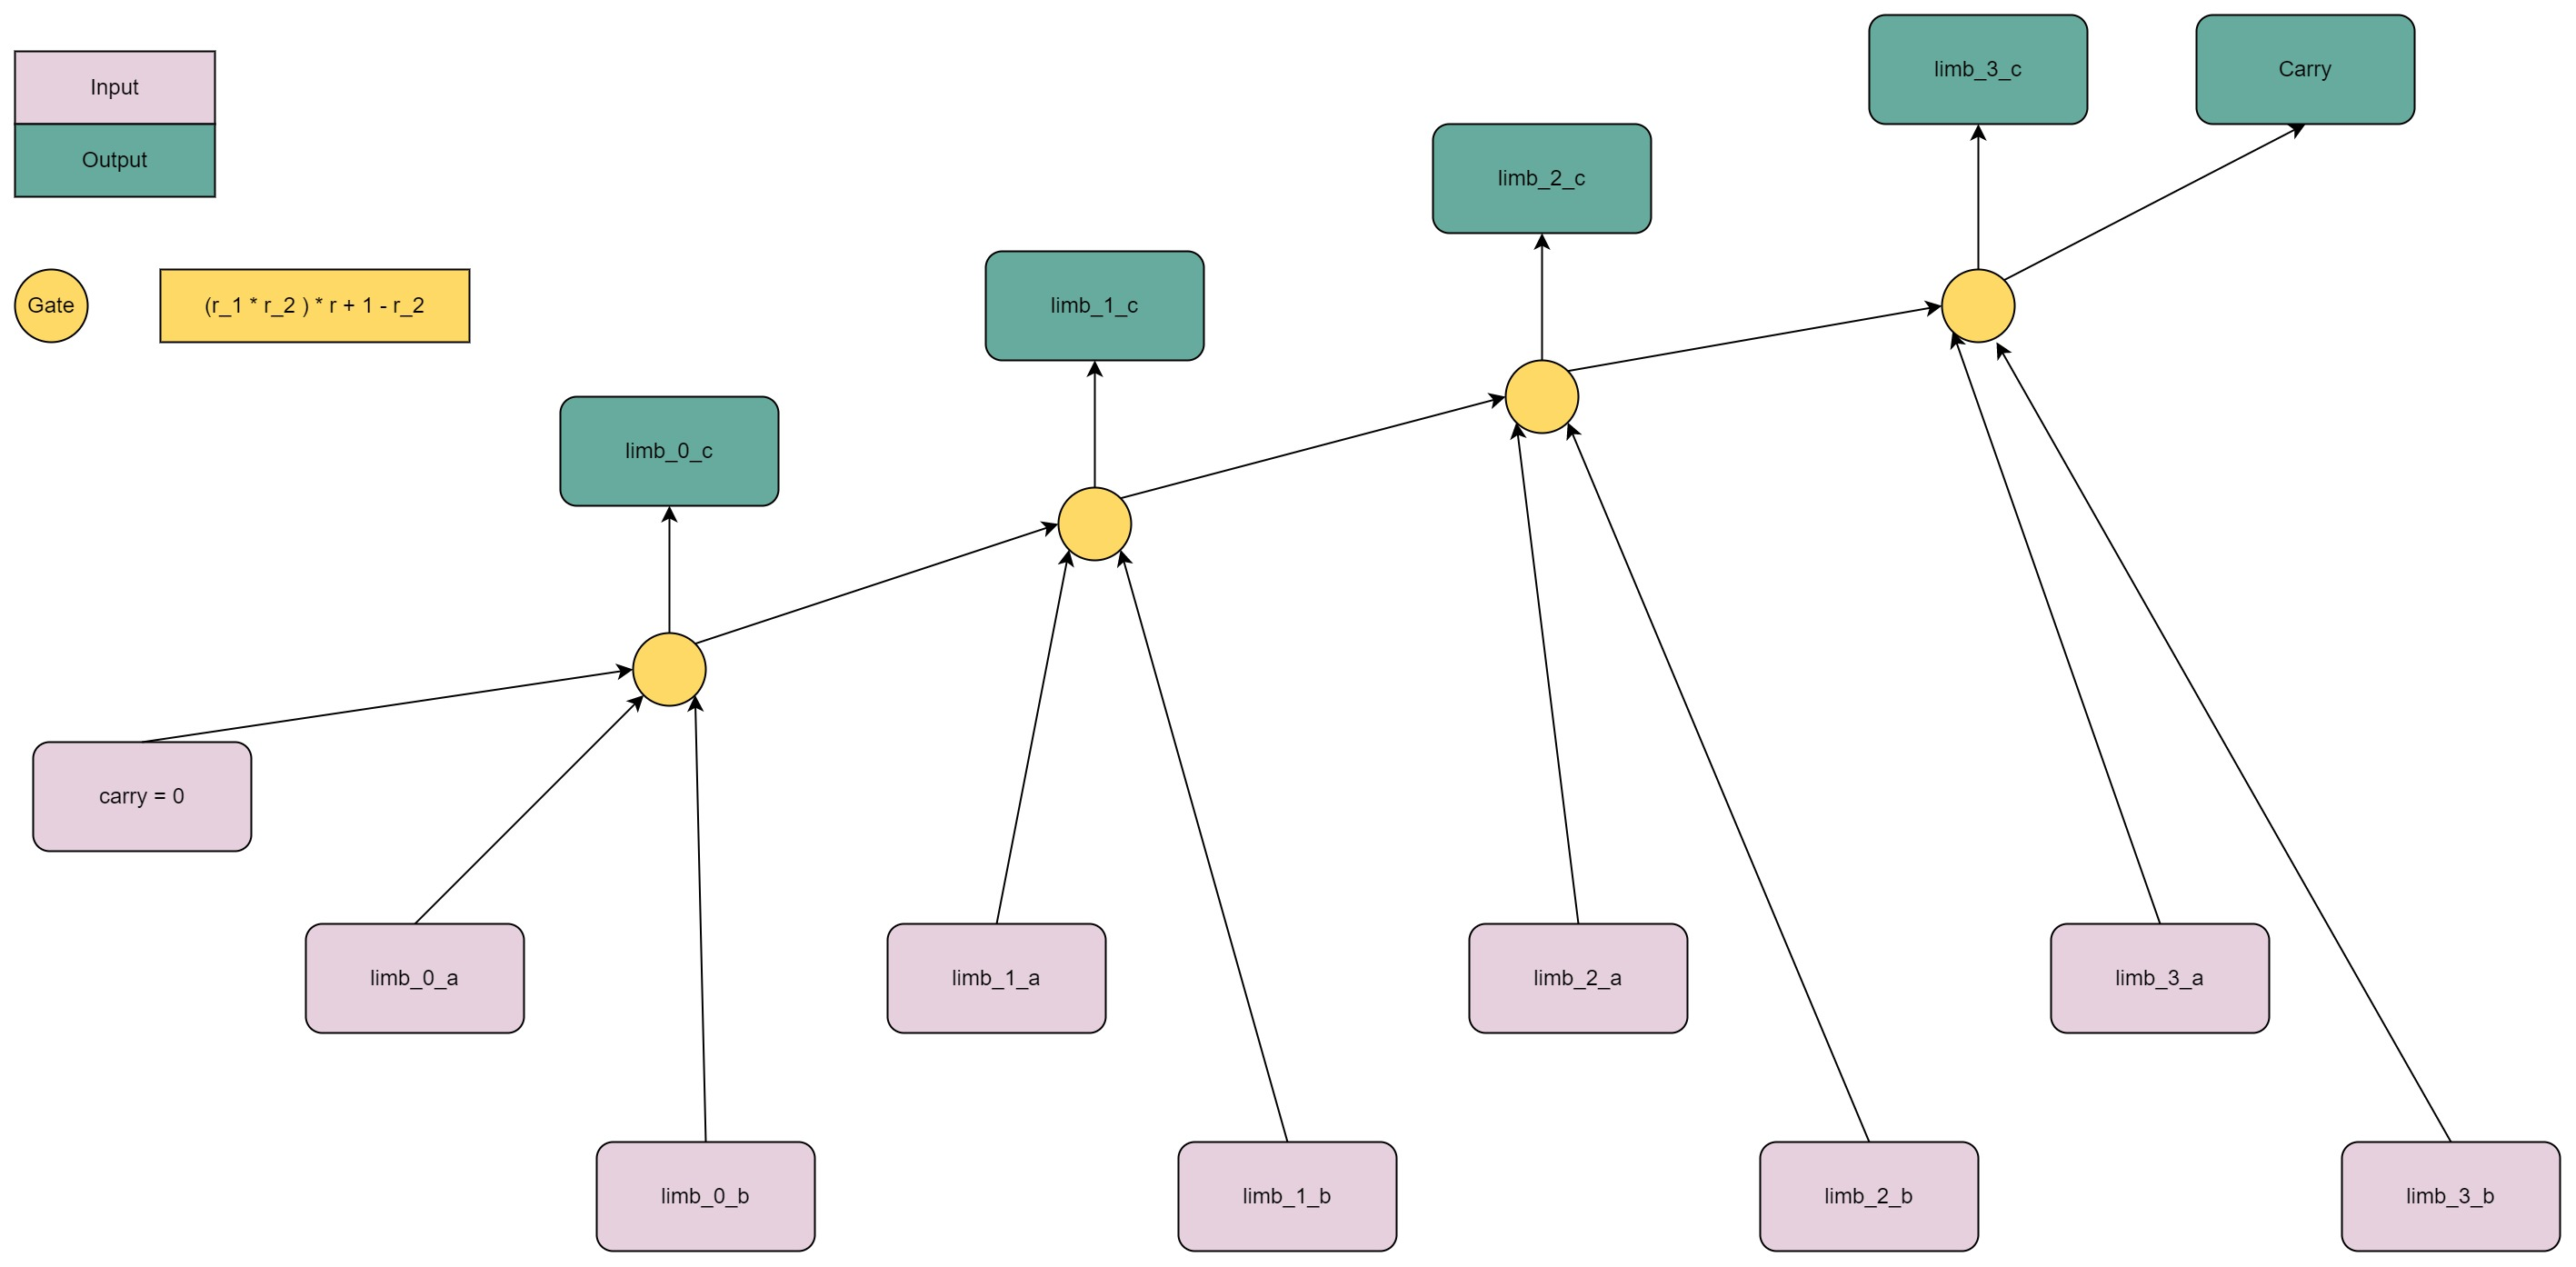
\includegraphics[width=0.8\textwidth]{biguint-add-circuit-layout.jpg}
    \caption{biguint-add circuit layout}
    \label{fig:biguint-add-circuit-layout}
\end{figure}

\Par{Trace layout}
See \figref{fig:biguint-add-trace-layout}.
\begin{figure}[!ht]
    \centering
    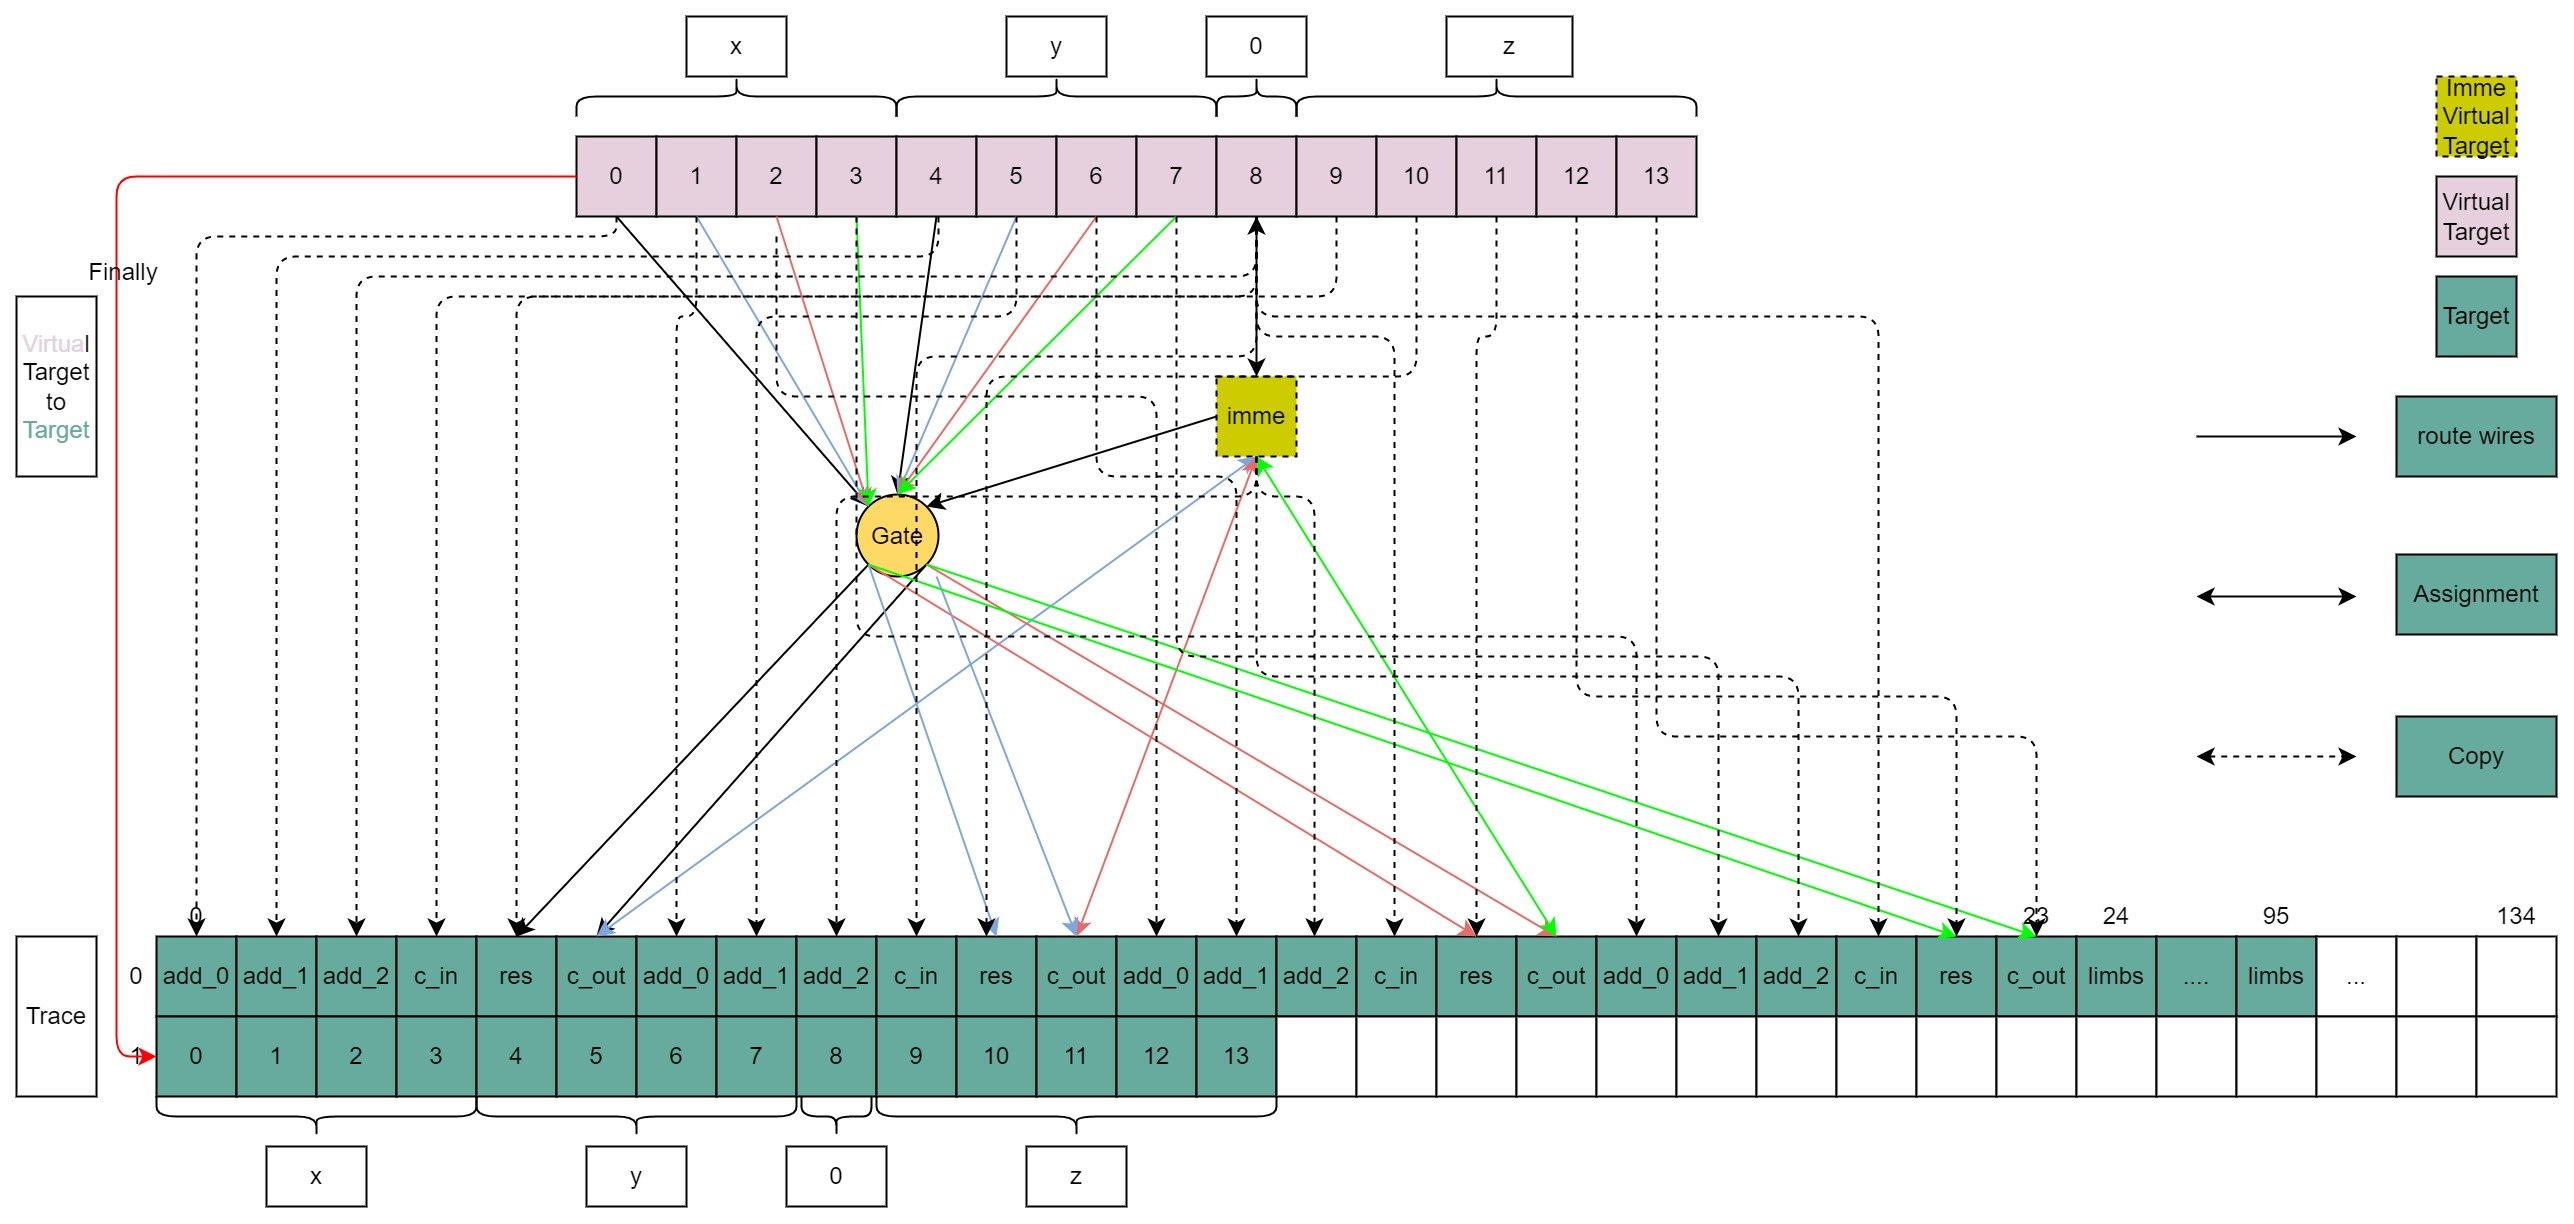
\includegraphics[width=0.8\textwidth]{biguint-add-trace-layout.jpg}
    \caption{biguint-add trace layout}
    \label{fig:biguint-add-trace-layout}
\end{figure}

\Par{Constraints info and costs}
\begin{itemize}
    \item gate type num: 1 (U32AddManyGate)
    \item gate ops num: limbs-num
    \item gate instance num: ceil(limbs-num / gate.ops)
    \item copy-constraints: limbs-num * 4
    \item max-degree: 4 (\verb|1 << limb-bits|)
\end{itemize}

\Par{Questions}
\begin{itemize}
    \item Why not make rangecheck constraint for inputs?
    \item Why not make copy constraint between cur-c-in and last-c-out?
\end{itemize}

    \subsubsection{biguint-sub}

\Par{Target}
Implement the substraction of two biguints.

\Par{Constraints logic}
\begin{itemize}
    \item Equation for gate;
    \item Sumcheck for ouptput;
    \item Rangecheck for limbs.
\end{itemize}

\Par{Circuit layout}
See \figref{fig:biguint-sub-circuit-layout}.
\begin{figure}[!ht]
    \centering
    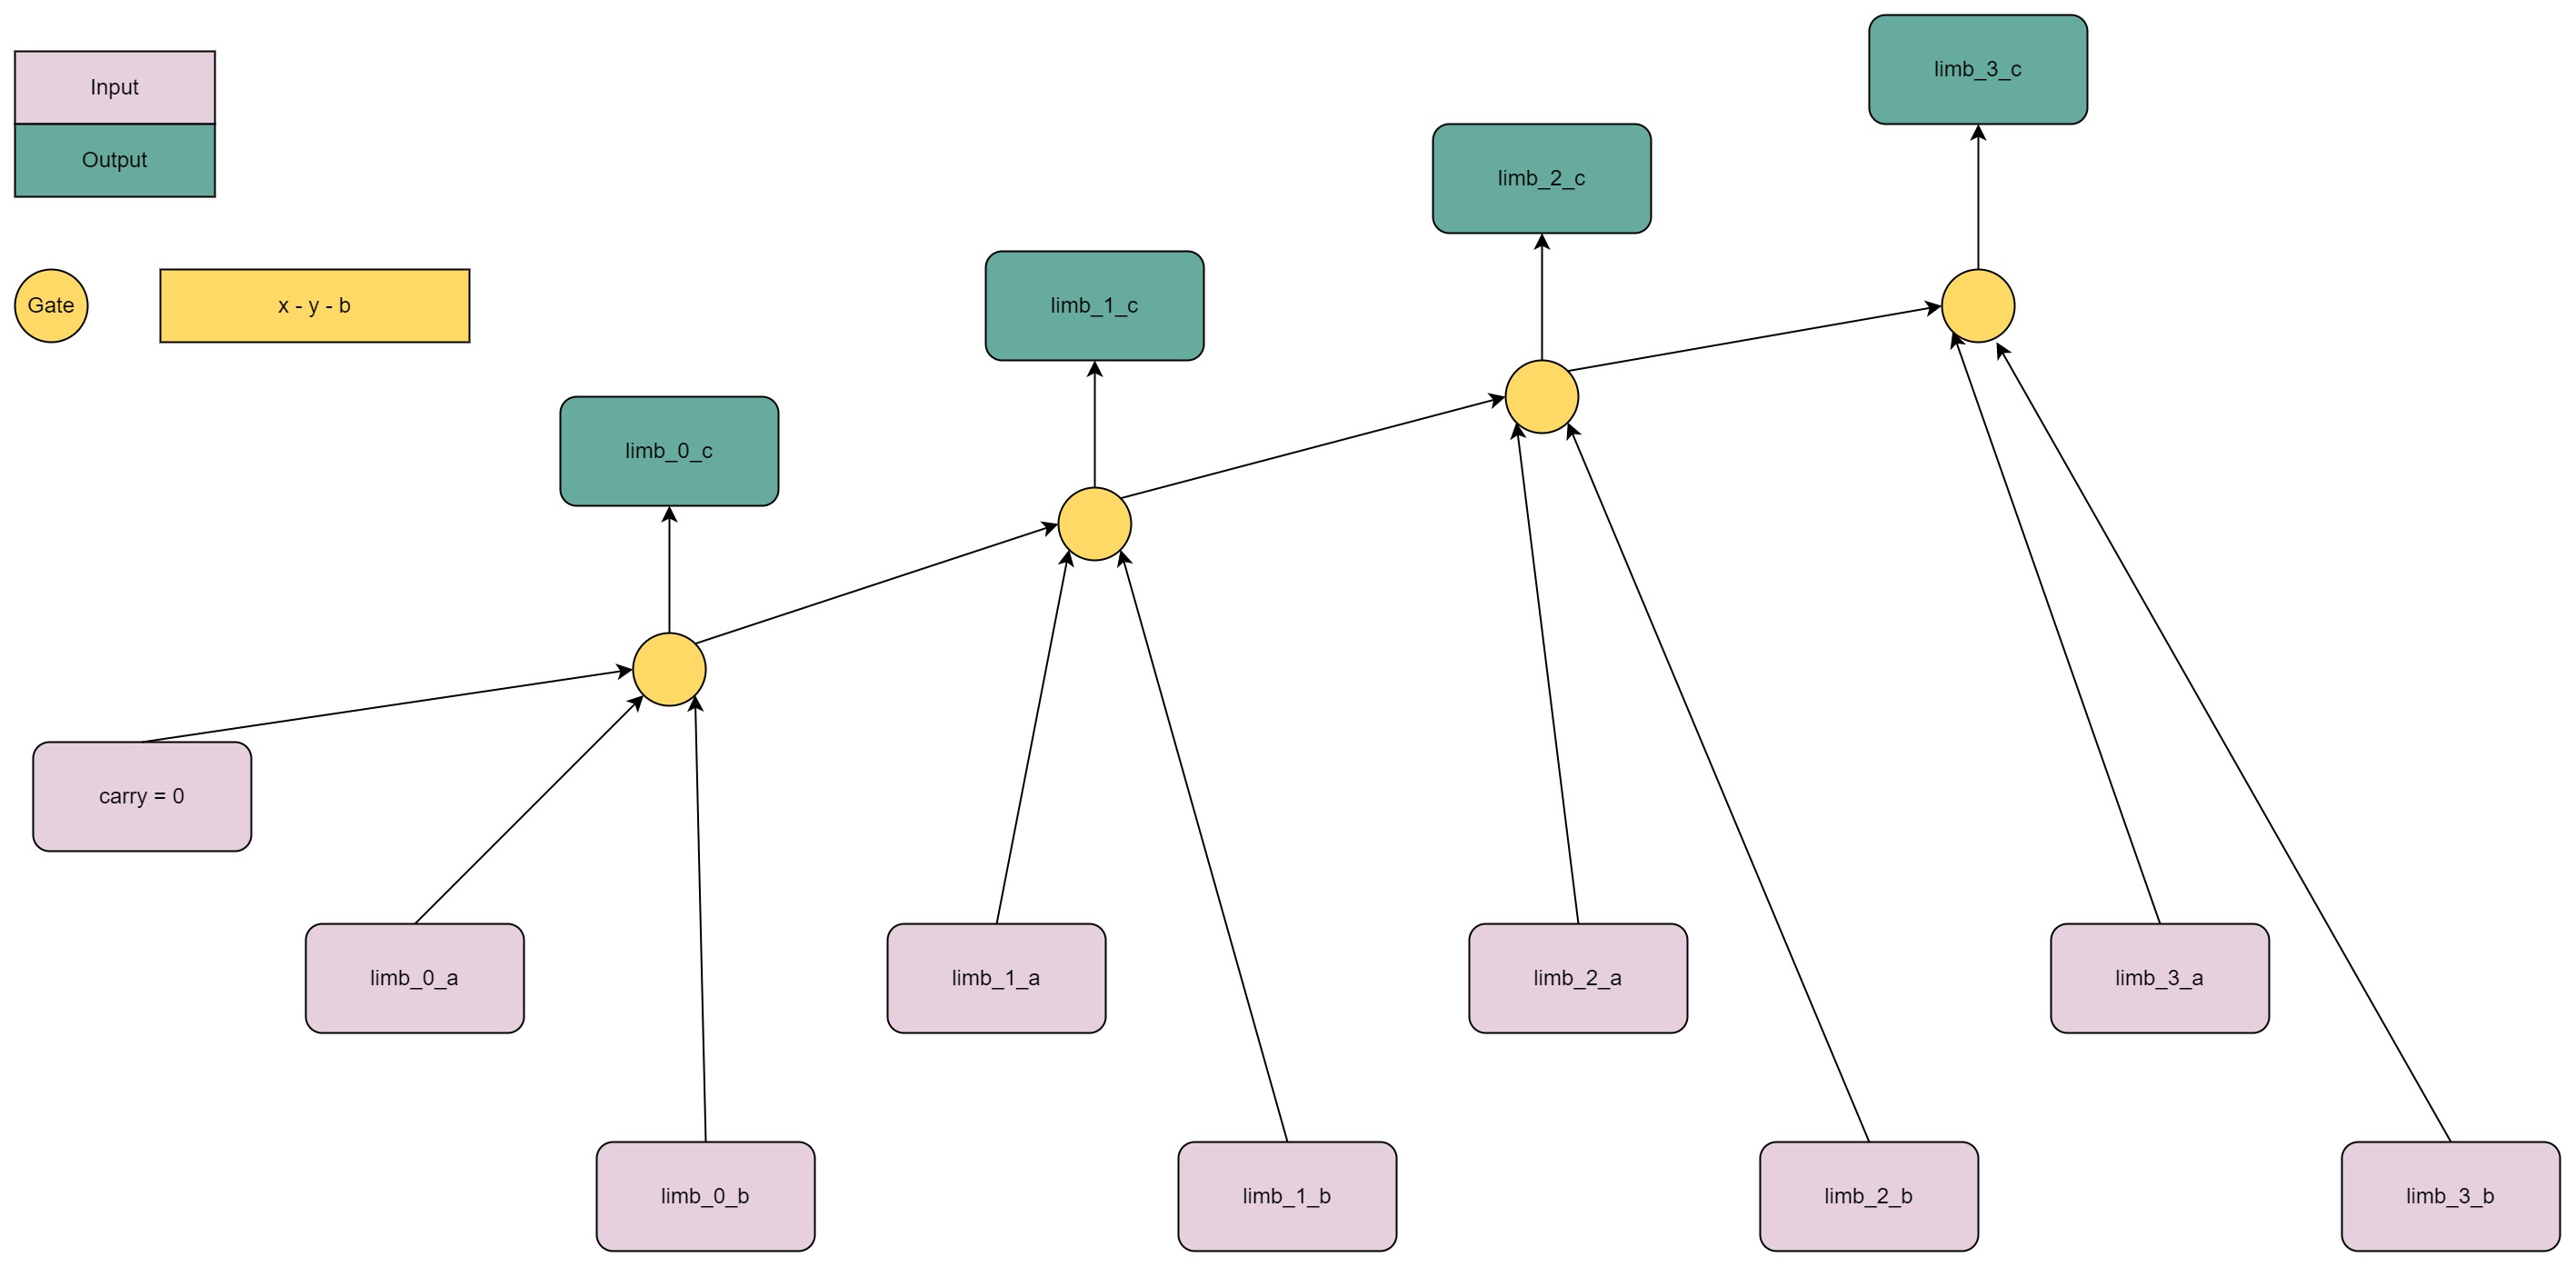
\includegraphics[width=0.8\textwidth]{biguint-sub-circuit-layout.jpg}
    \caption{biguint-sub circuit layout}
    \label{fig:biguint-sub-circuit-layout}
\end{figure}

\Par{Trace layout}
See \figref{fig:biguint-sub-trace-layout}.
\begin{figure}[!ht]
    \centering
    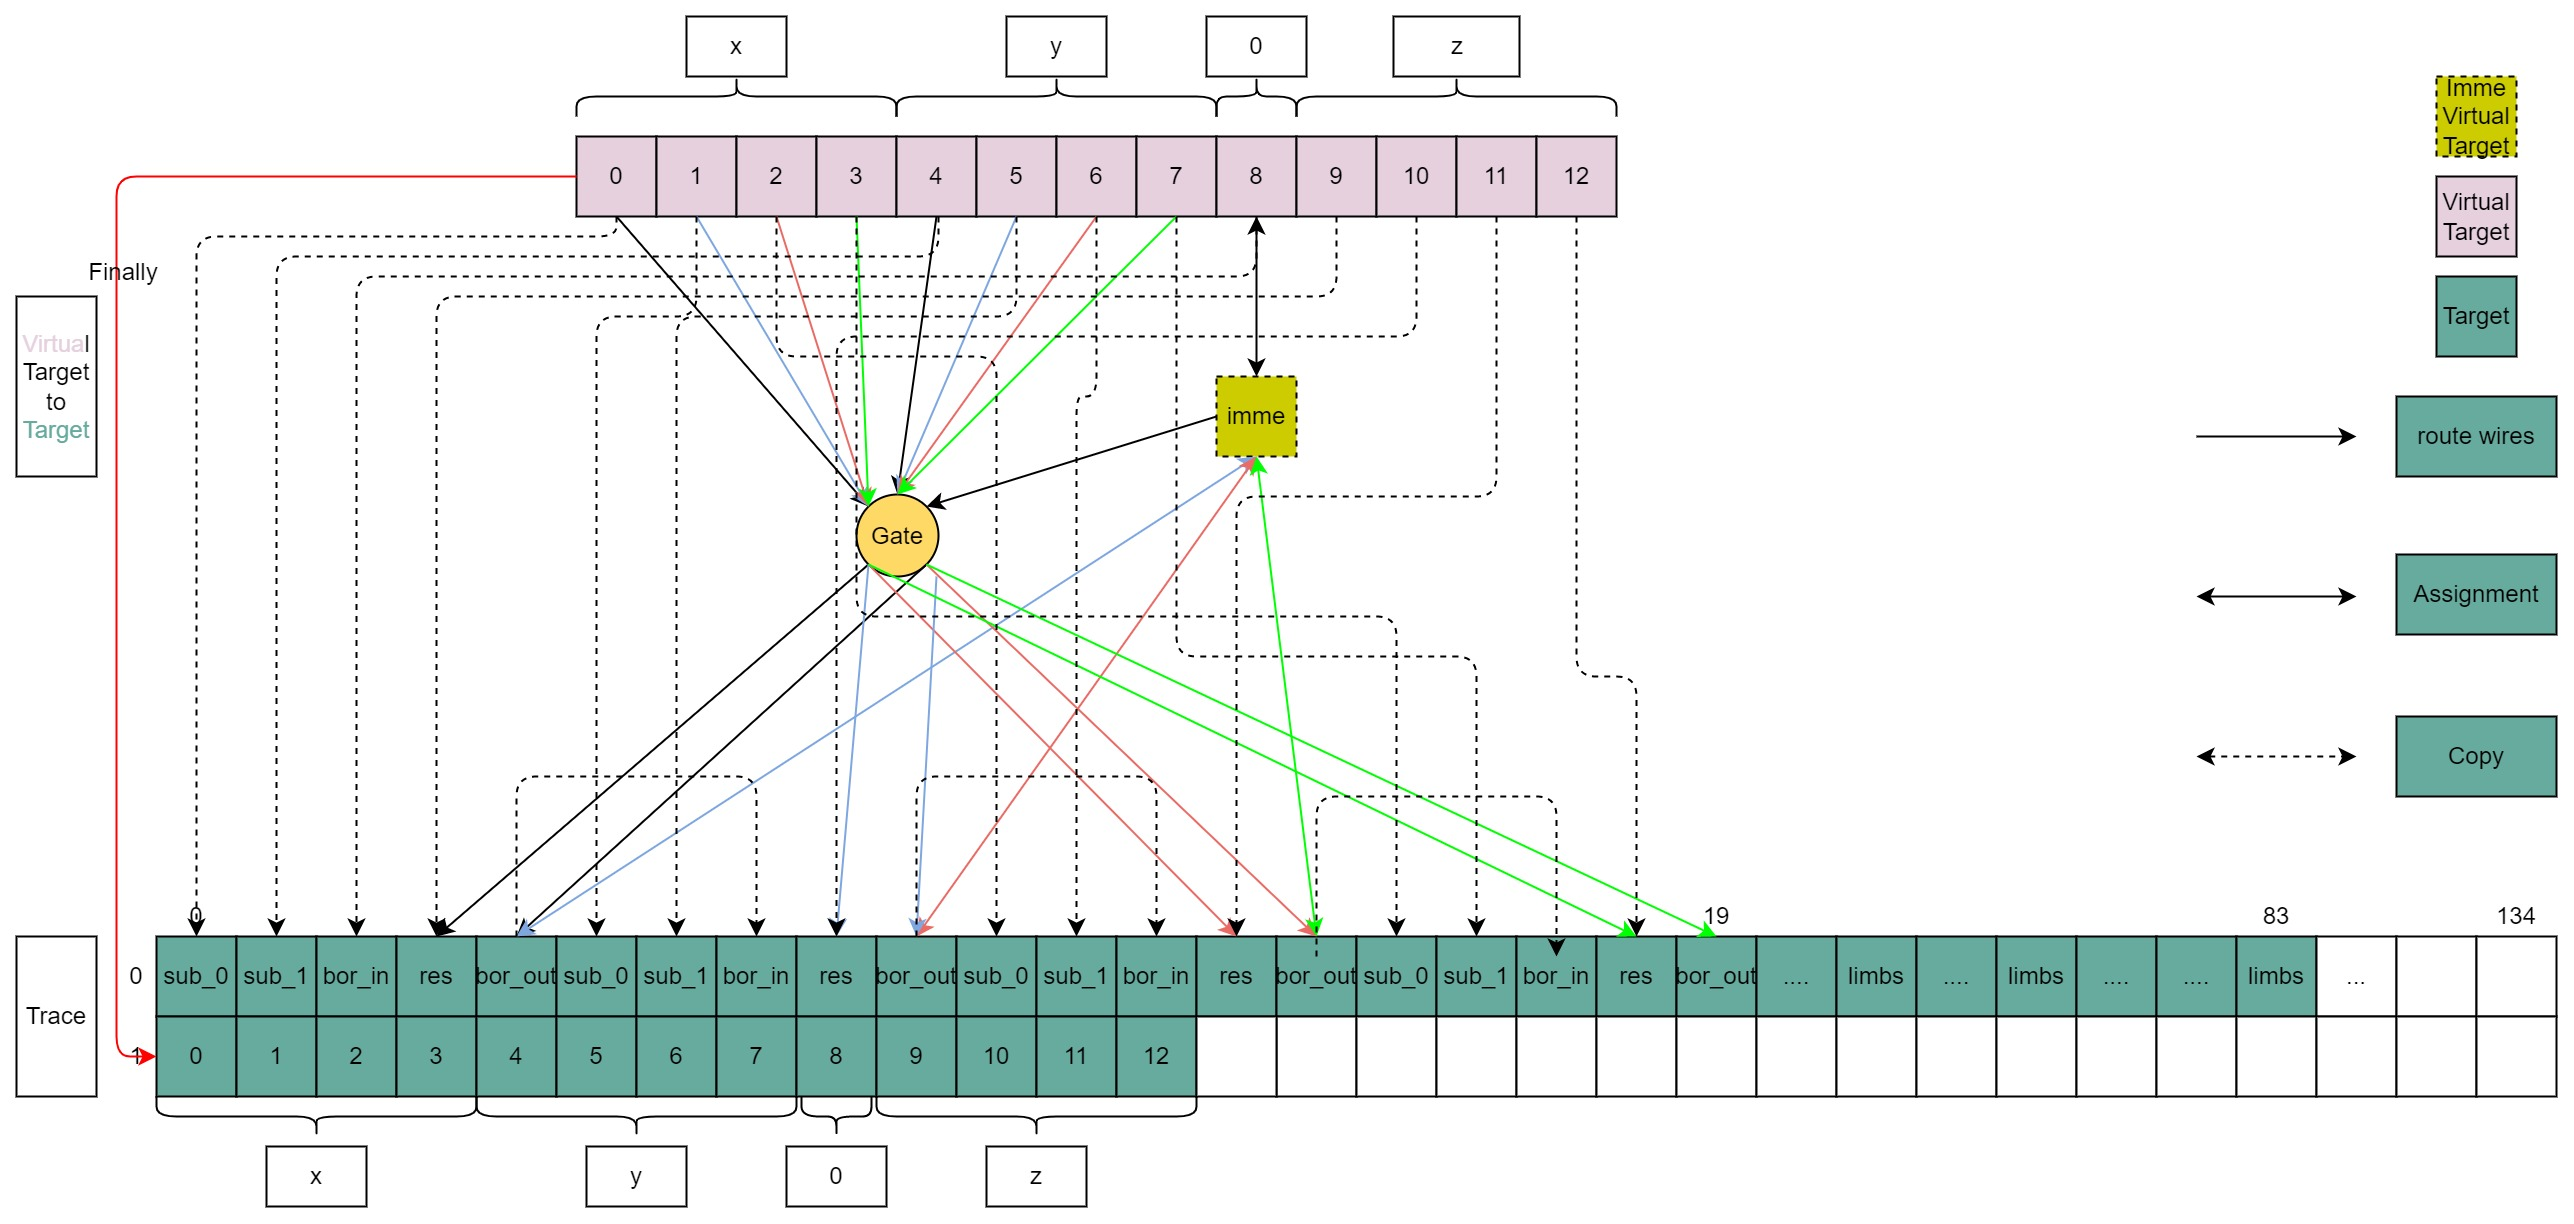
\includegraphics[width=0.8\textwidth]{biguint-sub-trace-layout.jpg}
    \caption{biguint-sub trace layout}
    \label{fig:biguint-sub-trace-layout}
\end{figure}

\Par{Constraints info and costs}
\begin{itemize}
    \item constraints-num: $6 \times (3 + 32 / 2) = 114$
    \item copy-constraints: $16$
    \item max-degree: $4$
    \item wires-num: $6 \times (5 + 16) = 126$
\end{itemize}

\Par{Questions}
\begin{itemize}
    \item Why not make rangecheck constraint for inputs?
    \item Could try to use the same constraint with add-gate.
\end{itemize}

    \subsubsection{biguint-mul}

\Par{Target}
Implement the multiplication of two biguints.

\Par{Constraints logic}
\begin{itemize}
    \item Compute mul-factors first, use U32ArithmeticGate;
    \item Add mul-factors from low bits, use U32AddManyGate.
\end{itemize}

\Par{Process layout}
See \figref{fig:biguint-mul-layout}
\begin{figure}[!ht]
    \centering
    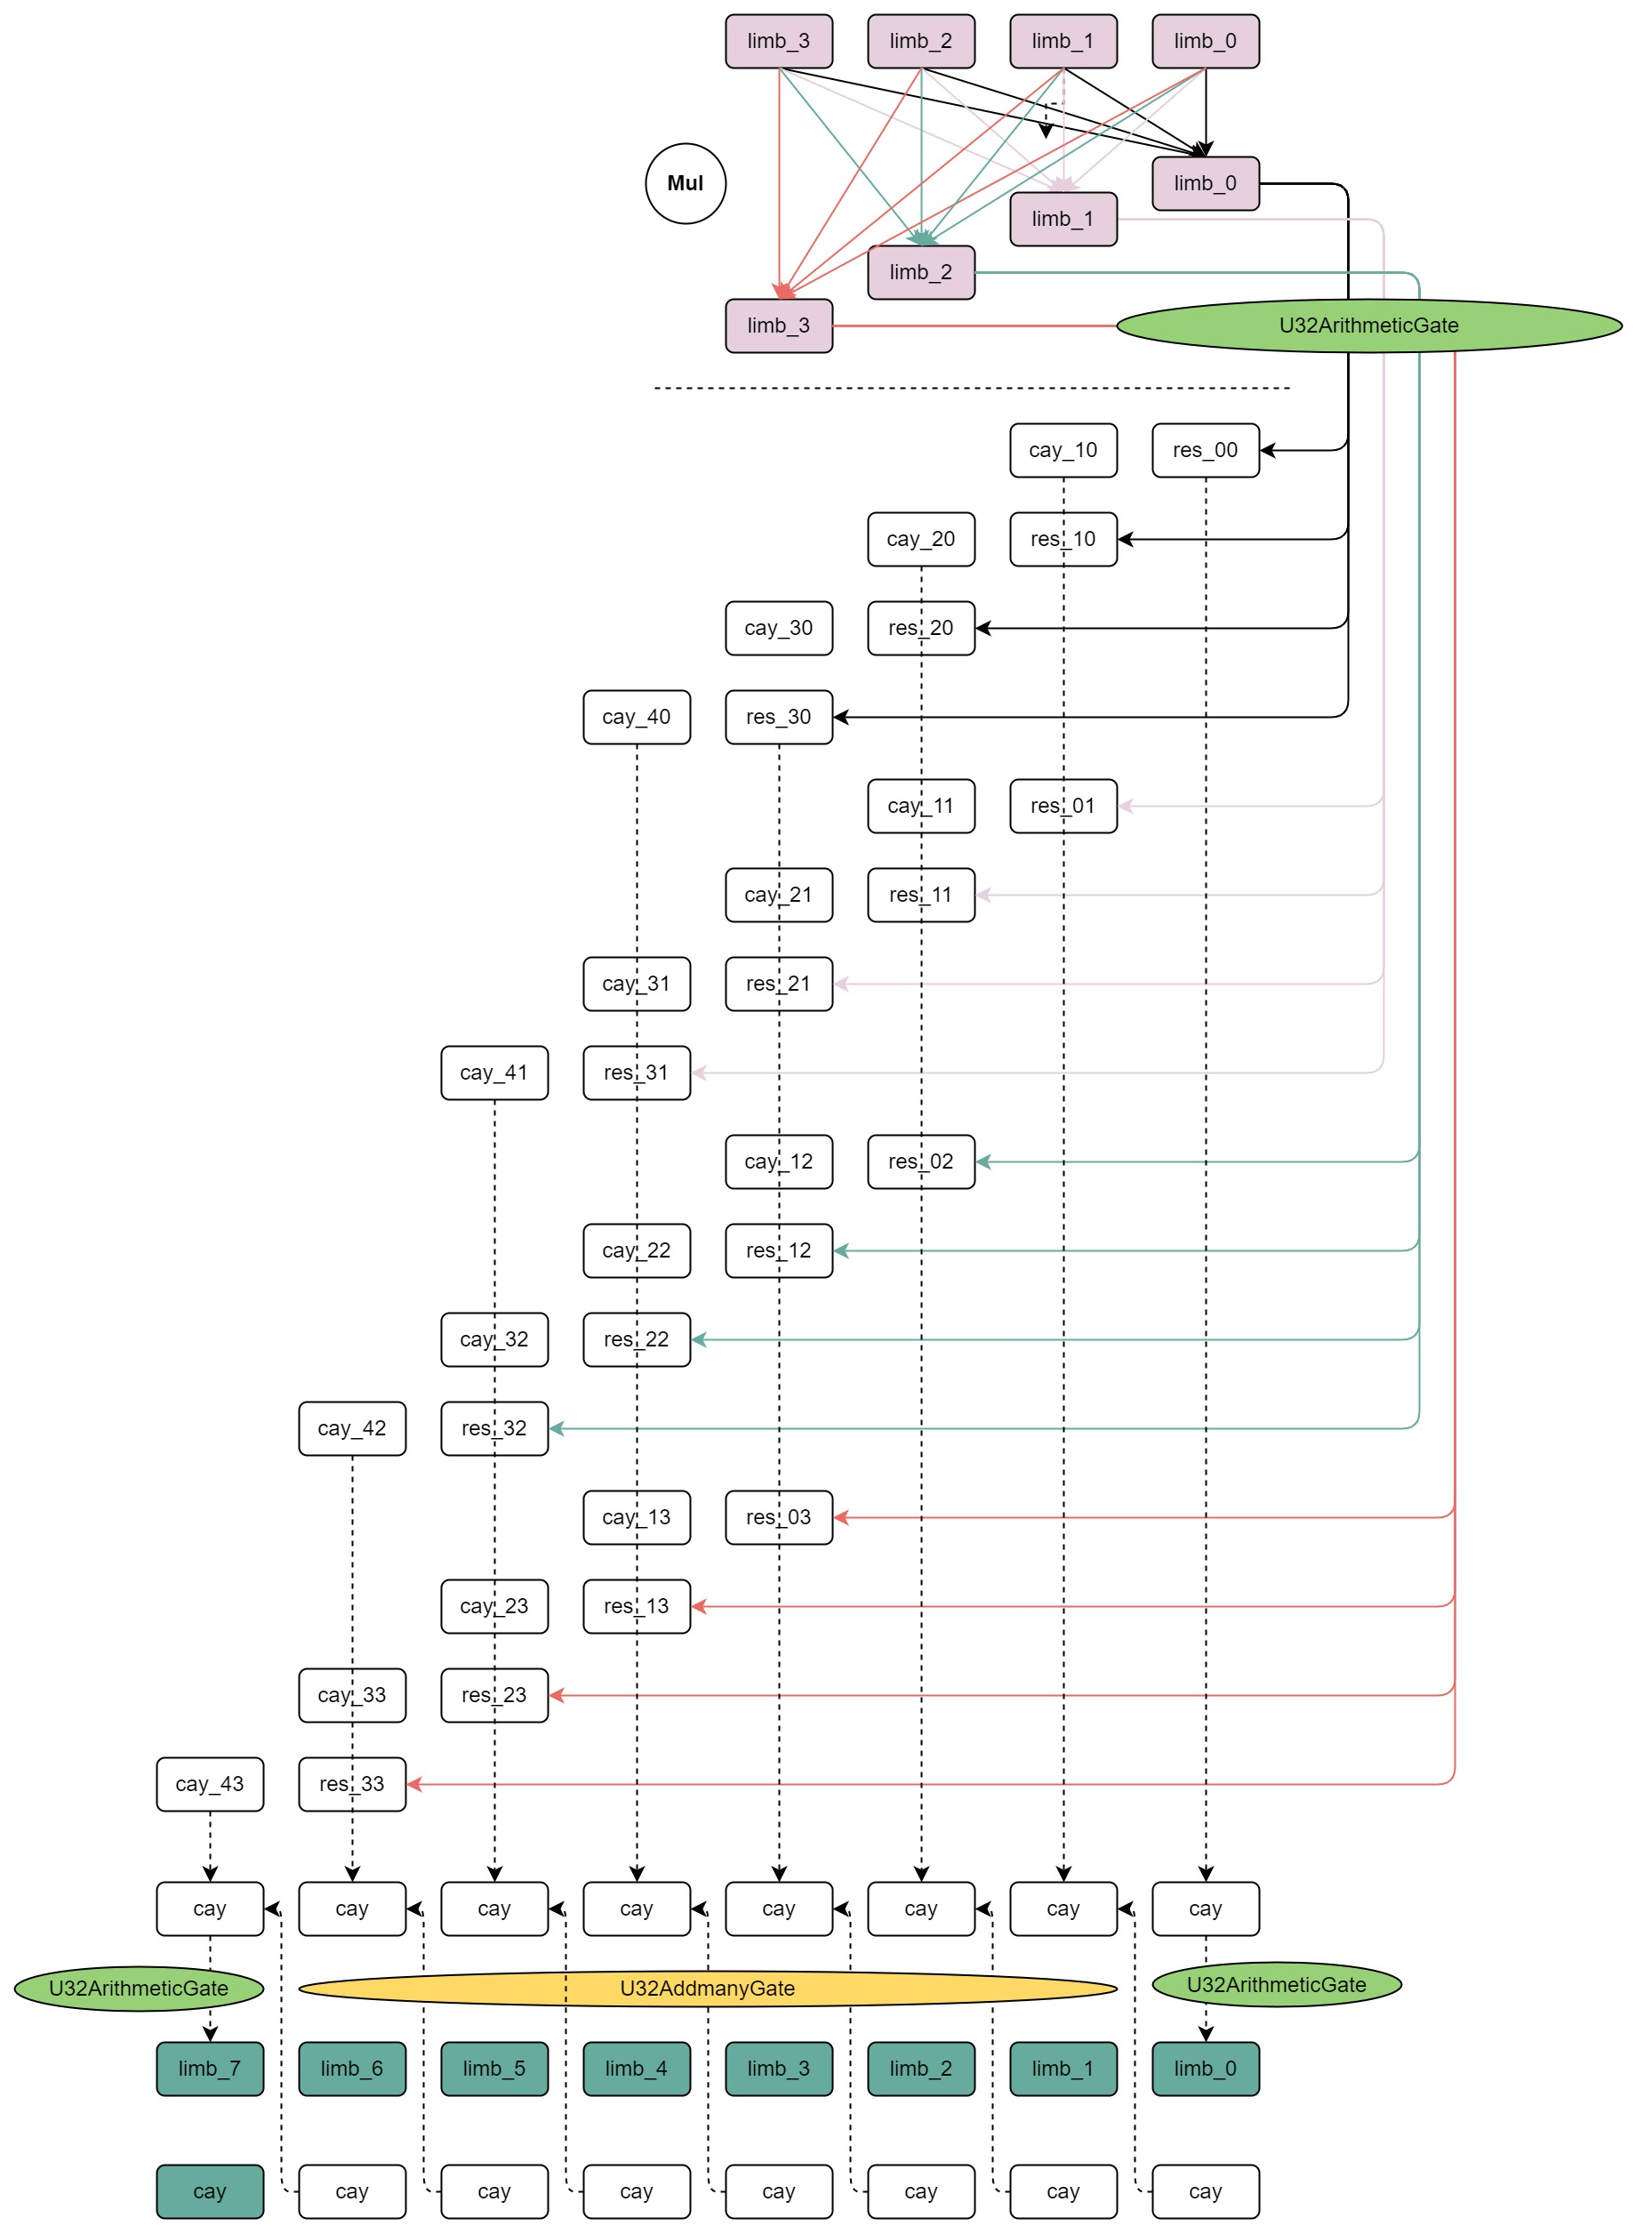
\includegraphics[width=0.8\textwidth]{biguint-mul-layout.jpg}
    \caption{biguint-mul layout}
    \label{fig:biguint-mul-layout}
\end{figure}

\Par{Constraints info and costs}
\begin{itemize}
    \item Gate type num: 4 (U32ArithmeticGate, U32AddManyGate(num-addends: 4), U32AddManyGate(num-addends: 6), U32AddManyGate(num-addends: 8))
    \item Gate instance num: 9
    \item U32ArithmeticGate num: 6
    \item U32AddManyGate num: 3
    \item copy-constraints: $18 \times 3 + (4 + 6 + 8) \times 2 + 9 = 99$
    \item max-degree: 4
\end{itemize}

    \section{biguint-div}
\label{biguint-div}

Note that div-rem has the same constraints logic with div

\begin{enumerate}
    \item target
        \begin{itemize}
            \item implement the division of two biguints
        \end{itemize}
    \item constraints-logic
        \begin{itemize}
            \item not implement div-algrithem directly
            \item use nondeterministic feature to check div-logic
            \item check div * b + rem = a
            \item check rem < b
        \end{itemize}
    \item div-process layout
        \begin{figure}[!ht]
            \centering
            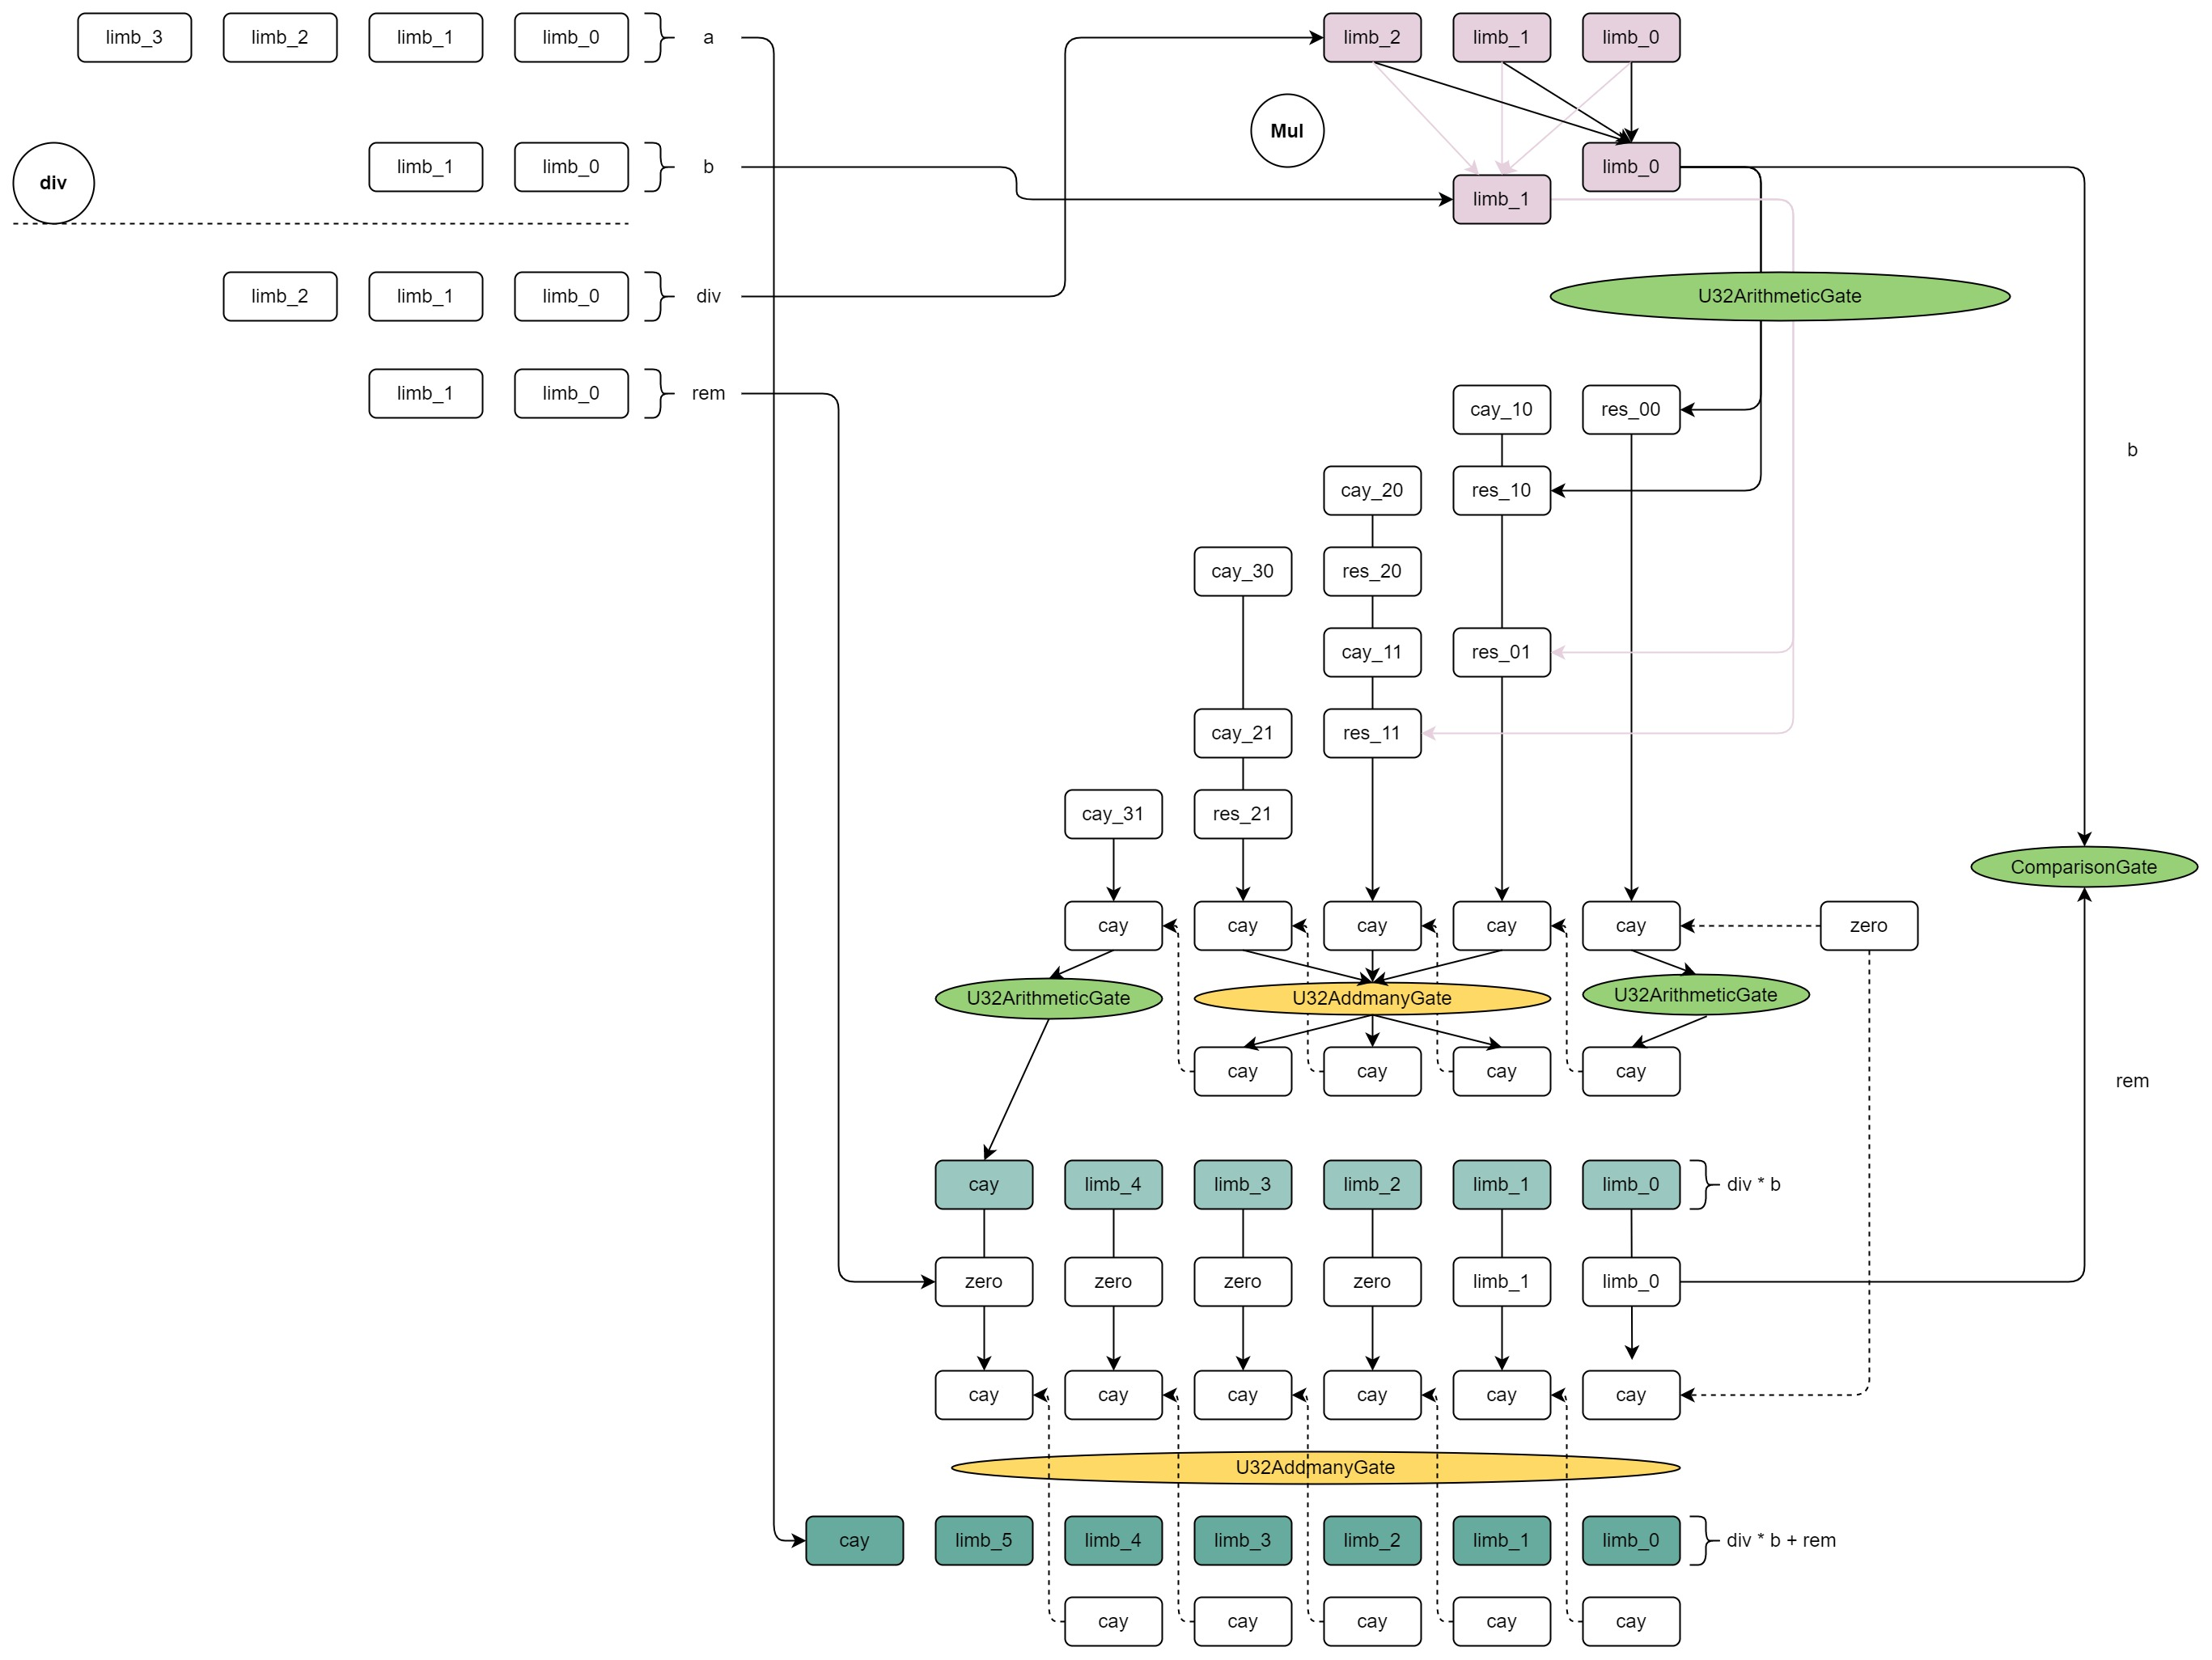
\includegraphics[width=0.8\textwidth]{biguint-div-layout.jpg}
            \caption{biguint-div layout.jpg}
            \label{fig:biguint-div-layout.jpg}
        \end{figure}
    
    \item constraints-info and costs
        \begin{itemize}
            \item Gate type num: 5(U32ArithmeticGate, U32AddManyGate(num-addends: 3), U32AddManyGate(num-addends: 4), ComparisionGate, ArithmeticGate)
            \item Gate instance num: 3 + 3 + 4 + 3 = 13 
            \item U32ArithmeticGate num: 3
            \item U32AddManyGate num: 3
            \item ComparisionGate num: 4
            \item ArithmeticGate num: 3
            \item copy-constraints: 3 * 8 + 4 + 5 + 4 + 4 * 6 + 7 + 1 + 26 + 5 = 100 
            \item max-degree: 4
        \end{itemize}

\end{enumerate}
    \subsubsection{biguint-cmp}

\Par{Target}
Implement the comparison of two biguints.

\Par{Constraints logic}
\begin{itemize}
    \item Split the input to many limbs, such that: \verb|limbs_num = bits / chunks|;
    \item Execute comparison for low bits limbs;
    \item Ensure that the result is determined by the highest limbs which are not equal.
\end{itemize}

\Par{Process layout}
See \figref{fig:biguint-cmp-layout}.
\begin{figure}[!ht]
    \centering
    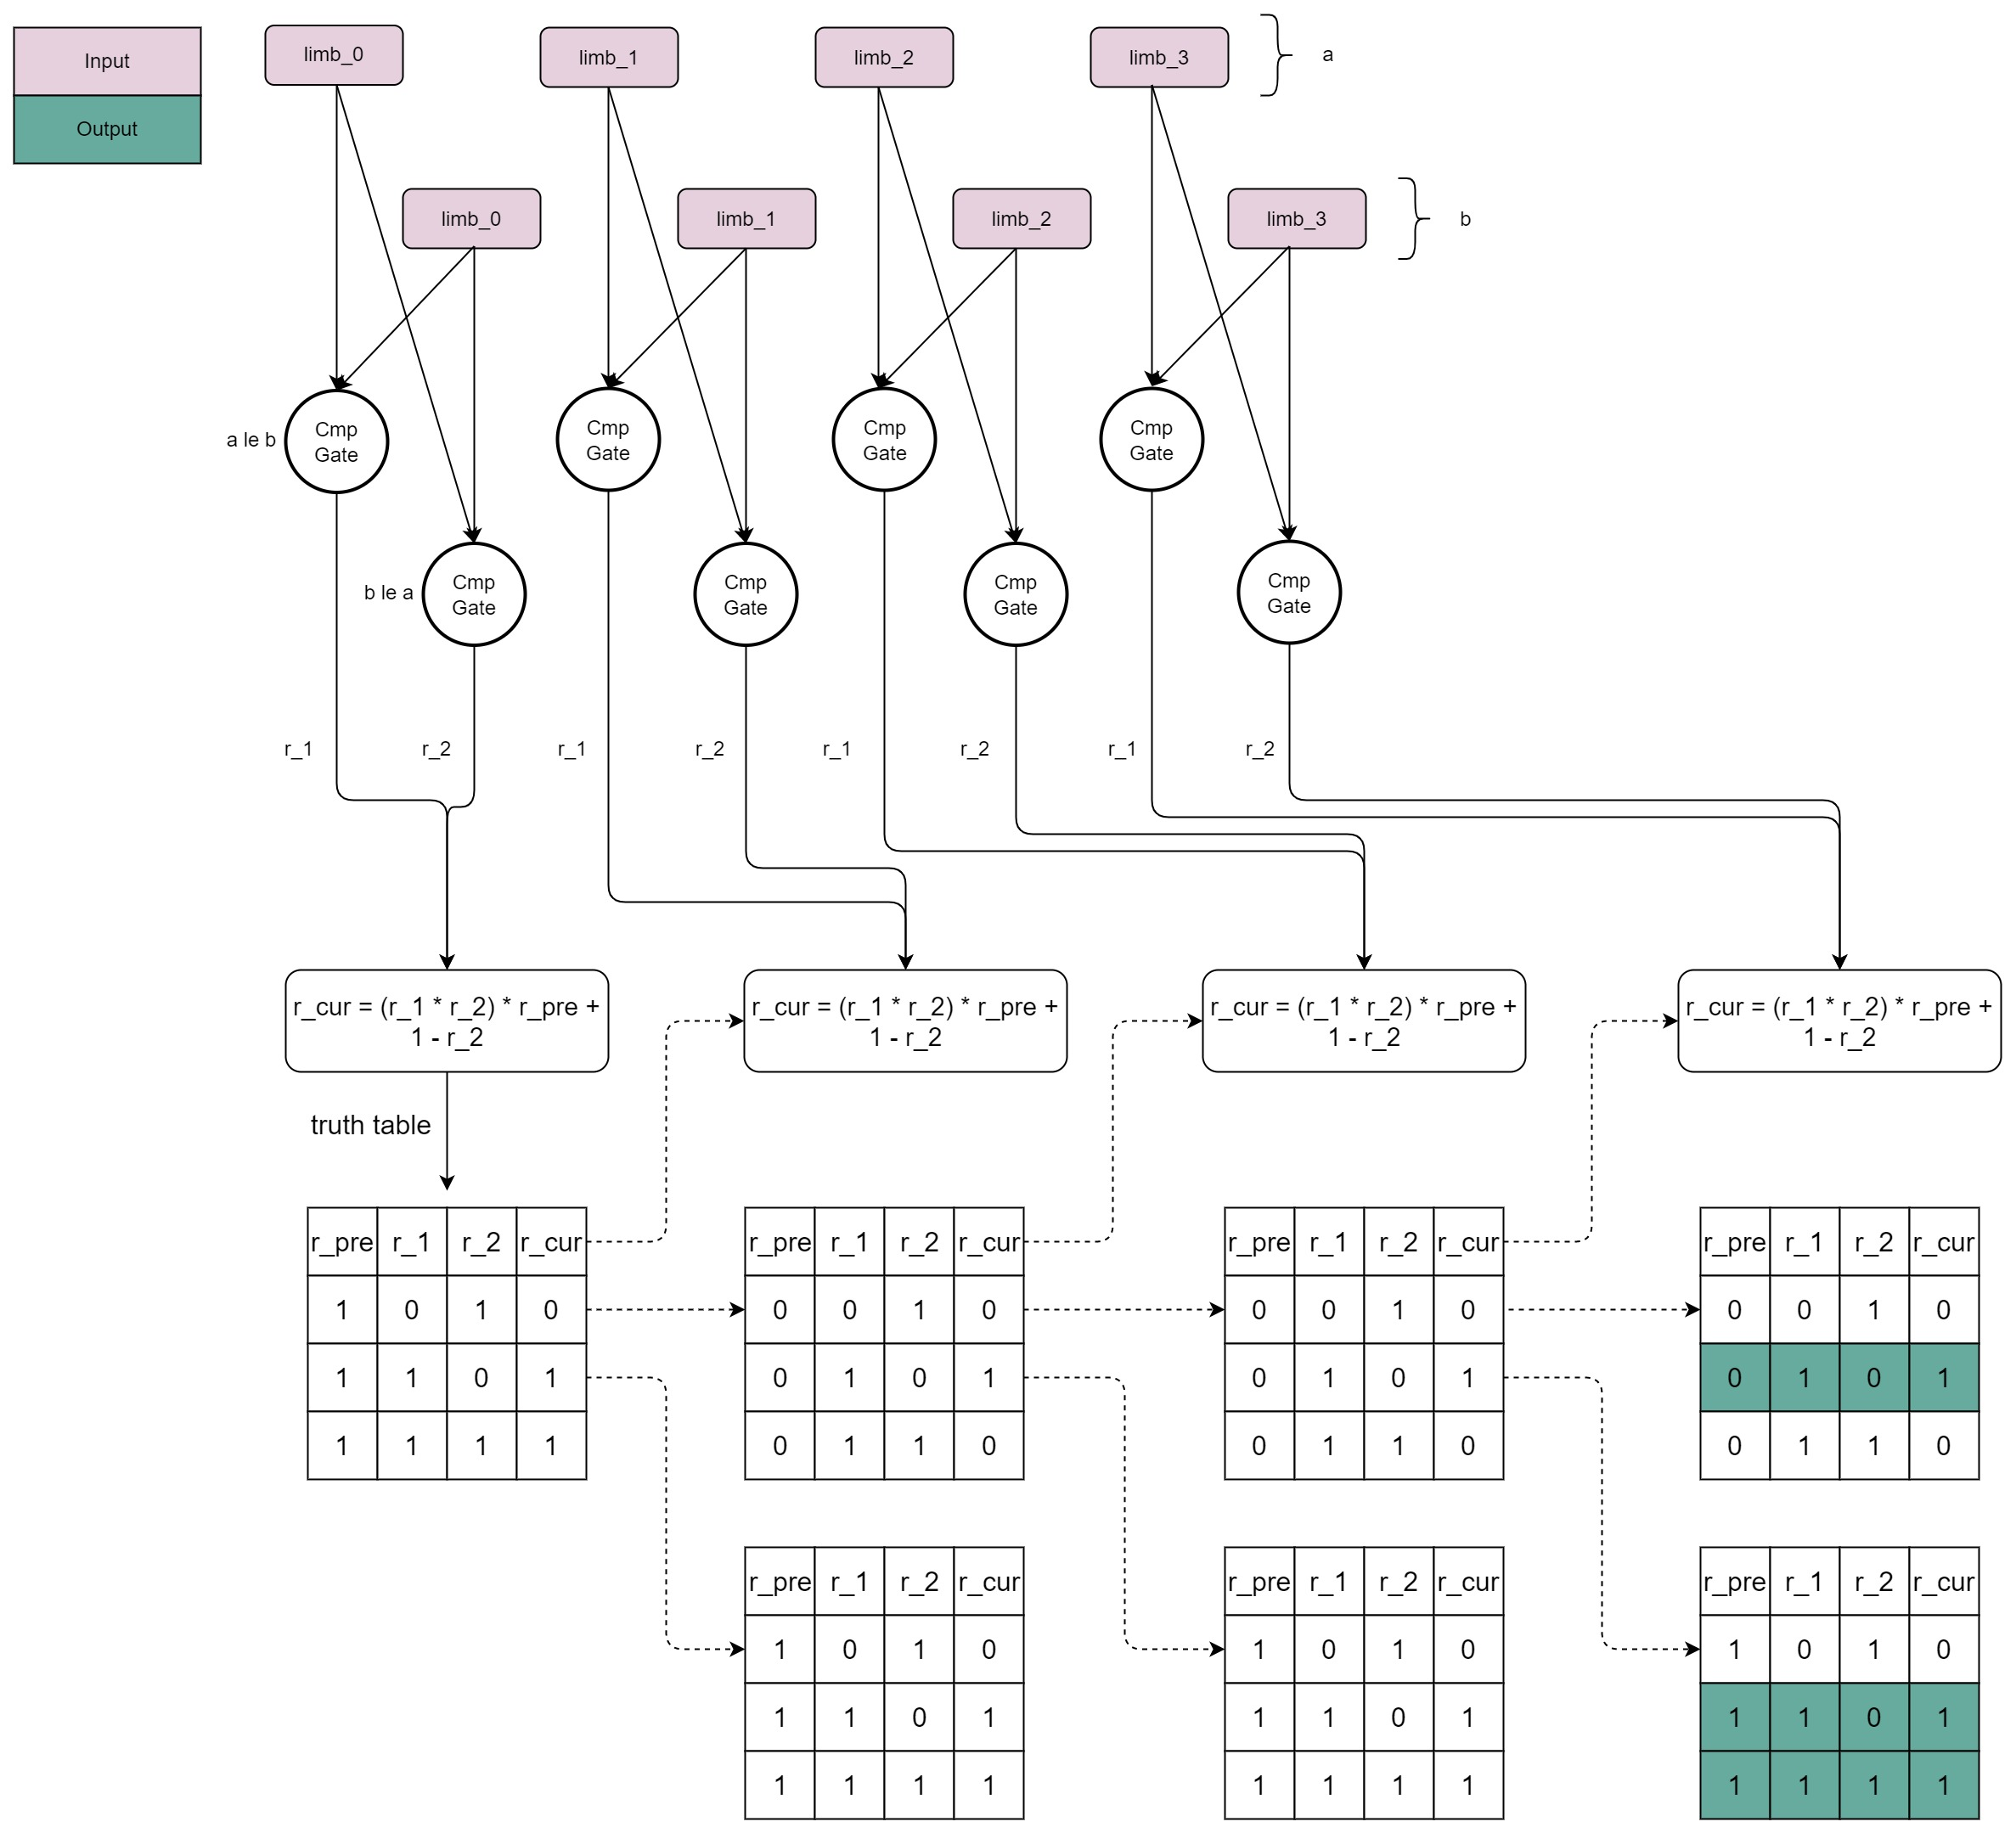
\includegraphics[width=0.8\textwidth]{biguint-cmp-layout.jpg}
    \caption{biguint-cmp layout}
    \label{fig:biguint-cmp-layout}
\end{figure}

\Par{Circuit layout}
See \figref{fig:biguint-cmp-circuit-layout}.
\begin{figure}[!ht]
    \centering
    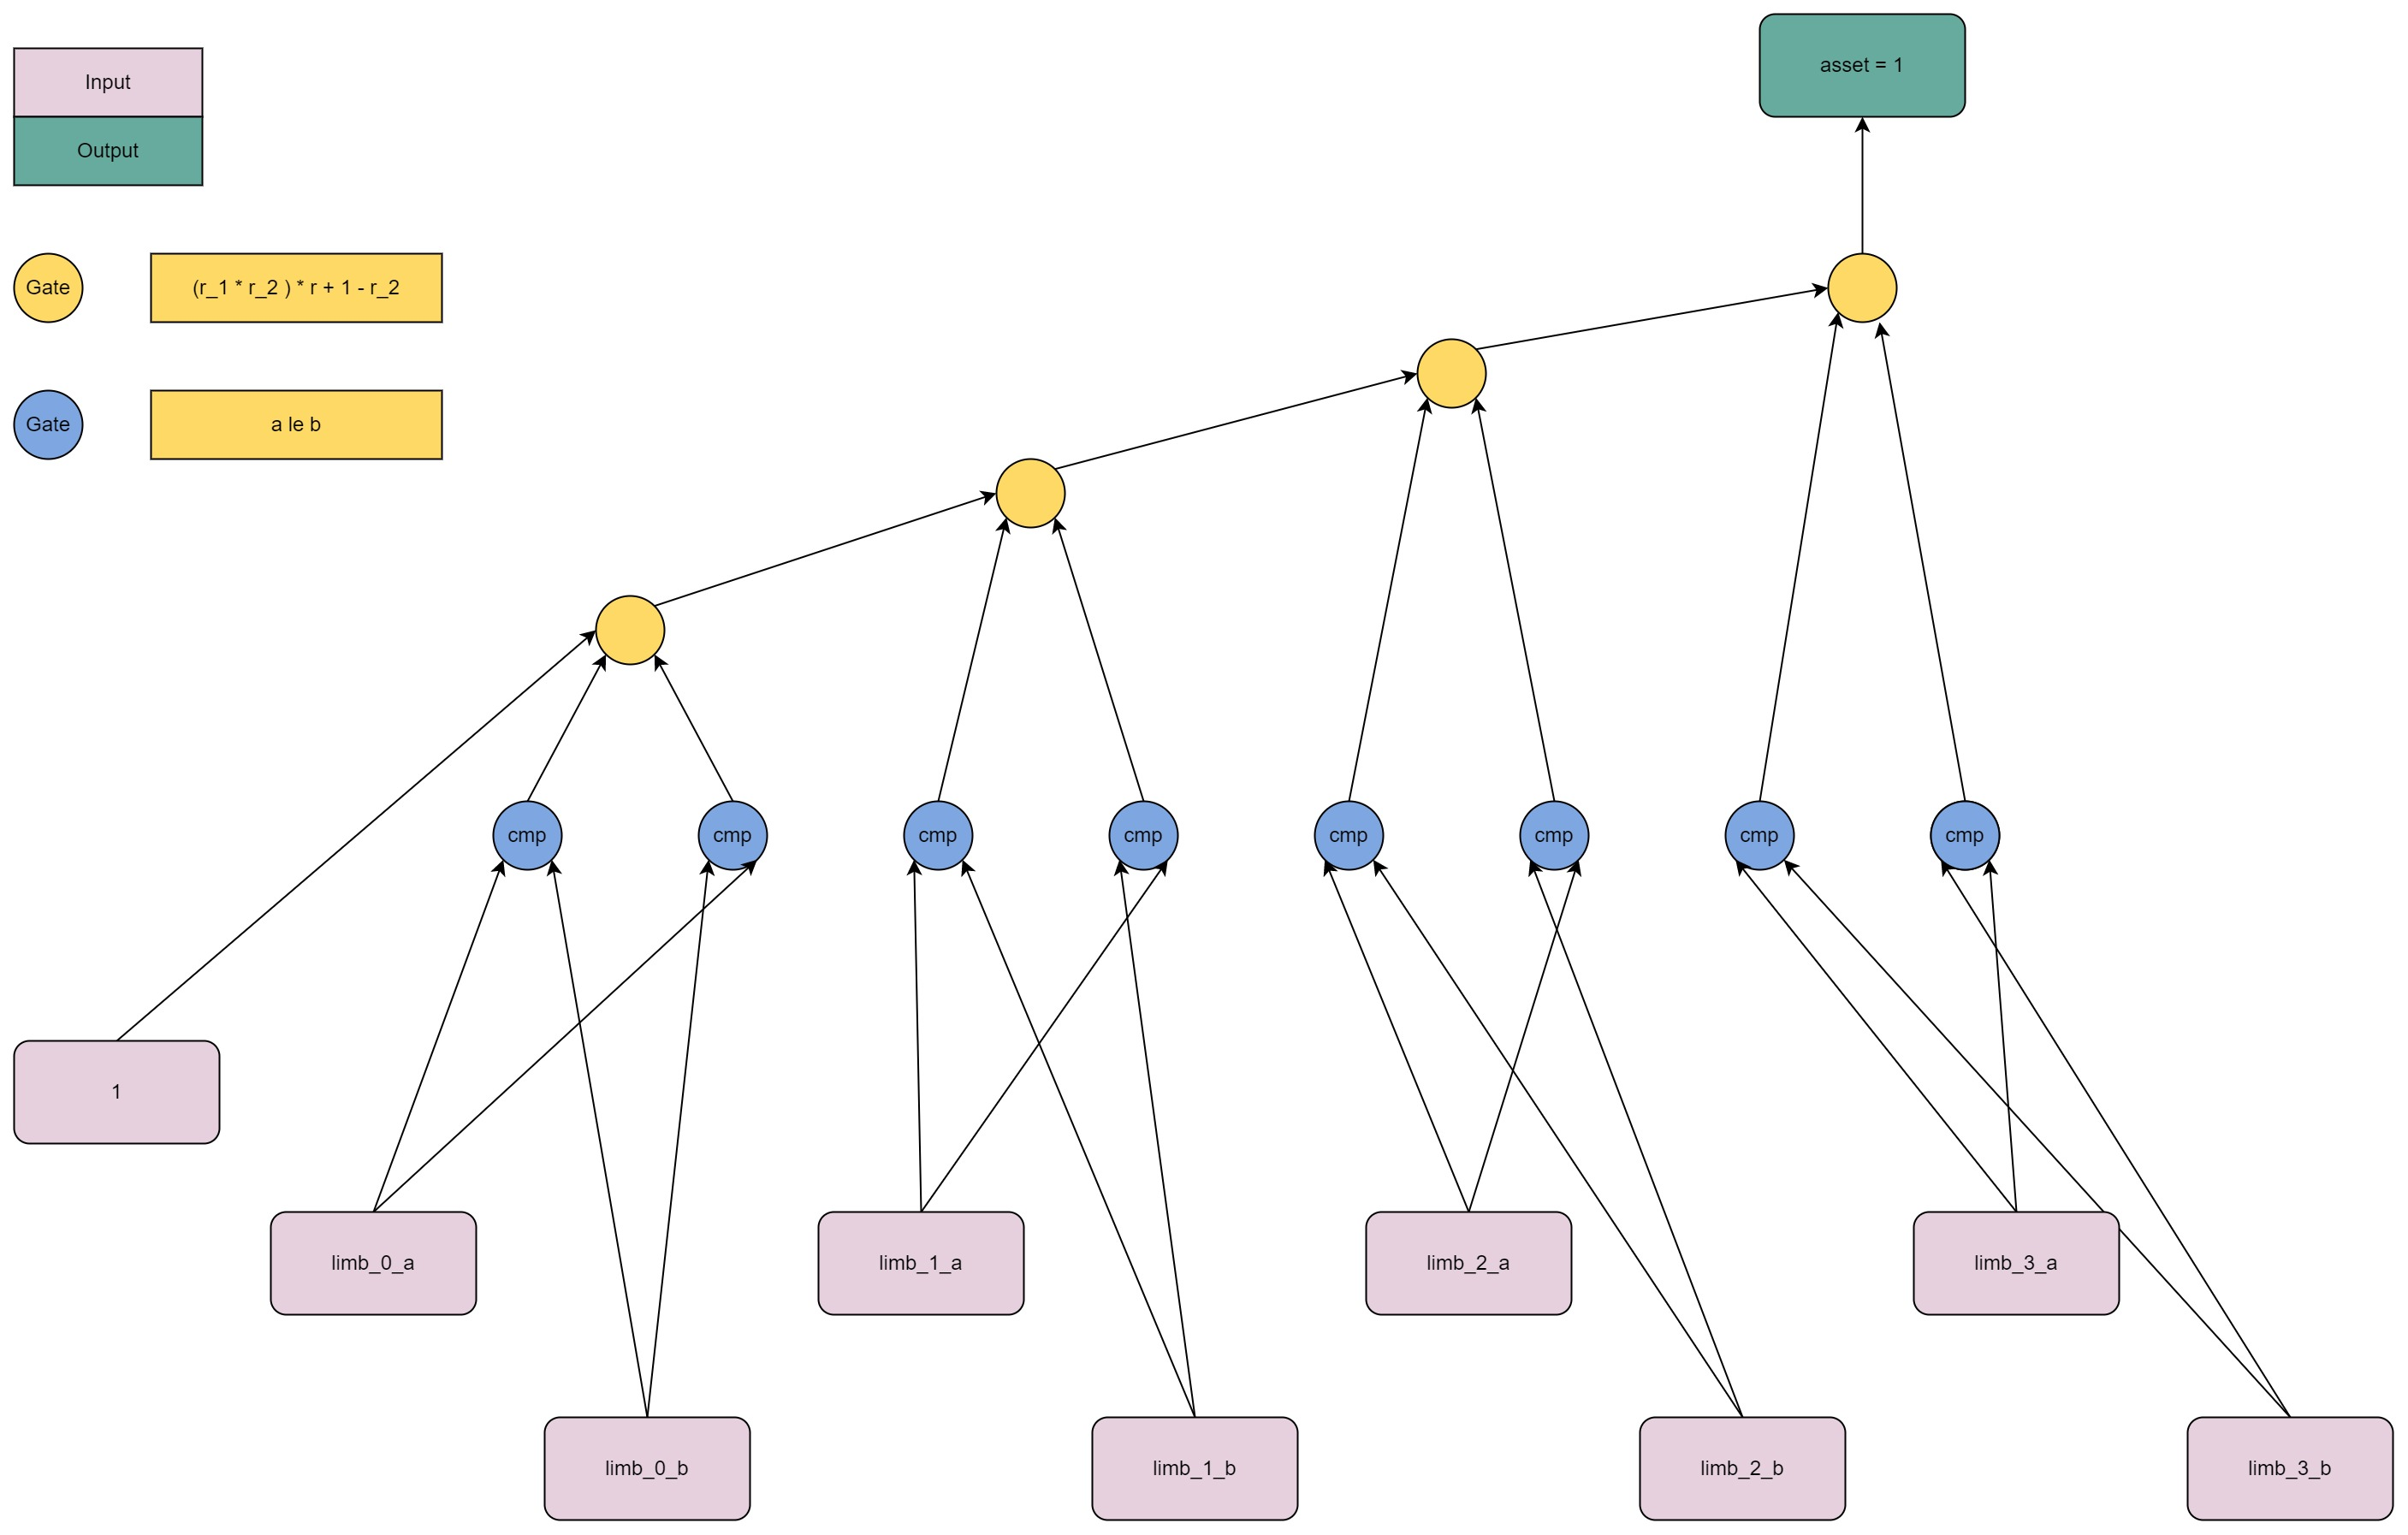
\includegraphics[width=0.8\textwidth]{biguint-cmp-circuit-layout.jpg}
    \caption{biguint-cmp circuit layout}
    \label{fig:biguint-cmp-circuit-layout}
\end{figure}

\Par{Constraints info and costs}
\begin{itemize}
    \item Gate type num: 2 (ComparisionGate, ArithmeticGate)
    \item Gate instance num: $4 \times 2 + 3 = 11$
    \item ComparisionGate num: 8
    \item ArithmeticGate num: 3
    \item copy-constraints: $(4 + 9) \times 4 + 1 = 53$
    \item max-degree: 4
\end{itemize}

    \subsubsection{nonnative-add}
\label{nonnative-add}

\begin{enumerate}
    \item target
        check the additional relation among three nonnative target objects.
    \item constraints-logic
        \begin{itemize}
            \item check equation for gadget,  a + b = c + modular * overflow
            \item check that "c lt modular"
        \end{itemize}
    \item nonnative-add process layout
        \begin{figure}[!ht]
            \centering
            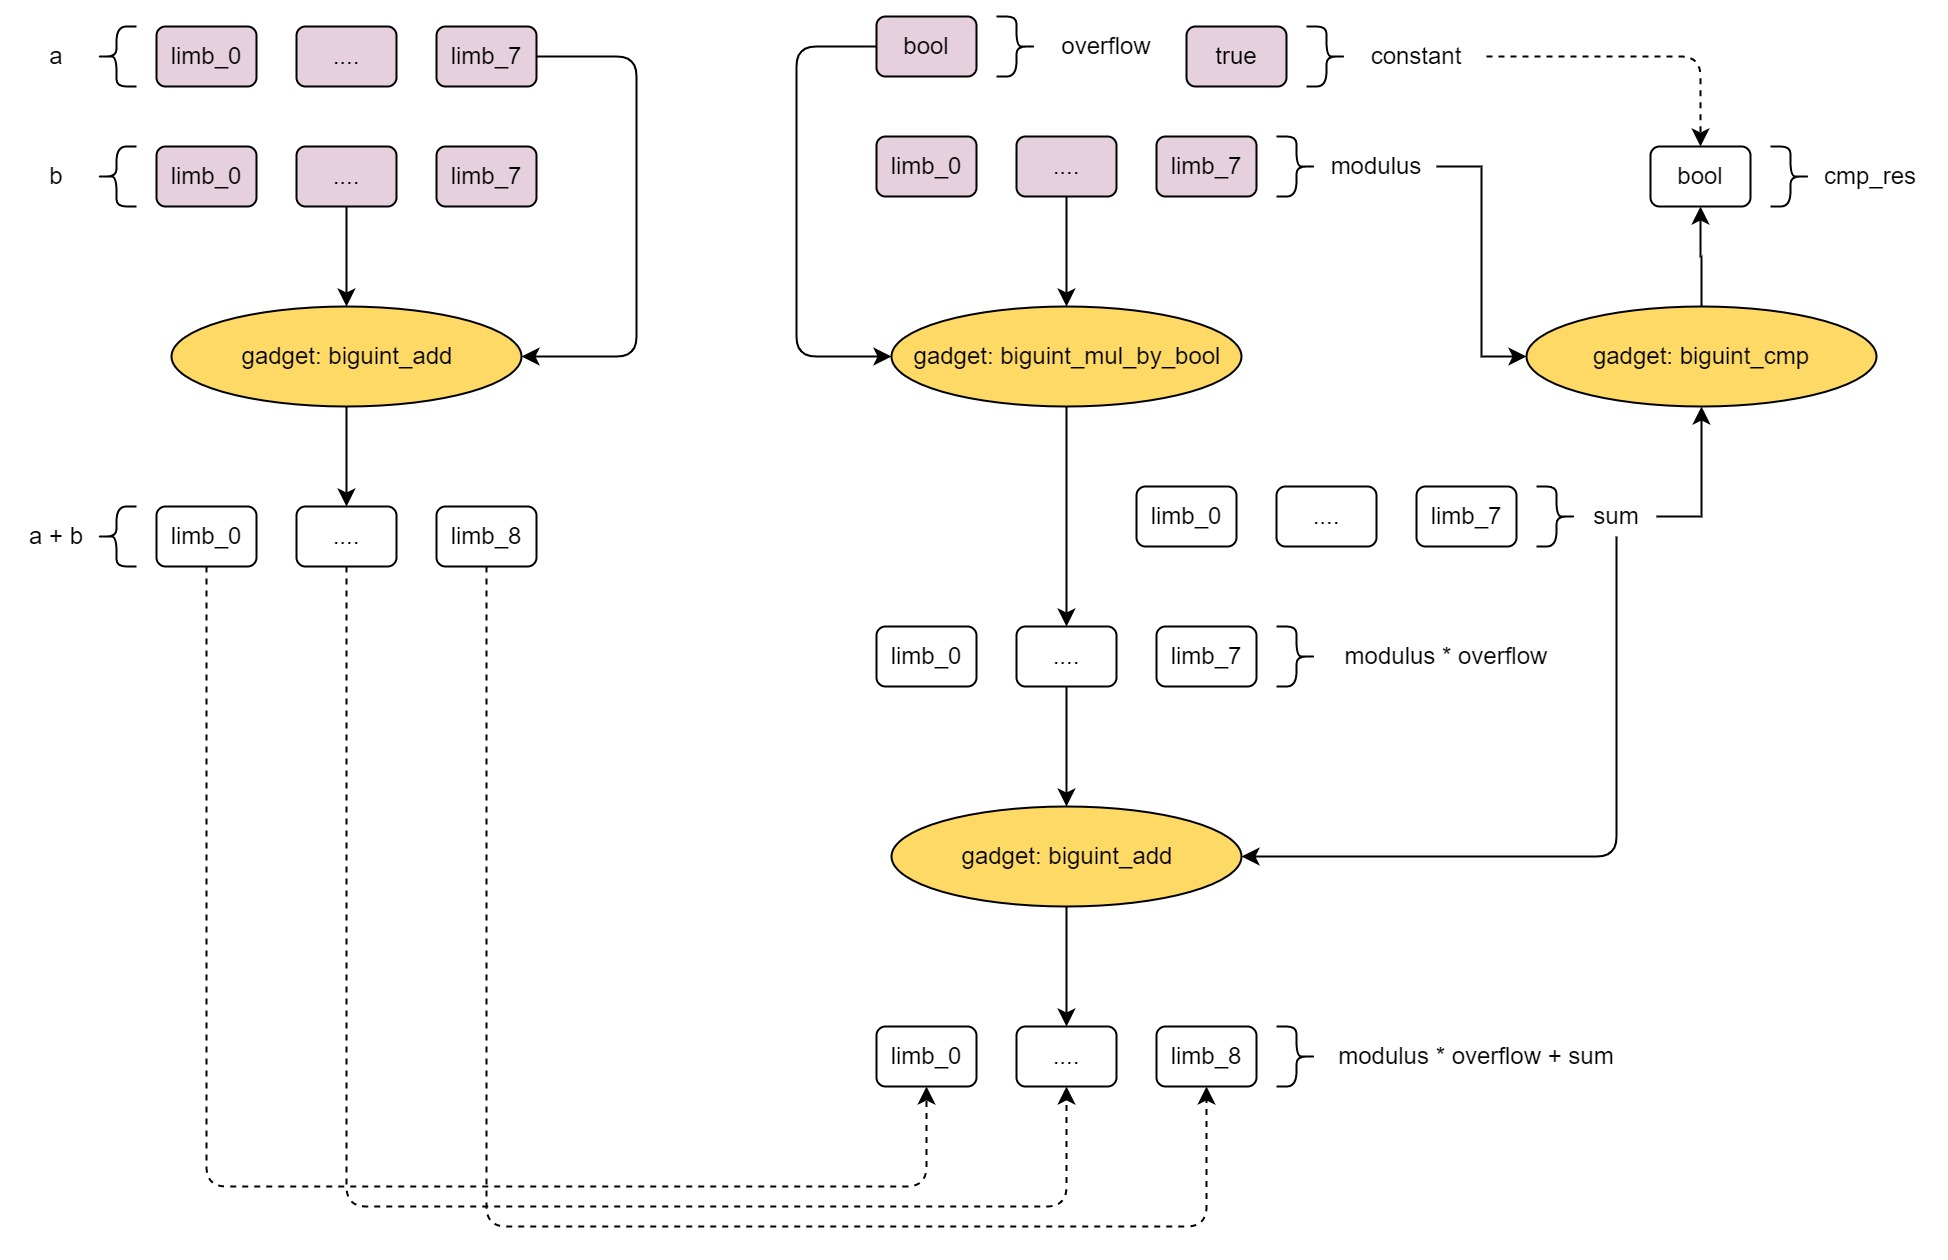
\includegraphics[width=0.8\textwidth]{nonnative-add-layout.jpg}
            \caption{nonnative-add layout}
            \label{fig:nonnative-add-layout}
        \end{figure}
    
    \item constraints-info and costs
        \begin{itemize}
            \item gadget biguint-add num: 2
            \item gadget biguint-mul-by-bool num: 1
            \item gadget biguint-cmp num: 1
            \item gate type num: 3(U32AddManyGate, ComparisonGate, ArithmeticGate)
            \item gate instance num: 23 = 3(U32AddManyGate) + 16(ComparisonGate) + 2(ArithmeticGate(1,0)) + 1(ArithmeticGate(1,-1)) + 1(ArithmeticGate(1,1))
            \item copy-constraints: 186 = 32 * 2{biguint-add} + 9{biguint-mul-by-bool} + 9 + (4 + 9) * 8{biguint-cmp} = 186
        \end{itemize}

    \item questions
        \begin{itemize}
            \item when set value to sum?
        \end{itemize}

\end{enumerate}
    \subsubsection{nonnative-sub}
\label{nonnative-sub}

\begin{enumerate}
    \item target
        check the substract relation among three nonnative target objects.
    \item constraints-logic
        \begin{itemize}
            \item check equation for gadget,  diff + b = a + modular * overflow
            \item check that "overflow is bool"
            \item check that "diff.limbs is range U32"
        \end{itemize}
    \item nonnative-sub process layout
        \begin{figure}[!ht]
            \centering
            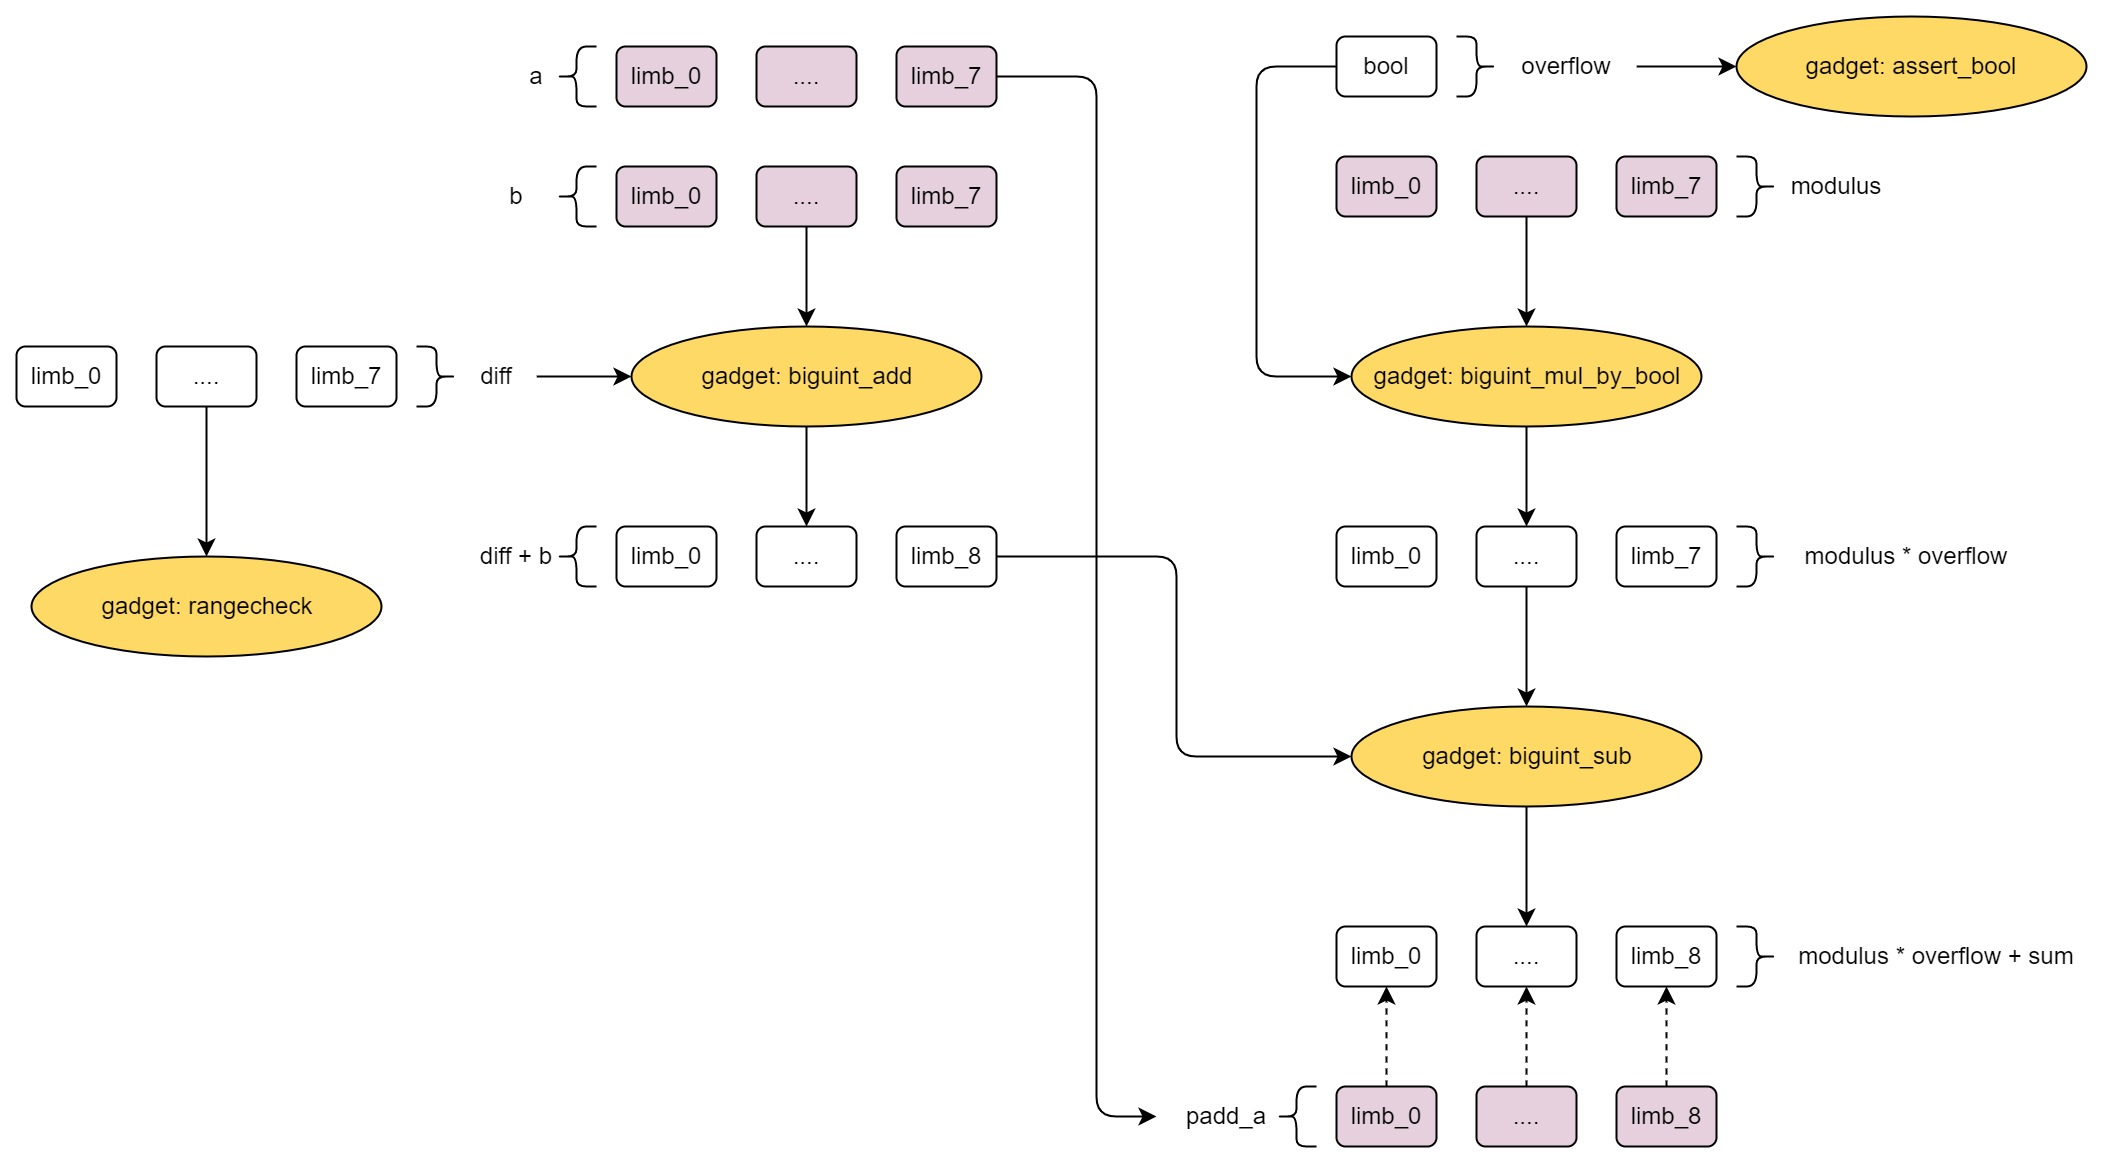
\includegraphics[width=0.8\textwidth]{nonnative-sub-layout.jpg}
            \caption{nonnative-sub layout}
            \label{fig:nonnative-sub-layout}
        \end{figure}
    
    \item constraints-info and costs
        \begin{itemize}
            \item gadget biguint-add num: 1
            \item gadget biguint-sub num: 1
            \item gadget biguint-mul-by-bool num: 1
            \item gadget u32rangecheck num: 1
            \item gadget assert-bool num: 1
            \item gate type num: 4(U32AddManyGate, U32SubtractionGate, U32RangeCheckGate, ArithmeticGate)
            \item gate instance num: 7 = 2(U32AddManyGate) + 2(U32SubtractionGate) + 1(U32RangeCheckGate) + 1(ArithmeticGate(1,0)) + 1(ArithmeticGate(1,-1))
            \item copy-constraints: 89 = 32{biguint-add num} + 27{U32SubtractionGate} + 9{biguint-mul-by-bool} + 8{u32rangecheck} + 4{assert-bool} + 9
        \end{itemize}

    \item questions
        \begin{itemize}
            \item why not constraint for overflow at nonnative-add?
            \item why not make u32rangecheck for input at nonnative-add?
        \end{itemize}

\end{enumerate}
    \subsubsection{nonnative-mul}
\label{nonnative-mul}

\begin{enumerate}
    \item target
        check the multiplicatipn relation among three nonnative target objects.
    \item constraints-logic
        \begin{itemize}
            \item check equation for gadget,  a * b = prod + modular * overflow
            \item check that "overflow.limb is U32"
            \item check that "prod.limb is U32"
        \end{itemize}
    \item nonnative-mul process layout
        \begin{figure}[!ht]
            \centering
            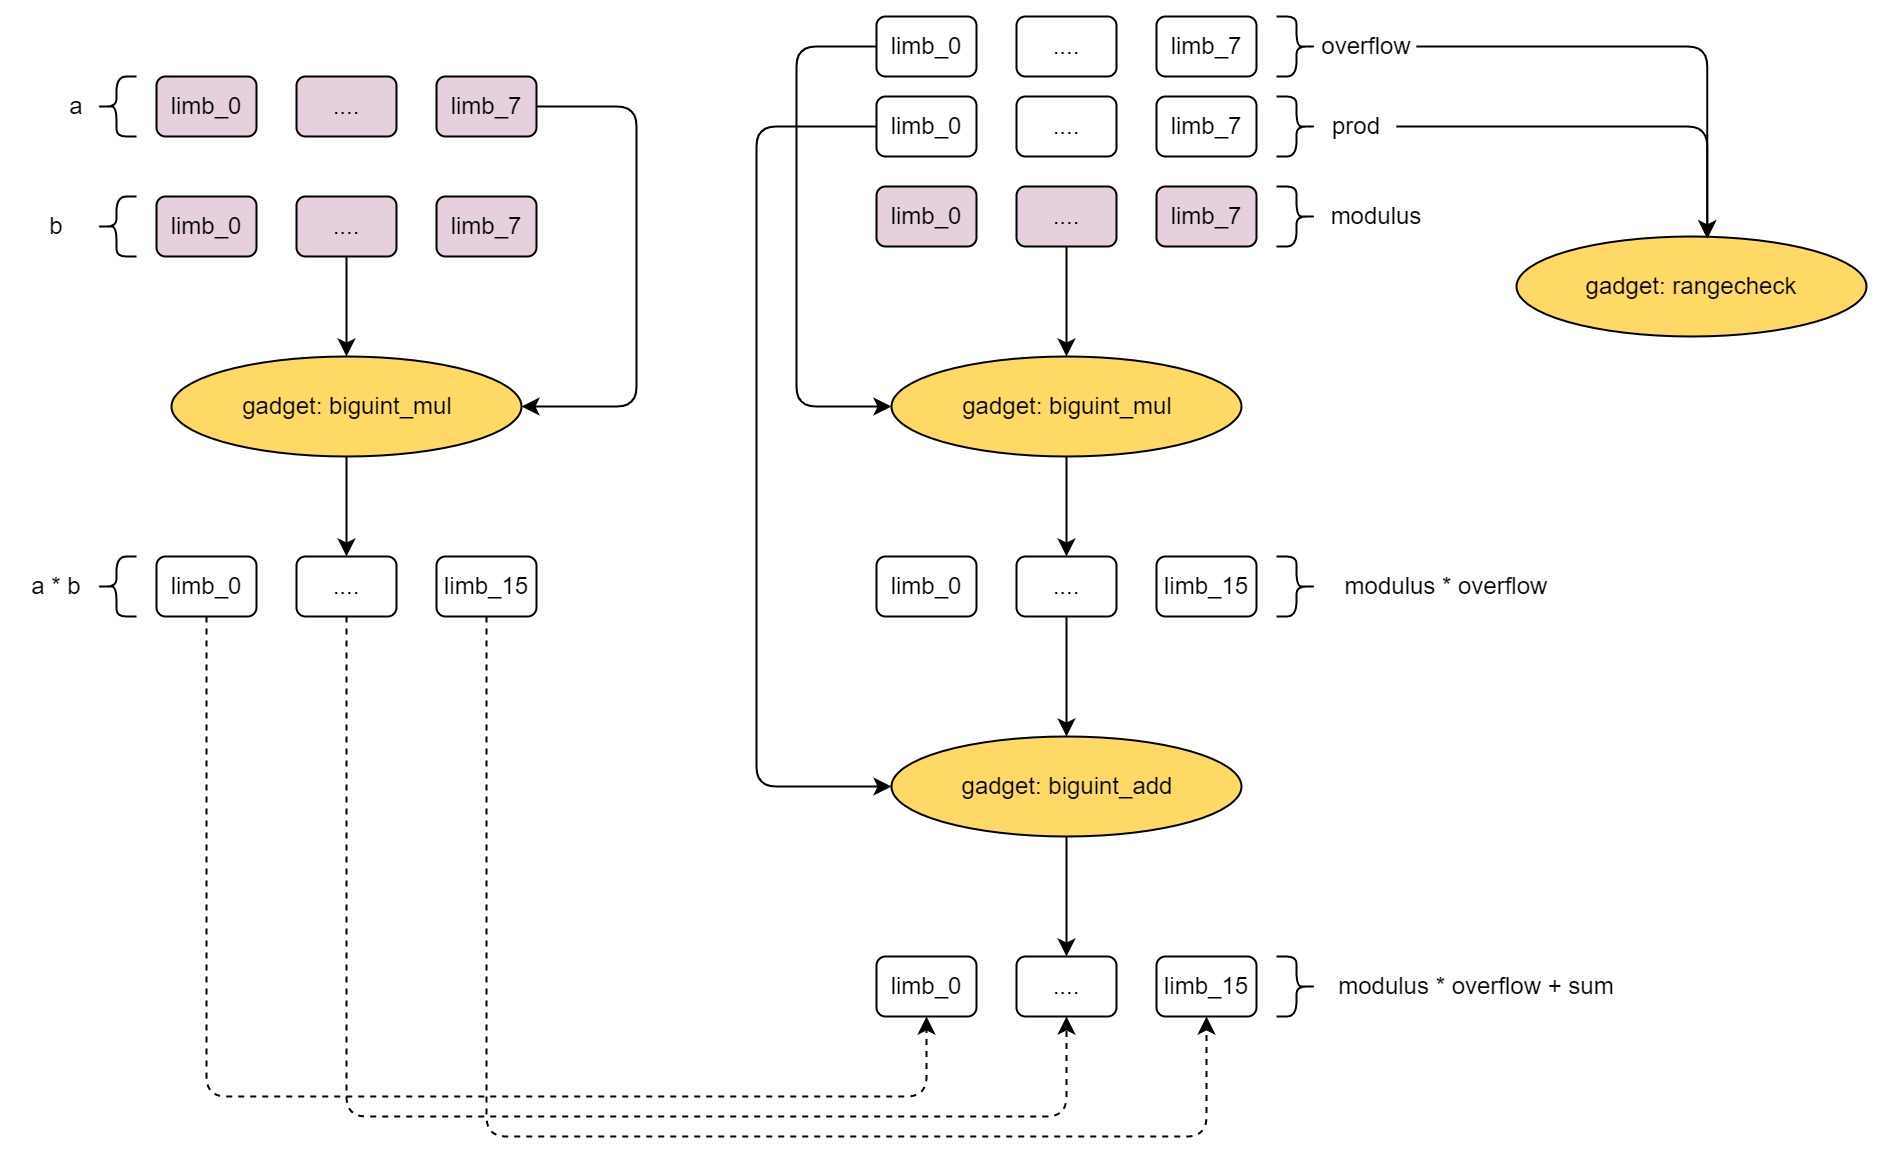
\includegraphics[width=0.8\textwidth]{nonnative-mul-layout.jpg}
            \caption{nonnative-mul layout}
            \label{fig:nonnative-mul-layout}
        \end{figure}
    
    \item constraints-info and costs
        \begin{itemize}
            \item gadget biguint-add num: 1
            \item gadget biguint-mul num: 2
            \item gadget u32rangecheck num: 2
            \item gate type num: 9 = 7(U32AddManyGate{3,5,7,9,11,13,15}) + 1(U32RangeCheckGate) + 1(U32ArithmeticGate)
            \item gate instance num: 37 = 2(u32rangecheck) + 8(biguint-mul: constant-input) + 22(biguint-mul) + 1 + 3(biguint-add)
            \item copy-constraints: 583 = 8 * 2(u32rangecheck) + 3 * 3 + (4 + 6 + 8 + 10 + 12 + 14 + 16) * 4 + (8 * 8) * 3 + 17 * 4 + 18
        \end{itemize}

\end{enumerate}
    \subsubsection{nonnative-inv}

\Par{Target}
Check the modular inverse relation among three nonnative target objects.

\Par{Constraints logic}
\begin{itemize}
    \item Check equation for gadget: \verb|a * inv_a = 1 + modular * div|.
\end{itemize}

\Par{Process layout}
See \figref{fig:nonnative-inv-layout}.
\begin{figure}[!ht]
    \centering
    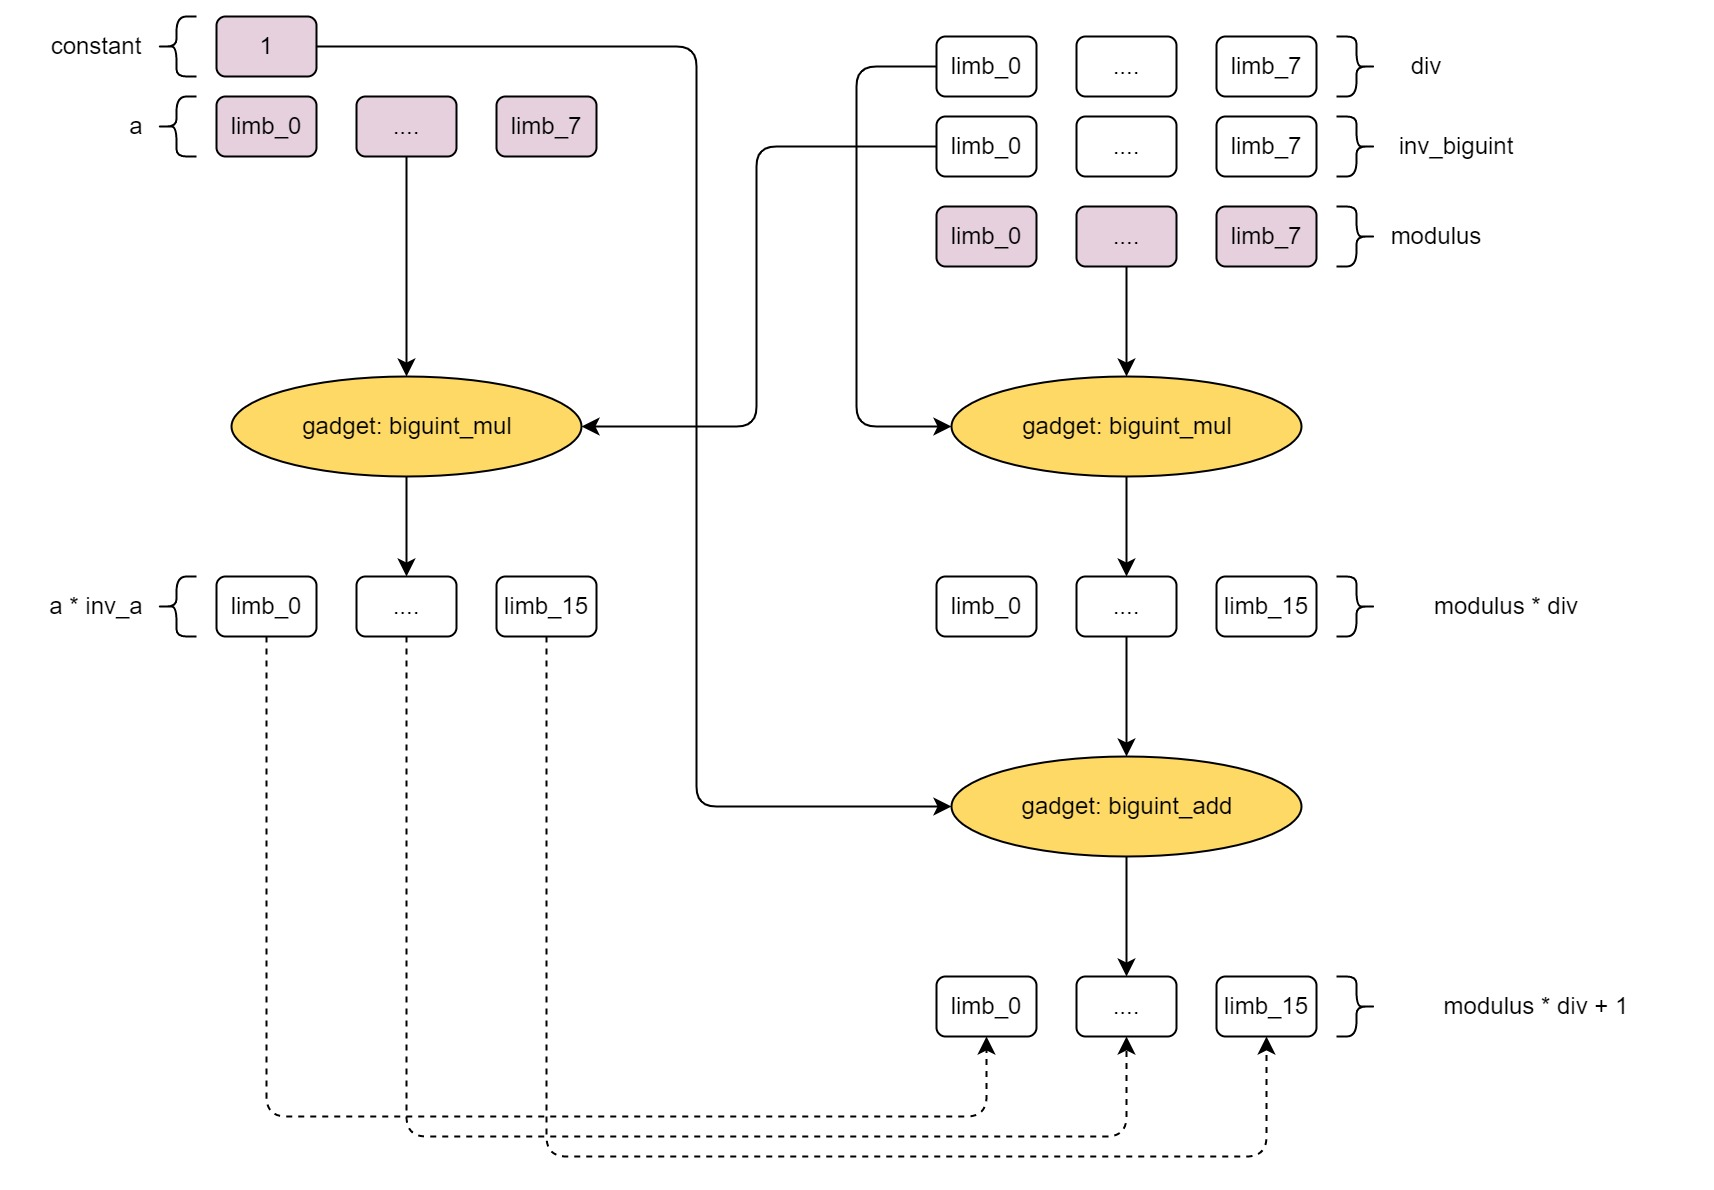
\includegraphics[width=0.8\textwidth]{nonnative-inv-layout.jpg}
    \caption{nonnative-inv layout}
    \label{fig:nonnative-inv-layout}
\end{figure}

\Par{Constraints info and costs}
\begin{itemize}
    \item gadget biguint-add num: 1
    \item gadget biguint-mul num: 2
    \item gate type num: 8 = 7(U32AddManyGate\{3,5,7,9,11,13,15\}) + 1(U32ArithmeticGate)
    \item gate instance num: 56 = (8 * 8 + 2) * 2 / 3 + 5(U32AddManyGate{3}) + 5 + 2(U32AddManyGate{15})
    \item copy-constraints: 762 = (8 * 8 + 2) * 2 * 3 + 21 * 4 + (6 + 8 + 10 + 12 + 14) * 4 + 4 * 16 + 18
\end{itemize}

    \section{curve-add}
\label{curve-add}

Take curve-secp256k1 as example, the same as other texs.

\begin{enumerate}
    \item target
        implement the addition of two different curve points. this is a incomplete addition, you can refer to The halo2 Book \cite{website:halo2-book} to learn more about it.
    \item constraints-logic
        \begin{figure}[!ht]
            \centering
            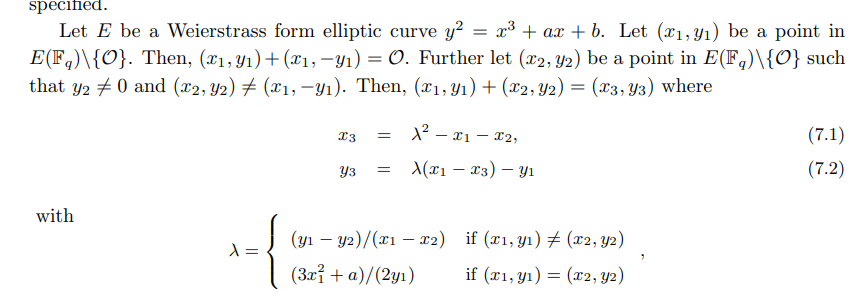
\includegraphics[width=0.8\textwidth]{curve-add.jpg}
            \caption{curve-add}
            \label{fig:curve-add}
        \end{figure}
    \item curve-add process layout
        \begin{figure}[!ht]
            \centering
            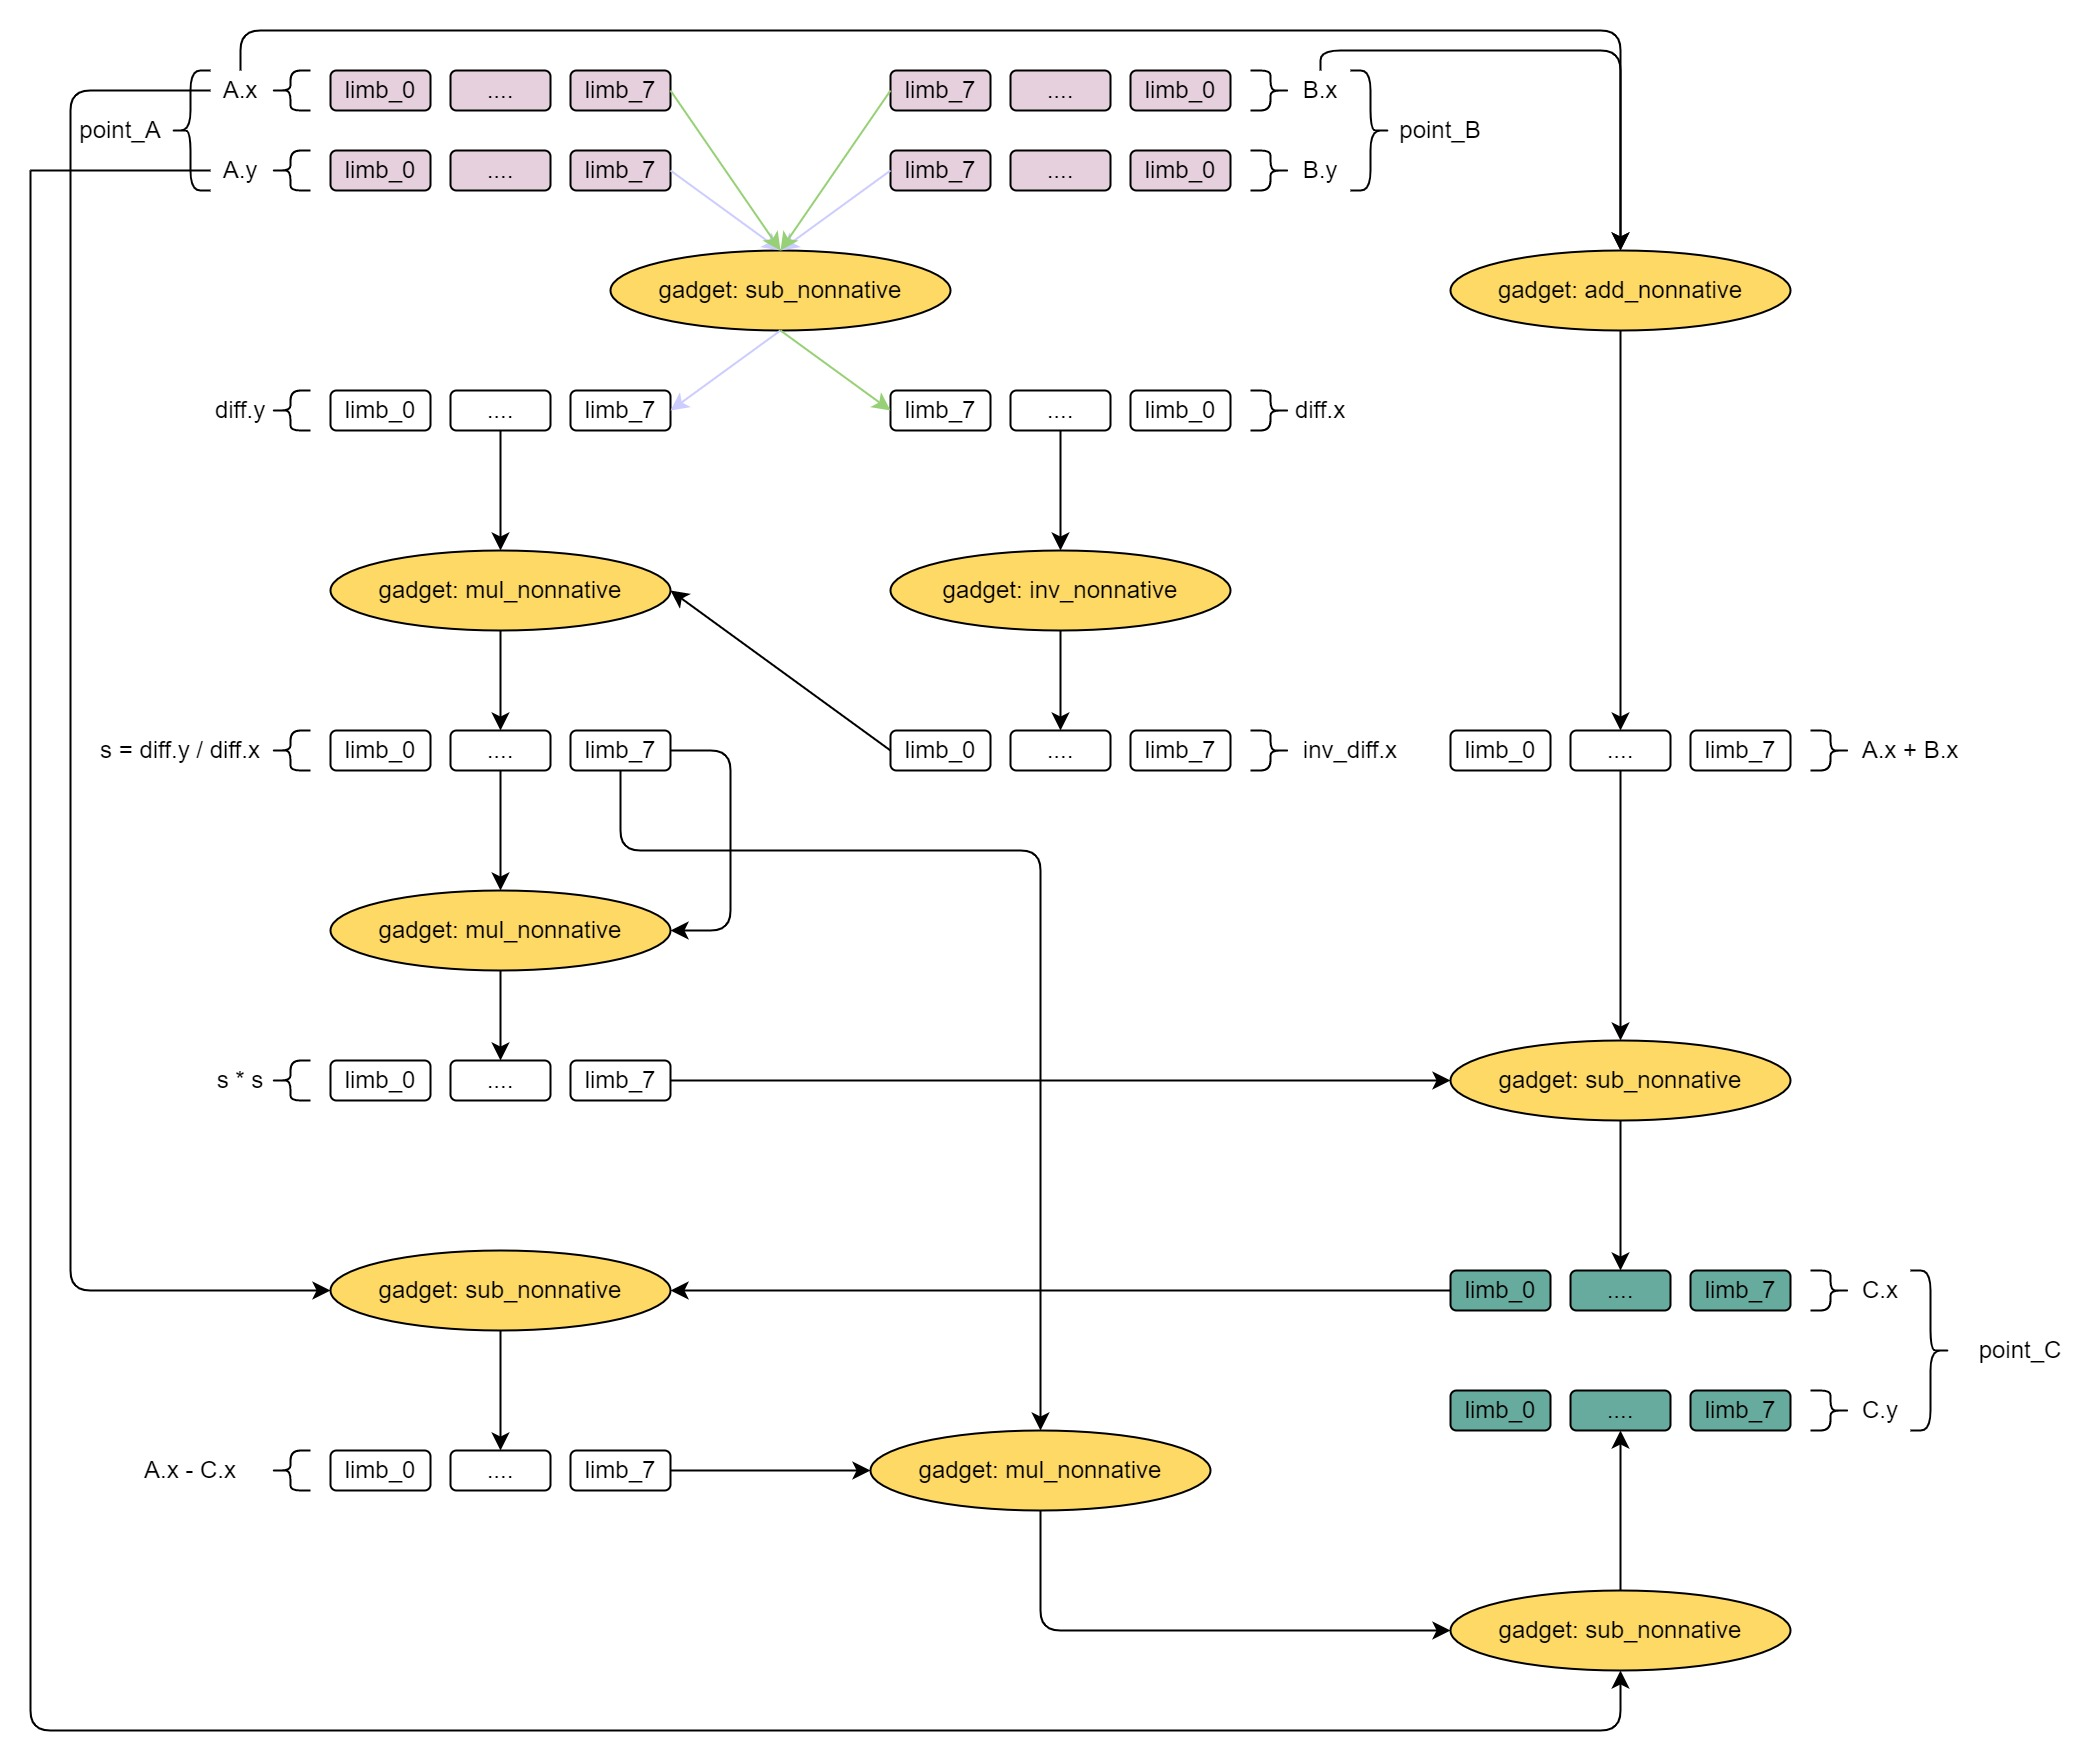
\includegraphics[width=0.8\textwidth]{curve-add-layout.jpg}
            \caption{curve-add layout}
            \label{fig:curve-add-layout}
        \end{figure}
    
    \item constraints-info and costs
        \begin{itemize}
            \item gadget-sub-nonnative num: 5
            \item gadget-add-nonnative num: 1
            \item gadget-mul-nonnative num: 3
            \item gadget-inv-nonnative num: 1
            \item gate type num: 
            \item gate instance num: 
        \end{itemize}

\end{enumerate}
    %\printbibliography[heading=bibintoc, title=\ebibname]%
\end{document}

    \subsubsection{biguint-add}

\Par{Target}
Implement the addition of two biguints.

\Par{Constraints logic}
\begin{itemize}
    \item Equation for gates;
    \item Sumcheck between output and limbs;
    \item Rangecheck for limbs.
\end{itemize}

\Par{Circuit layout}
See \figref{fig:biguint-add-circuit-layout}.
\begin{figure}[!ht]
    \centering
    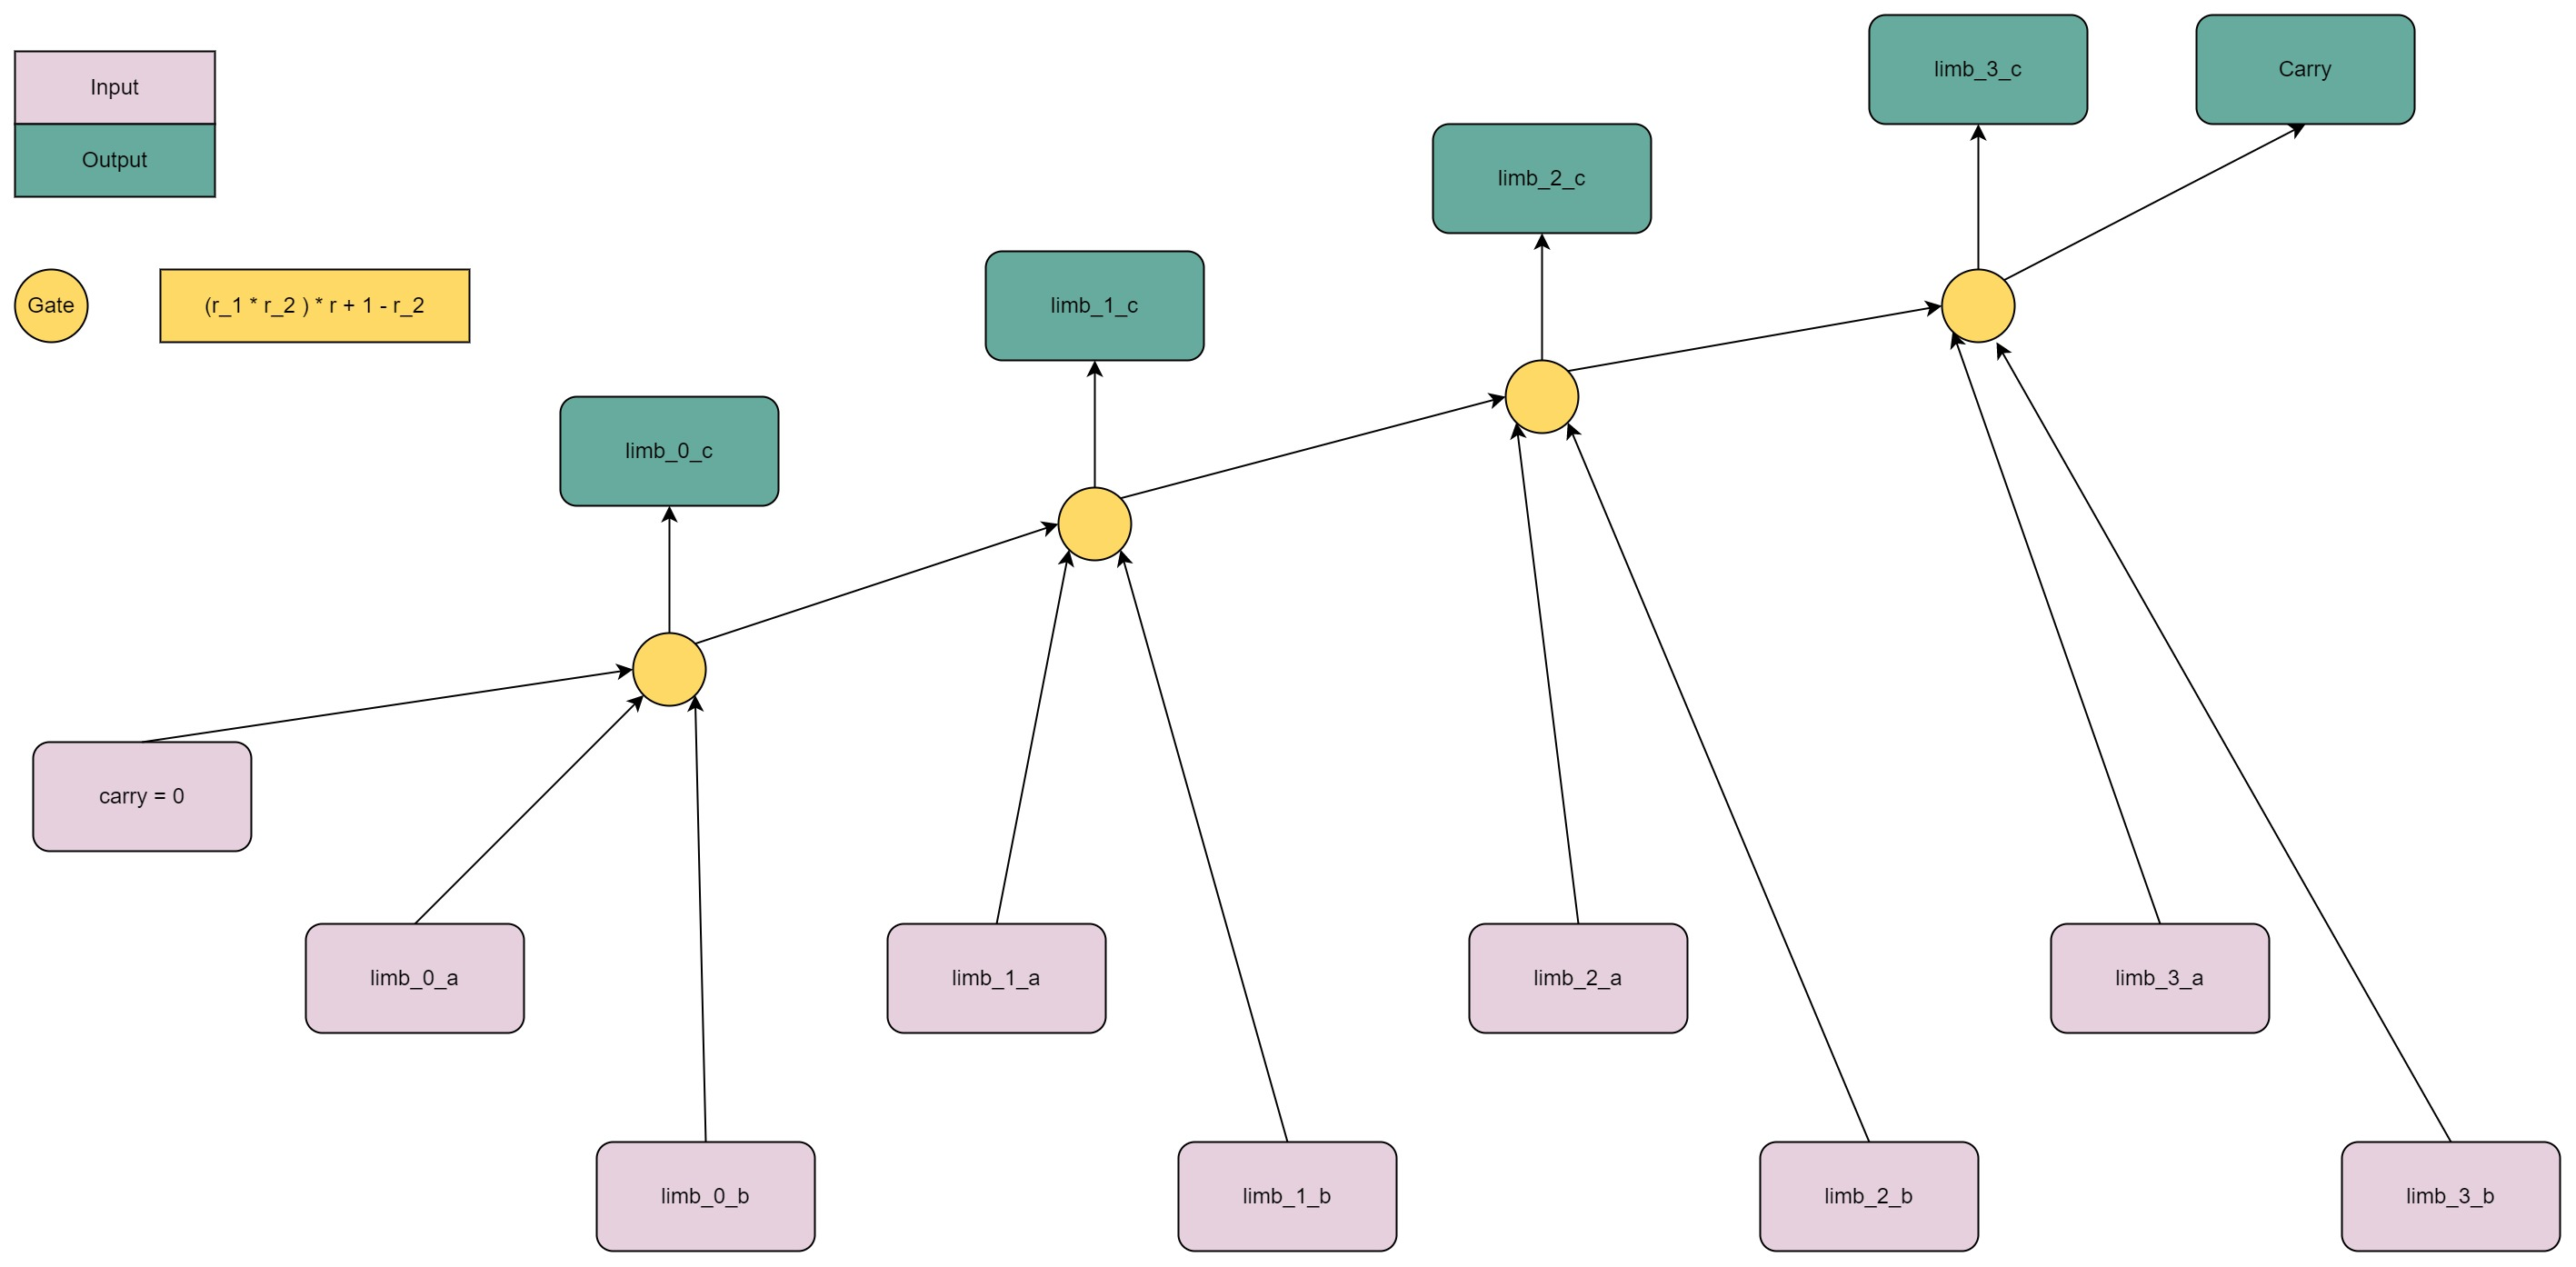
\includegraphics[width=0.8\textwidth]{biguint-add-circuit-layout.jpg}
    \caption{biguint-add circuit layout}
    \label{fig:biguint-add-circuit-layout}
\end{figure}

\Par{Trace layout}
See \figref{fig:biguint-add-trace-layout}.
\begin{figure}[!ht]
    \centering
    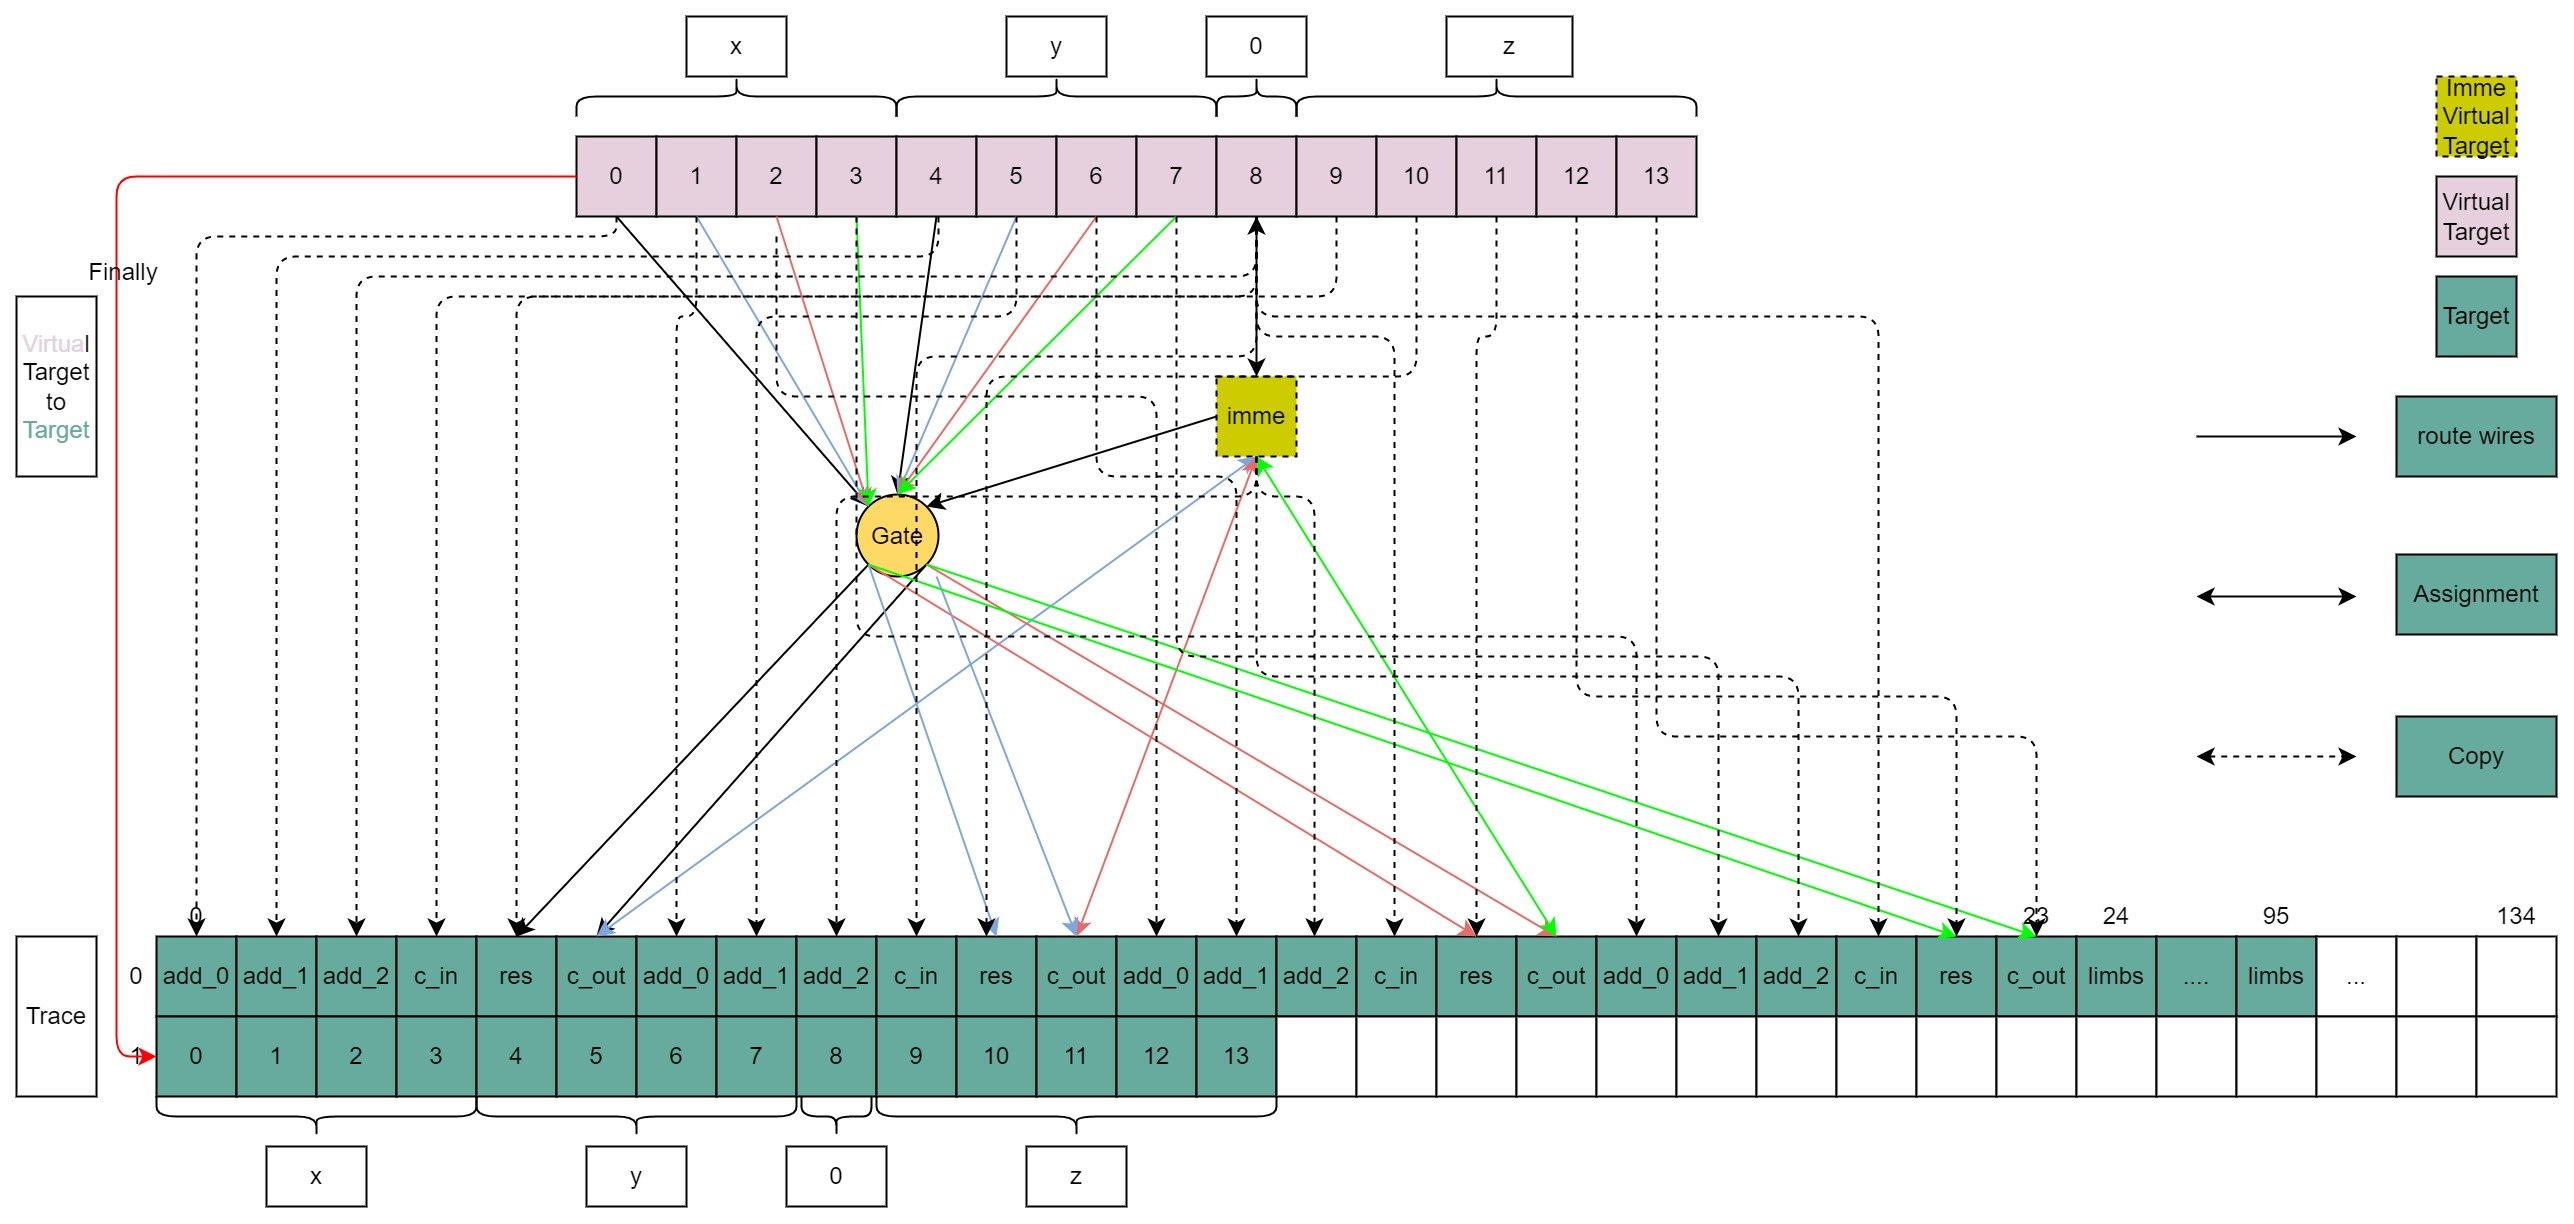
\includegraphics[width=0.8\textwidth]{biguint-add-trace-layout.jpg}
    \caption{biguint-add trace layout}
    \label{fig:biguint-add-trace-layout}
\end{figure}

\Par{Constraints info and costs}
\begin{itemize}
    \item gate type num: 1 (U32AddManyGate)
    \item gate ops num: limbs-num
    \item gate instance num: ceil(limbs-num / gate.ops)
    \item copy-constraints: limbs-num * 4
    \item max-degree: 4 (\verb|1 << limb-bits|)
\end{itemize}

\Par{Questions}
\begin{itemize}
    \item Why not make rangecheck constraint for inputs?
    \item Why not make copy constraint between cur-c-in and last-c-out?
\end{itemize}

    \subsubsection{biguint-sub}

\Par{Target}
Implement the substraction of two biguints.

\Par{Constraints logic}
\begin{itemize}
    \item Equation for gate;
    \item Sumcheck for ouptput;
    \item Rangecheck for limbs.
\end{itemize}

\Par{Circuit layout}
See \figref{fig:biguint-sub-circuit-layout}.
\begin{figure}[!ht]
    \centering
    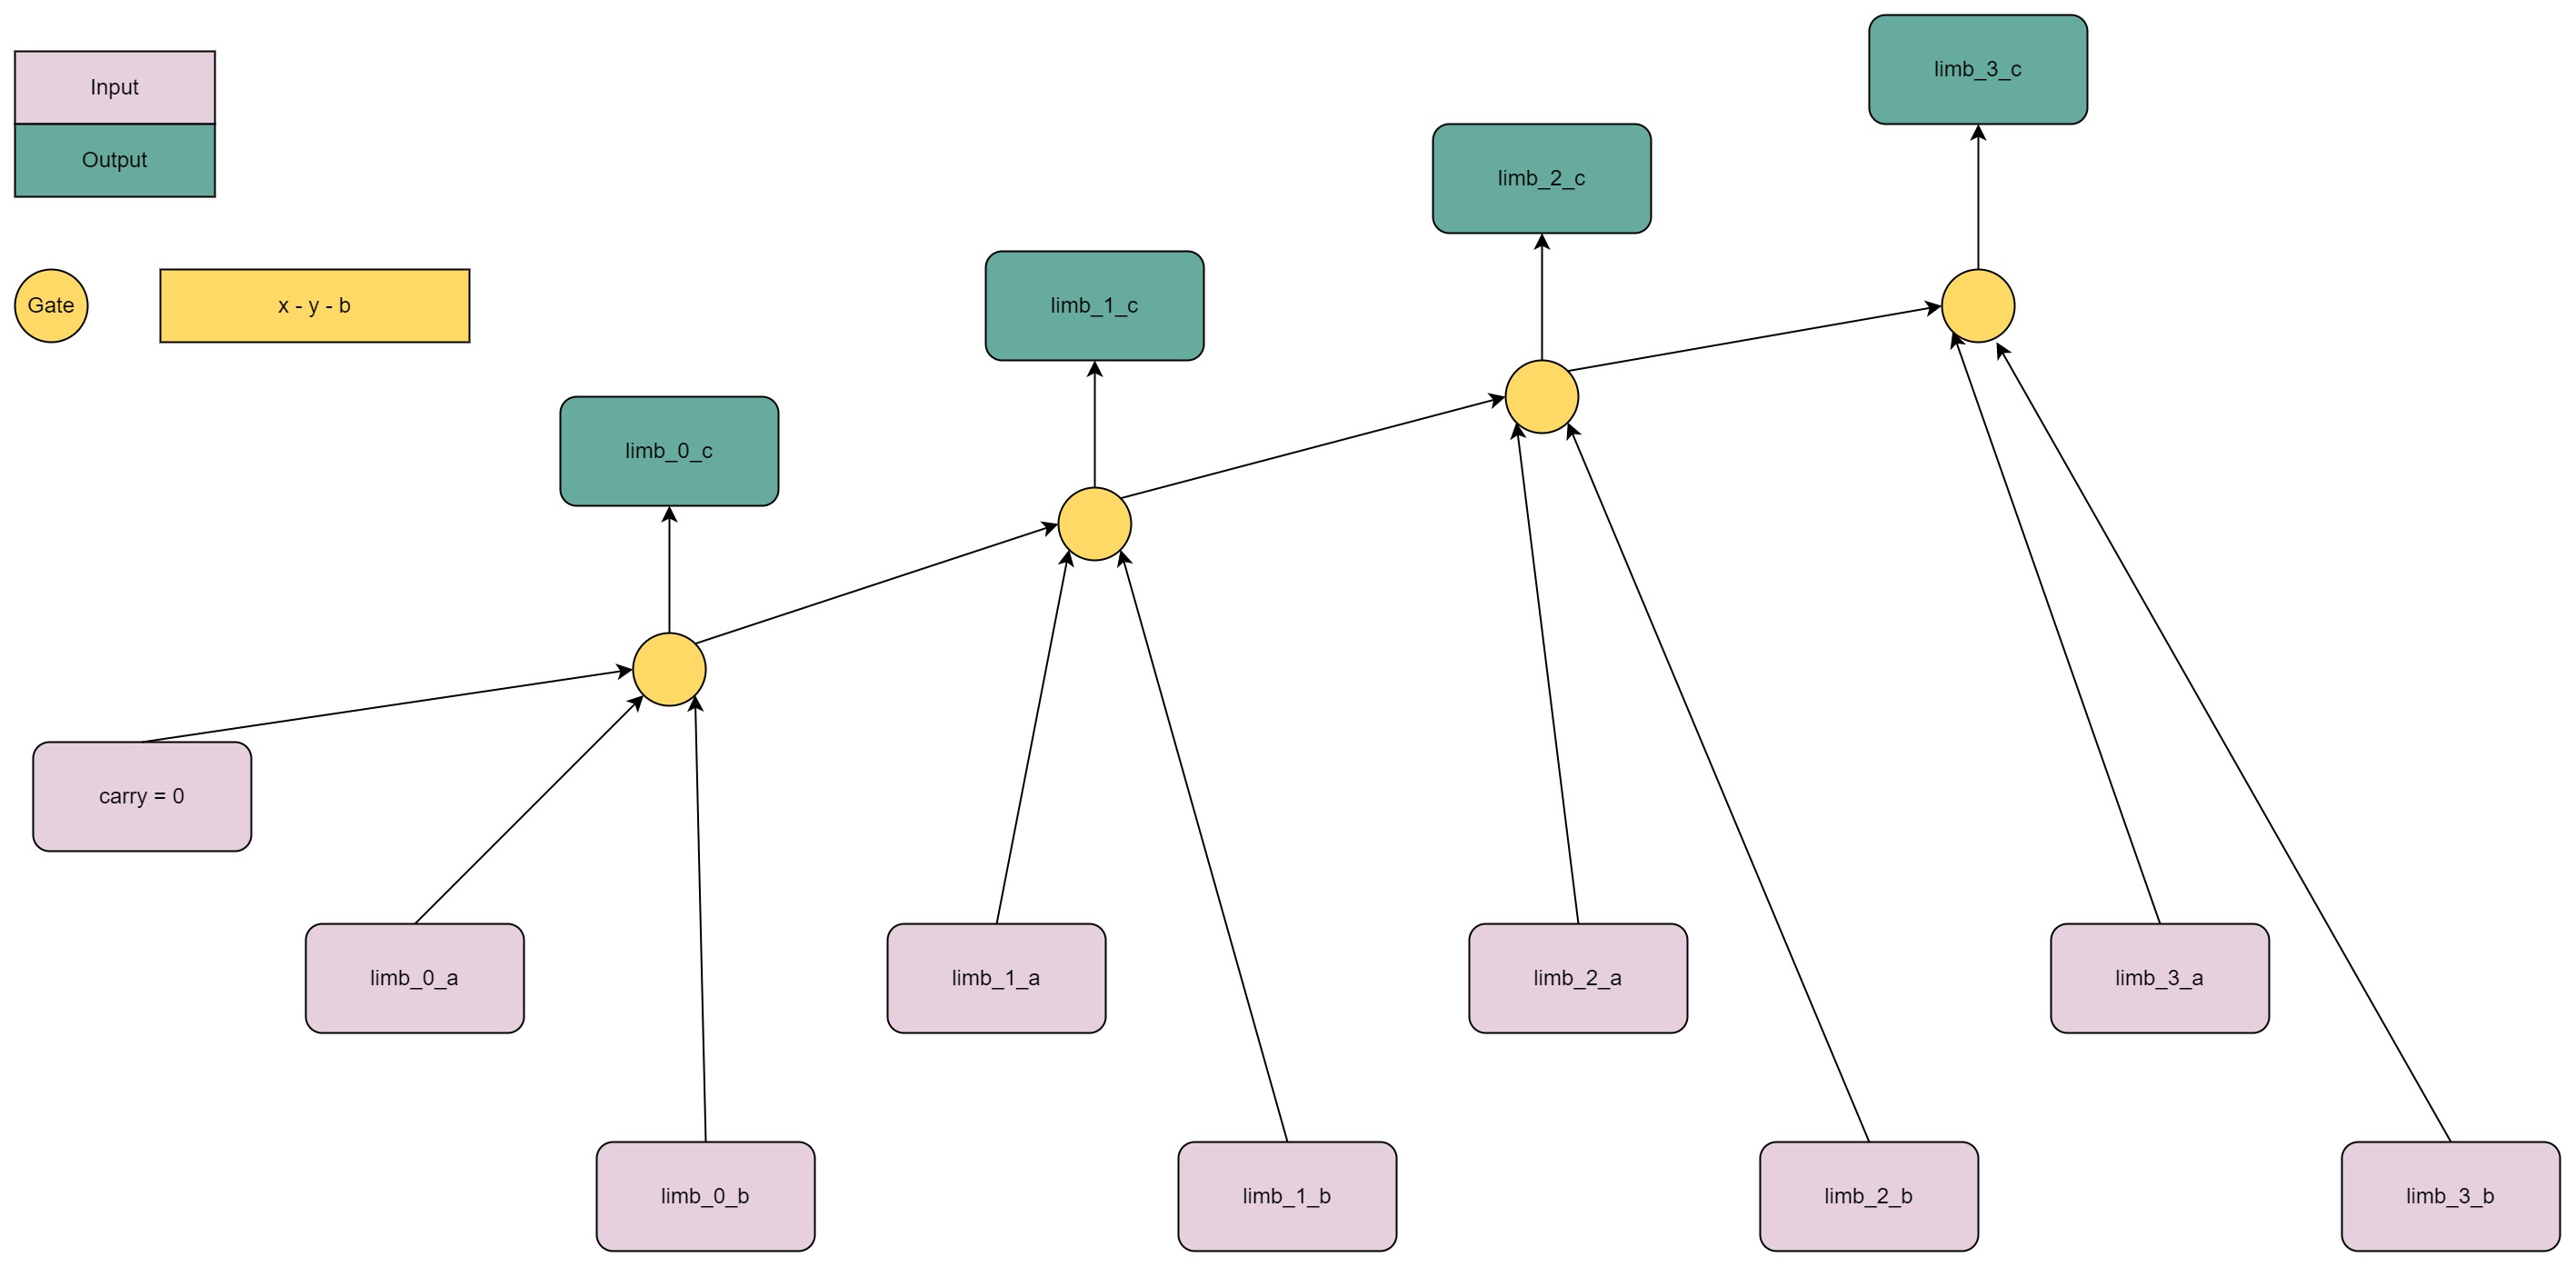
\includegraphics[width=0.8\textwidth]{biguint-sub-circuit-layout.jpg}
    \caption{biguint-sub circuit layout}
    \label{fig:biguint-sub-circuit-layout}
\end{figure}

\Par{Trace layout}
See \figref{fig:biguint-sub-trace-layout}.
\begin{figure}[!ht]
    \centering
    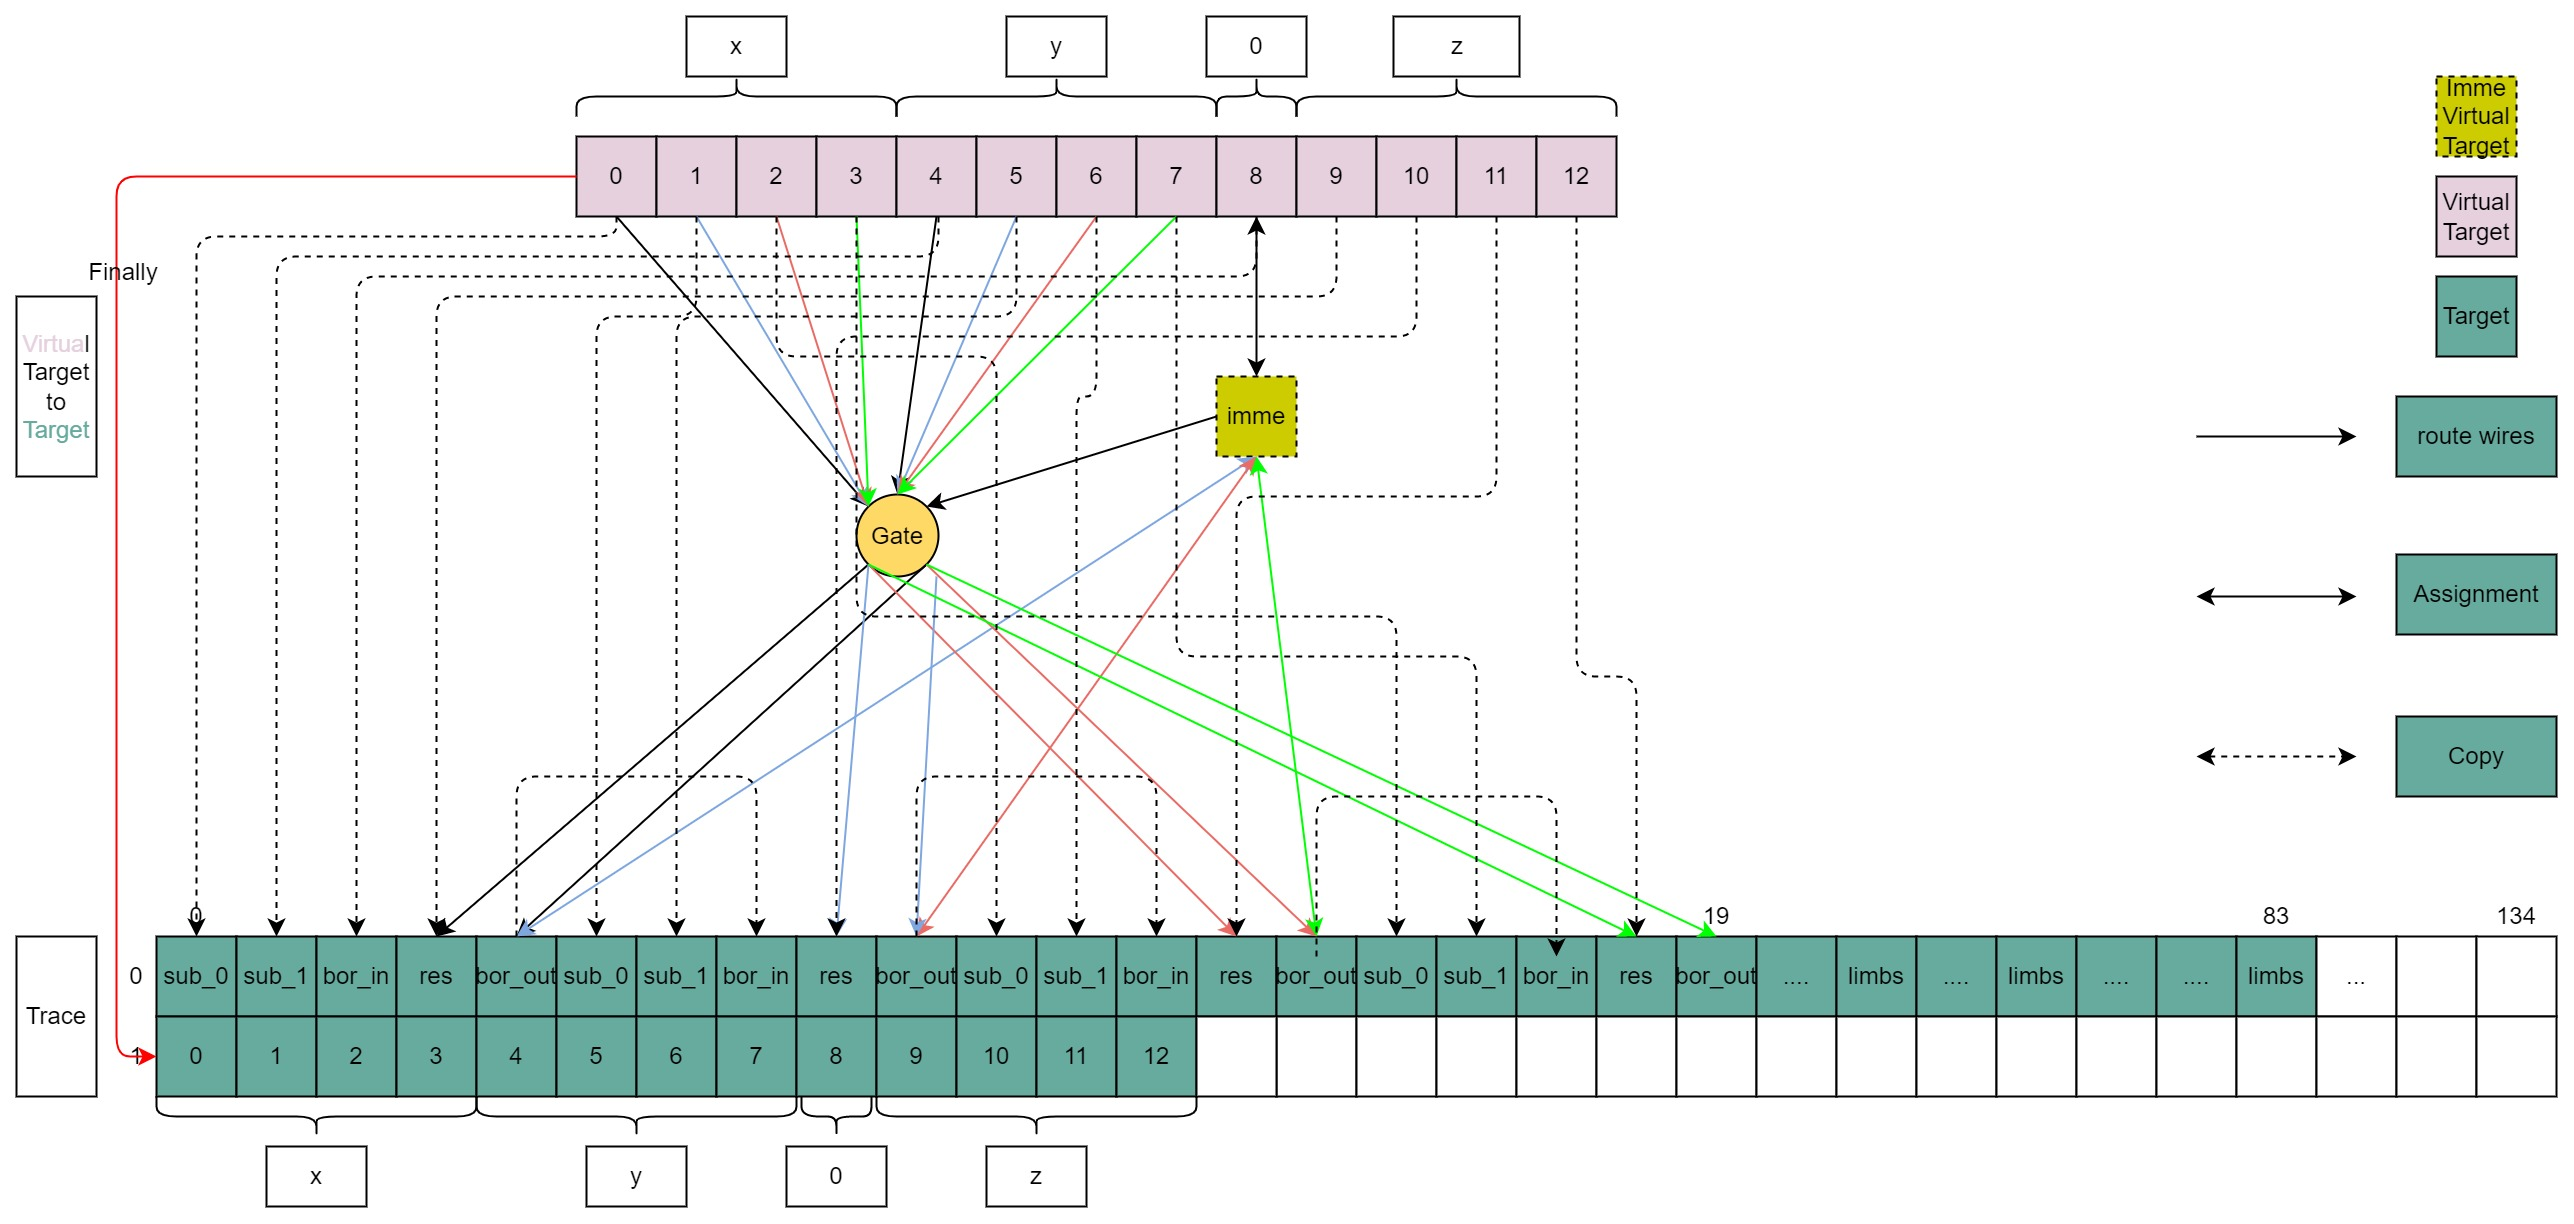
\includegraphics[width=0.8\textwidth]{biguint-sub-trace-layout.jpg}
    \caption{biguint-sub trace layout}
    \label{fig:biguint-sub-trace-layout}
\end{figure}

\Par{Constraints info and costs}
\begin{itemize}
    \item constraints-num: $6 \times (3 + 32 / 2) = 114$
    \item copy-constraints: $16$
    \item max-degree: $4$
    \item wires-num: $6 \times (5 + 16) = 126$
\end{itemize}

\Par{Questions}
\begin{itemize}
    \item Why not make rangecheck constraint for inputs?
    \item Could try to use the same constraint with add-gate.
\end{itemize}

    \subsubsection{biguint-mul}

\Par{Target}
Implement the multiplication of two biguints.

\Par{Constraints logic}
\begin{itemize}
    \item Compute mul-factors first, use U32ArithmeticGate;
    \item Add mul-factors from low bits, use U32AddManyGate.
\end{itemize}

\Par{Process layout}
See \figref{fig:biguint-mul-layout}
\begin{figure}[!ht]
    \centering
    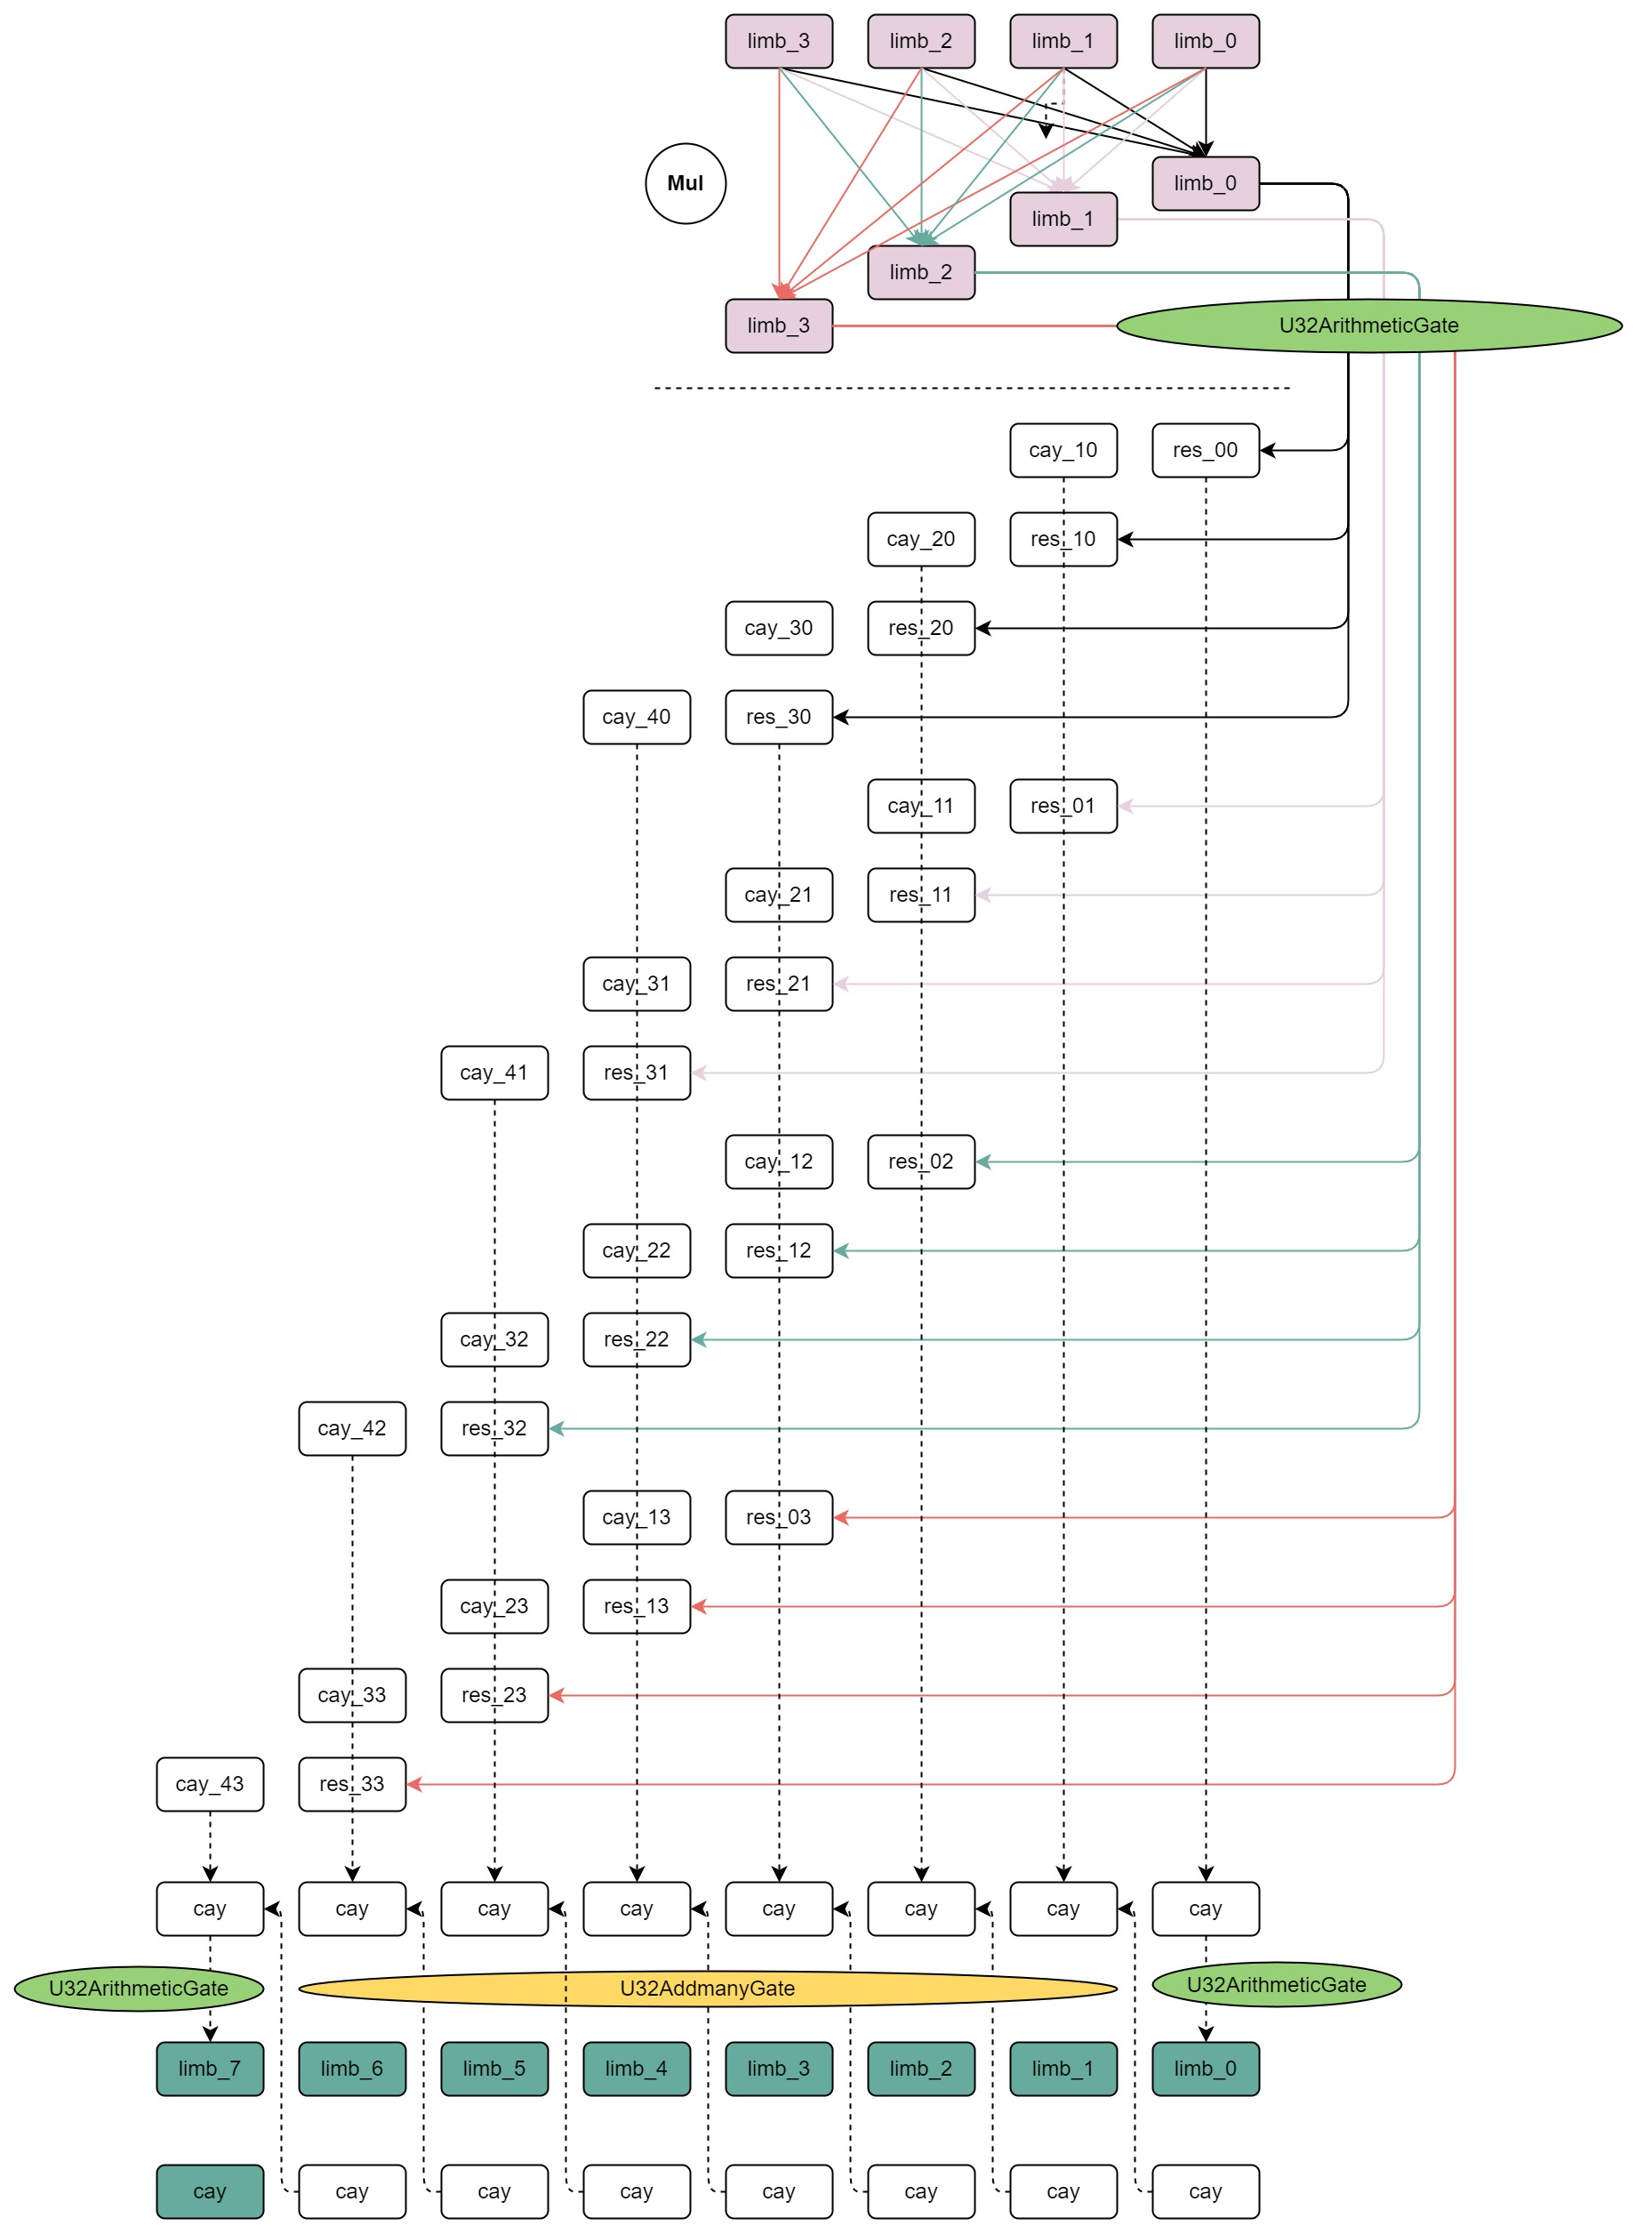
\includegraphics[width=0.8\textwidth]{biguint-mul-layout.jpg}
    \caption{biguint-mul layout}
    \label{fig:biguint-mul-layout}
\end{figure}

\Par{Constraints info and costs}
\begin{itemize}
    \item Gate type num: 4 (U32ArithmeticGate, U32AddManyGate(num-addends: 4), U32AddManyGate(num-addends: 6), U32AddManyGate(num-addends: 8))
    \item Gate instance num: 9
    \item U32ArithmeticGate num: 6
    \item U32AddManyGate num: 3
    \item copy-constraints: $18 \times 3 + (4 + 6 + 8) \times 2 + 9 = 99$
    \item max-degree: 4
\end{itemize}

    \section{biguint-div}
\label{biguint-div}

Note that div-rem has the same constraints logic with div

\begin{enumerate}
    \item target
        \begin{itemize}
            \item implement the division of two biguints
        \end{itemize}
    \item constraints-logic
        \begin{itemize}
            \item not implement div-algrithem directly
            \item use nondeterministic feature to check div-logic
            \item check div * b + rem = a
            \item check rem < b
        \end{itemize}
    \item div-process layout
        \begin{figure}[!ht]
            \centering
            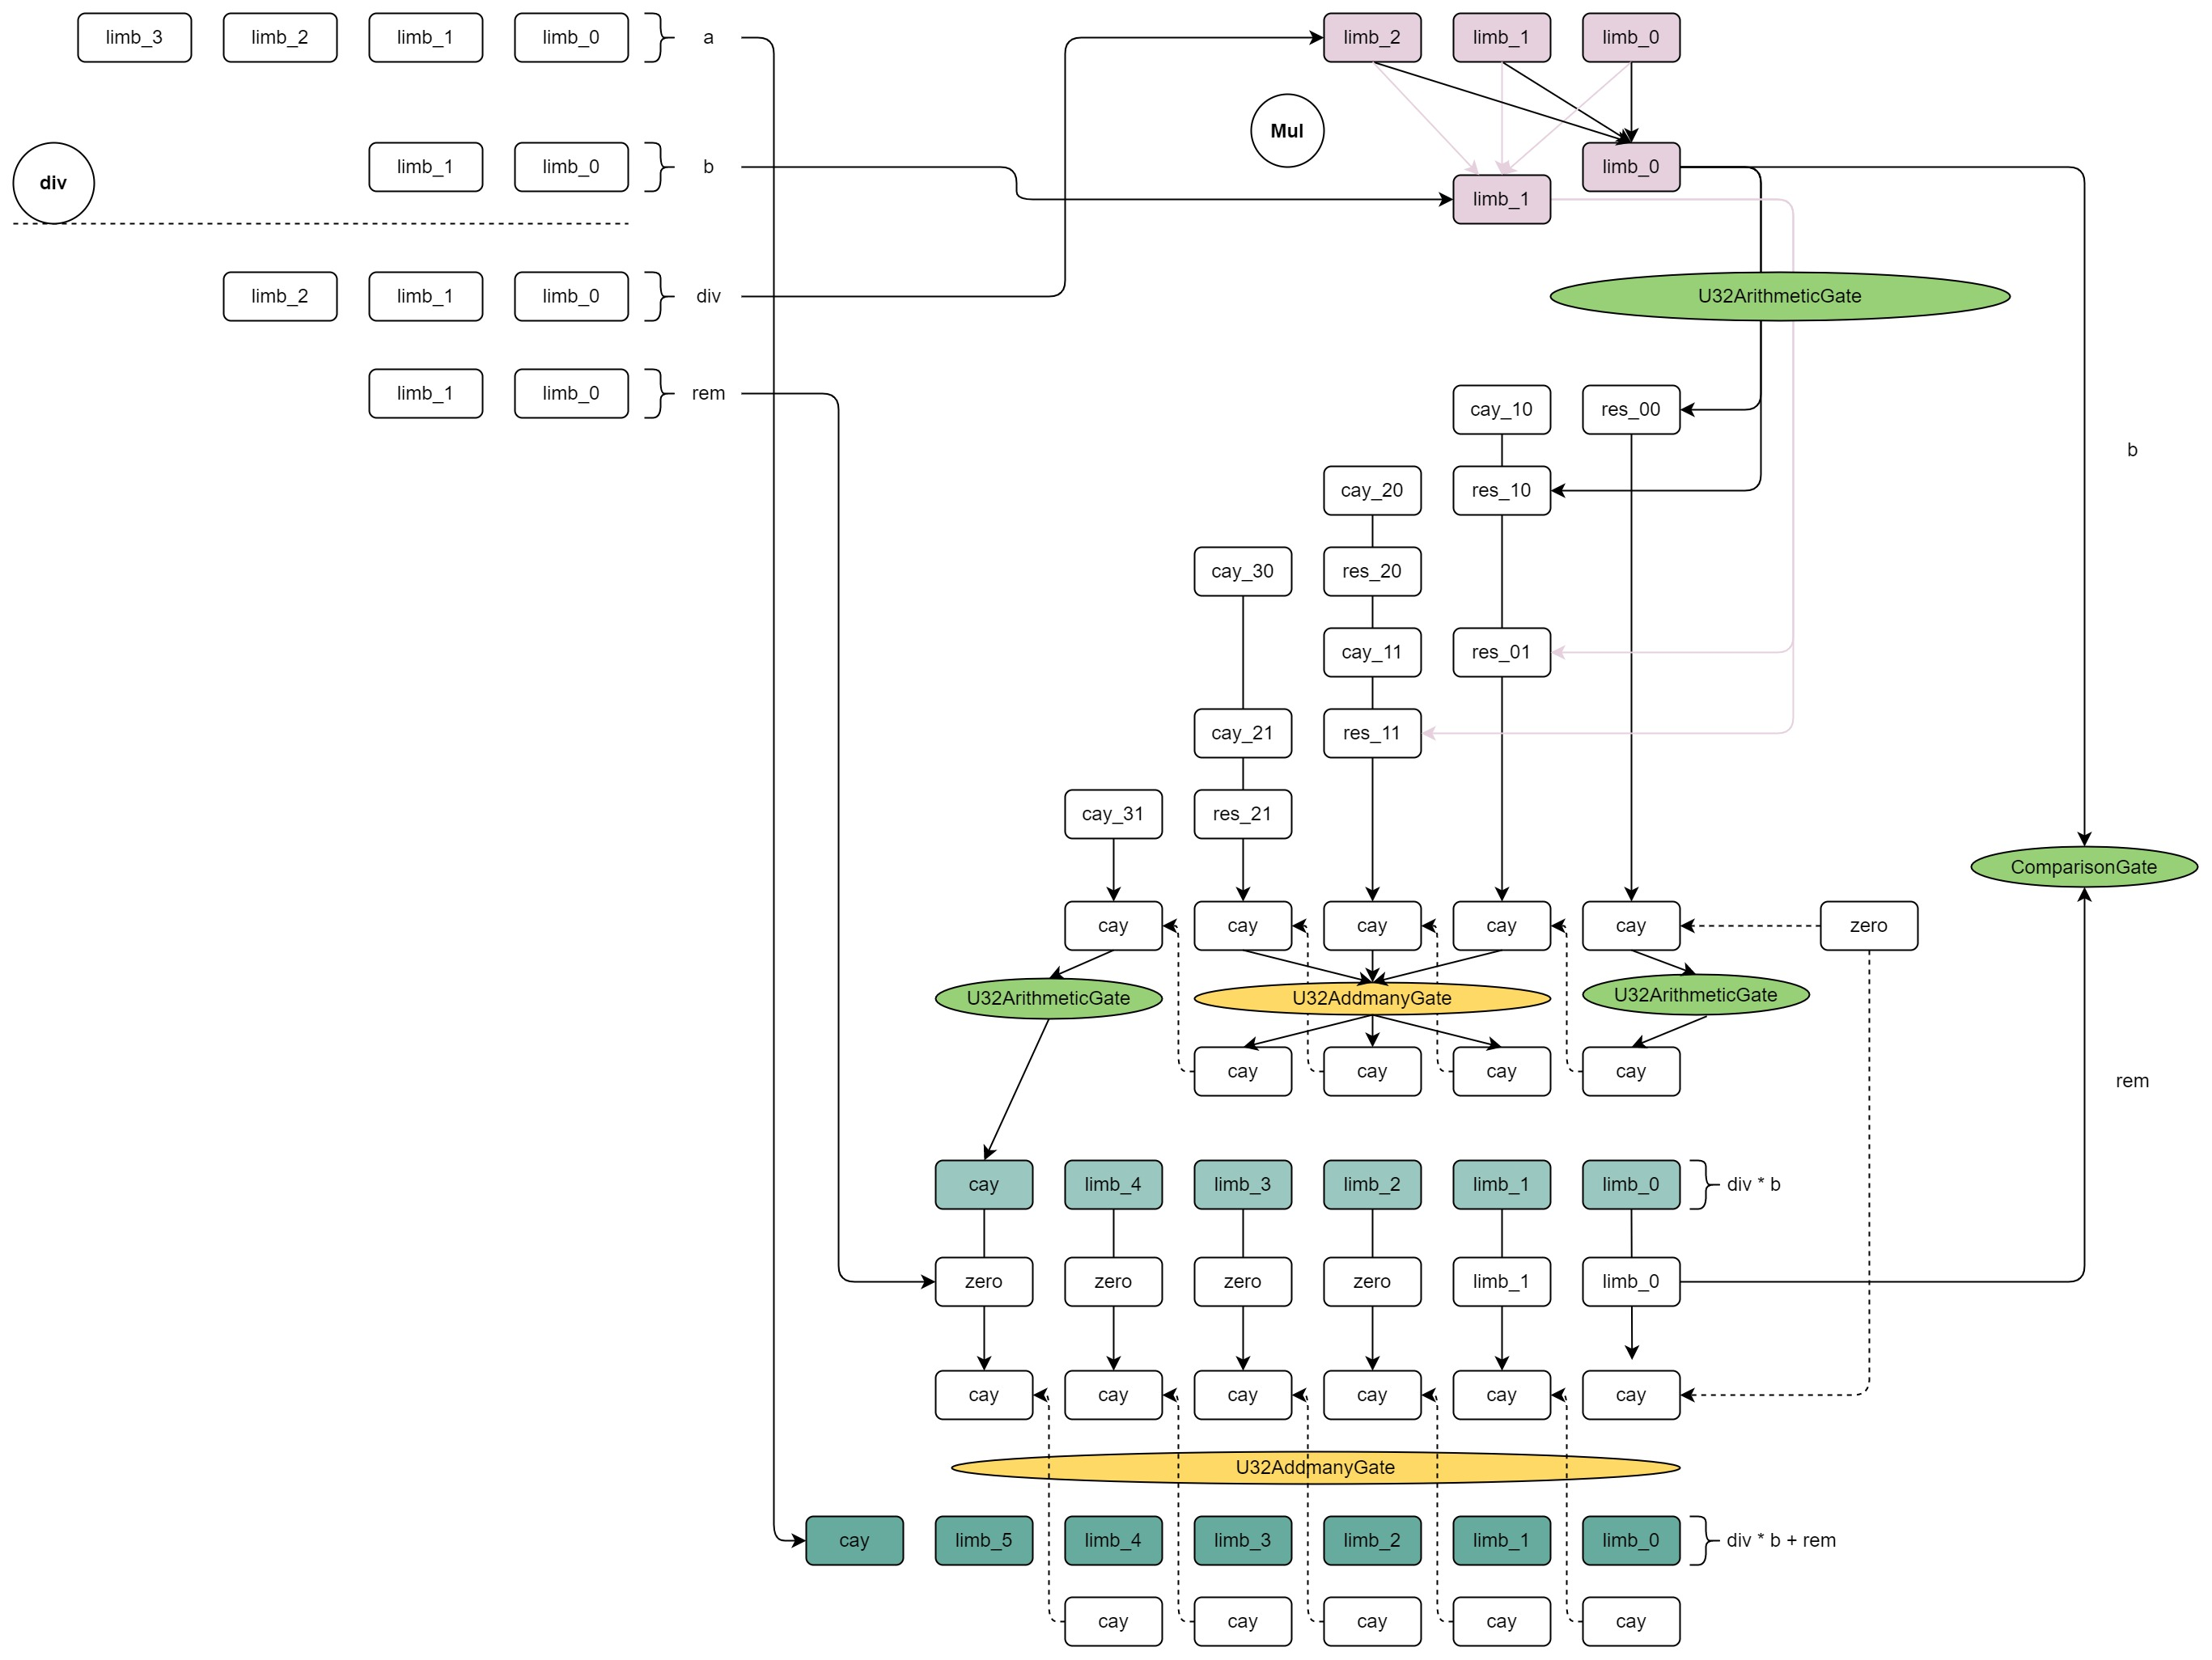
\includegraphics[width=0.8\textwidth]{biguint-div-layout.jpg}
            \caption{biguint-div layout.jpg}
            \label{fig:biguint-div-layout.jpg}
        \end{figure}
    
    \item constraints-info and costs
        \begin{itemize}
            \item Gate type num: 5(U32ArithmeticGate, U32AddManyGate(num-addends: 3), U32AddManyGate(num-addends: 4), ComparisionGate, ArithmeticGate)
            \item Gate instance num: 3 + 3 + 4 + 3 = 13 
            \item U32ArithmeticGate num: 3
            \item U32AddManyGate num: 3
            \item ComparisionGate num: 4
            \item ArithmeticGate num: 3
            \item copy-constraints: 3 * 8 + 4 + 5 + 4 + 4 * 6 + 7 + 1 + 26 + 5 = 100 
            \item max-degree: 4
        \end{itemize}

\end{enumerate}
    \subsubsection{biguint-cmp}

\Par{Target}
Implement the comparison of two biguints.

\Par{Constraints logic}
\begin{itemize}
    \item Split the input to many limbs, such that: \verb|limbs_num = bits / chunks|;
    \item Execute comparison for low bits limbs;
    \item Ensure that the result is determined by the highest limbs which are not equal.
\end{itemize}

\Par{Process layout}
See \figref{fig:biguint-cmp-layout}.
\begin{figure}[!ht]
    \centering
    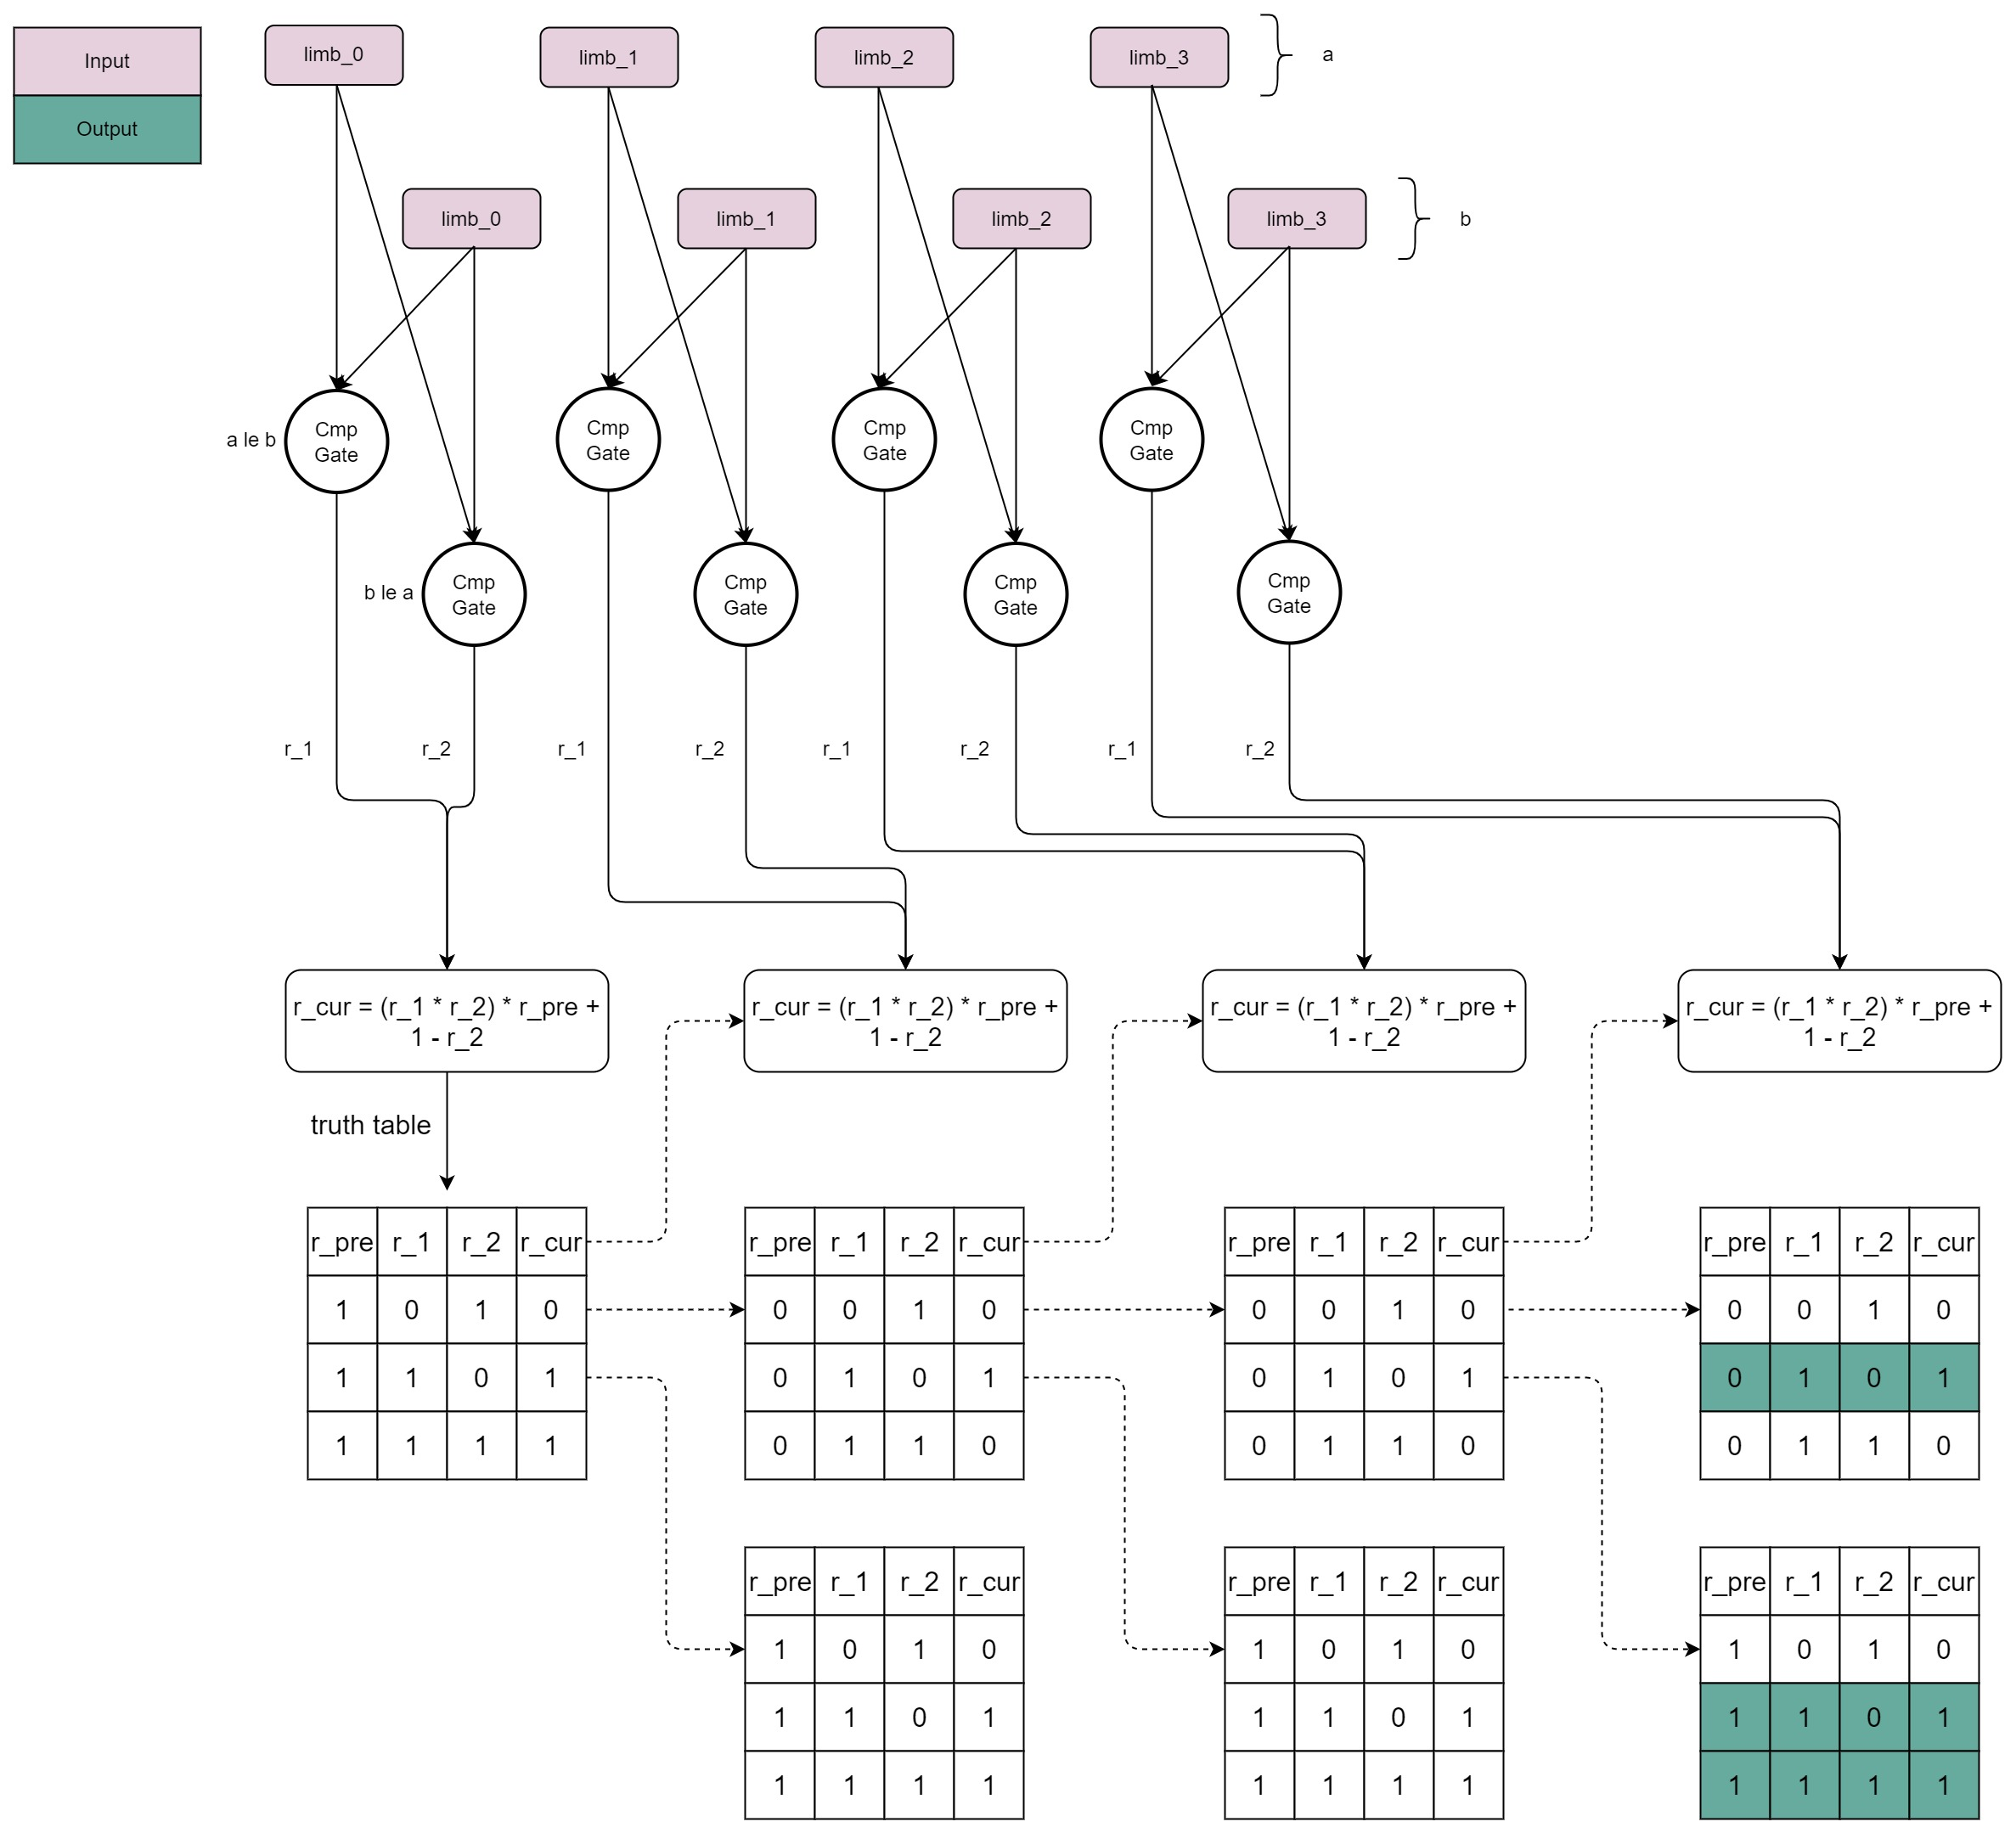
\includegraphics[width=0.8\textwidth]{biguint-cmp-layout.jpg}
    \caption{biguint-cmp layout}
    \label{fig:biguint-cmp-layout}
\end{figure}

\Par{Circuit layout}
See \figref{fig:biguint-cmp-circuit-layout}.
\begin{figure}[!ht]
    \centering
    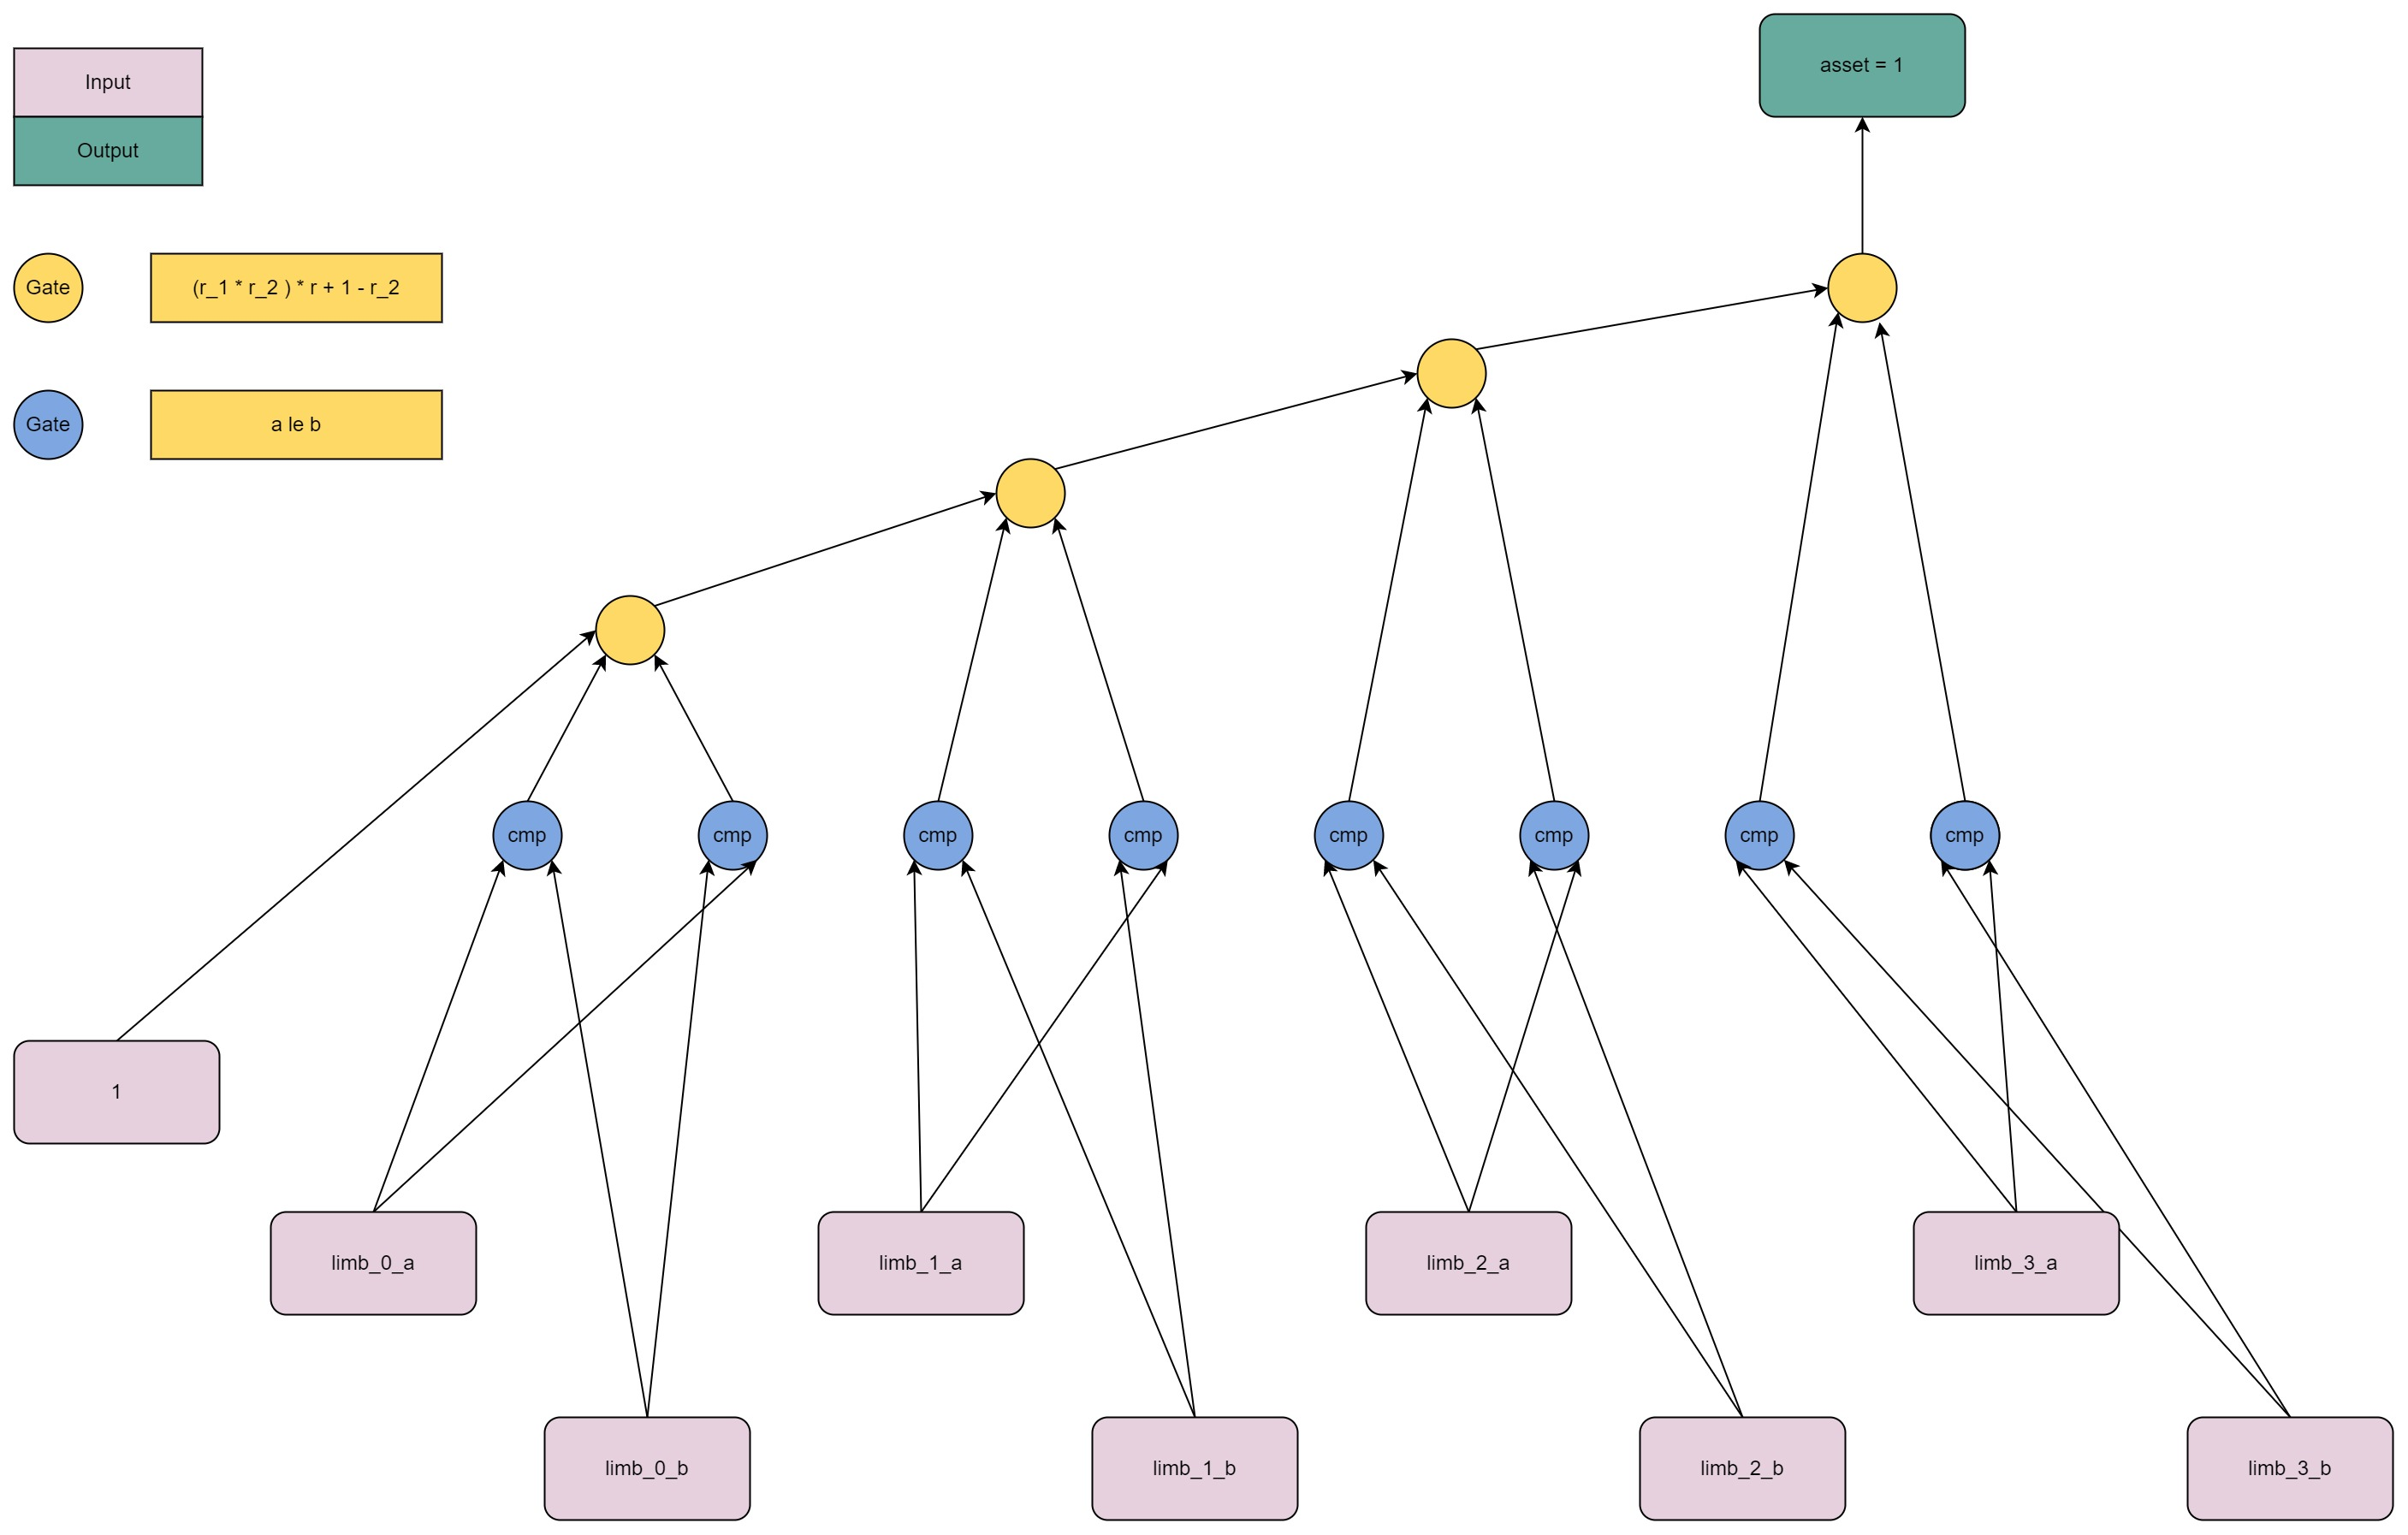
\includegraphics[width=0.8\textwidth]{biguint-cmp-circuit-layout.jpg}
    \caption{biguint-cmp circuit layout}
    \label{fig:biguint-cmp-circuit-layout}
\end{figure}

\Par{Constraints info and costs}
\begin{itemize}
    \item Gate type num: 2 (ComparisionGate, ArithmeticGate)
    \item Gate instance num: $4 \times 2 + 3 = 11$
    \item ComparisionGate num: 8
    \item ArithmeticGate num: 3
    \item copy-constraints: $(4 + 9) \times 4 + 1 = 53$
    \item max-degree: 4
\end{itemize}

    \subsubsection{nonnative-add}
\label{nonnative-add}

\begin{enumerate}
    \item target
        check the additional relation among three nonnative target objects.
    \item constraints-logic
        \begin{itemize}
            \item check equation for gadget,  a + b = c + modular * overflow
            \item check that "c lt modular"
        \end{itemize}
    \item nonnative-add process layout
        \begin{figure}[!ht]
            \centering
            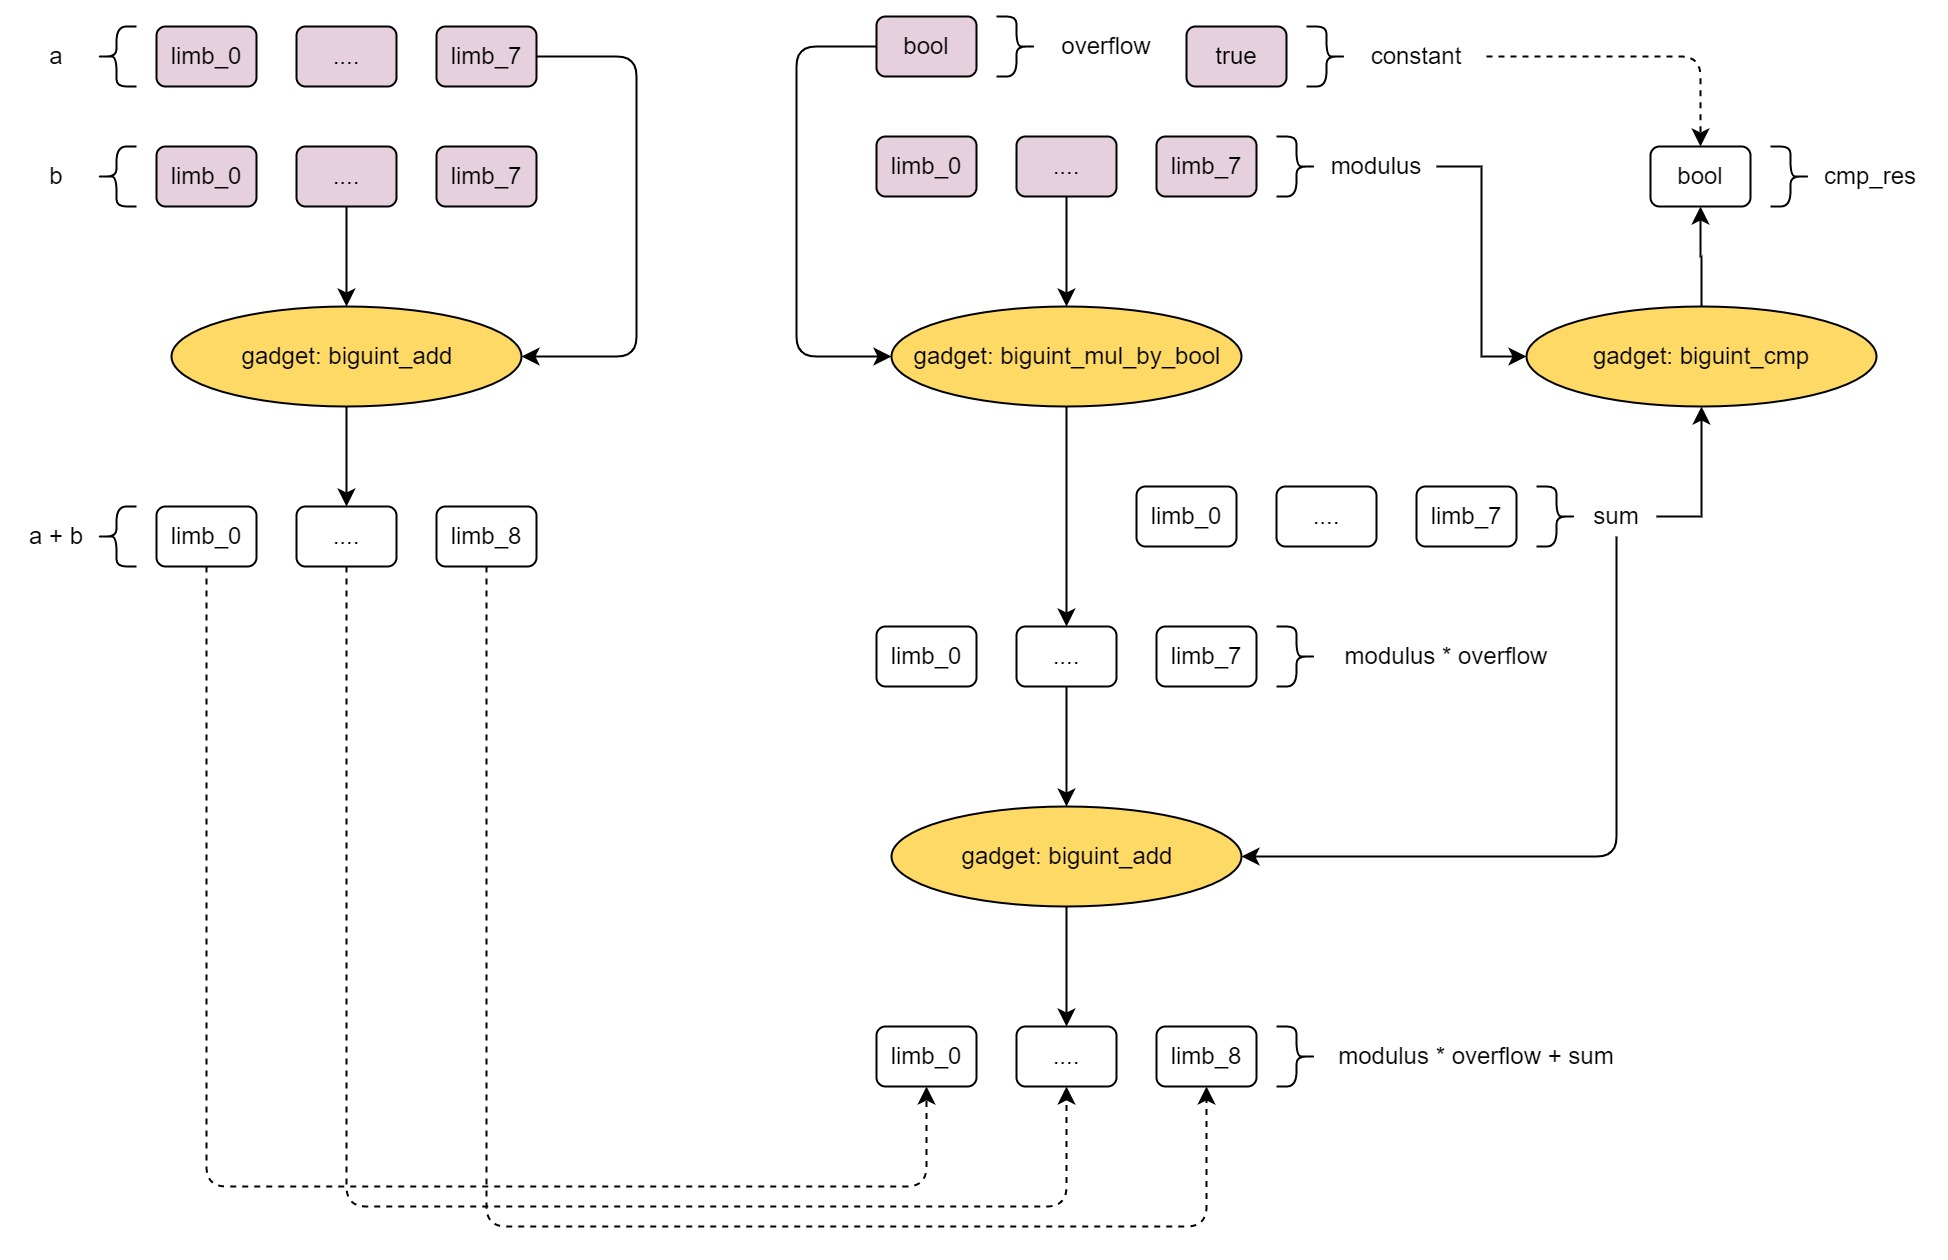
\includegraphics[width=0.8\textwidth]{nonnative-add-layout.jpg}
            \caption{nonnative-add layout}
            \label{fig:nonnative-add-layout}
        \end{figure}
    
    \item constraints-info and costs
        \begin{itemize}
            \item gadget biguint-add num: 2
            \item gadget biguint-mul-by-bool num: 1
            \item gadget biguint-cmp num: 1
            \item gate type num: 3(U32AddManyGate, ComparisonGate, ArithmeticGate)
            \item gate instance num: 23 = 3(U32AddManyGate) + 16(ComparisonGate) + 2(ArithmeticGate(1,0)) + 1(ArithmeticGate(1,-1)) + 1(ArithmeticGate(1,1))
            \item copy-constraints: 186 = 32 * 2{biguint-add} + 9{biguint-mul-by-bool} + 9 + (4 + 9) * 8{biguint-cmp} = 186
        \end{itemize}

    \item questions
        \begin{itemize}
            \item when set value to sum?
        \end{itemize}

\end{enumerate}
    \subsubsection{nonnative-sub}
\label{nonnative-sub}

\begin{enumerate}
    \item target
        check the substract relation among three nonnative target objects.
    \item constraints-logic
        \begin{itemize}
            \item check equation for gadget,  diff + b = a + modular * overflow
            \item check that "overflow is bool"
            \item check that "diff.limbs is range U32"
        \end{itemize}
    \item nonnative-sub process layout
        \begin{figure}[!ht]
            \centering
            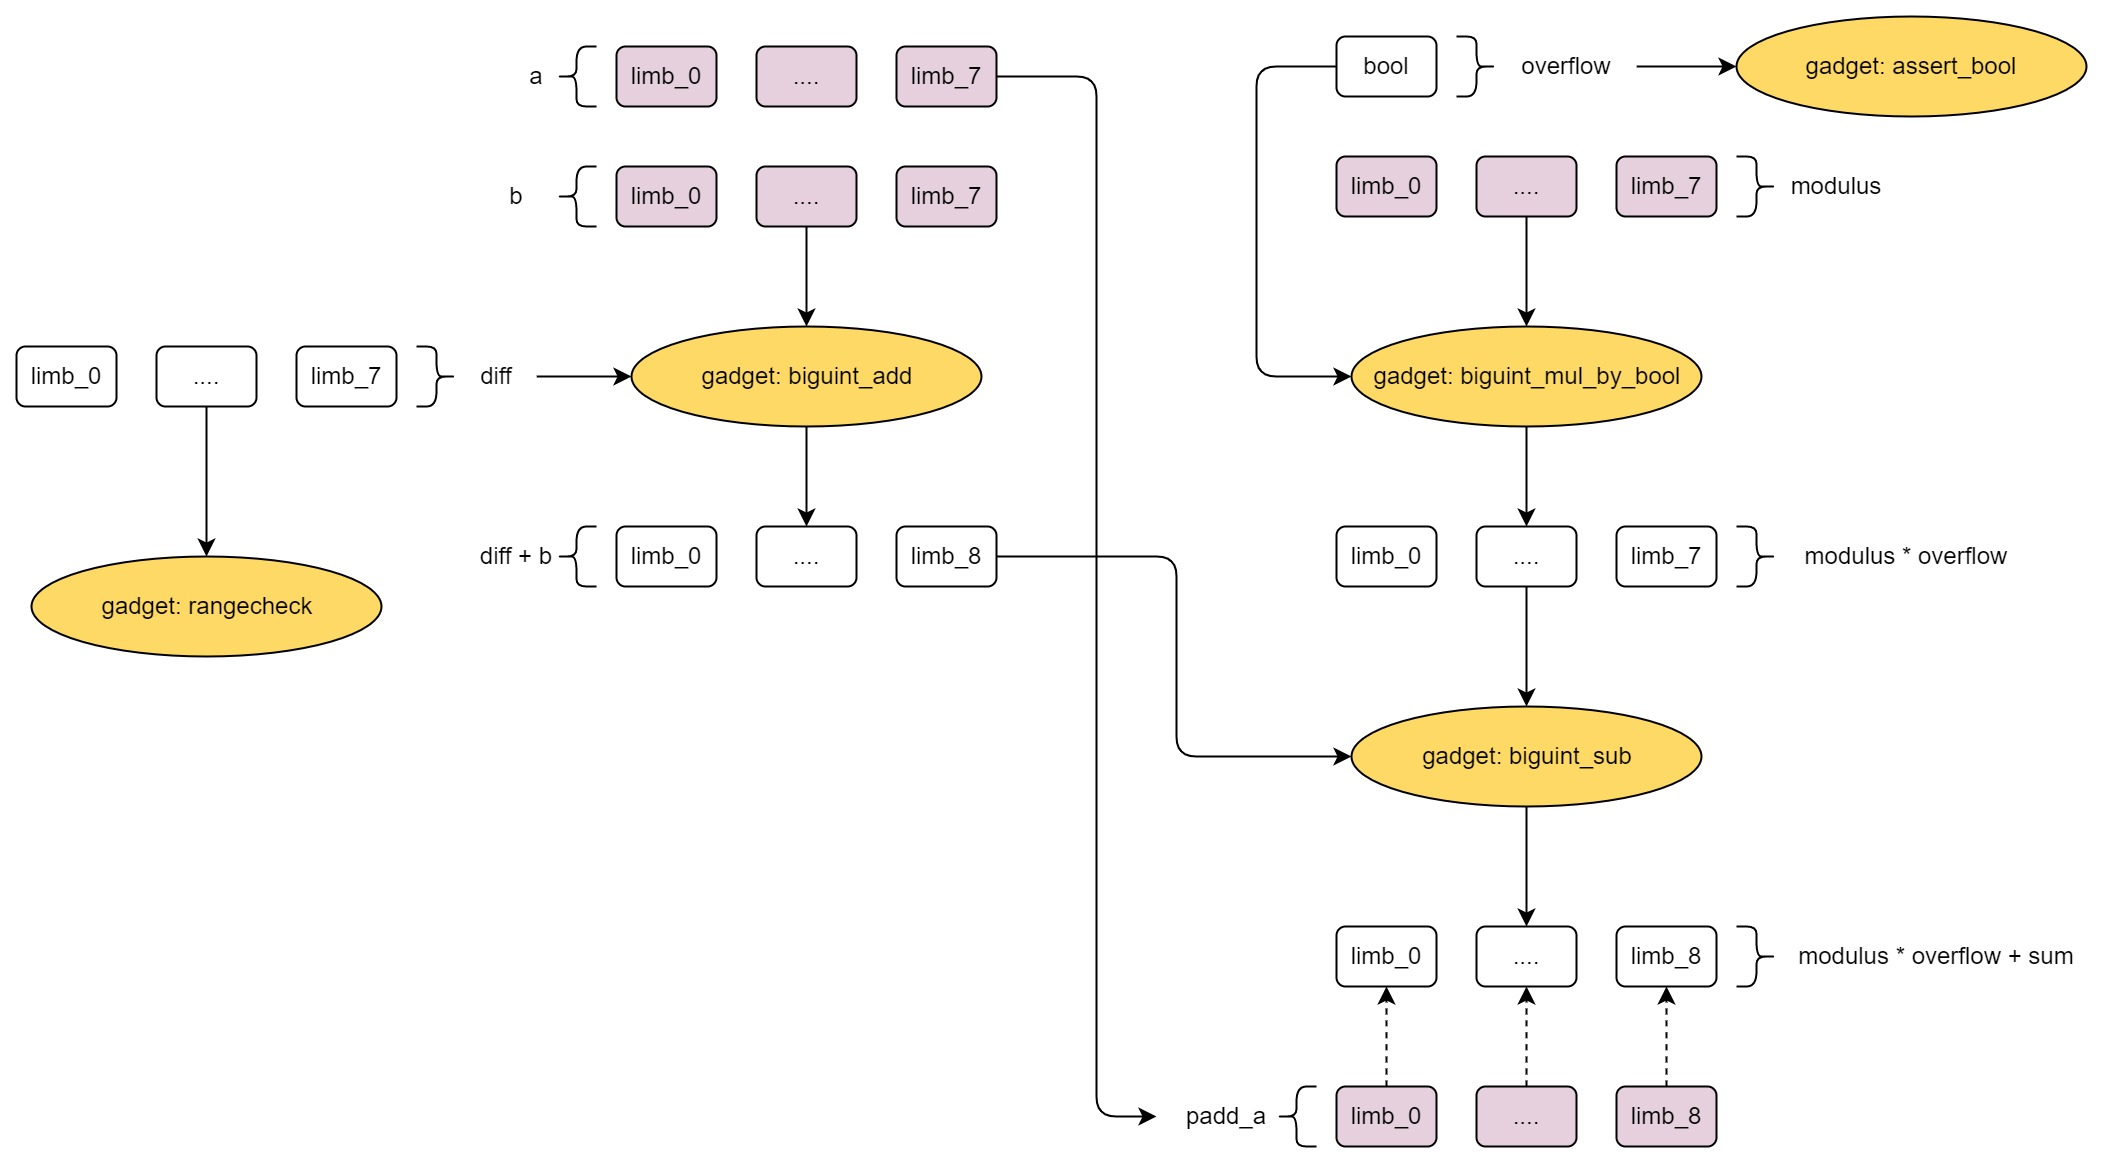
\includegraphics[width=0.8\textwidth]{nonnative-sub-layout.jpg}
            \caption{nonnative-sub layout}
            \label{fig:nonnative-sub-layout}
        \end{figure}
    
    \item constraints-info and costs
        \begin{itemize}
            \item gadget biguint-add num: 1
            \item gadget biguint-sub num: 1
            \item gadget biguint-mul-by-bool num: 1
            \item gadget u32rangecheck num: 1
            \item gadget assert-bool num: 1
            \item gate type num: 4(U32AddManyGate, U32SubtractionGate, U32RangeCheckGate, ArithmeticGate)
            \item gate instance num: 7 = 2(U32AddManyGate) + 2(U32SubtractionGate) + 1(U32RangeCheckGate) + 1(ArithmeticGate(1,0)) + 1(ArithmeticGate(1,-1))
            \item copy-constraints: 89 = 32{biguint-add num} + 27{U32SubtractionGate} + 9{biguint-mul-by-bool} + 8{u32rangecheck} + 4{assert-bool} + 9
        \end{itemize}

    \item questions
        \begin{itemize}
            \item why not constraint for overflow at nonnative-add?
            \item why not make u32rangecheck for input at nonnative-add?
        \end{itemize}

\end{enumerate}
    \subsubsection{nonnative-mul}
\label{nonnative-mul}

\begin{enumerate}
    \item target
        check the multiplicatipn relation among three nonnative target objects.
    \item constraints-logic
        \begin{itemize}
            \item check equation for gadget,  a * b = prod + modular * overflow
            \item check that "overflow.limb is U32"
            \item check that "prod.limb is U32"
        \end{itemize}
    \item nonnative-mul process layout
        \begin{figure}[!ht]
            \centering
            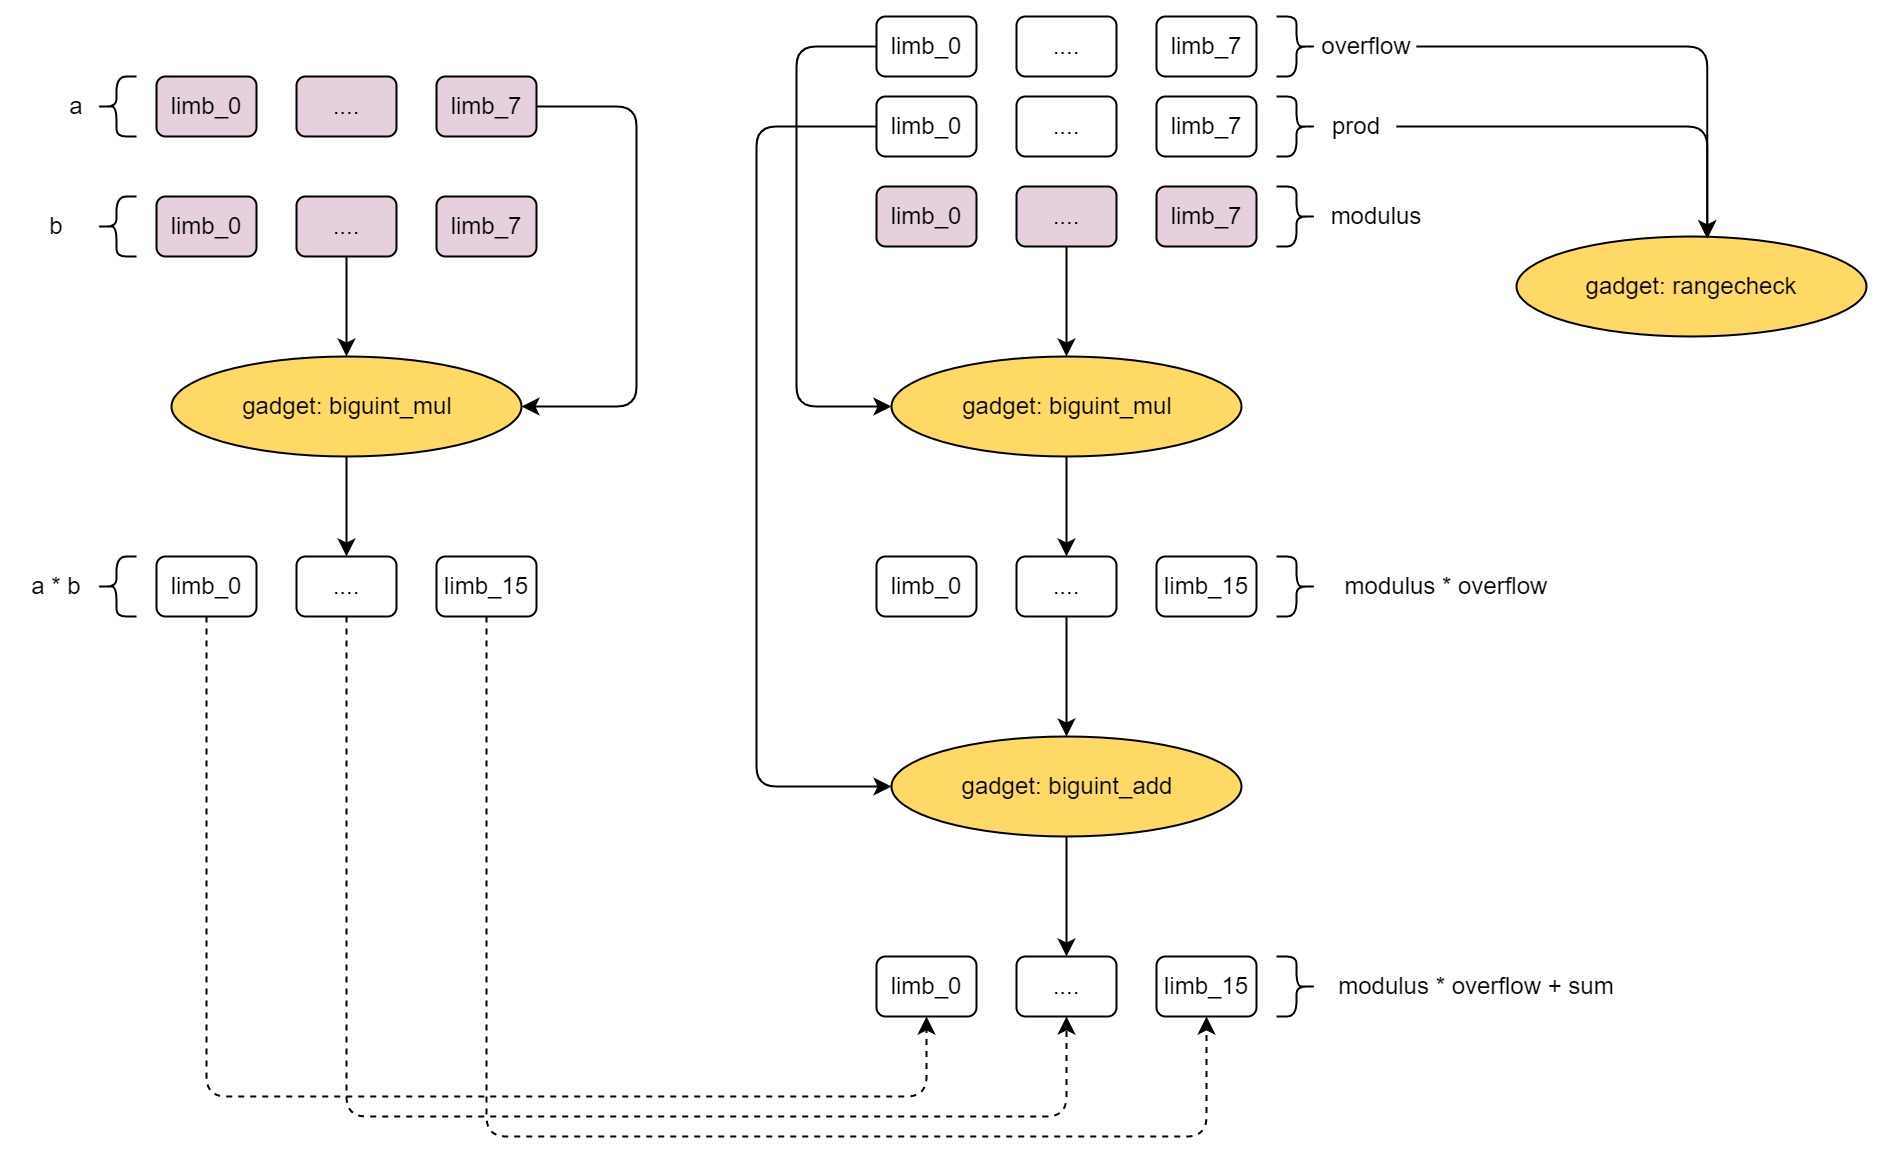
\includegraphics[width=0.8\textwidth]{nonnative-mul-layout.jpg}
            \caption{nonnative-mul layout}
            \label{fig:nonnative-mul-layout}
        \end{figure}
    
    \item constraints-info and costs
        \begin{itemize}
            \item gadget biguint-add num: 1
            \item gadget biguint-mul num: 2
            \item gadget u32rangecheck num: 2
            \item gate type num: 9 = 7(U32AddManyGate{3,5,7,9,11,13,15}) + 1(U32RangeCheckGate) + 1(U32ArithmeticGate)
            \item gate instance num: 37 = 2(u32rangecheck) + 8(biguint-mul: constant-input) + 22(biguint-mul) + 1 + 3(biguint-add)
            \item copy-constraints: 583 = 8 * 2(u32rangecheck) + 3 * 3 + (4 + 6 + 8 + 10 + 12 + 14 + 16) * 4 + (8 * 8) * 3 + 17 * 4 + 18
        \end{itemize}

\end{enumerate}
    \subsubsection{nonnative-inv}

\Par{Target}
Check the modular inverse relation among three nonnative target objects.

\Par{Constraints logic}
\begin{itemize}
    \item Check equation for gadget: \verb|a * inv_a = 1 + modular * div|.
\end{itemize}

\Par{Process layout}
See \figref{fig:nonnative-inv-layout}.
\begin{figure}[!ht]
    \centering
    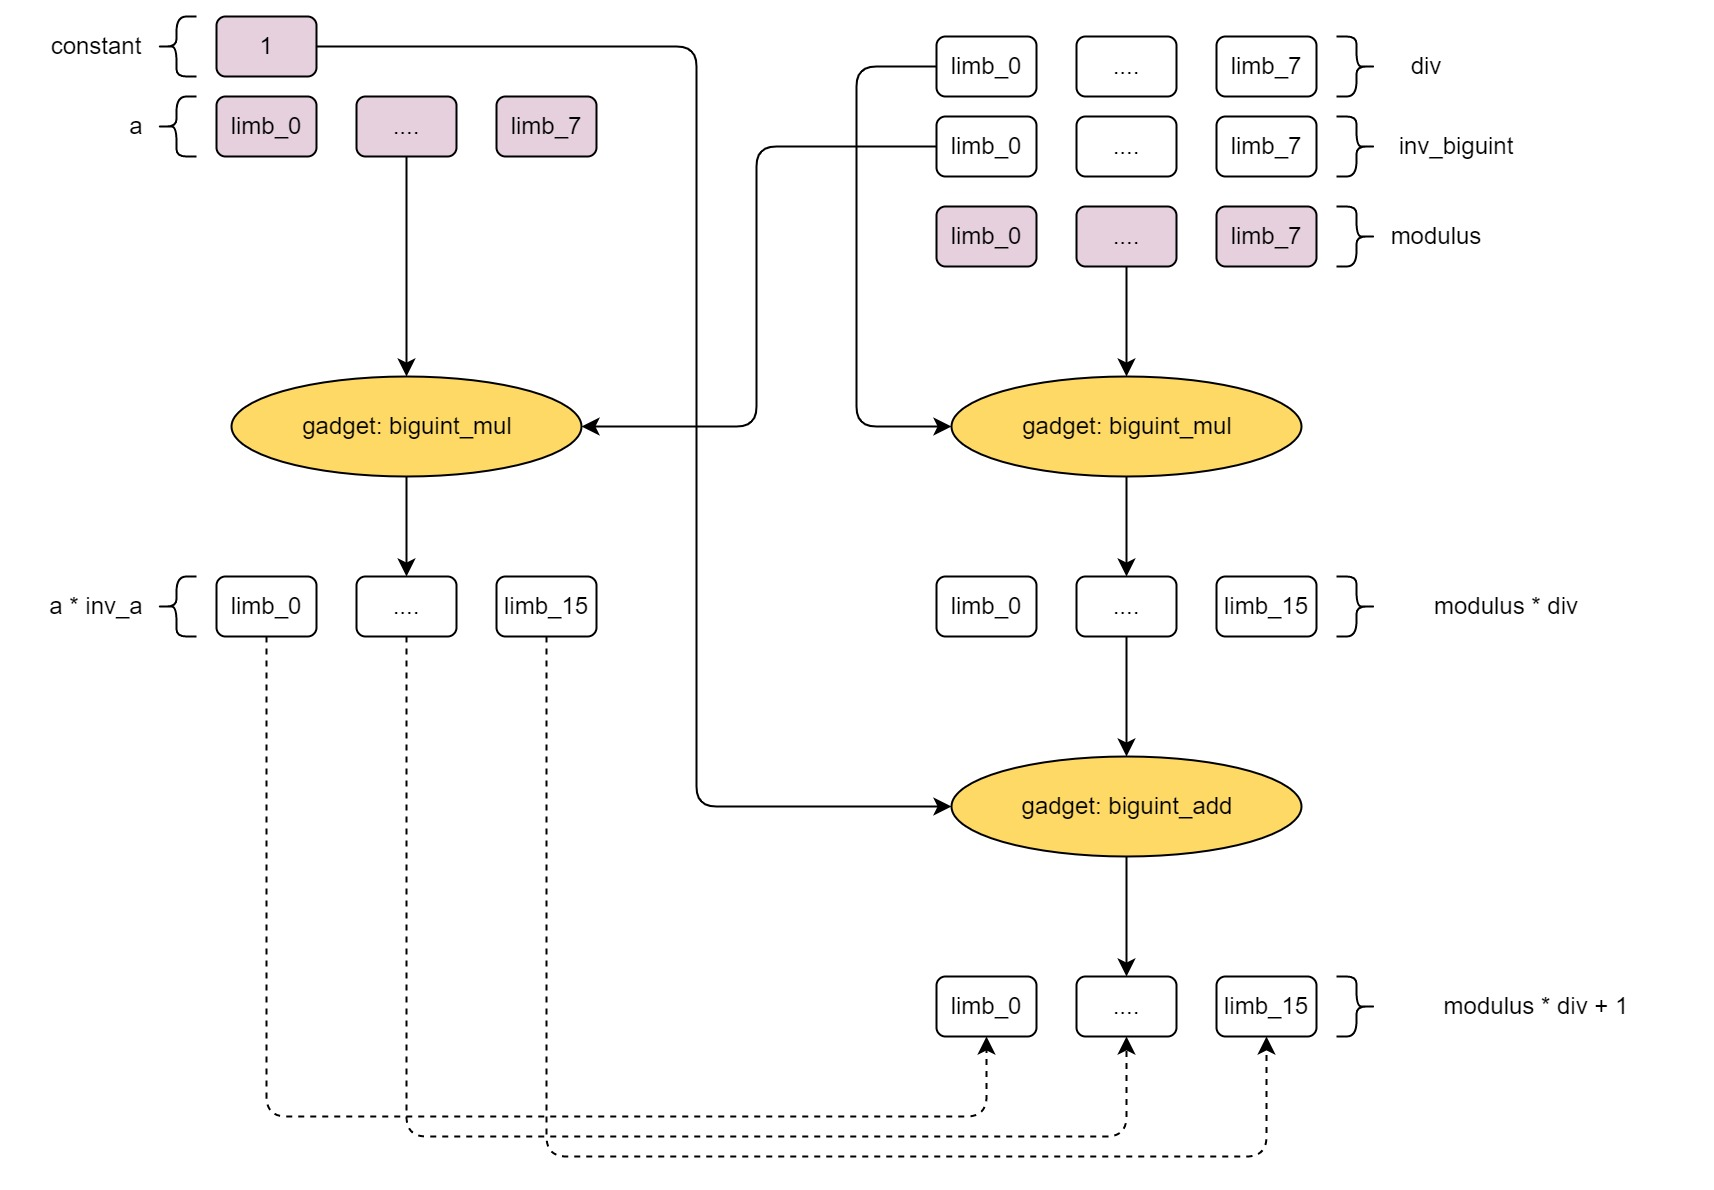
\includegraphics[width=0.8\textwidth]{nonnative-inv-layout.jpg}
    \caption{nonnative-inv layout}
    \label{fig:nonnative-inv-layout}
\end{figure}

\Par{Constraints info and costs}
\begin{itemize}
    \item gadget biguint-add num: 1
    \item gadget biguint-mul num: 2
    \item gate type num: 8 = 7(U32AddManyGate\{3,5,7,9,11,13,15\}) + 1(U32ArithmeticGate)
    \item gate instance num: 56 = (8 * 8 + 2) * 2 / 3 + 5(U32AddManyGate{3}) + 5 + 2(U32AddManyGate{15})
    \item copy-constraints: 762 = (8 * 8 + 2) * 2 * 3 + 21 * 4 + (6 + 8 + 10 + 12 + 14) * 4 + 4 * 16 + 18
\end{itemize}

    \section{curve-add}
\label{curve-add}

Take curve-secp256k1 as example, the same as other texs.

\begin{enumerate}
    \item target
        implement the addition of two different curve points. this is a incomplete addition, you can refer to The halo2 Book \cite{website:halo2-book} to learn more about it.
    \item constraints-logic
        \begin{figure}[!ht]
            \centering
            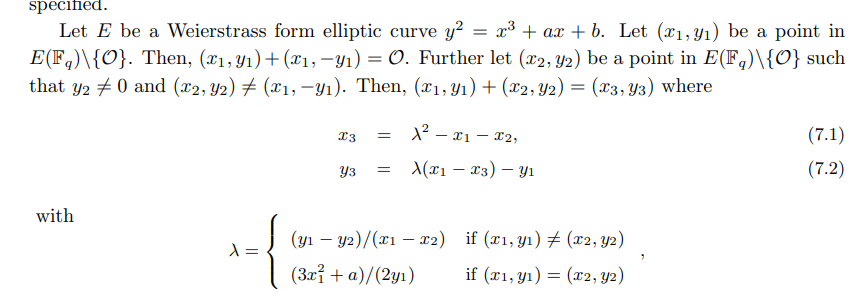
\includegraphics[width=0.8\textwidth]{curve-add.jpg}
            \caption{curve-add}
            \label{fig:curve-add}
        \end{figure}
    \item curve-add process layout
        \begin{figure}[!ht]
            \centering
            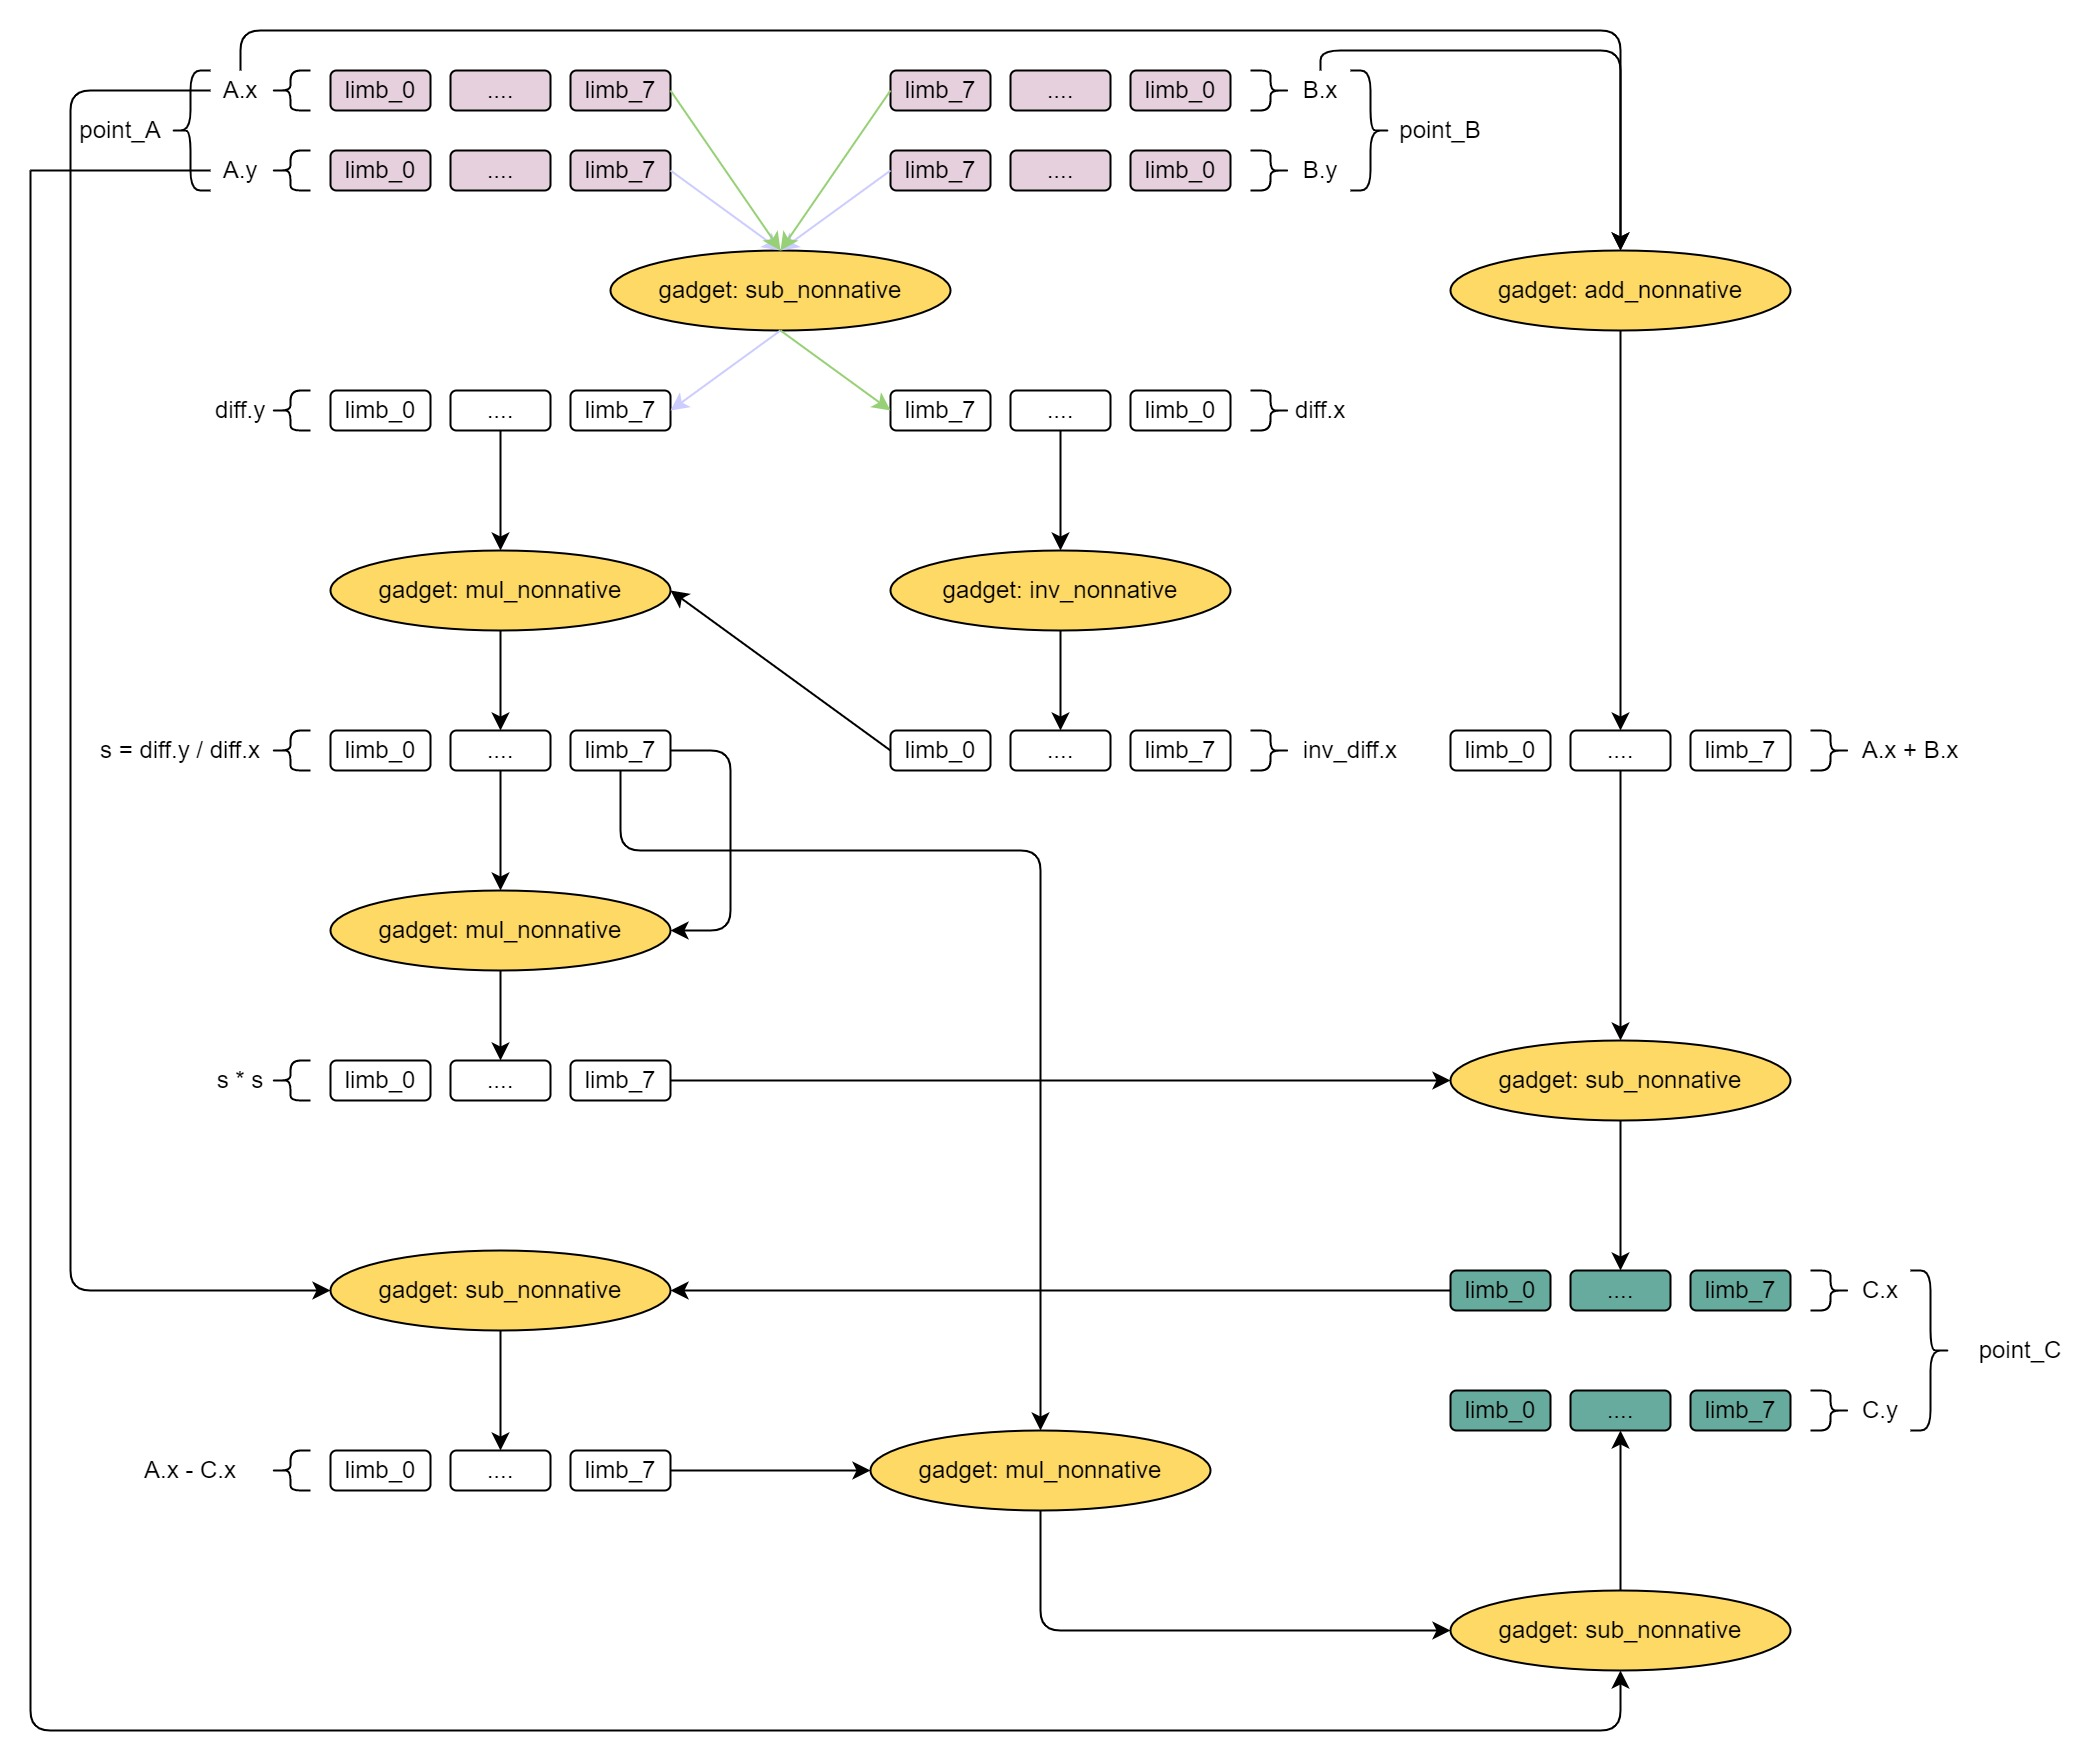
\includegraphics[width=0.8\textwidth]{curve-add-layout.jpg}
            \caption{curve-add layout}
            \label{fig:curve-add-layout}
        \end{figure}
    
    \item constraints-info and costs
        \begin{itemize}
            \item gadget-sub-nonnative num: 5
            \item gadget-add-nonnative num: 1
            \item gadget-mul-nonnative num: 3
            \item gadget-inv-nonnative num: 1
            \item gate type num: 
            \item gate instance num: 
        \end{itemize}

\end{enumerate}
    %\printbibliography[heading=bibintoc, title=\ebibname]%
\end{document}

    \subsubsection{biguint-add}

\Par{Target}
Implement the addition of two biguints.

\Par{Constraints logic}
\begin{itemize}
    \item Equation for gates;
    \item Sumcheck between output and limbs;
    \item Rangecheck for limbs.
\end{itemize}

\Par{Circuit layout}
See \figref{fig:biguint-add-circuit-layout}.
\begin{figure}[!ht]
    \centering
    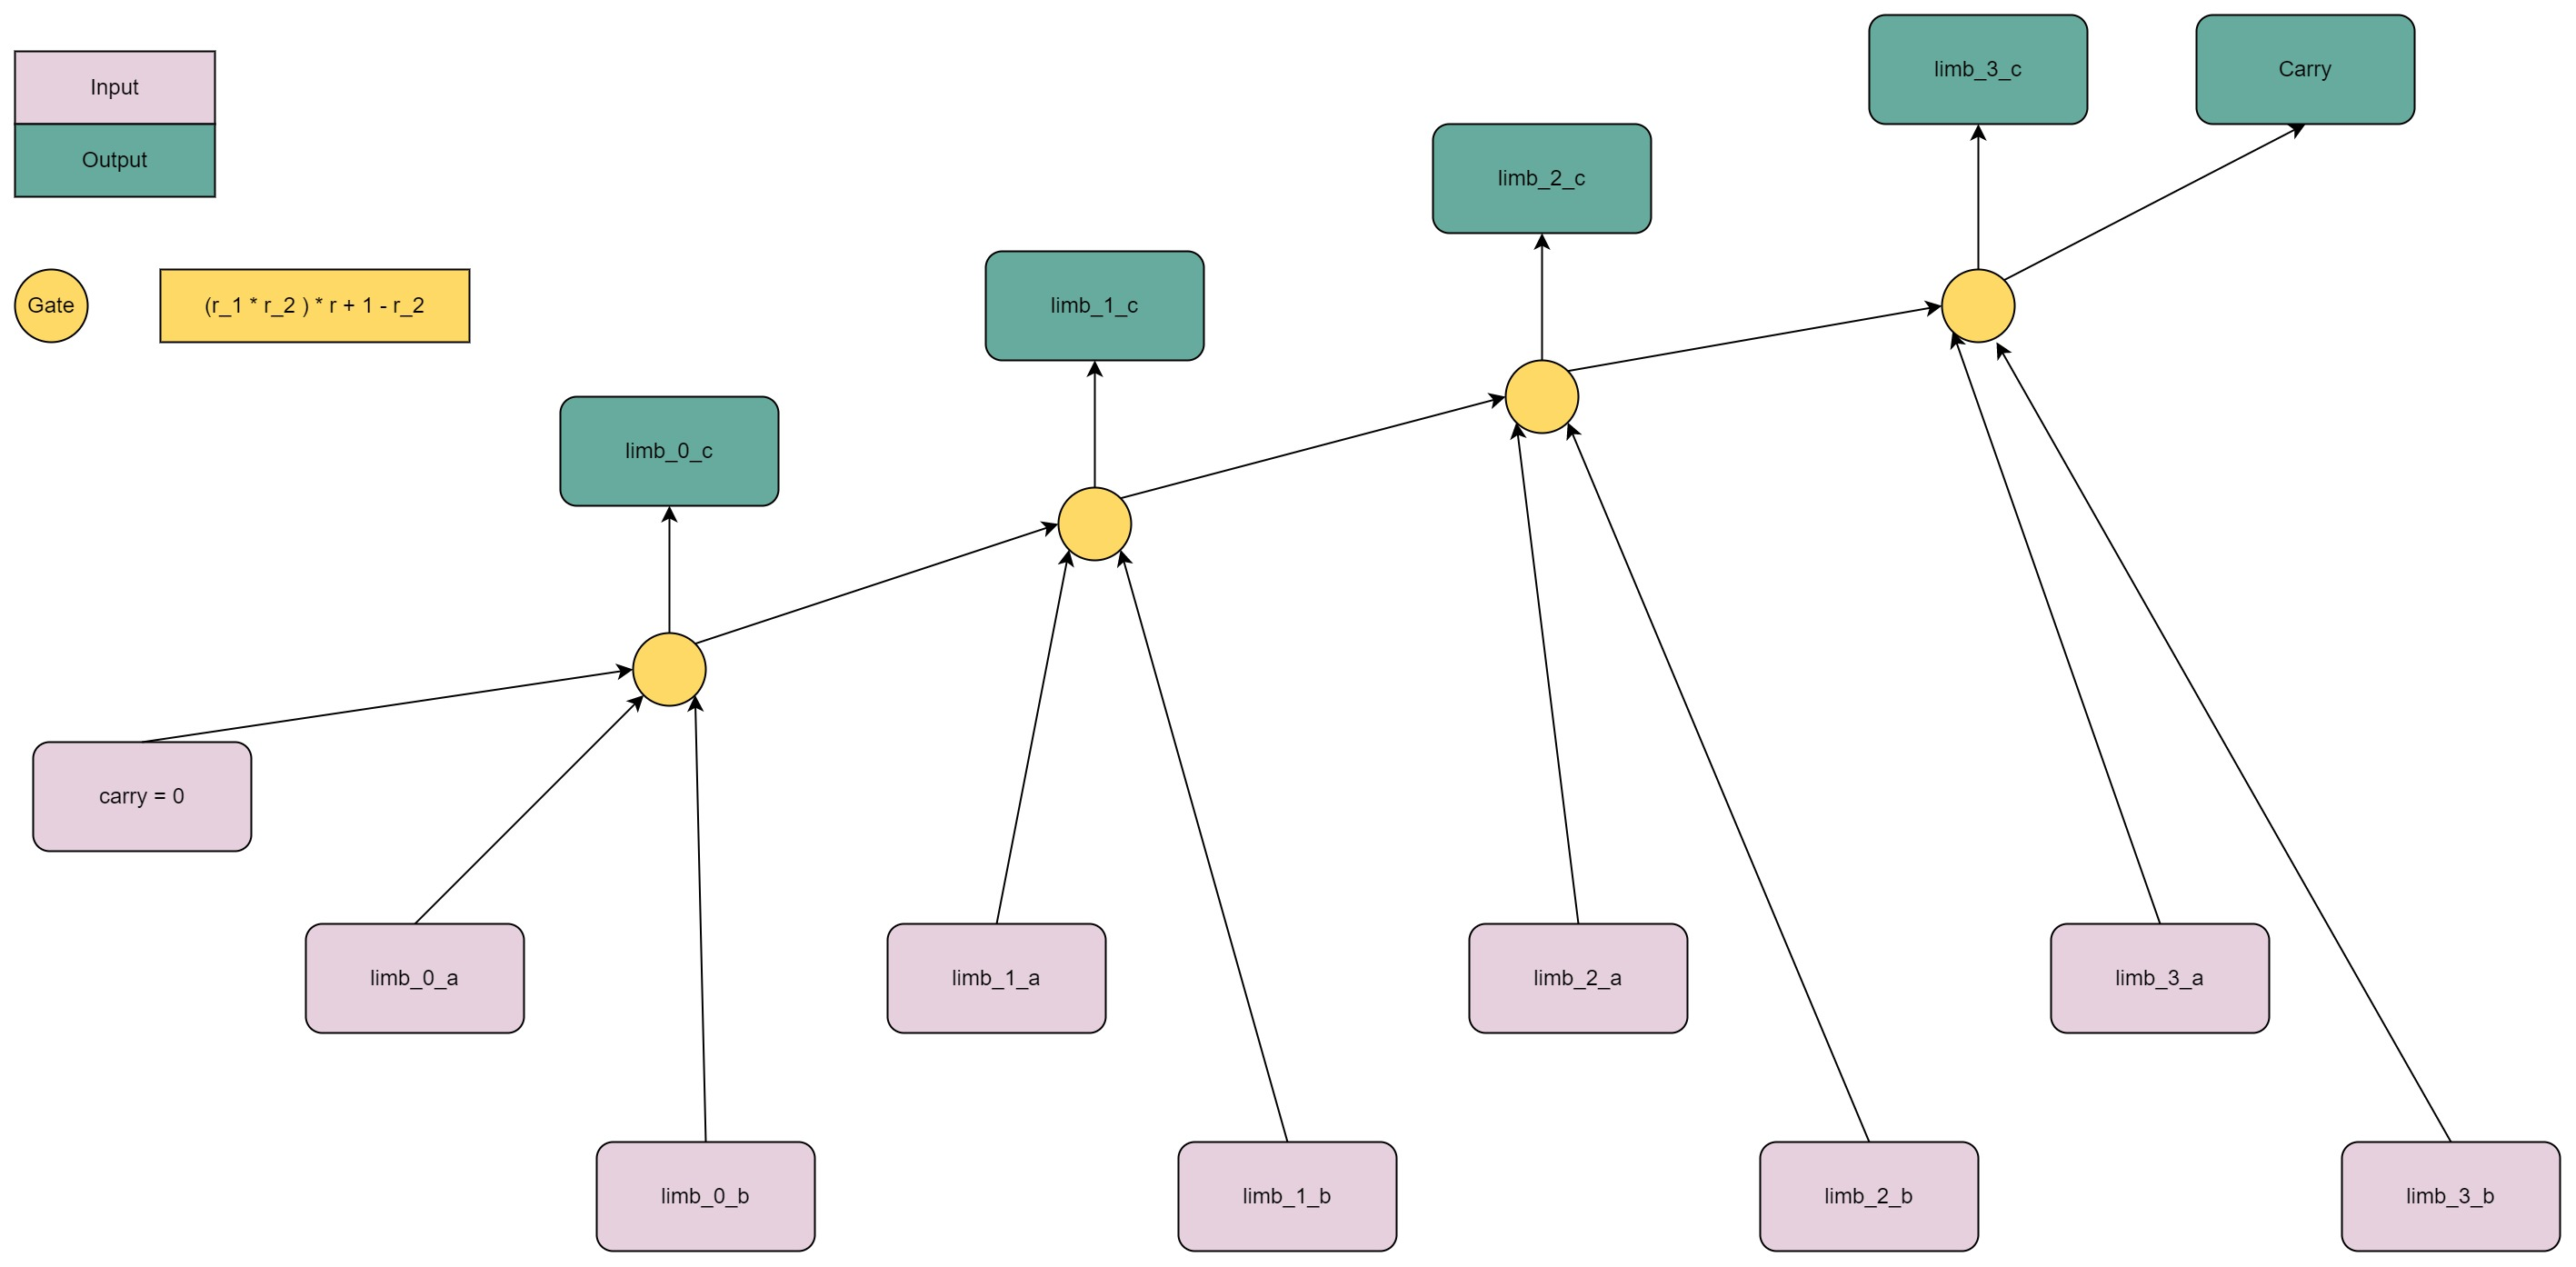
\includegraphics[width=0.8\textwidth]{biguint-add-circuit-layout.jpg}
    \caption{biguint-add circuit layout}
    \label{fig:biguint-add-circuit-layout}
\end{figure}

\Par{Trace layout}
See \figref{fig:biguint-add-trace-layout}.
\begin{figure}[!ht]
    \centering
    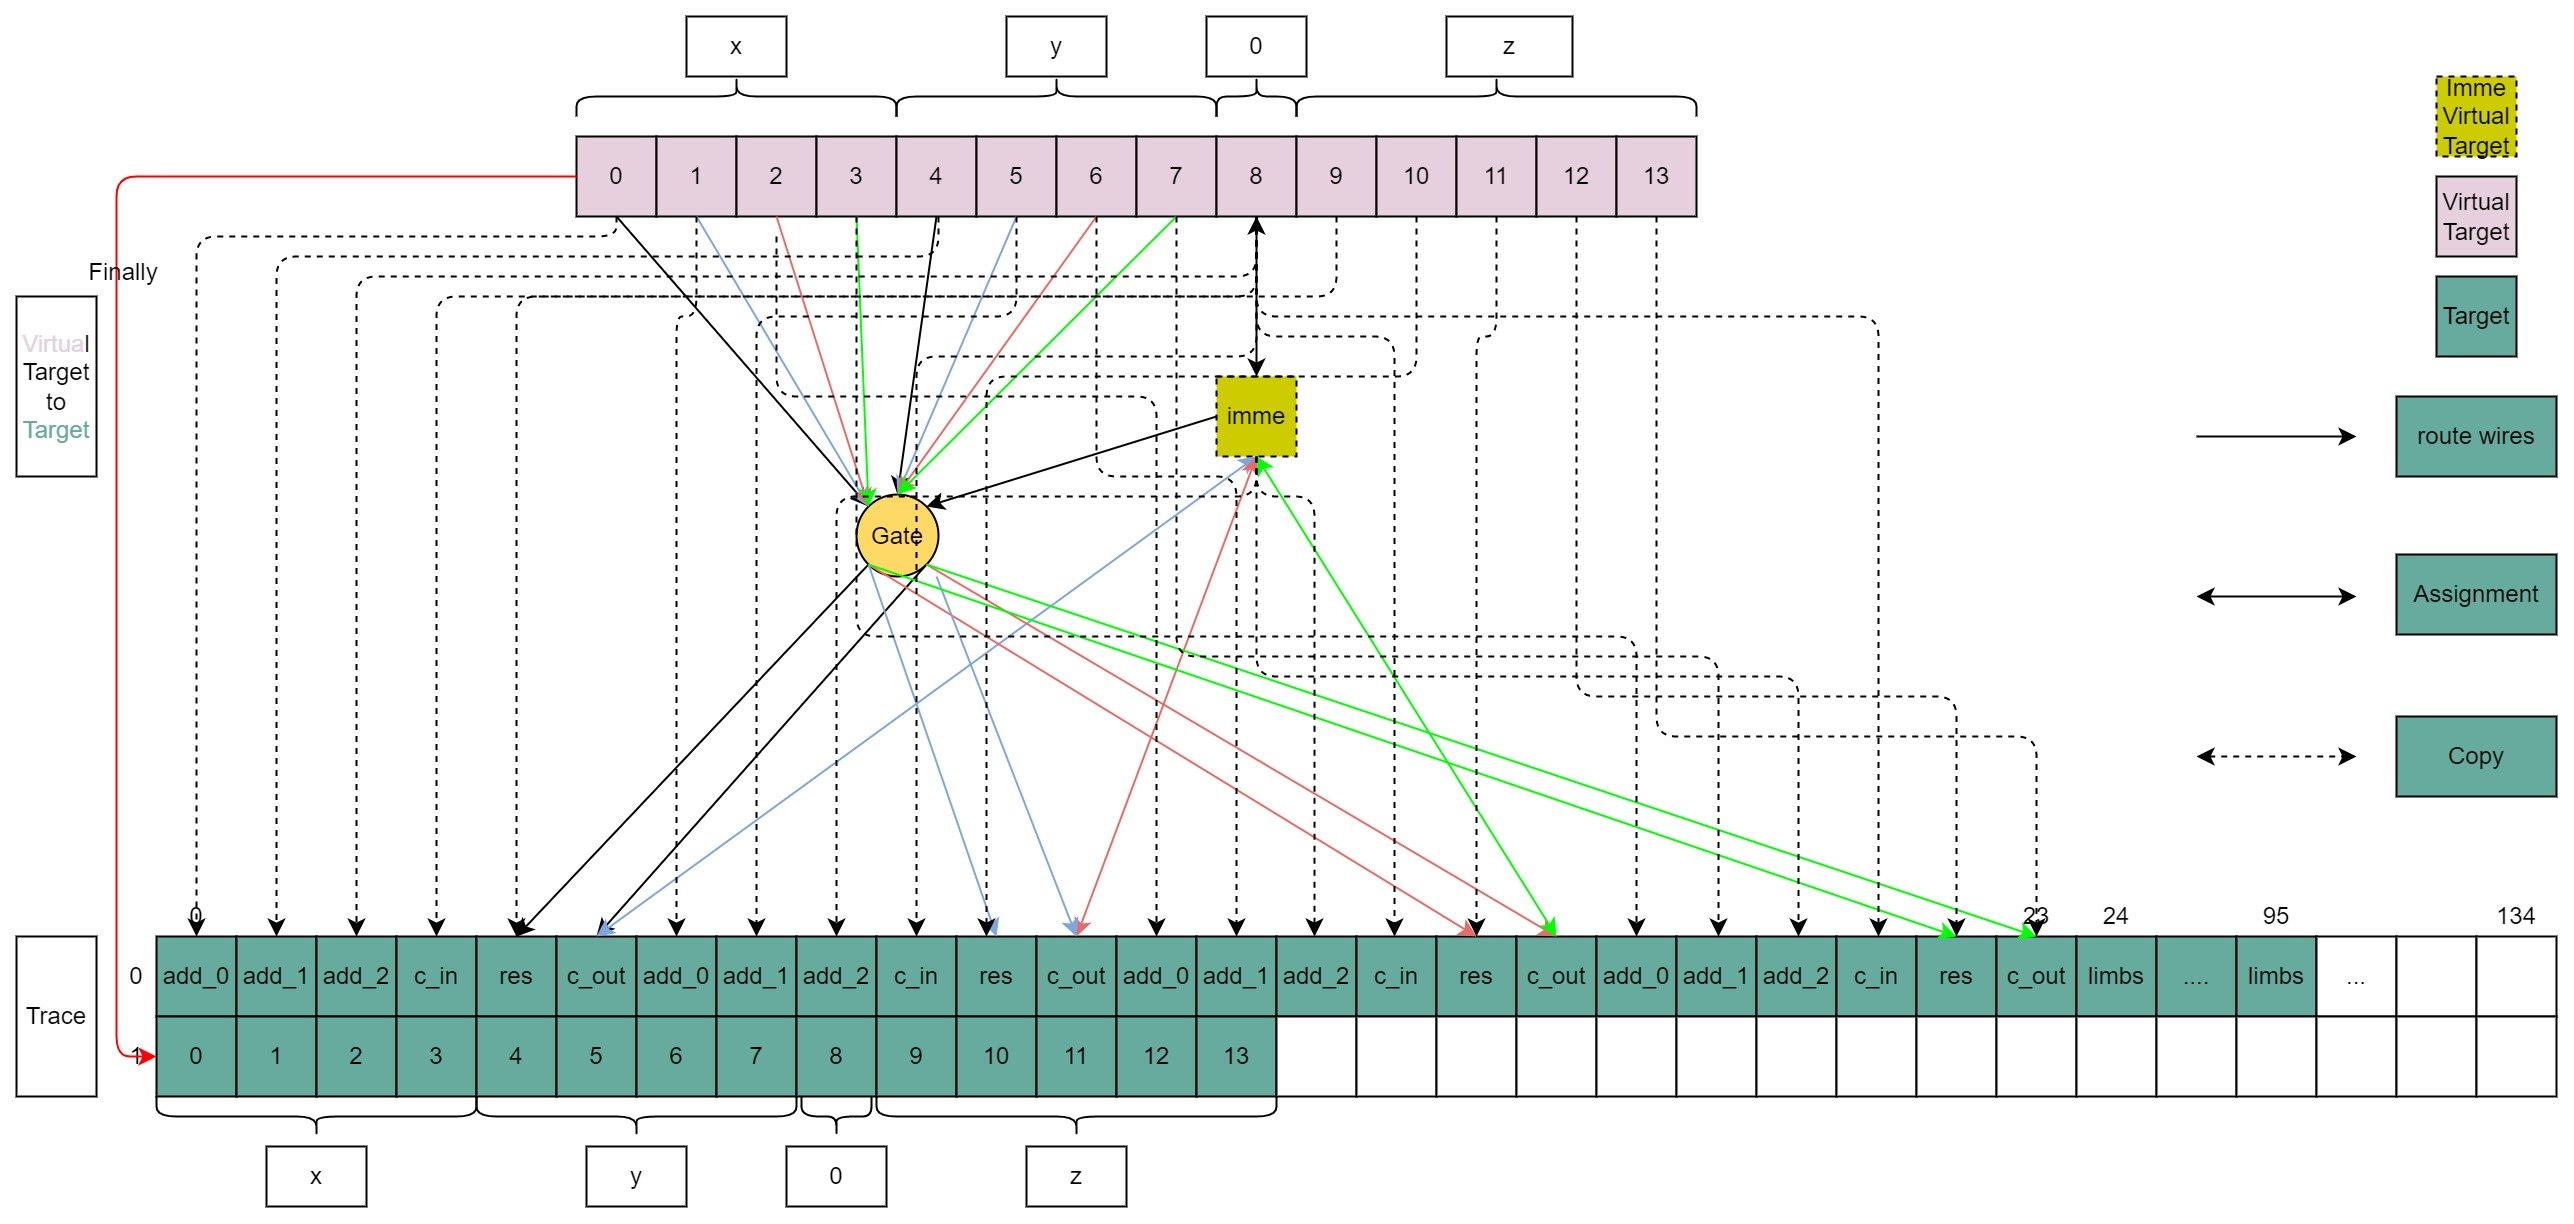
\includegraphics[width=0.8\textwidth]{biguint-add-trace-layout.jpg}
    \caption{biguint-add trace layout}
    \label{fig:biguint-add-trace-layout}
\end{figure}

\Par{Constraints info and costs}
\begin{itemize}
    \item gate type num: 1 (U32AddManyGate)
    \item gate ops num: limbs-num
    \item gate instance num: ceil(limbs-num / gate.ops)
    \item copy-constraints: limbs-num * 4
    \item max-degree: 4 (\verb|1 << limb-bits|)
\end{itemize}

\Par{Questions}
\begin{itemize}
    \item Why not make rangecheck constraint for inputs?
    \item Why not make copy constraint between cur-c-in and last-c-out?
\end{itemize}

    \subsubsection{biguint-sub}

\Par{Target}
Implement the substraction of two biguints.

\Par{Constraints logic}
\begin{itemize}
    \item Equation for gate;
    \item Sumcheck for ouptput;
    \item Rangecheck for limbs.
\end{itemize}

\Par{Circuit layout}
See \figref{fig:biguint-sub-circuit-layout}.
\begin{figure}[!ht]
    \centering
    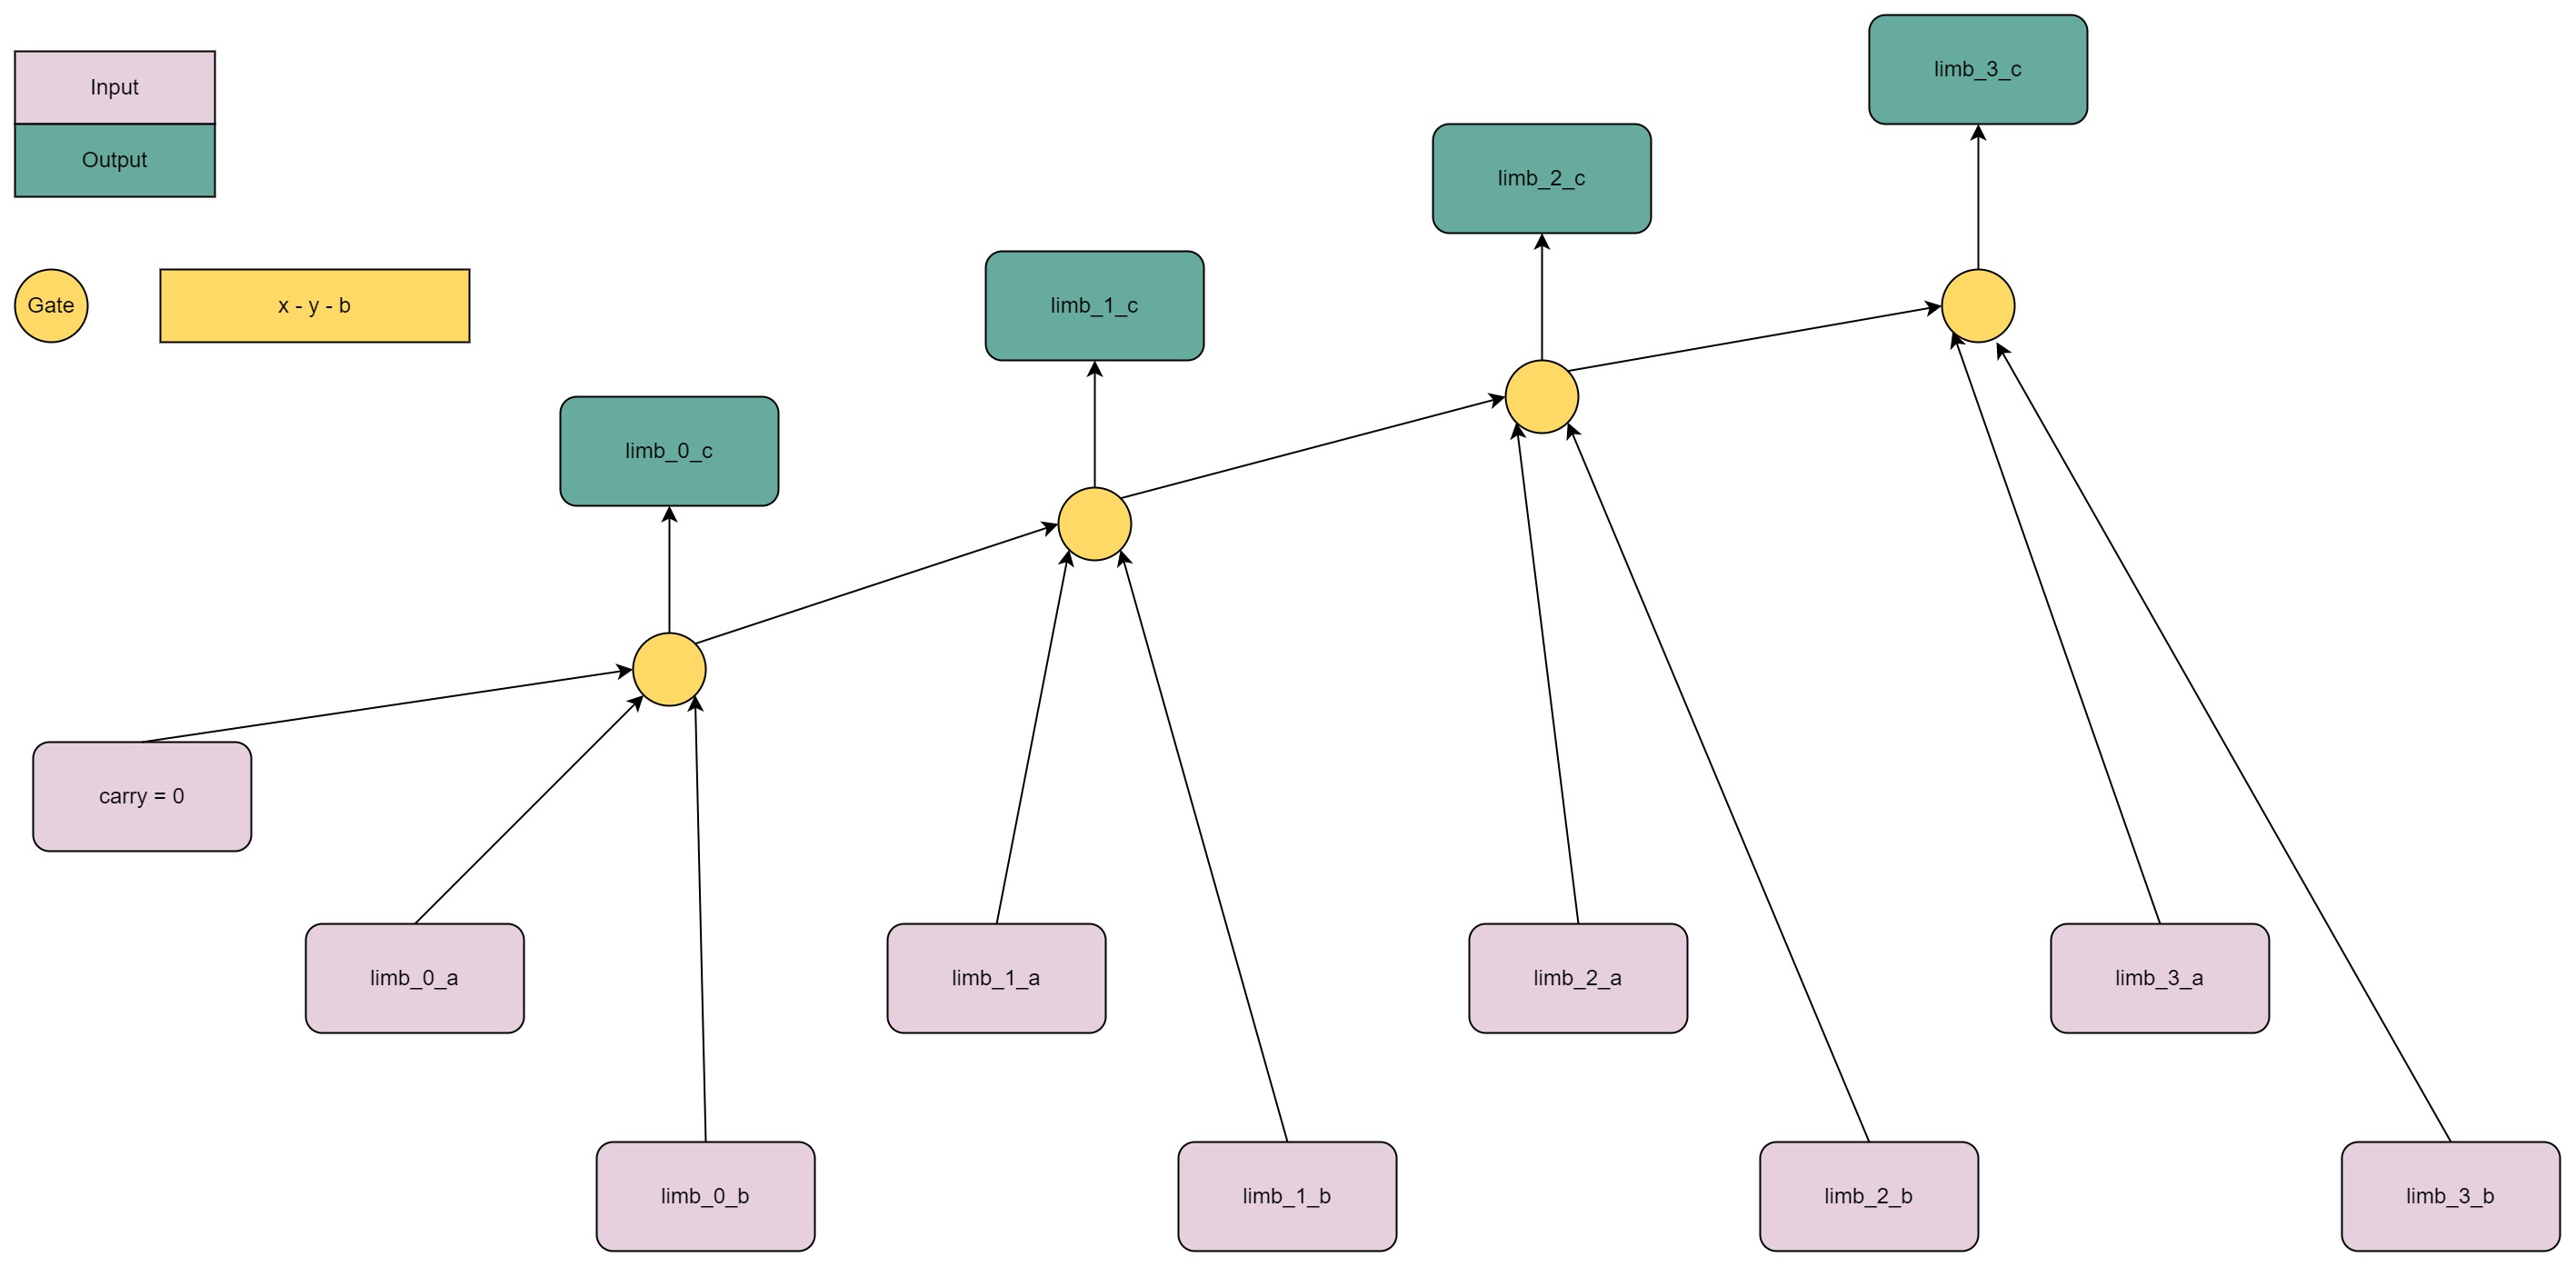
\includegraphics[width=0.8\textwidth]{biguint-sub-circuit-layout.jpg}
    \caption{biguint-sub circuit layout}
    \label{fig:biguint-sub-circuit-layout}
\end{figure}

\Par{Trace layout}
See \figref{fig:biguint-sub-trace-layout}.
\begin{figure}[!ht]
    \centering
    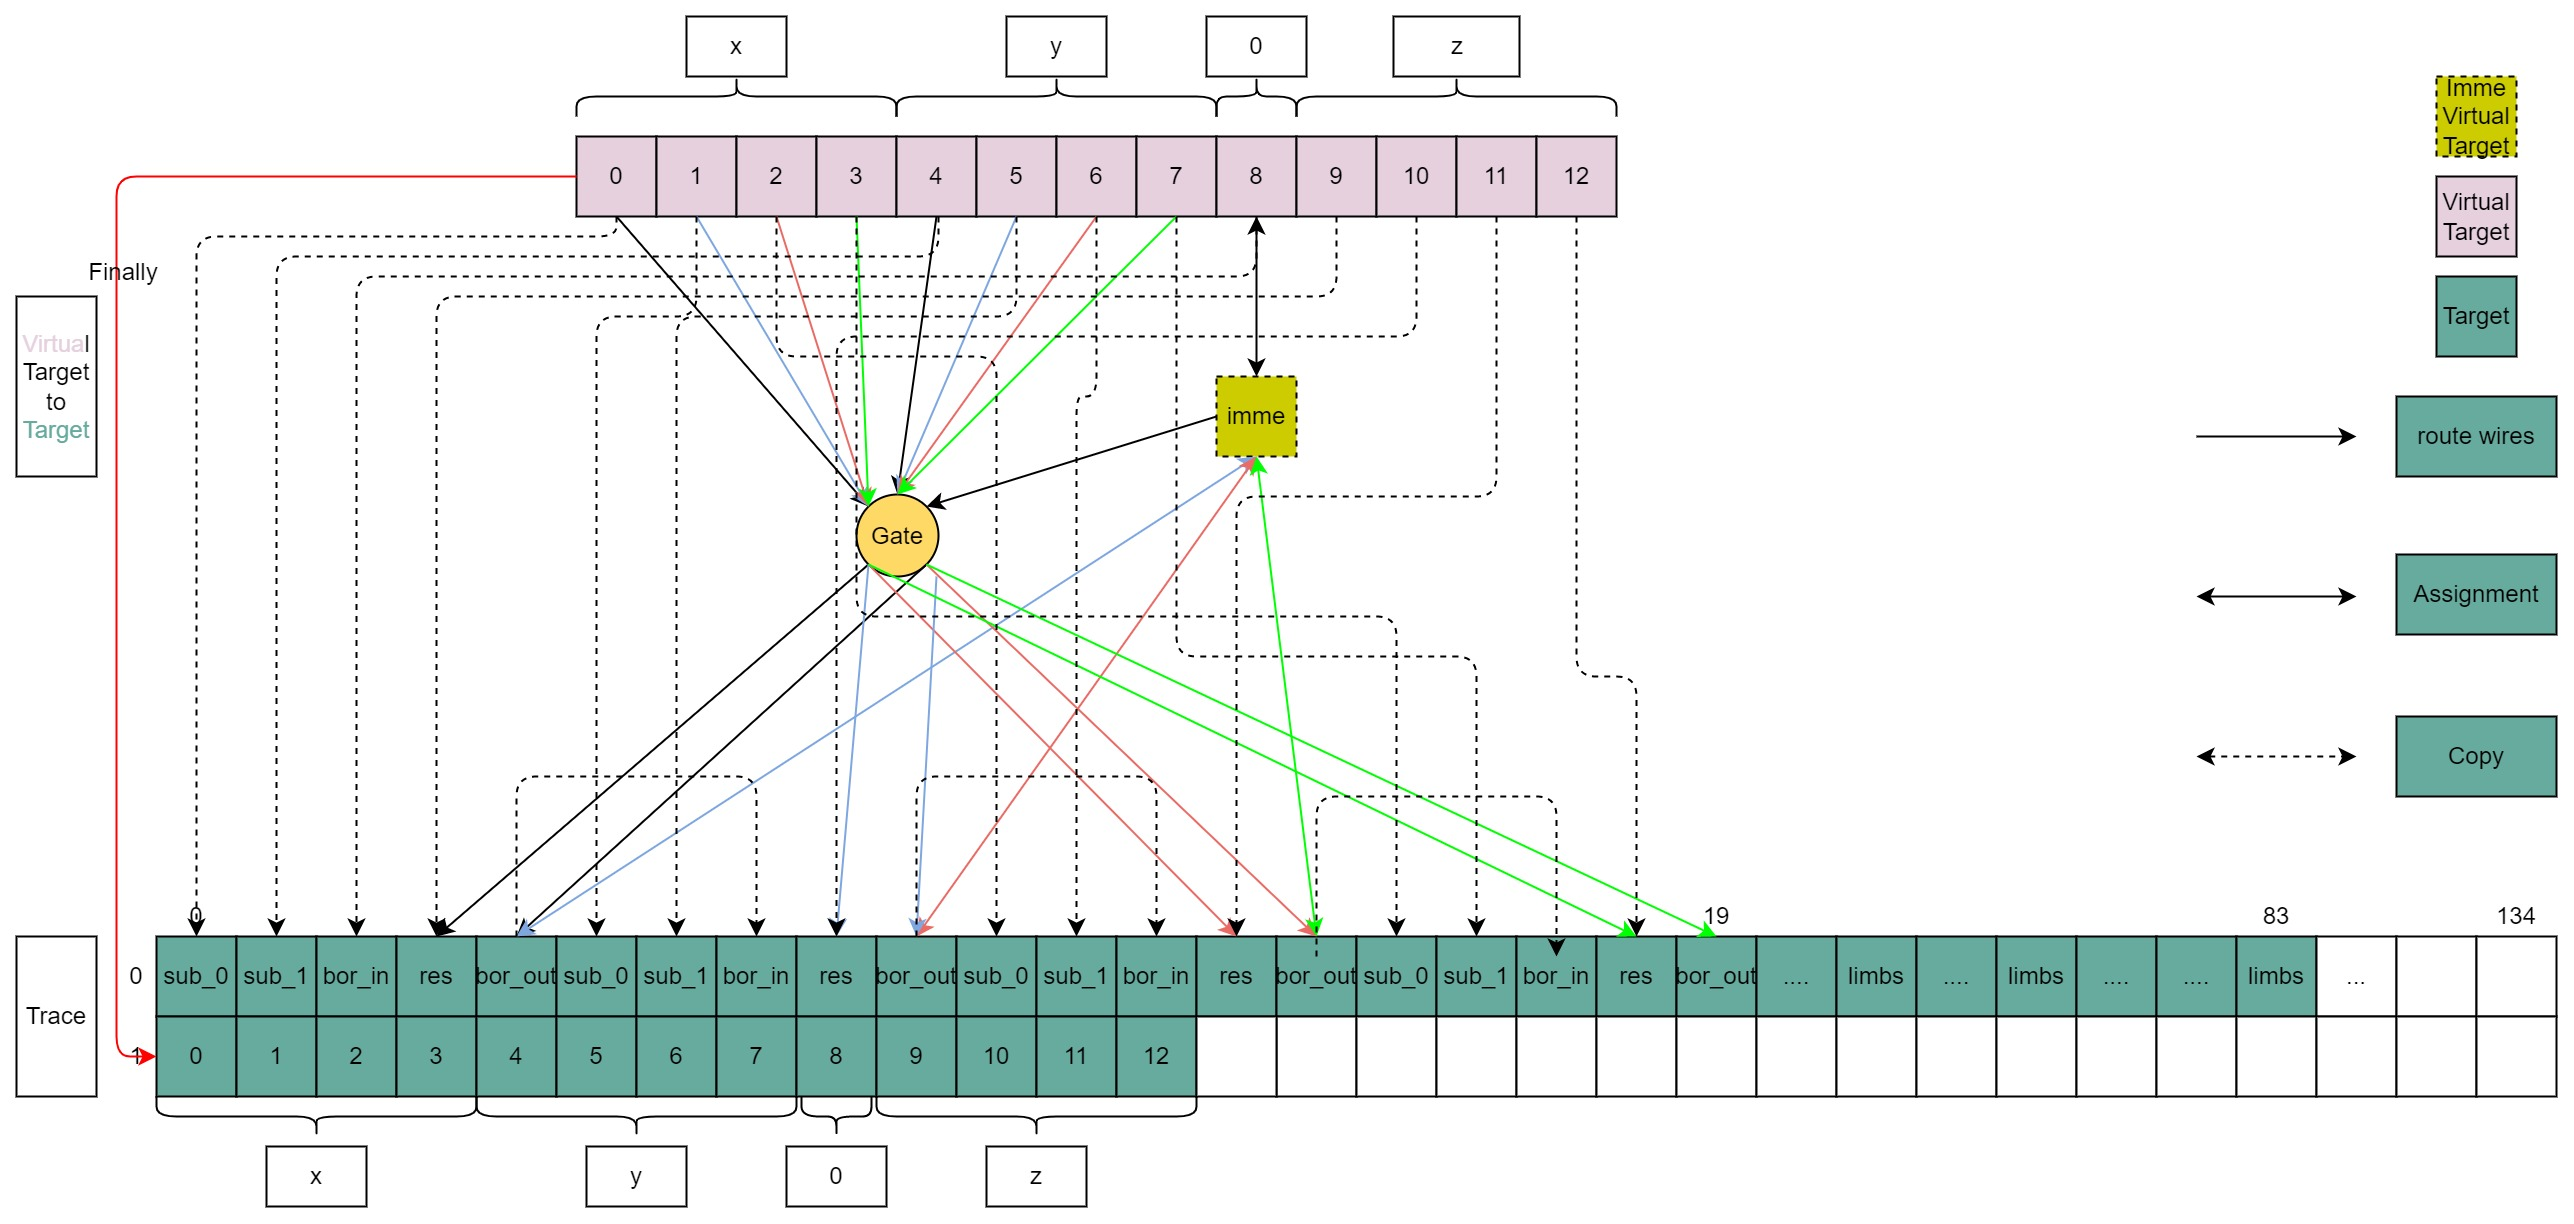
\includegraphics[width=0.8\textwidth]{biguint-sub-trace-layout.jpg}
    \caption{biguint-sub trace layout}
    \label{fig:biguint-sub-trace-layout}
\end{figure}

\Par{Constraints info and costs}
\begin{itemize}
    \item constraints-num: $6 \times (3 + 32 / 2) = 114$
    \item copy-constraints: $16$
    \item max-degree: $4$
    \item wires-num: $6 \times (5 + 16) = 126$
\end{itemize}

\Par{Questions}
\begin{itemize}
    \item Why not make rangecheck constraint for inputs?
    \item Could try to use the same constraint with add-gate.
\end{itemize}

    \subsubsection{biguint-mul}

\Par{Target}
Implement the multiplication of two biguints.

\Par{Constraints logic}
\begin{itemize}
    \item Compute mul-factors first, use U32ArithmeticGate;
    \item Add mul-factors from low bits, use U32AddManyGate.
\end{itemize}

\Par{Process layout}
See \figref{fig:biguint-mul-layout}
\begin{figure}[!ht]
    \centering
    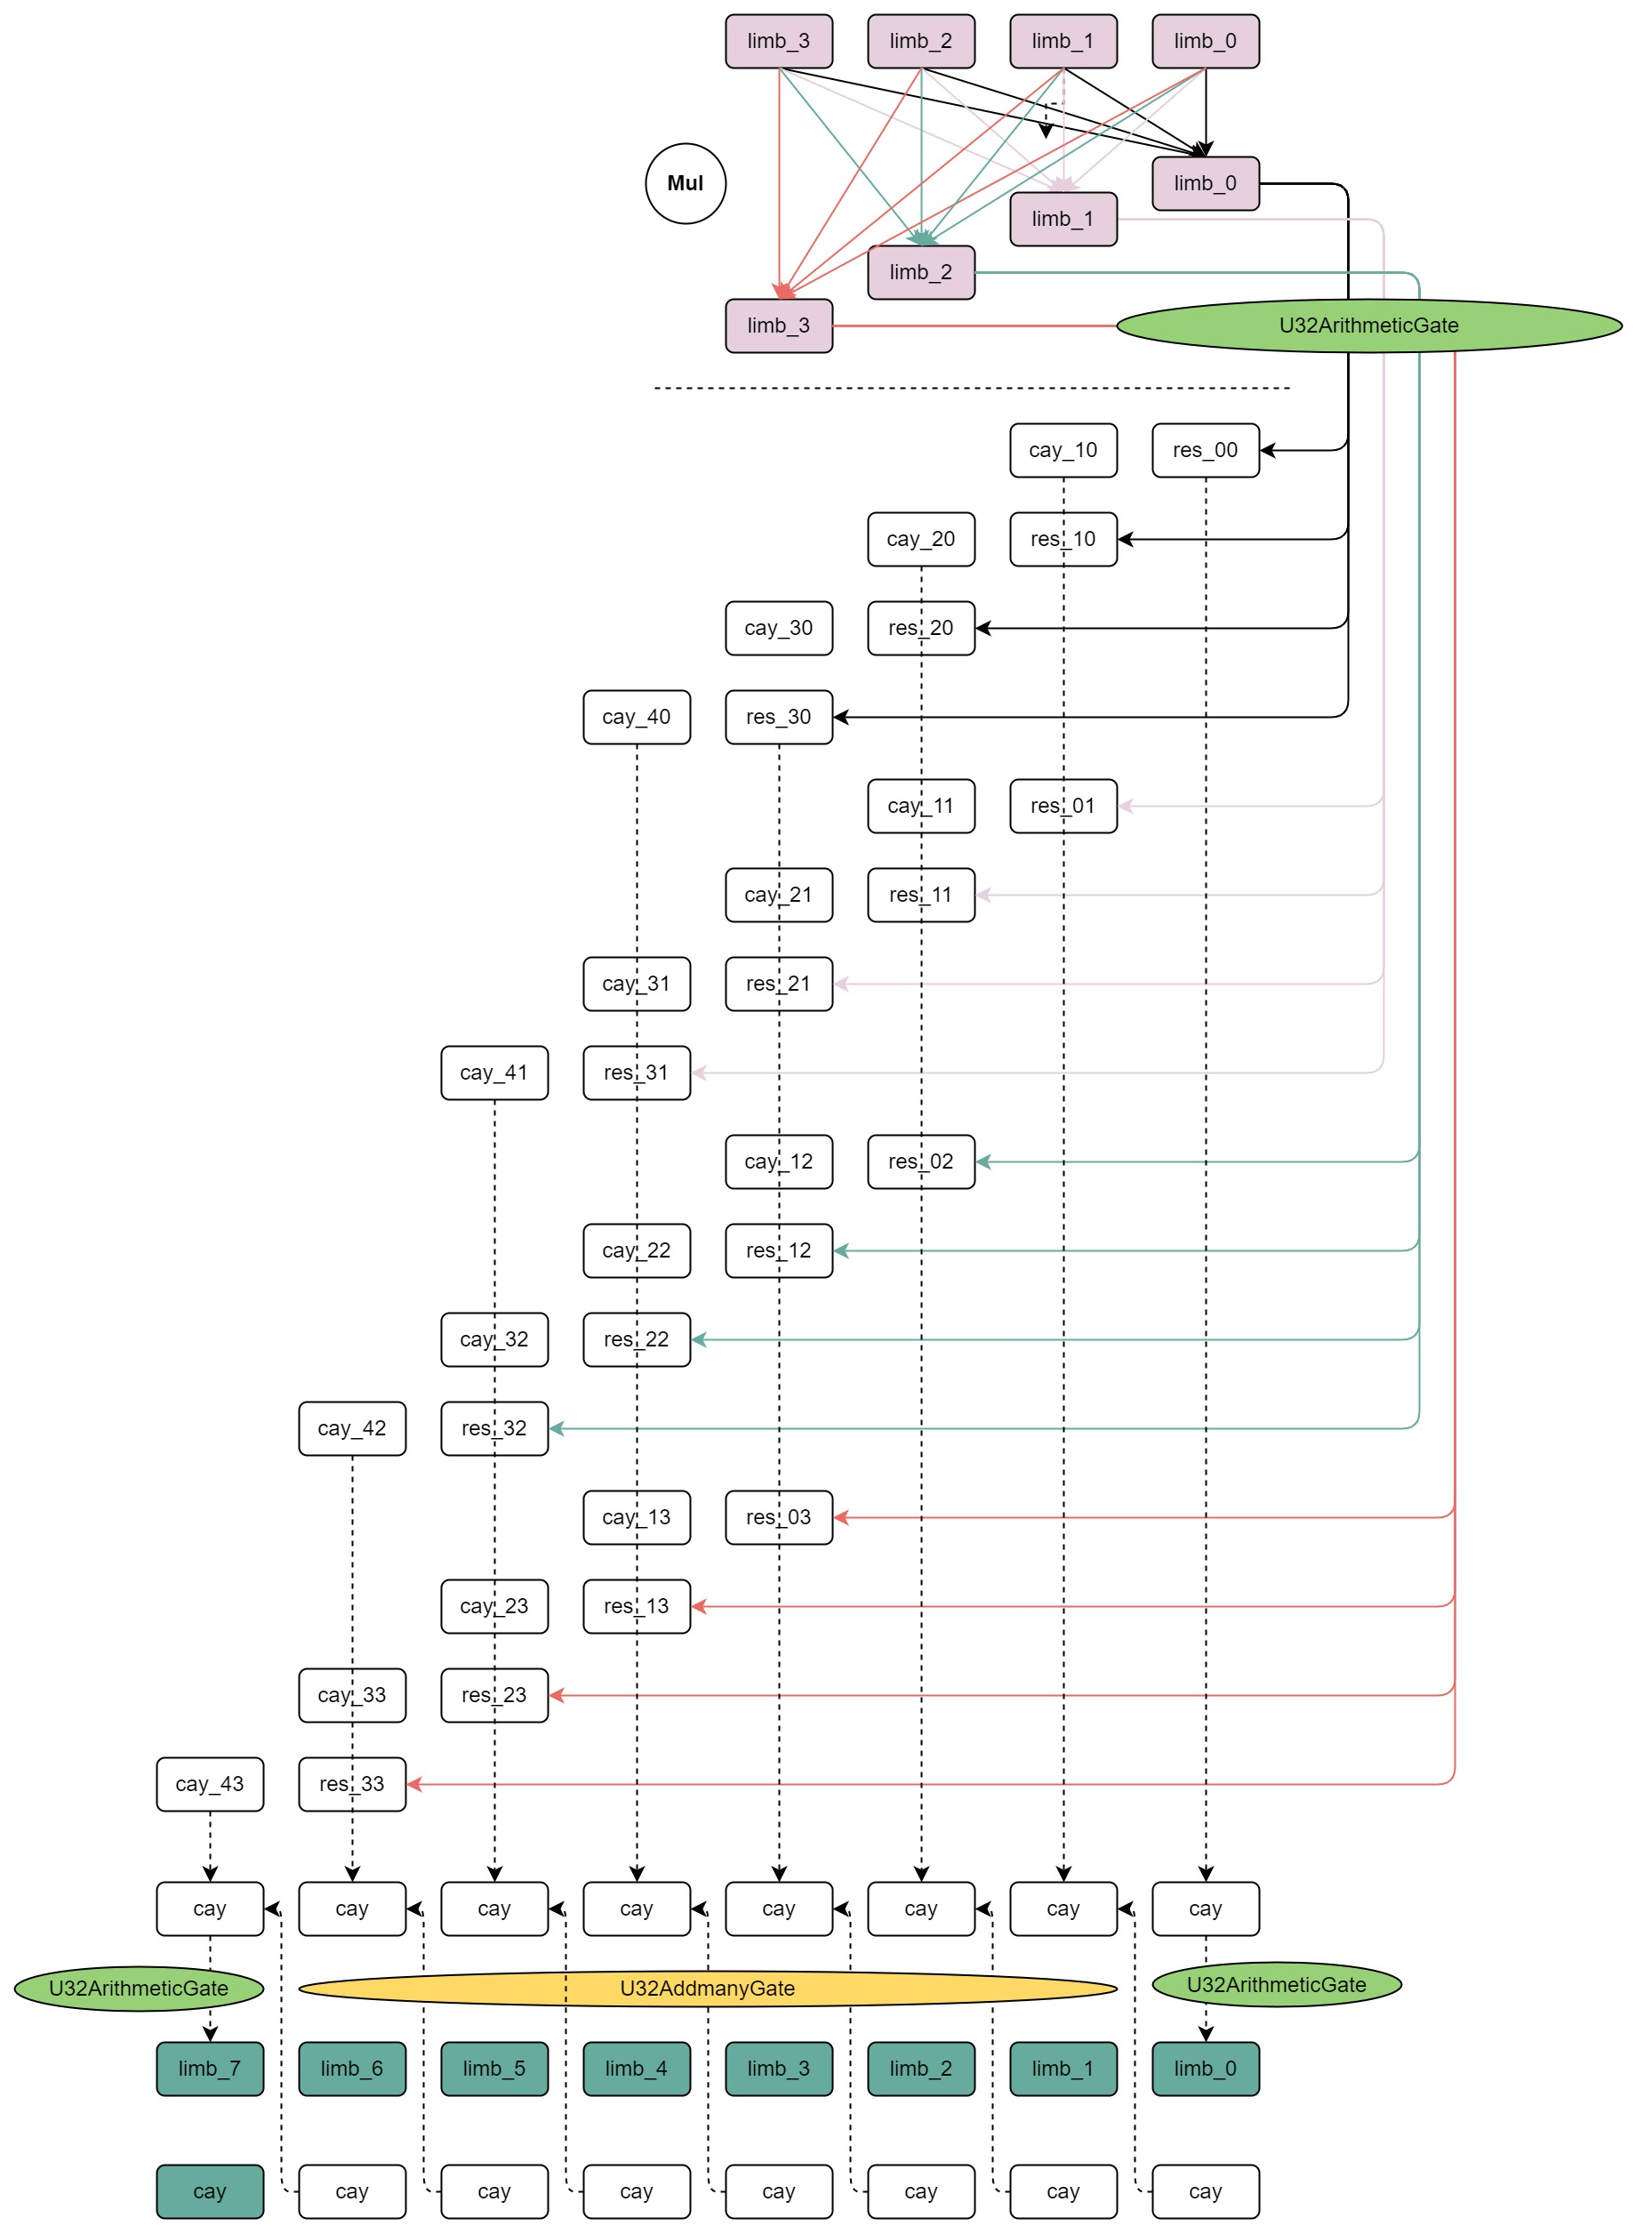
\includegraphics[width=0.8\textwidth]{biguint-mul-layout.jpg}
    \caption{biguint-mul layout}
    \label{fig:biguint-mul-layout}
\end{figure}

\Par{Constraints info and costs}
\begin{itemize}
    \item Gate type num: 4 (U32ArithmeticGate, U32AddManyGate(num-addends: 4), U32AddManyGate(num-addends: 6), U32AddManyGate(num-addends: 8))
    \item Gate instance num: 9
    \item U32ArithmeticGate num: 6
    \item U32AddManyGate num: 3
    \item copy-constraints: $18 \times 3 + (4 + 6 + 8) \times 2 + 9 = 99$
    \item max-degree: 4
\end{itemize}

    \section{biguint-div}
\label{biguint-div}

Note that div-rem has the same constraints logic with div

\begin{enumerate}
    \item target
        \begin{itemize}
            \item implement the division of two biguints
        \end{itemize}
    \item constraints-logic
        \begin{itemize}
            \item not implement div-algrithem directly
            \item use nondeterministic feature to check div-logic
            \item check div * b + rem = a
            \item check rem < b
        \end{itemize}
    \item div-process layout
        \begin{figure}[!ht]
            \centering
            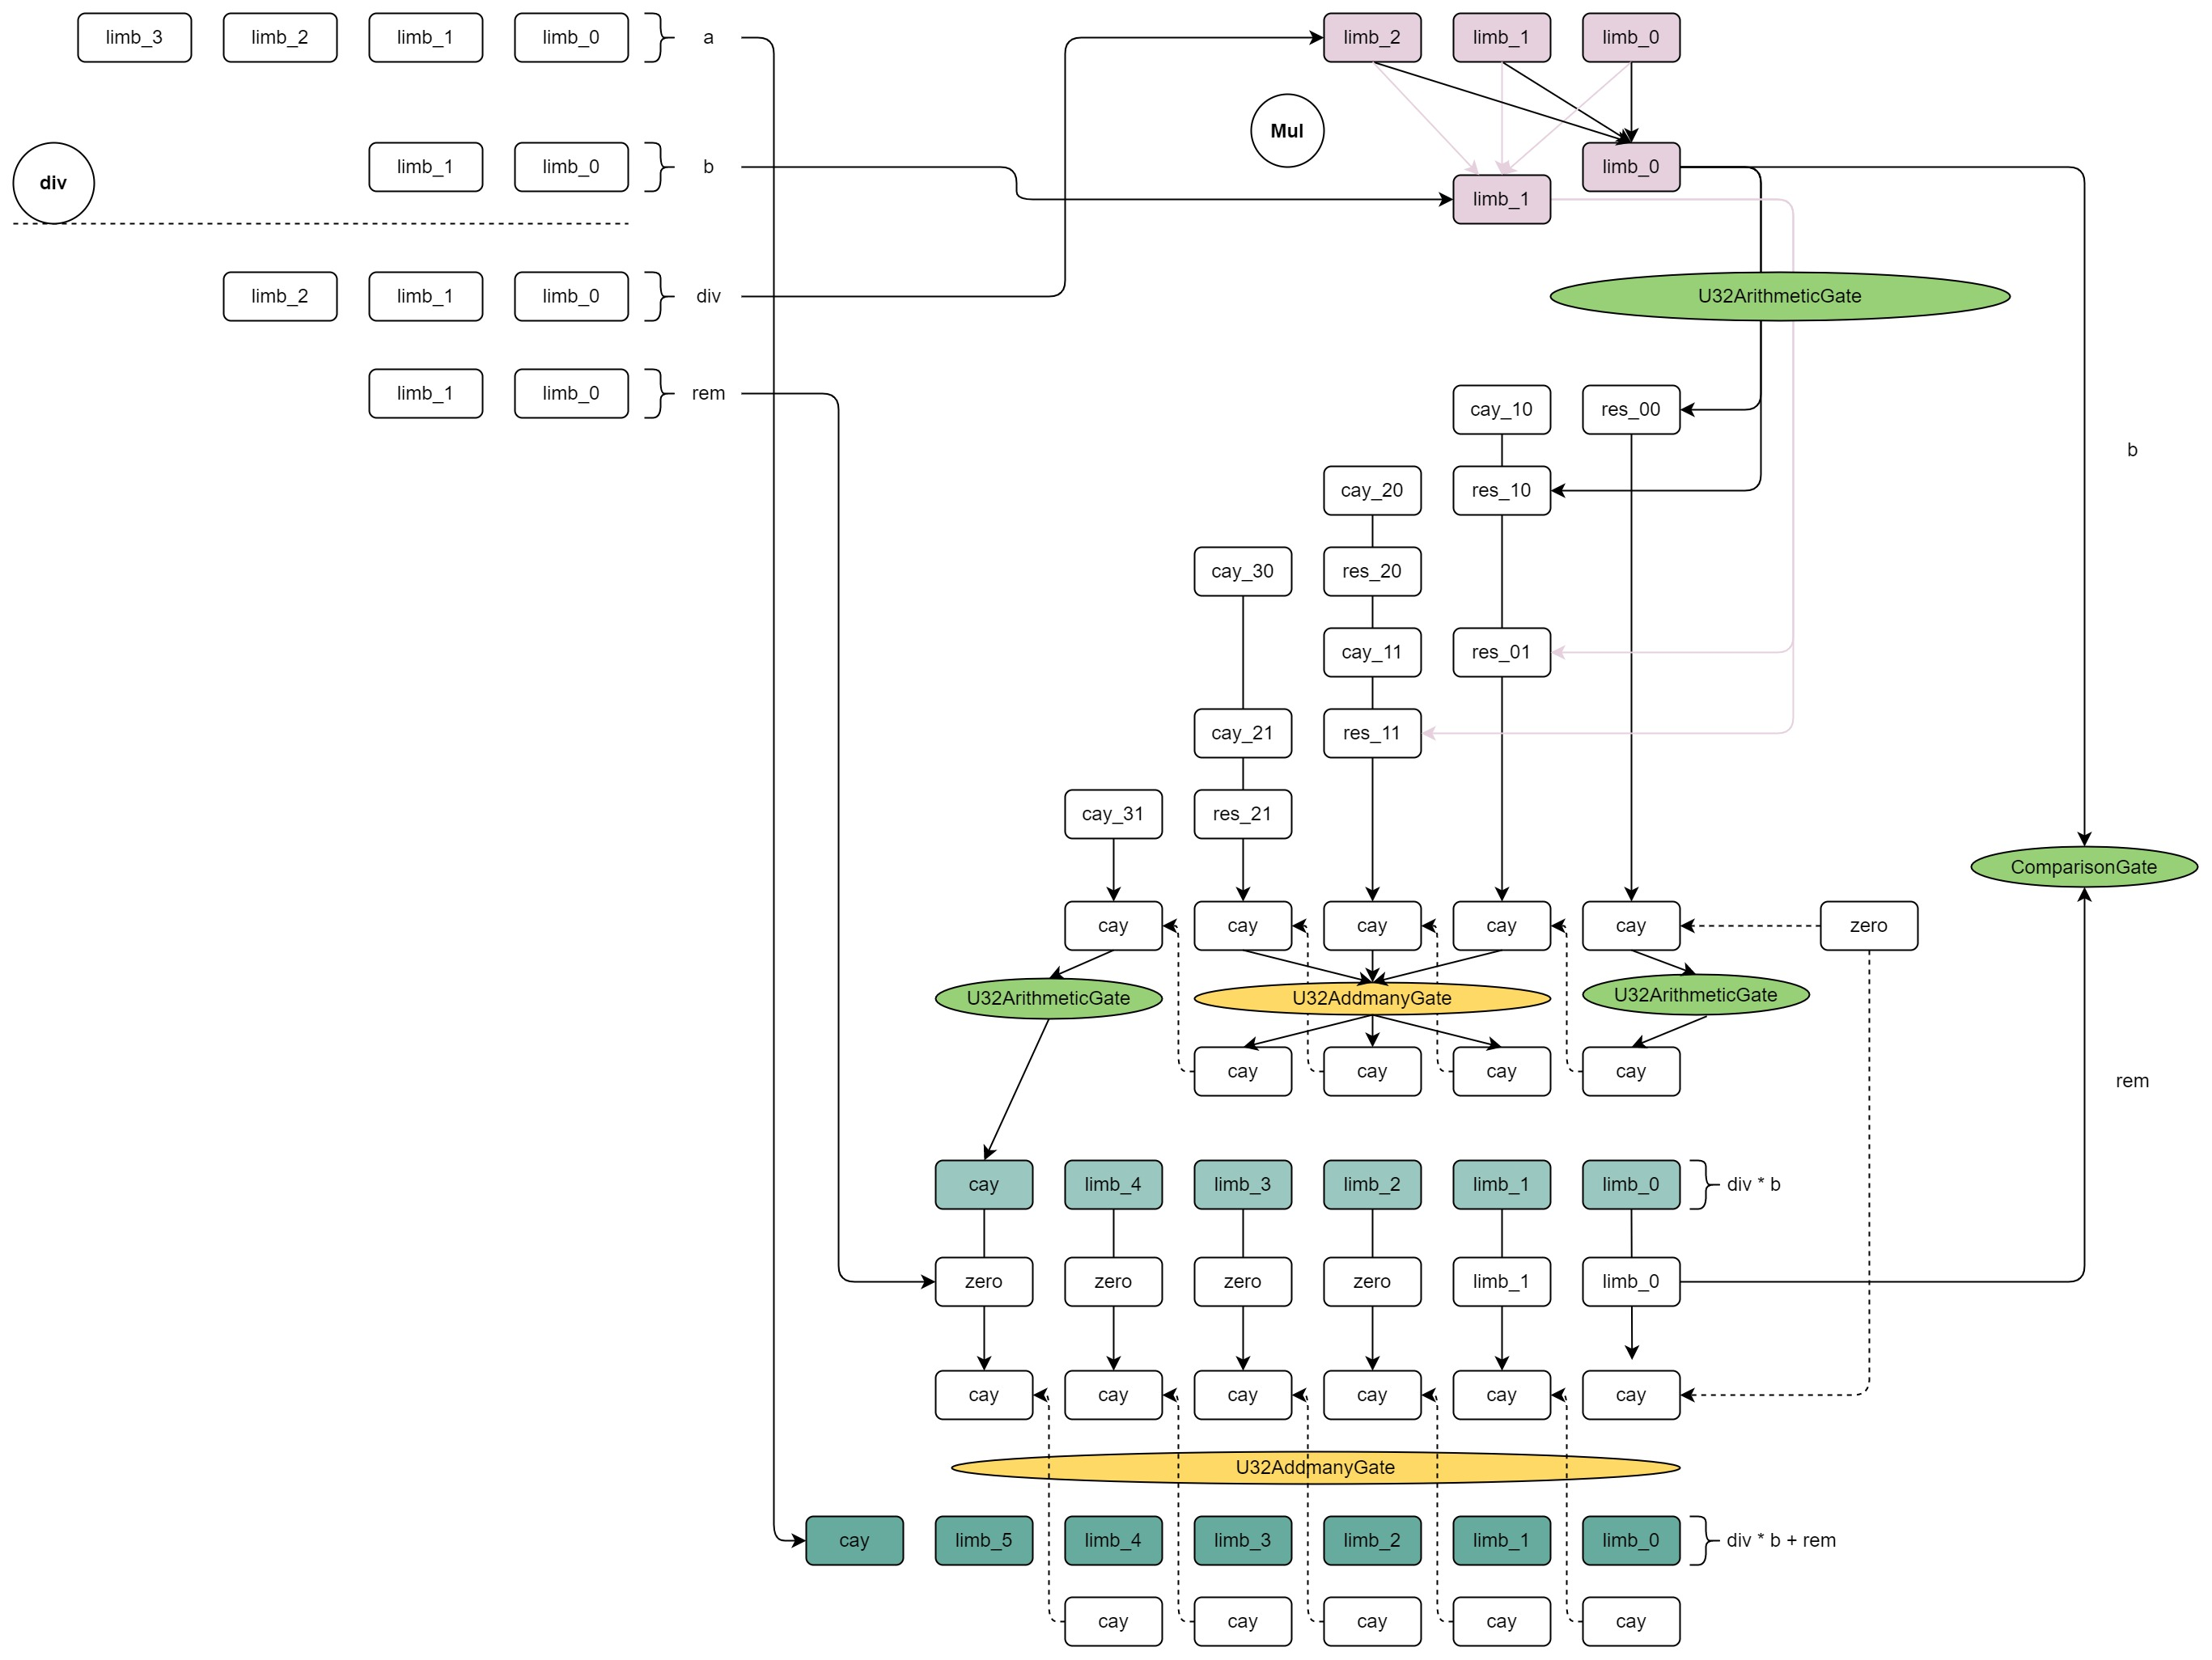
\includegraphics[width=0.8\textwidth]{biguint-div-layout.jpg}
            \caption{biguint-div layout.jpg}
            \label{fig:biguint-div-layout.jpg}
        \end{figure}
    
    \item constraints-info and costs
        \begin{itemize}
            \item Gate type num: 5(U32ArithmeticGate, U32AddManyGate(num-addends: 3), U32AddManyGate(num-addends: 4), ComparisionGate, ArithmeticGate)
            \item Gate instance num: 3 + 3 + 4 + 3 = 13 
            \item U32ArithmeticGate num: 3
            \item U32AddManyGate num: 3
            \item ComparisionGate num: 4
            \item ArithmeticGate num: 3
            \item copy-constraints: 3 * 8 + 4 + 5 + 4 + 4 * 6 + 7 + 1 + 26 + 5 = 100 
            \item max-degree: 4
        \end{itemize}

\end{enumerate}
    \subsubsection{biguint-cmp}

\Par{Target}
Implement the comparison of two biguints.

\Par{Constraints logic}
\begin{itemize}
    \item Split the input to many limbs, such that: \verb|limbs_num = bits / chunks|;
    \item Execute comparison for low bits limbs;
    \item Ensure that the result is determined by the highest limbs which are not equal.
\end{itemize}

\Par{Process layout}
See \figref{fig:biguint-cmp-layout}.
\begin{figure}[!ht]
    \centering
    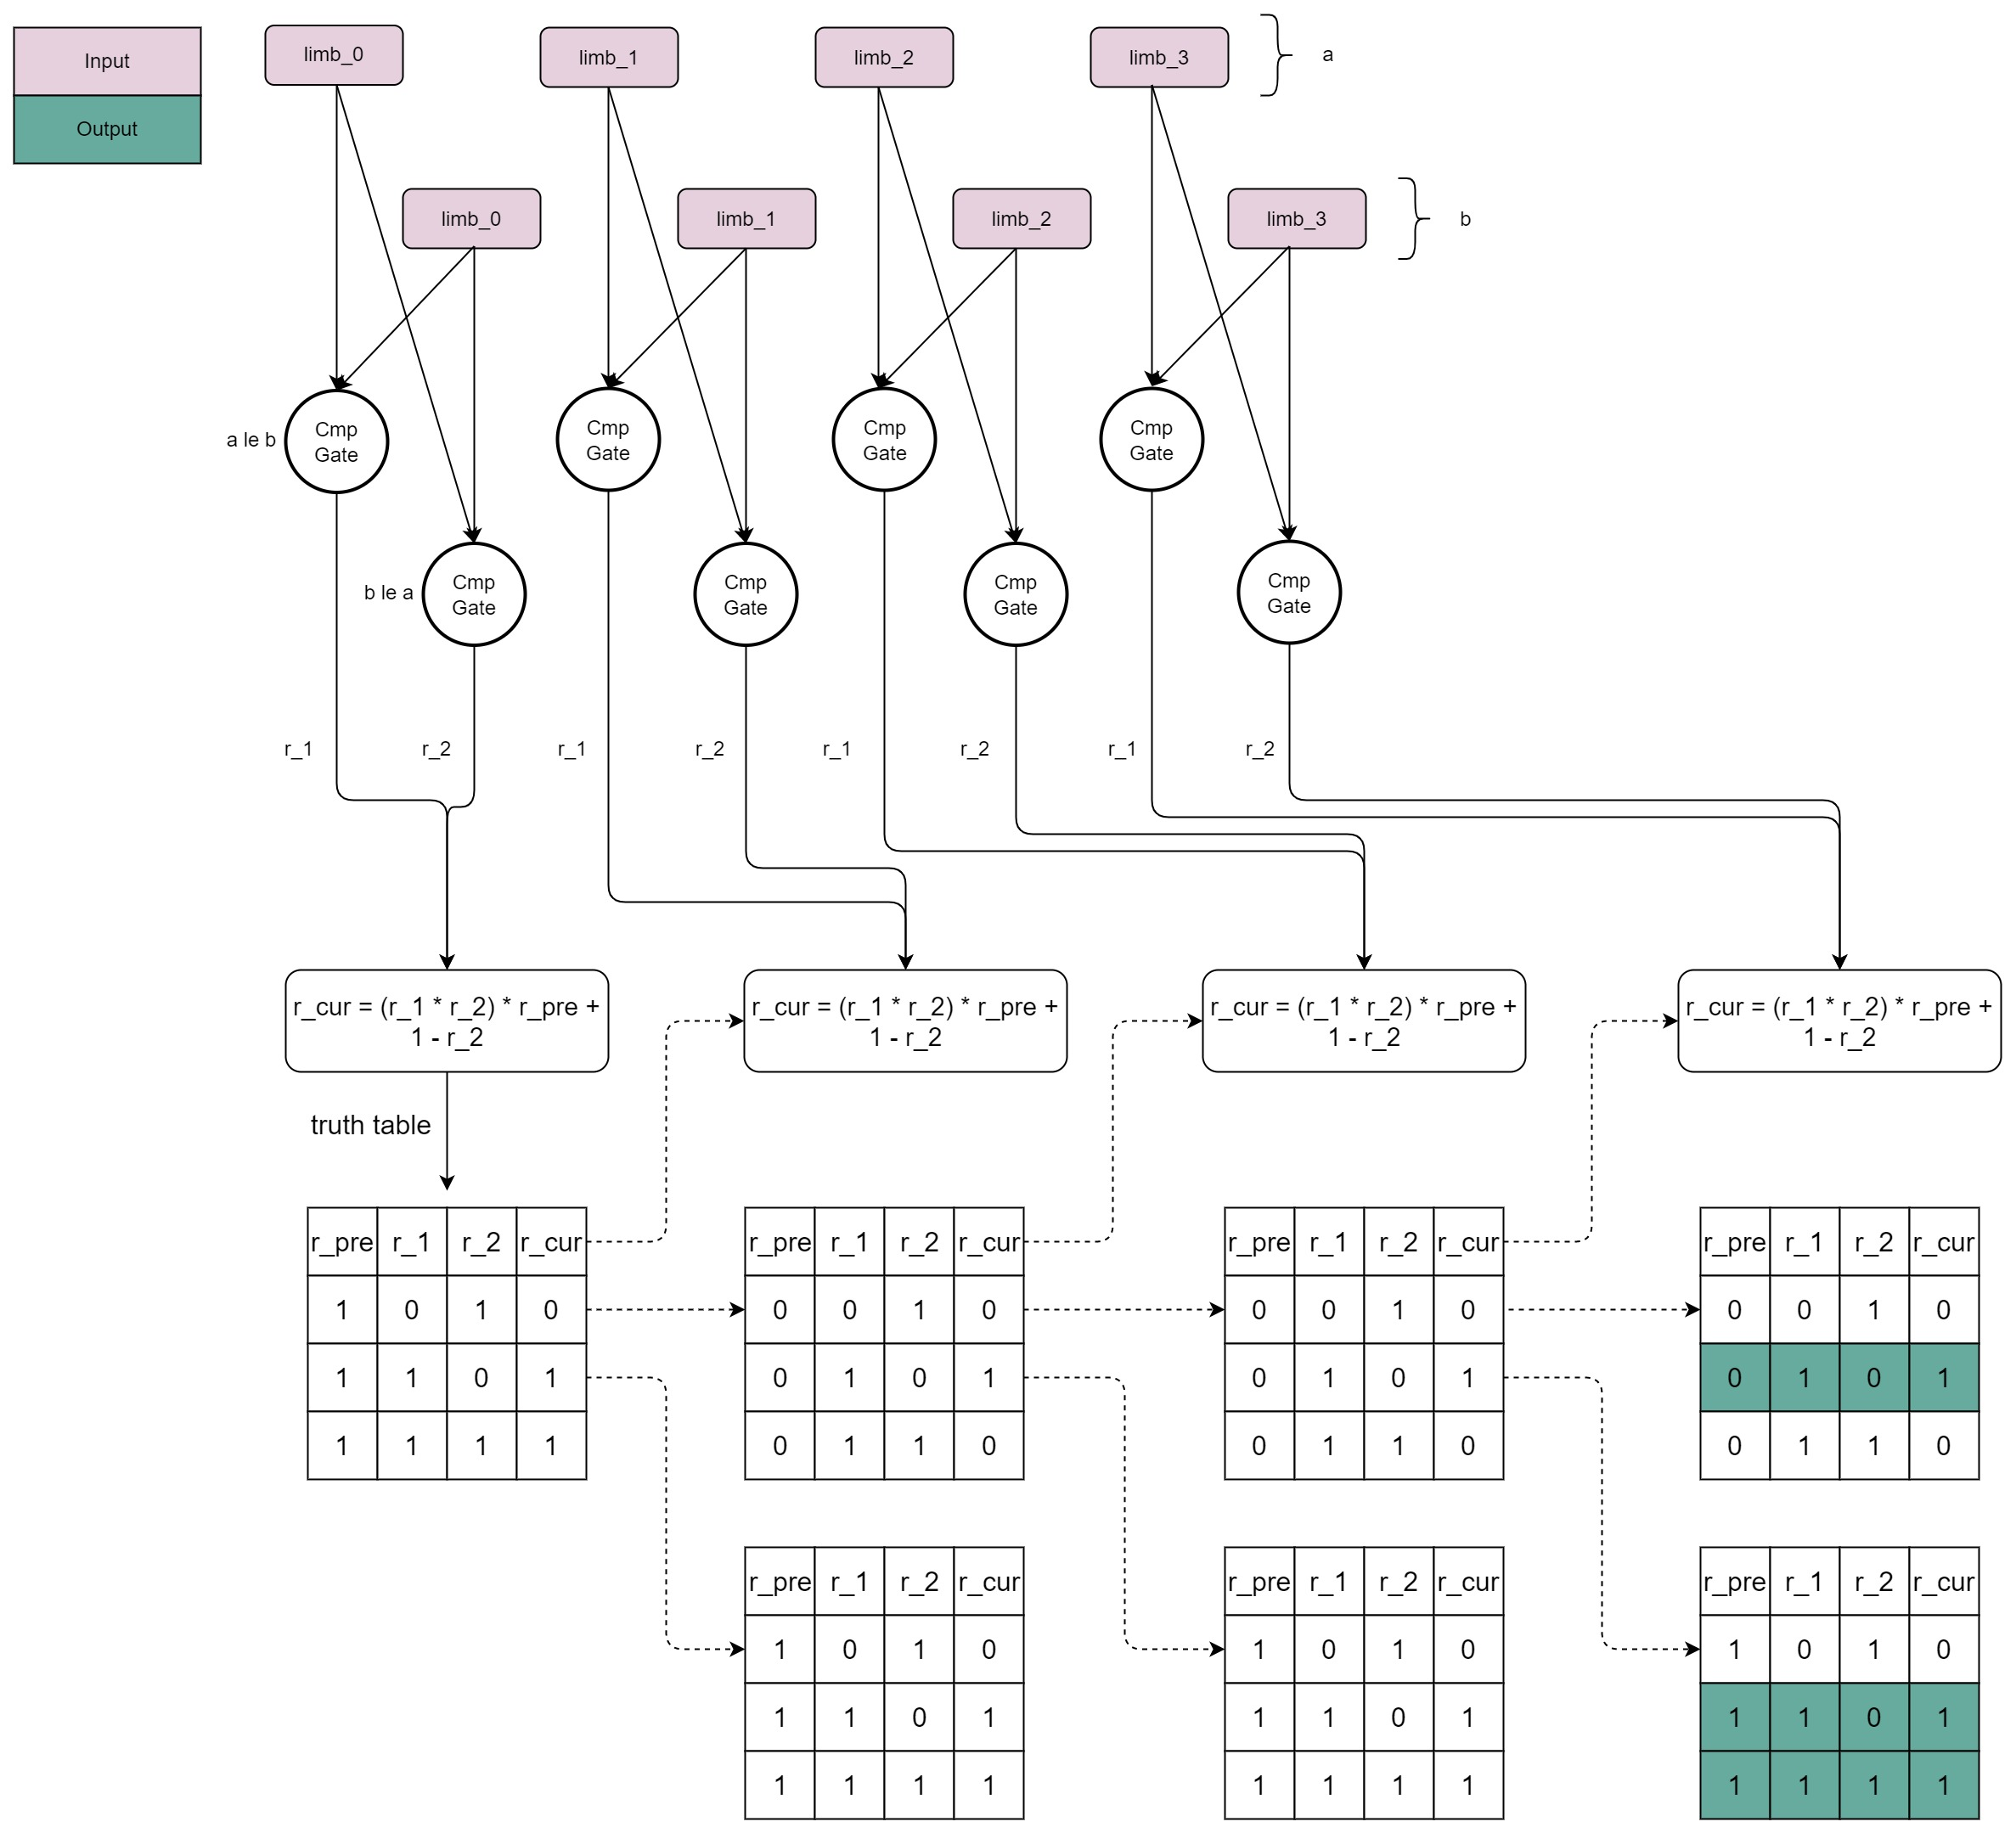
\includegraphics[width=0.8\textwidth]{biguint-cmp-layout.jpg}
    \caption{biguint-cmp layout}
    \label{fig:biguint-cmp-layout}
\end{figure}

\Par{Circuit layout}
See \figref{fig:biguint-cmp-circuit-layout}.
\begin{figure}[!ht]
    \centering
    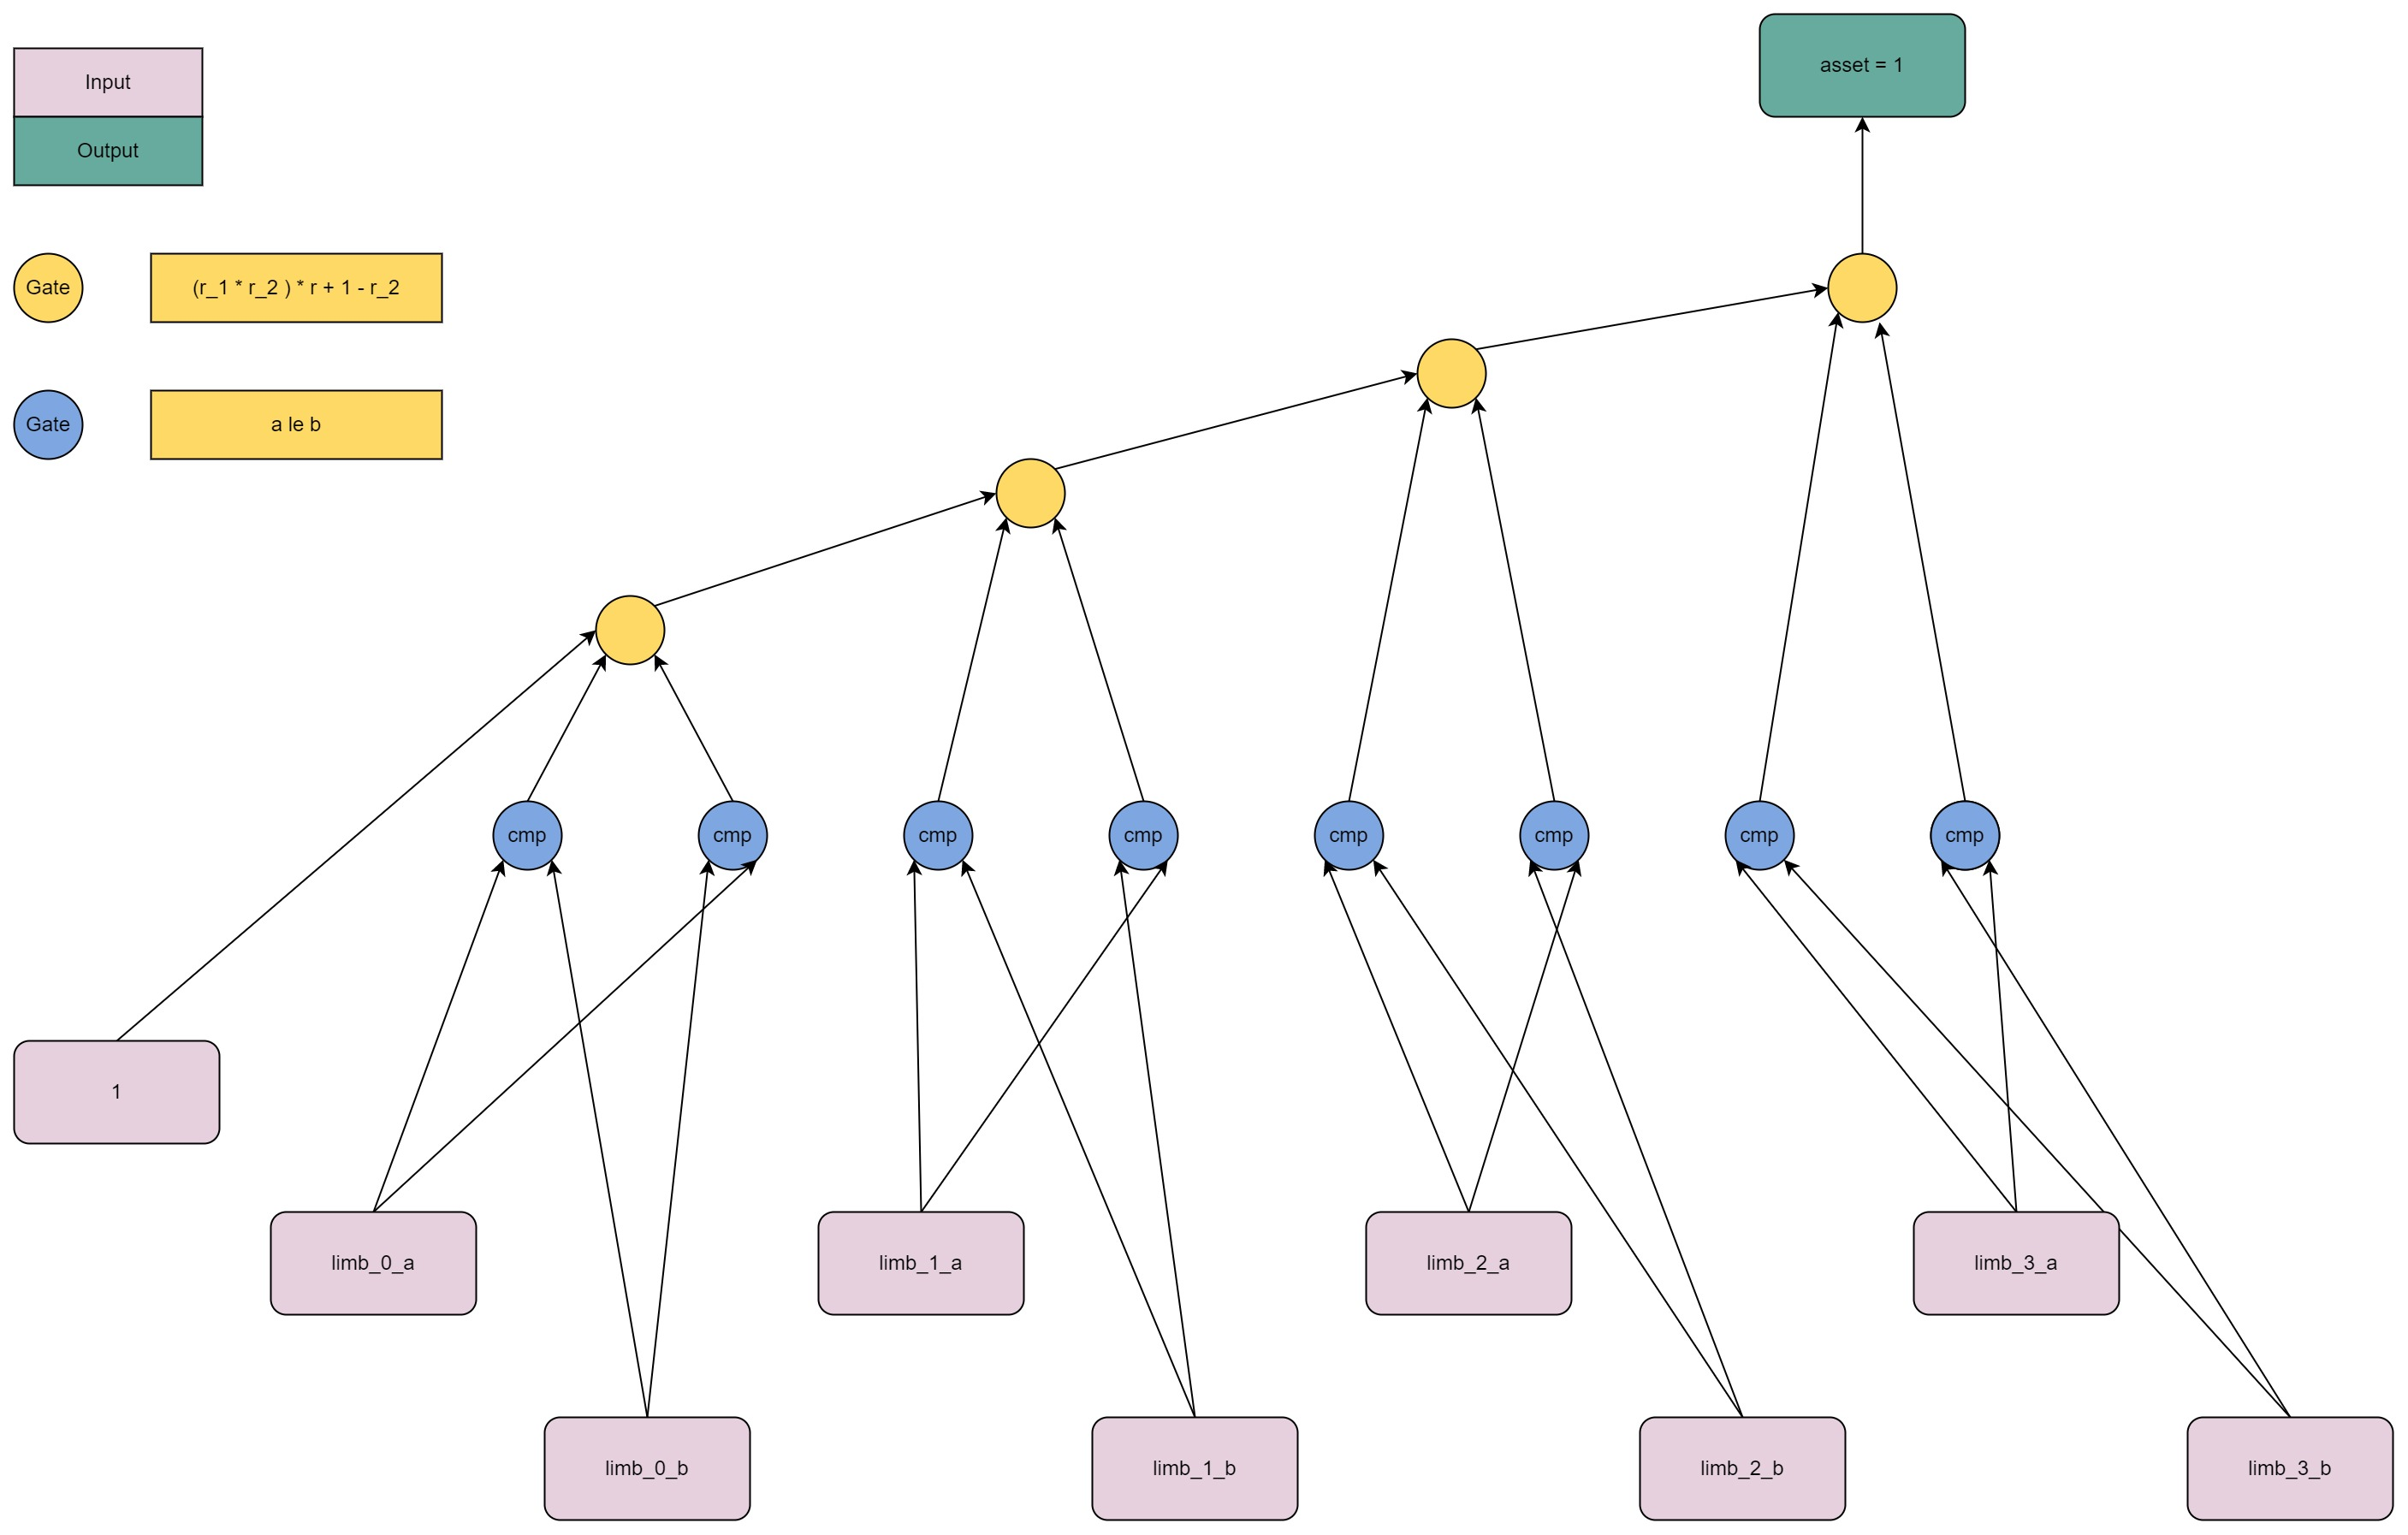
\includegraphics[width=0.8\textwidth]{biguint-cmp-circuit-layout.jpg}
    \caption{biguint-cmp circuit layout}
    \label{fig:biguint-cmp-circuit-layout}
\end{figure}

\Par{Constraints info and costs}
\begin{itemize}
    \item Gate type num: 2 (ComparisionGate, ArithmeticGate)
    \item Gate instance num: $4 \times 2 + 3 = 11$
    \item ComparisionGate num: 8
    \item ArithmeticGate num: 3
    \item copy-constraints: $(4 + 9) \times 4 + 1 = 53$
    \item max-degree: 4
\end{itemize}

    \subsubsection{nonnative-add}
\label{nonnative-add}

\begin{enumerate}
    \item target
        check the additional relation among three nonnative target objects.
    \item constraints-logic
        \begin{itemize}
            \item check equation for gadget,  a + b = c + modular * overflow
            \item check that "c lt modular"
        \end{itemize}
    \item nonnative-add process layout
        \begin{figure}[!ht]
            \centering
            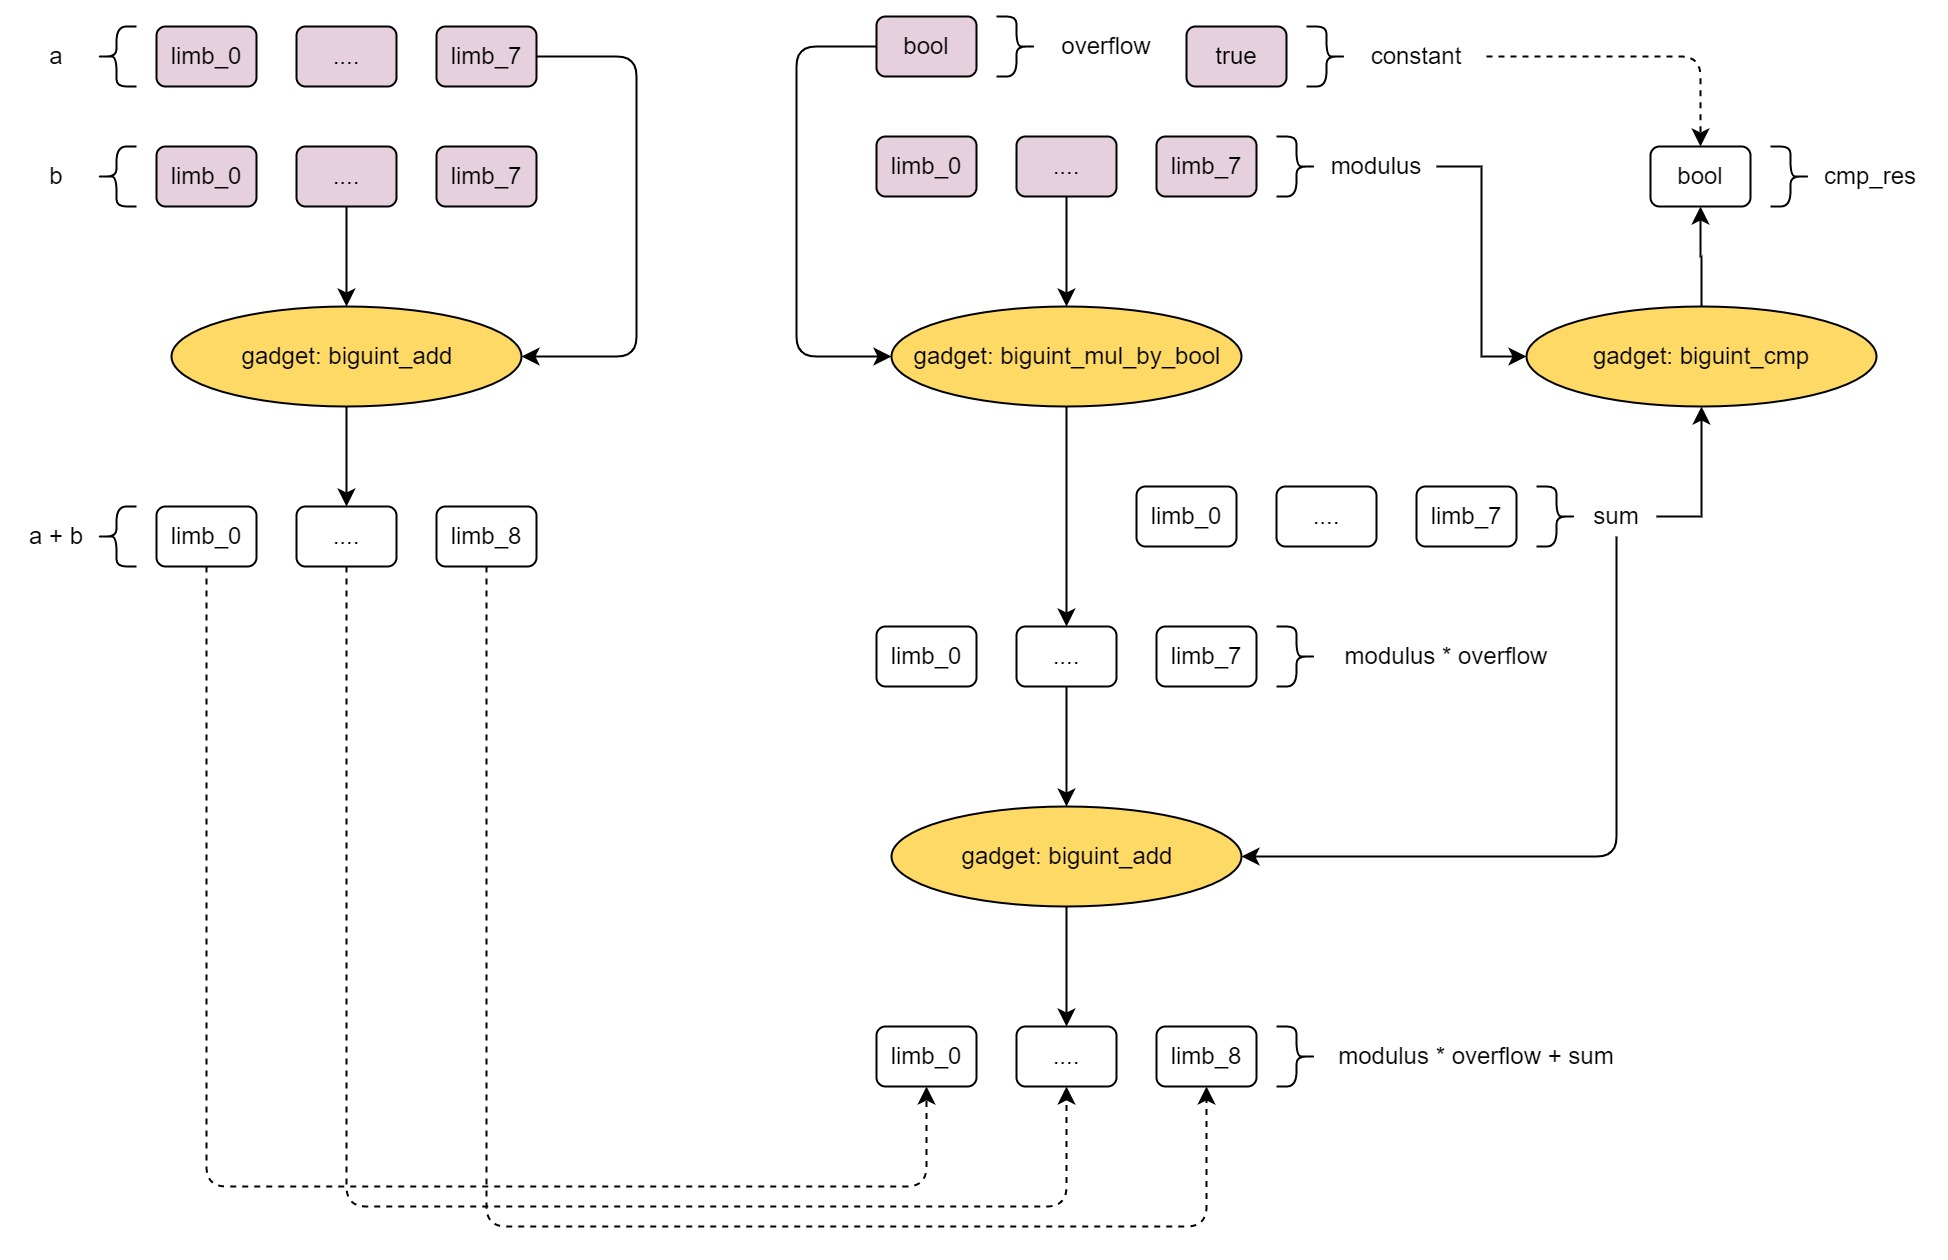
\includegraphics[width=0.8\textwidth]{nonnative-add-layout.jpg}
            \caption{nonnative-add layout}
            \label{fig:nonnative-add-layout}
        \end{figure}
    
    \item constraints-info and costs
        \begin{itemize}
            \item gadget biguint-add num: 2
            \item gadget biguint-mul-by-bool num: 1
            \item gadget biguint-cmp num: 1
            \item gate type num: 3(U32AddManyGate, ComparisonGate, ArithmeticGate)
            \item gate instance num: 23 = 3(U32AddManyGate) + 16(ComparisonGate) + 2(ArithmeticGate(1,0)) + 1(ArithmeticGate(1,-1)) + 1(ArithmeticGate(1,1))
            \item copy-constraints: 186 = 32 * 2{biguint-add} + 9{biguint-mul-by-bool} + 9 + (4 + 9) * 8{biguint-cmp} = 186
        \end{itemize}

    \item questions
        \begin{itemize}
            \item when set value to sum?
        \end{itemize}

\end{enumerate}
    \subsubsection{nonnative-sub}
\label{nonnative-sub}

\begin{enumerate}
    \item target
        check the substract relation among three nonnative target objects.
    \item constraints-logic
        \begin{itemize}
            \item check equation for gadget,  diff + b = a + modular * overflow
            \item check that "overflow is bool"
            \item check that "diff.limbs is range U32"
        \end{itemize}
    \item nonnative-sub process layout
        \begin{figure}[!ht]
            \centering
            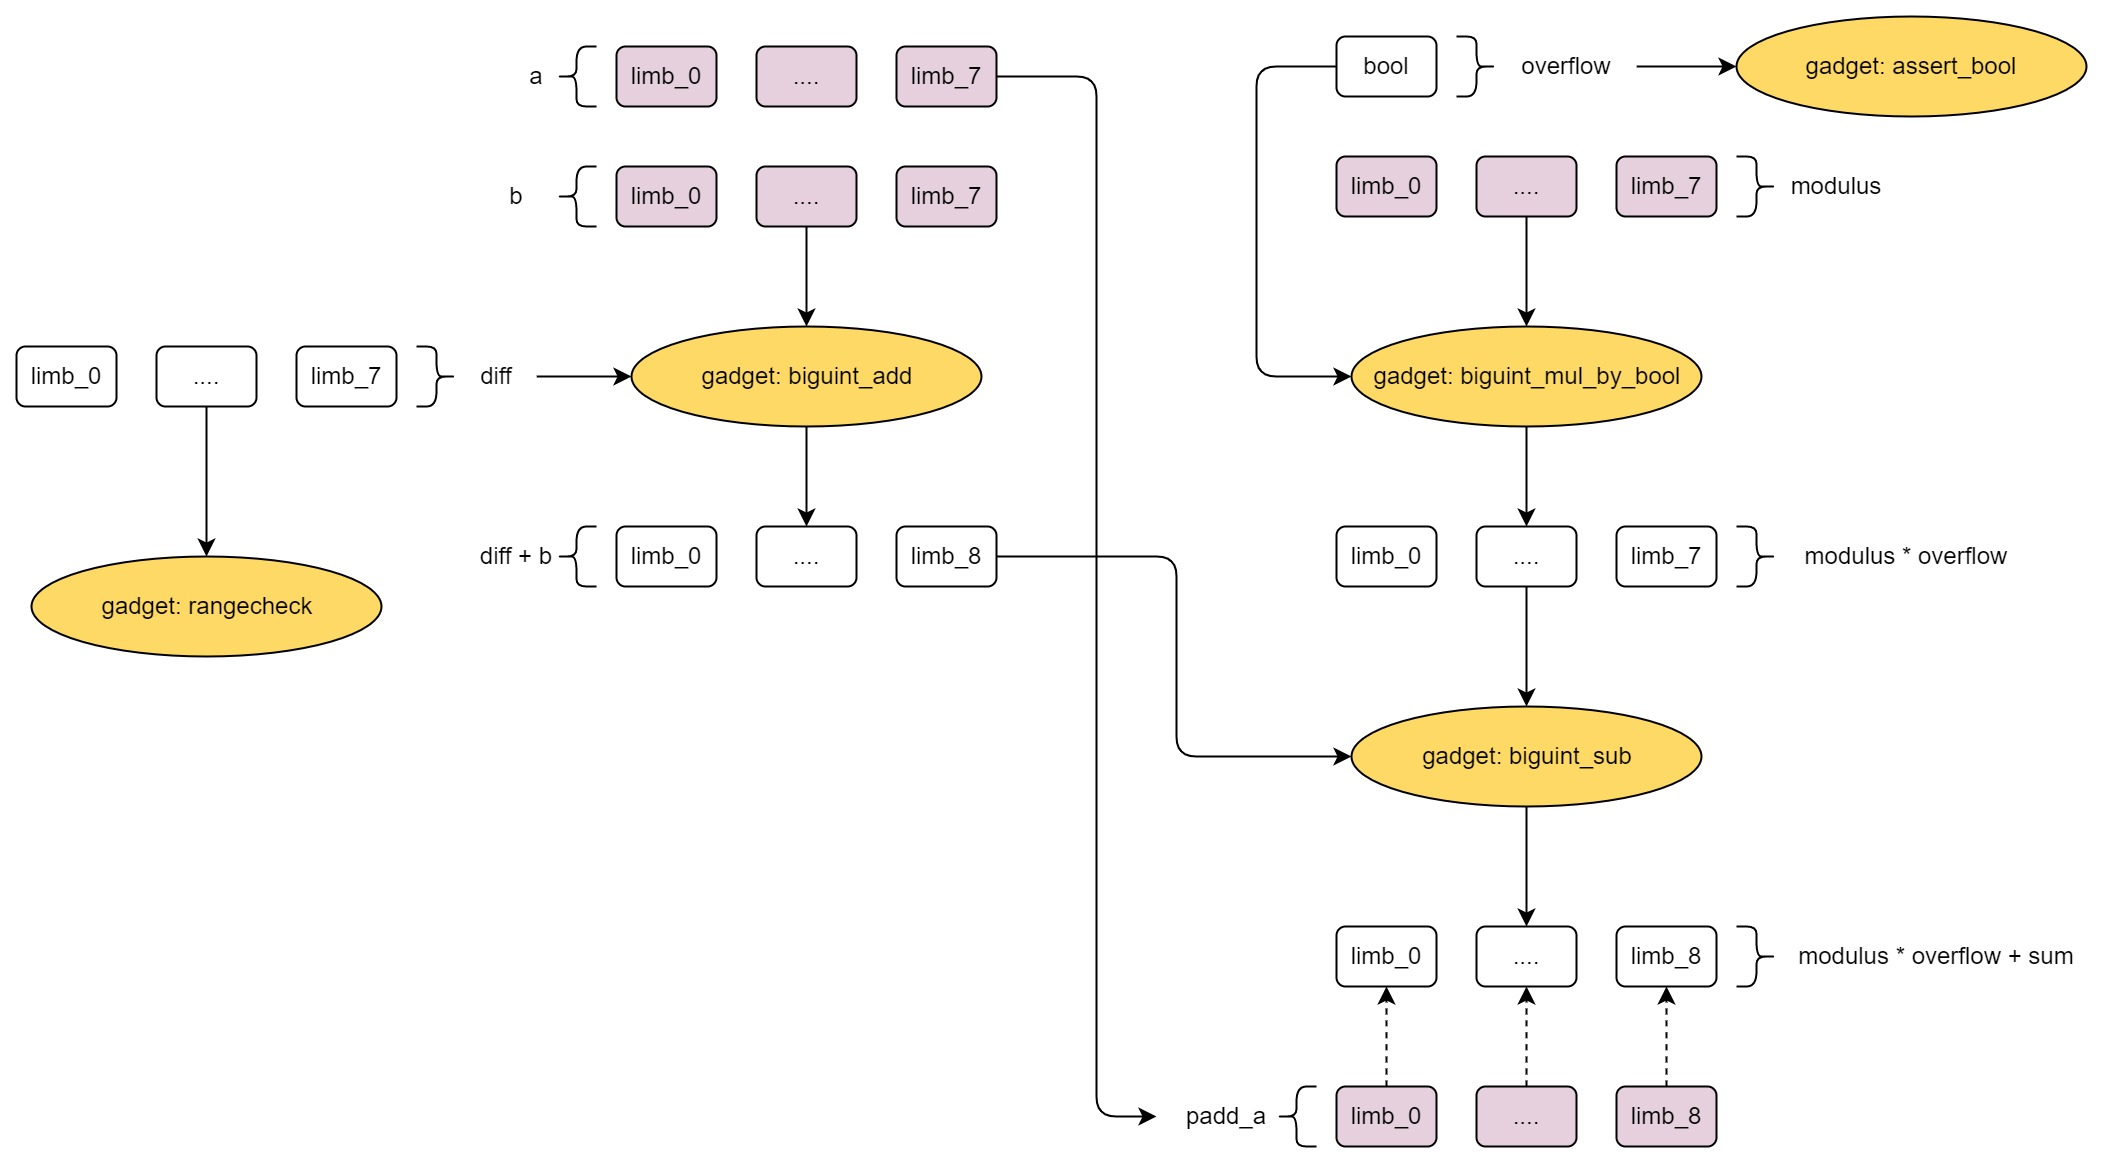
\includegraphics[width=0.8\textwidth]{nonnative-sub-layout.jpg}
            \caption{nonnative-sub layout}
            \label{fig:nonnative-sub-layout}
        \end{figure}
    
    \item constraints-info and costs
        \begin{itemize}
            \item gadget biguint-add num: 1
            \item gadget biguint-sub num: 1
            \item gadget biguint-mul-by-bool num: 1
            \item gadget u32rangecheck num: 1
            \item gadget assert-bool num: 1
            \item gate type num: 4(U32AddManyGate, U32SubtractionGate, U32RangeCheckGate, ArithmeticGate)
            \item gate instance num: 7 = 2(U32AddManyGate) + 2(U32SubtractionGate) + 1(U32RangeCheckGate) + 1(ArithmeticGate(1,0)) + 1(ArithmeticGate(1,-1))
            \item copy-constraints: 89 = 32{biguint-add num} + 27{U32SubtractionGate} + 9{biguint-mul-by-bool} + 8{u32rangecheck} + 4{assert-bool} + 9
        \end{itemize}

    \item questions
        \begin{itemize}
            \item why not constraint for overflow at nonnative-add?
            \item why not make u32rangecheck for input at nonnative-add?
        \end{itemize}

\end{enumerate}
    \subsubsection{nonnative-mul}
\label{nonnative-mul}

\begin{enumerate}
    \item target
        check the multiplicatipn relation among three nonnative target objects.
    \item constraints-logic
        \begin{itemize}
            \item check equation for gadget,  a * b = prod + modular * overflow
            \item check that "overflow.limb is U32"
            \item check that "prod.limb is U32"
        \end{itemize}
    \item nonnative-mul process layout
        \begin{figure}[!ht]
            \centering
            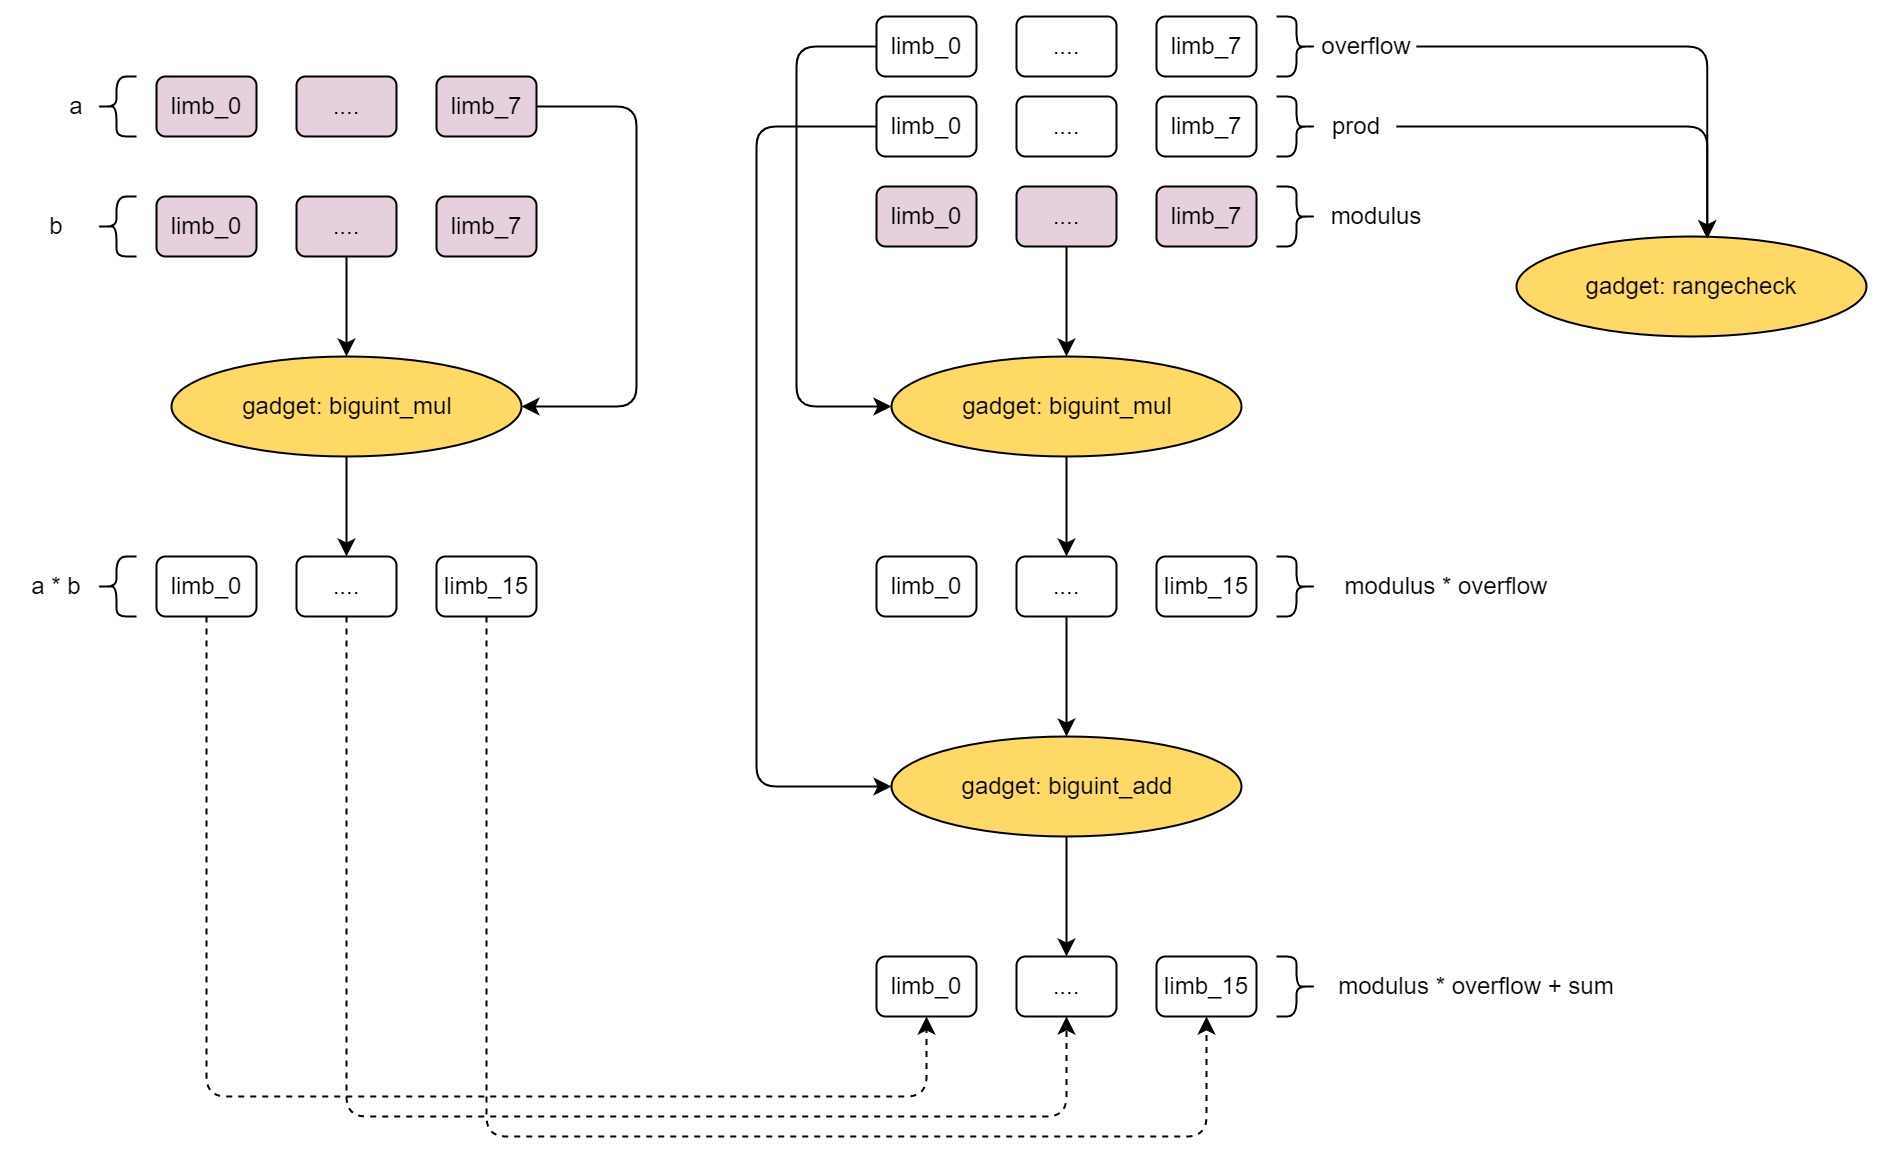
\includegraphics[width=0.8\textwidth]{nonnative-mul-layout.jpg}
            \caption{nonnative-mul layout}
            \label{fig:nonnative-mul-layout}
        \end{figure}
    
    \item constraints-info and costs
        \begin{itemize}
            \item gadget biguint-add num: 1
            \item gadget biguint-mul num: 2
            \item gadget u32rangecheck num: 2
            \item gate type num: 9 = 7(U32AddManyGate{3,5,7,9,11,13,15}) + 1(U32RangeCheckGate) + 1(U32ArithmeticGate)
            \item gate instance num: 37 = 2(u32rangecheck) + 8(biguint-mul: constant-input) + 22(biguint-mul) + 1 + 3(biguint-add)
            \item copy-constraints: 583 = 8 * 2(u32rangecheck) + 3 * 3 + (4 + 6 + 8 + 10 + 12 + 14 + 16) * 4 + (8 * 8) * 3 + 17 * 4 + 18
        \end{itemize}

\end{enumerate}
    \subsubsection{nonnative-inv}

\Par{Target}
Check the modular inverse relation among three nonnative target objects.

\Par{Constraints logic}
\begin{itemize}
    \item Check equation for gadget: \verb|a * inv_a = 1 + modular * div|.
\end{itemize}

\Par{Process layout}
See \figref{fig:nonnative-inv-layout}.
\begin{figure}[!ht]
    \centering
    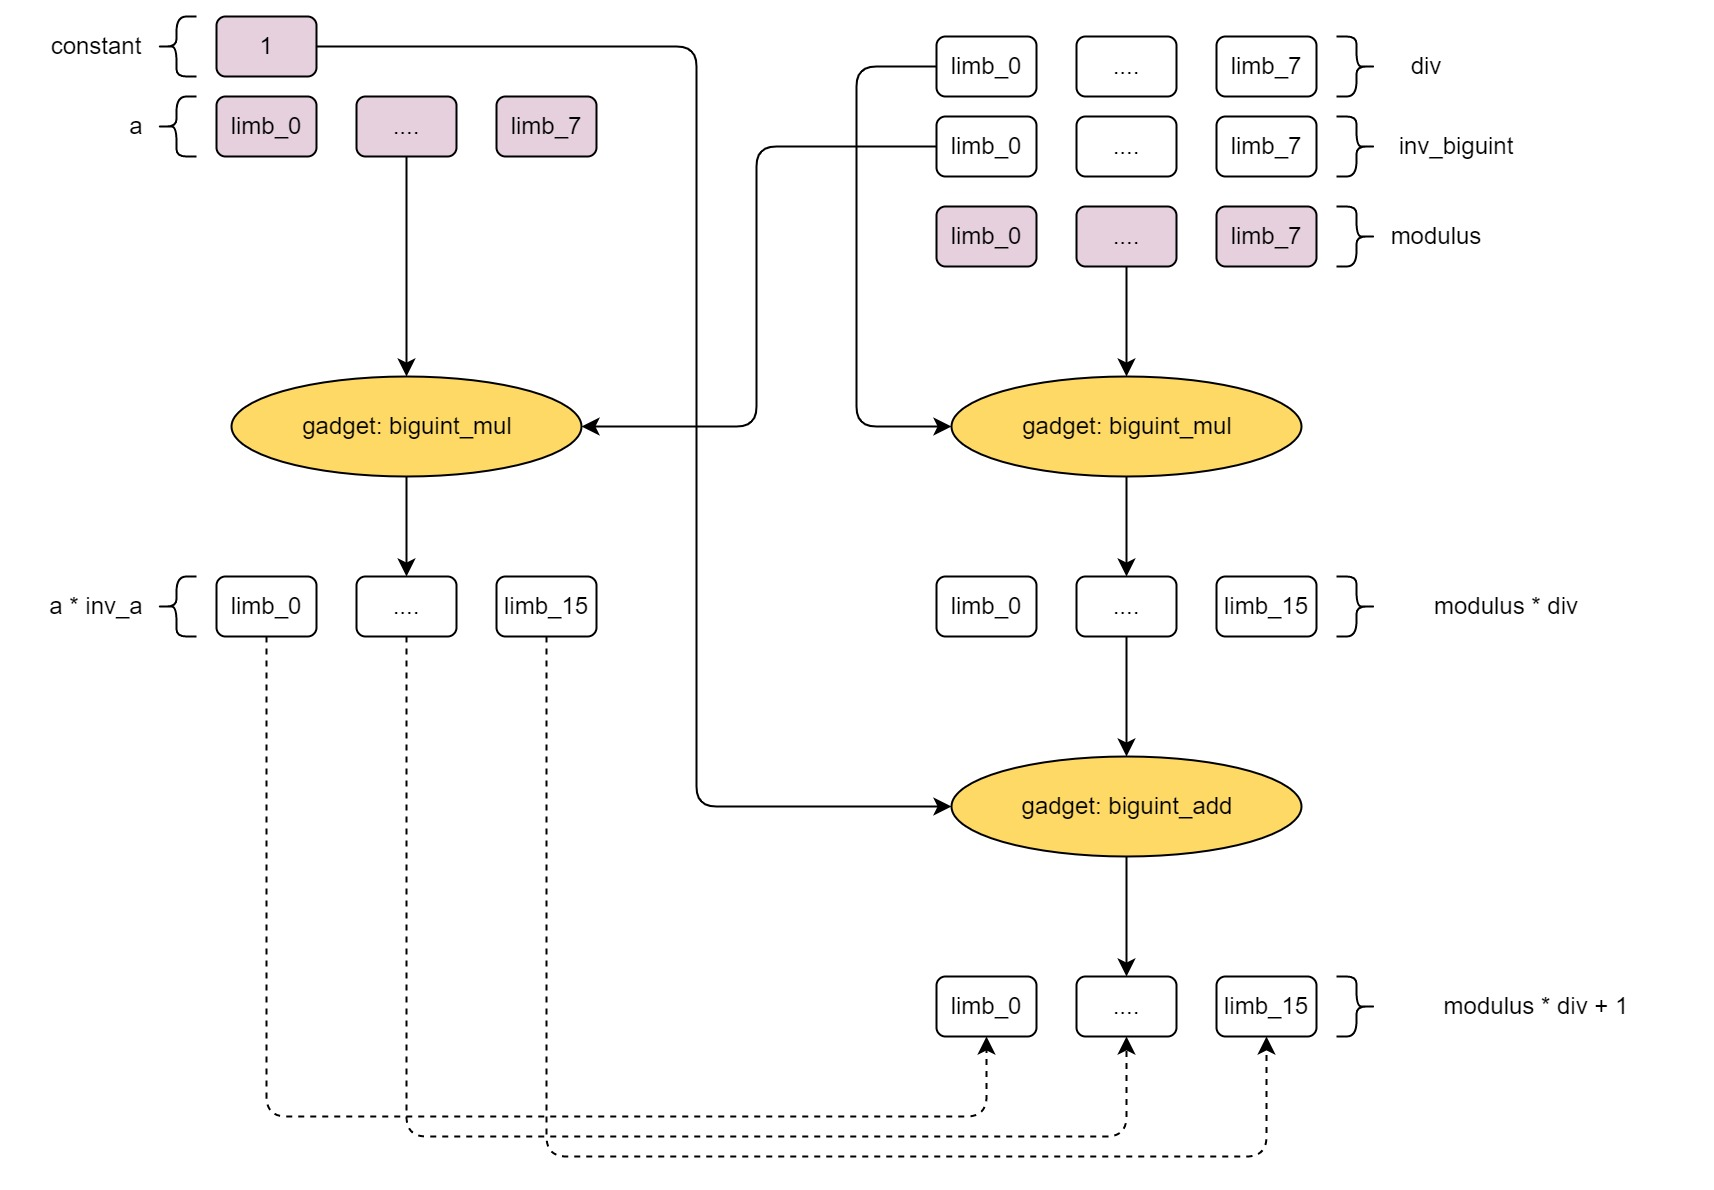
\includegraphics[width=0.8\textwidth]{nonnative-inv-layout.jpg}
    \caption{nonnative-inv layout}
    \label{fig:nonnative-inv-layout}
\end{figure}

\Par{Constraints info and costs}
\begin{itemize}
    \item gadget biguint-add num: 1
    \item gadget biguint-mul num: 2
    \item gate type num: 8 = 7(U32AddManyGate\{3,5,7,9,11,13,15\}) + 1(U32ArithmeticGate)
    \item gate instance num: 56 = (8 * 8 + 2) * 2 / 3 + 5(U32AddManyGate{3}) + 5 + 2(U32AddManyGate{15})
    \item copy-constraints: 762 = (8 * 8 + 2) * 2 * 3 + 21 * 4 + (6 + 8 + 10 + 12 + 14) * 4 + 4 * 16 + 18
\end{itemize}

    \section{curve-add}
\label{curve-add}

Take curve-secp256k1 as example, the same as other texs.

\begin{enumerate}
    \item target
        implement the addition of two different curve points. this is a incomplete addition, you can refer to The halo2 Book \cite{website:halo2-book} to learn more about it.
    \item constraints-logic
        \begin{figure}[!ht]
            \centering
            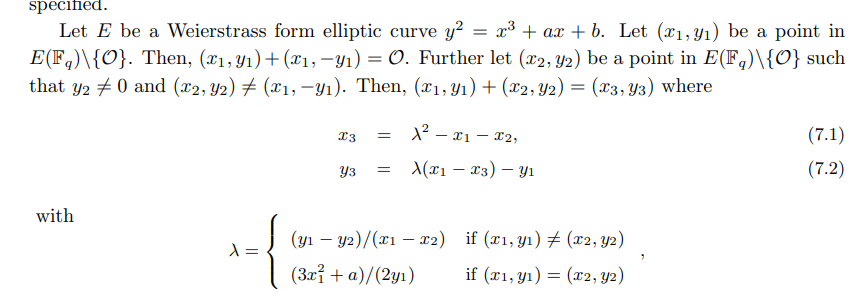
\includegraphics[width=0.8\textwidth]{curve-add.jpg}
            \caption{curve-add}
            \label{fig:curve-add}
        \end{figure}
    \item curve-add process layout
        \begin{figure}[!ht]
            \centering
            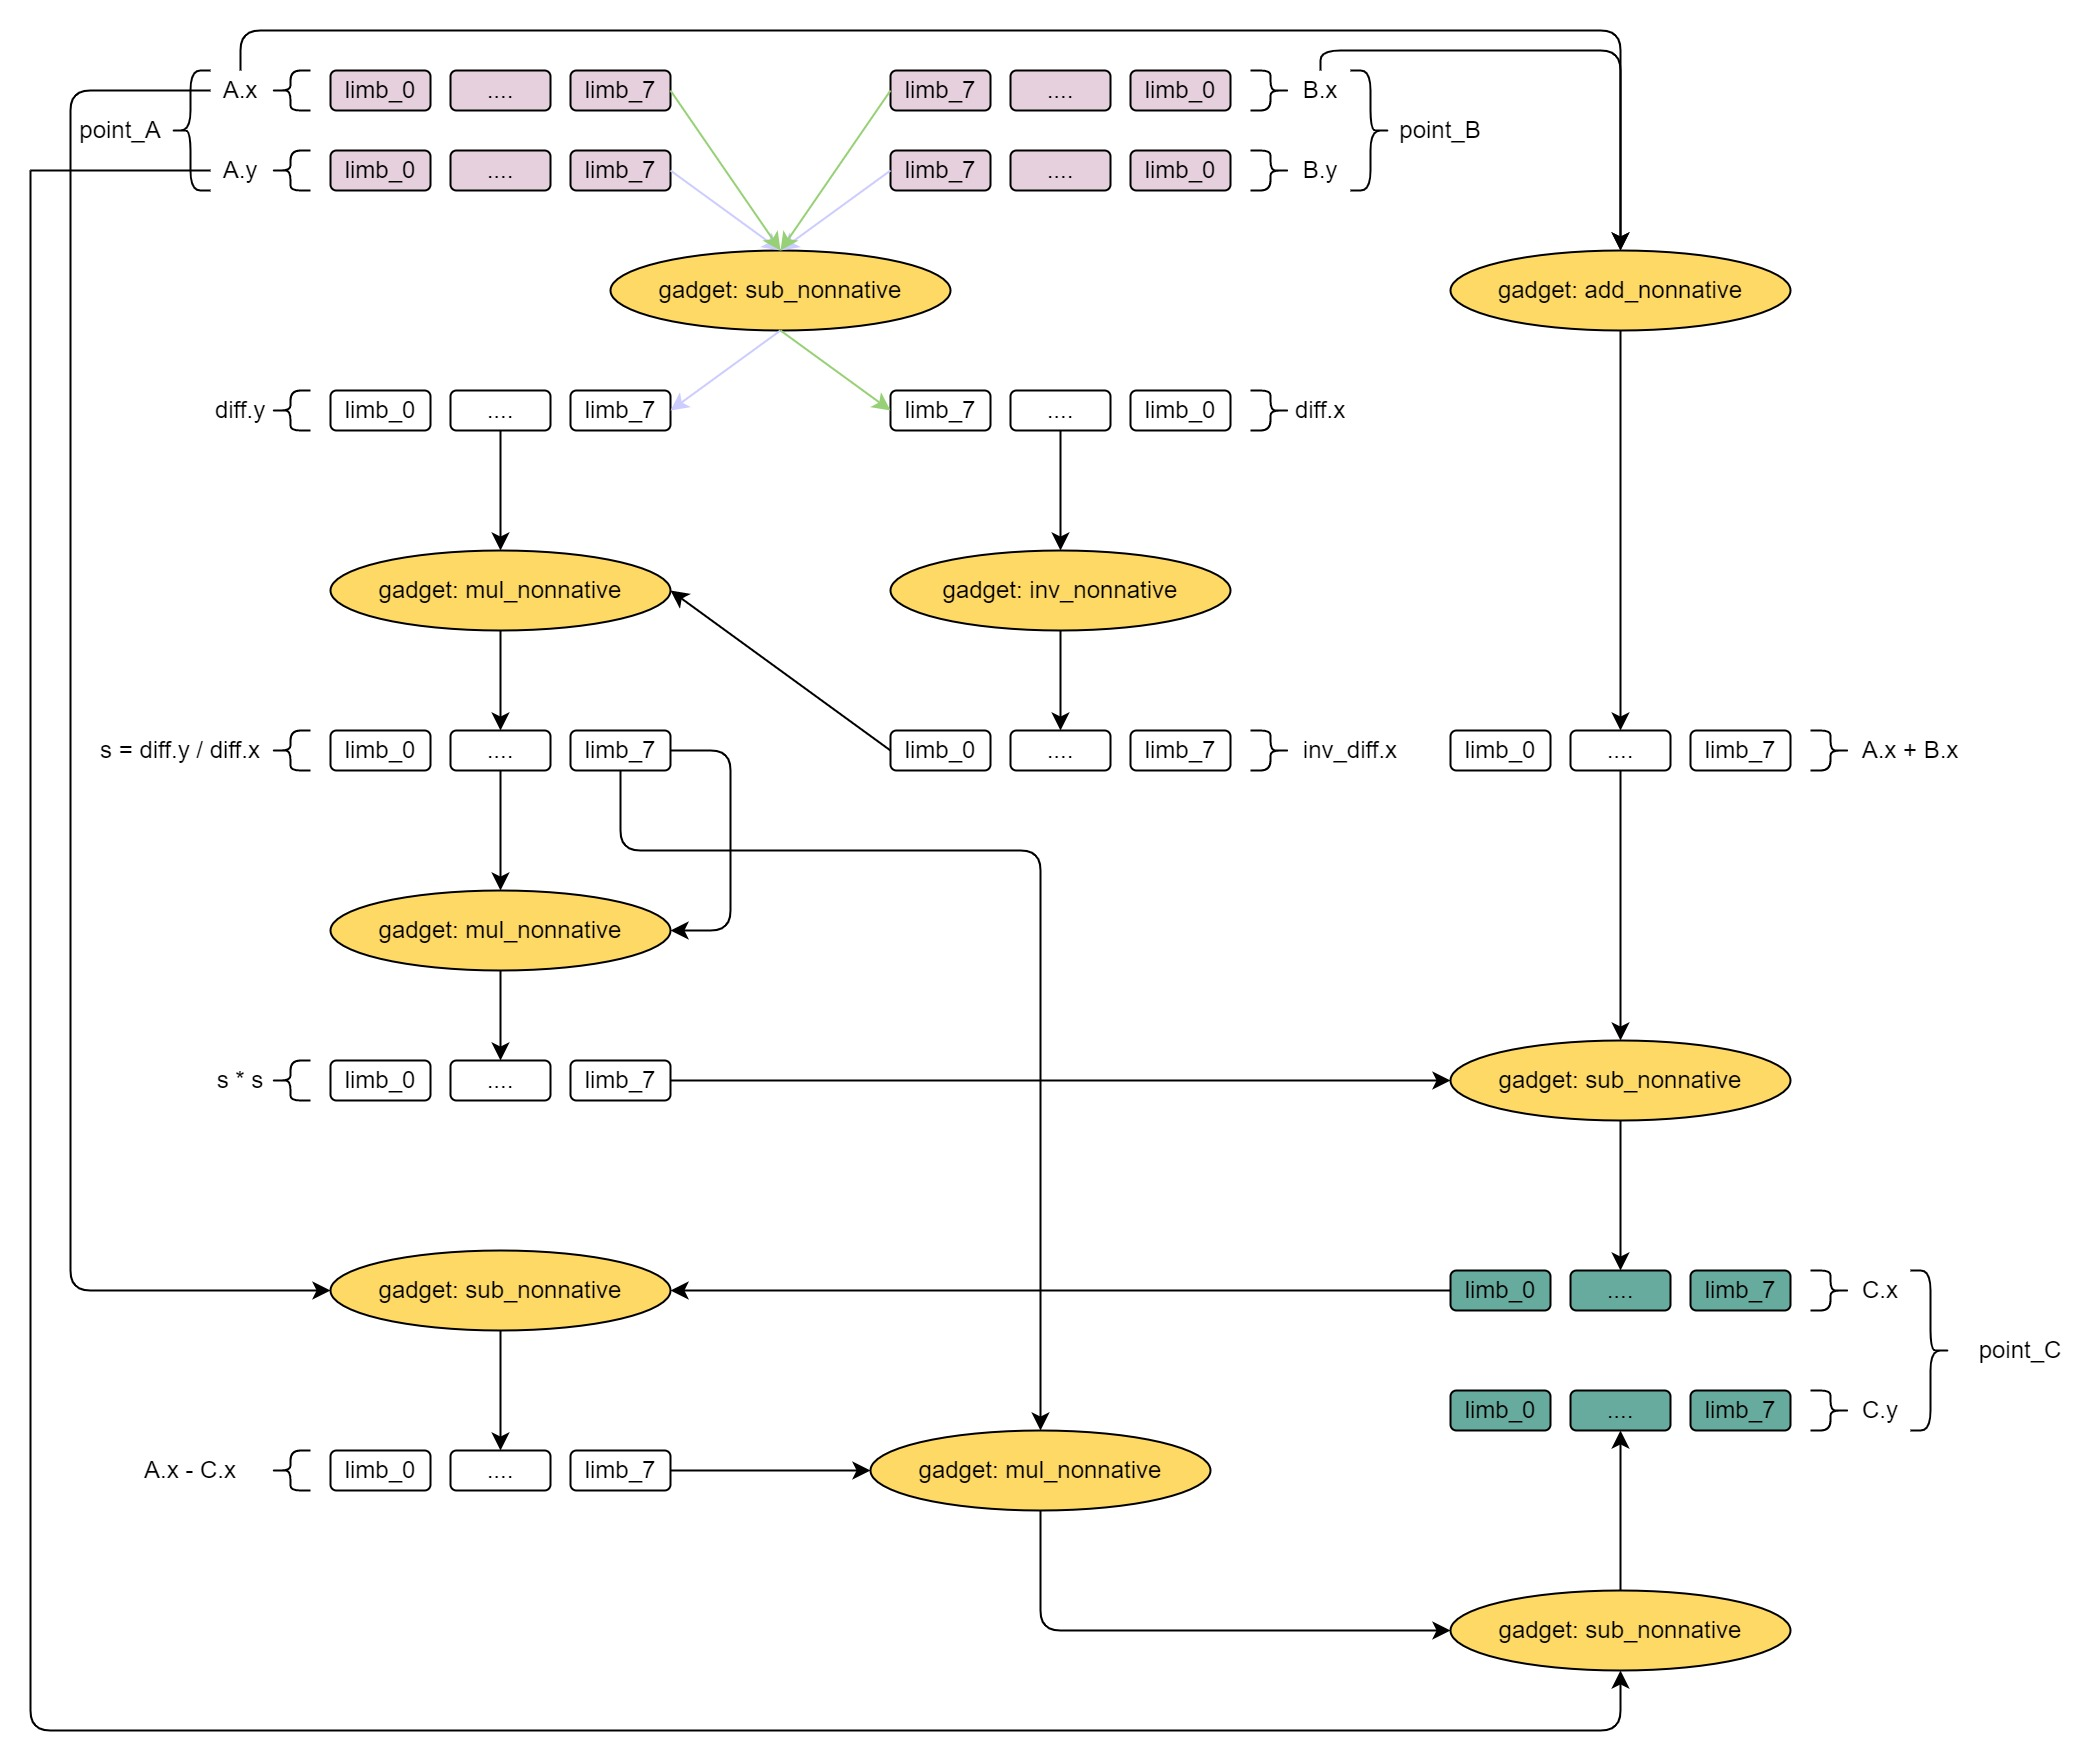
\includegraphics[width=0.8\textwidth]{curve-add-layout.jpg}
            \caption{curve-add layout}
            \label{fig:curve-add-layout}
        \end{figure}
    
    \item constraints-info and costs
        \begin{itemize}
            \item gadget-sub-nonnative num: 5
            \item gadget-add-nonnative num: 1
            \item gadget-mul-nonnative num: 3
            \item gadget-inv-nonnative num: 1
            \item gate type num: 
            \item gate instance num: 
        \end{itemize}

\end{enumerate}
    \subsubsection{curve-double}

\Par{target}
Implement the addition of two same curve points. this is a incomplete addition, you can refer to The halo2 Book \cite{website:halo2-book} to learn more about it.

\Par{Constraints logic}
$(x_1,y_1) = (x_2,y_2)$. See \figref{fig:curve-add}.

\Par{Process layout}
See \figref{fig:curve-double-layout}.
\begin{figure}[!ht]
    \centering
    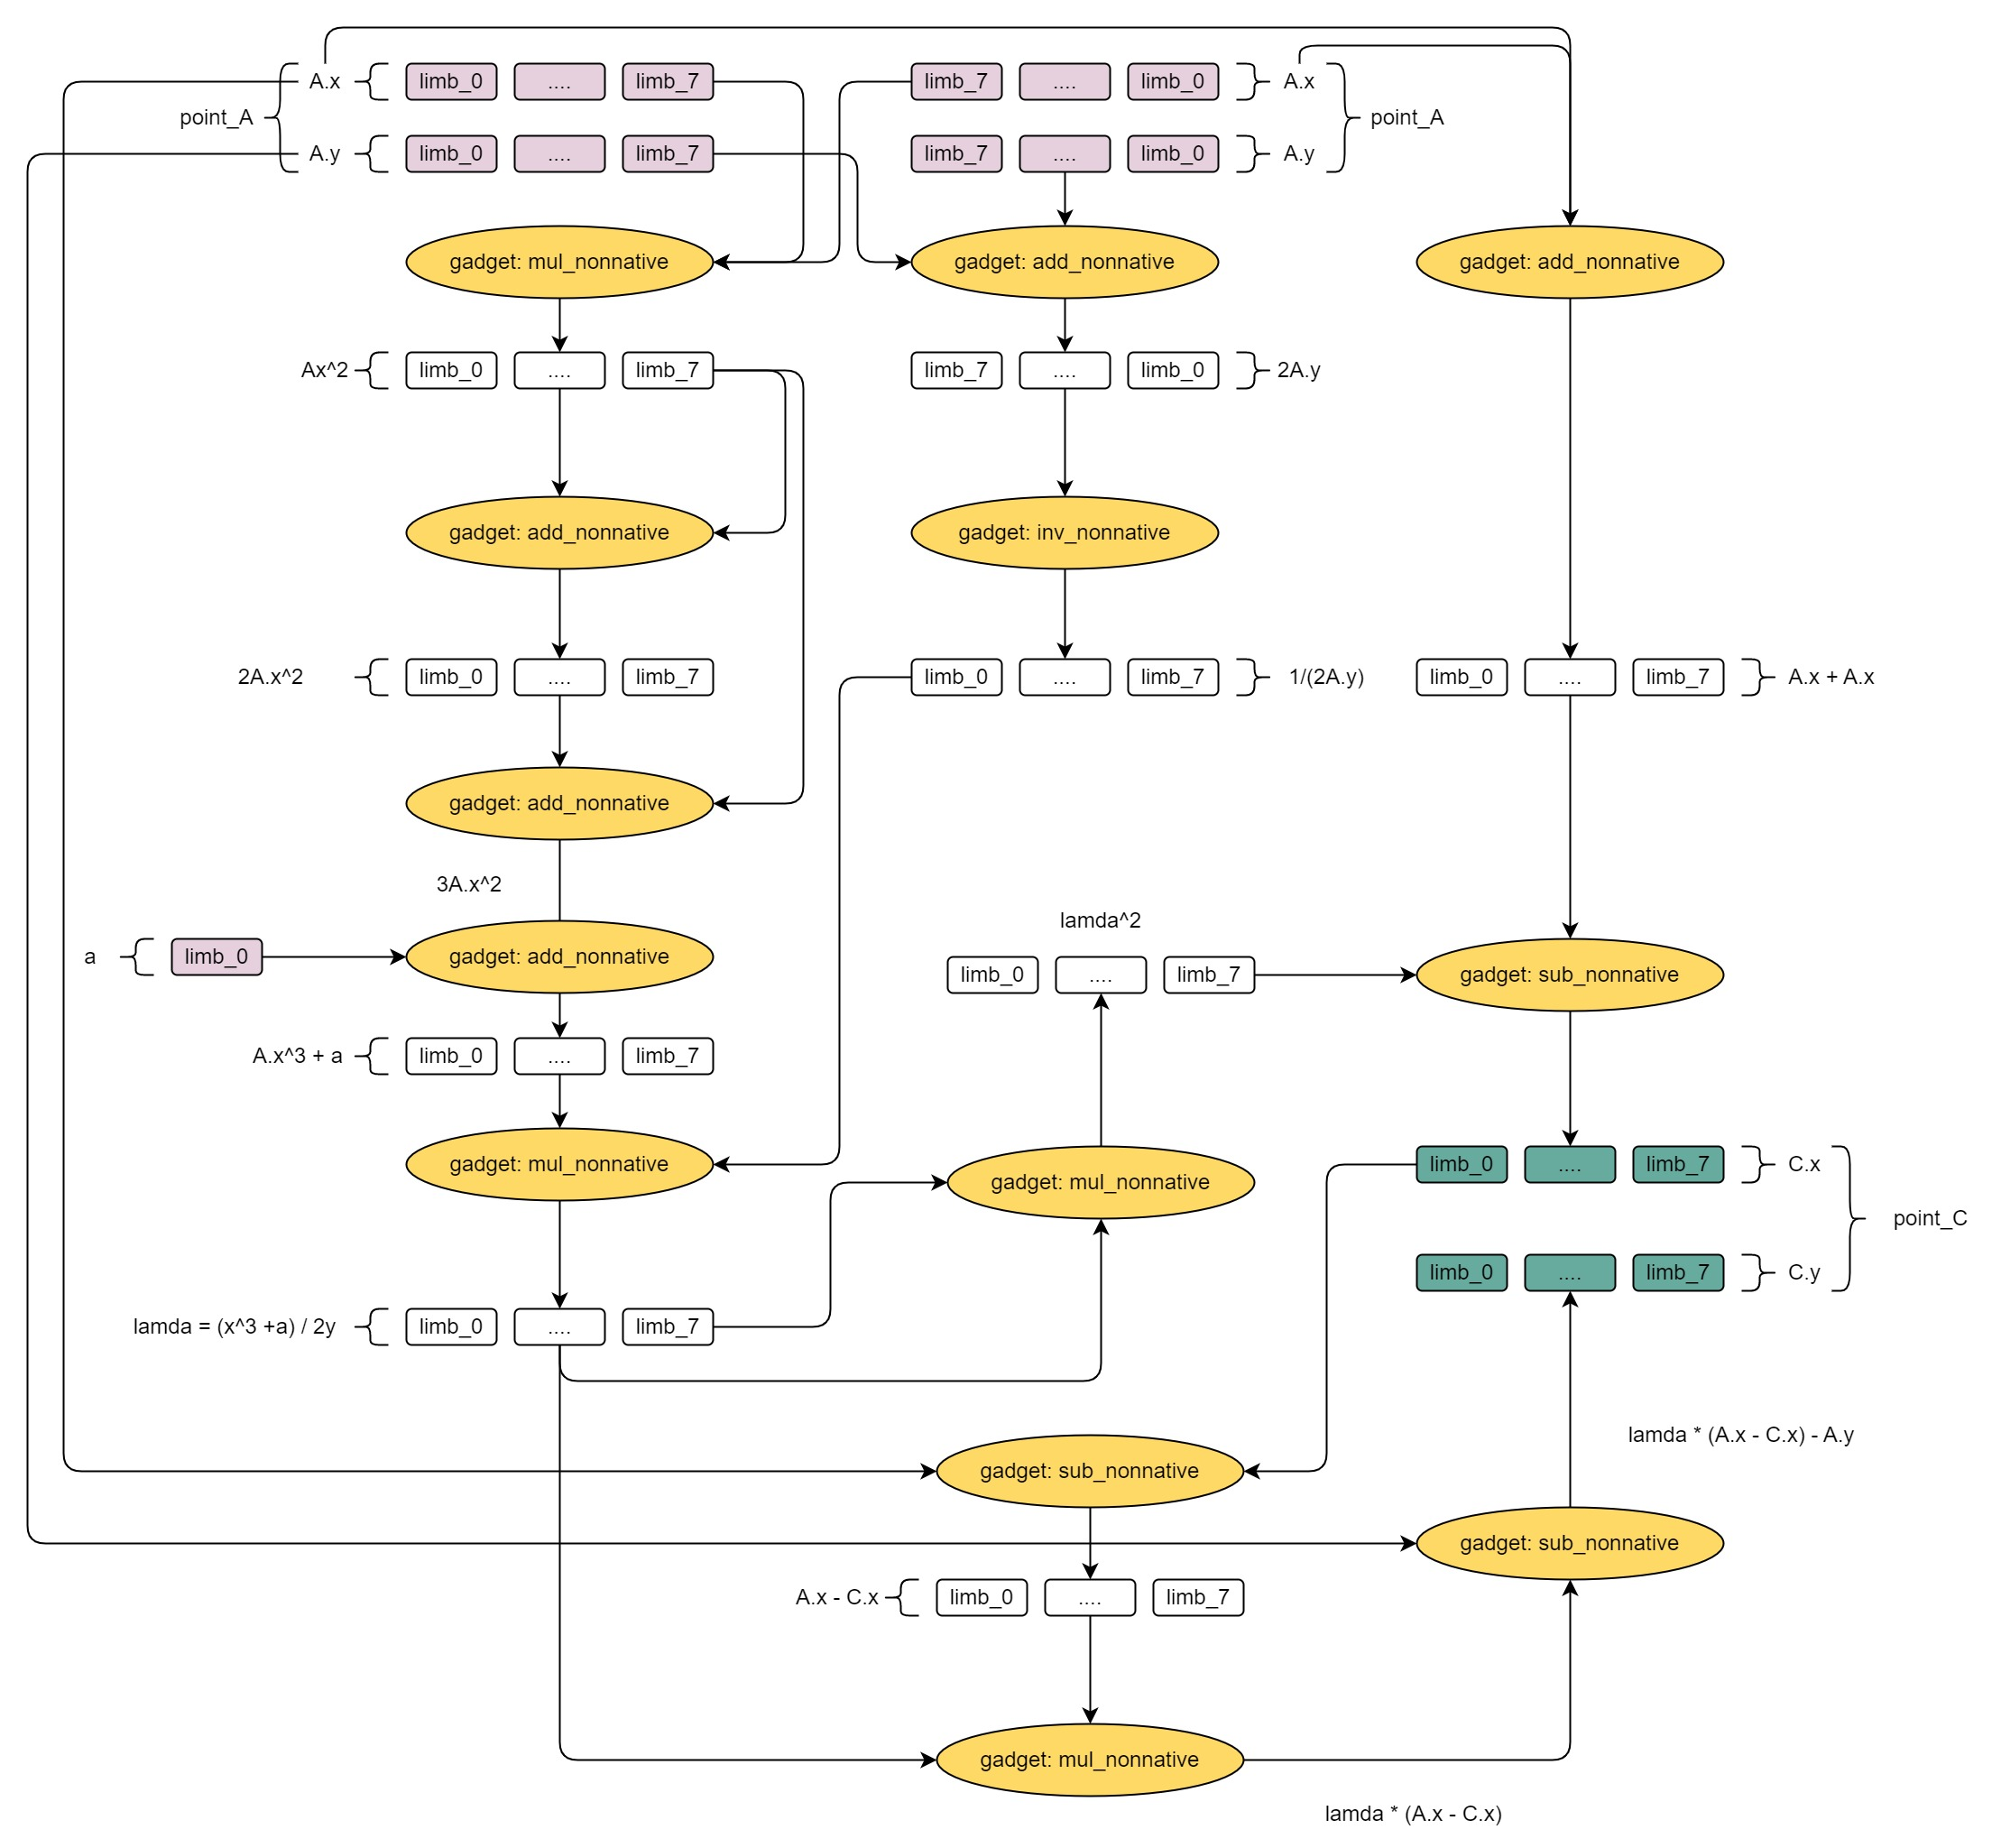
\includegraphics[width=0.8\textwidth]{curve-double-layout.jpg}
    \caption{curve-double layout}
    \label{fig:curve-double-layout}
\end{figure}

\Par{Constraints info and costs}
\begin{itemize}
    \item gadget-sub-nonnative num: 3
    \item gadget-add-nonnative num: 5
    \item gadget-mul-nonnative num: 4
    \item gadget-inv-nonnative num: 1
    \item gate type num: 14
        \begin{itemize}
            \item 8: U32AddManyGate\{2,3,5,7,9,11,13,15\}
            \item 1: ComparisonGate
            \item 1: ArithmeticGate
            \item 1: U32ArithmeticGate
            \item 1: U32SubtractionGate
            \item 2: U32RangeCheckGate\{0,8\}
        \end{itemize}
\end{itemize}

    \subsubsection{curve-assert-valid}
\label{curve-assert-valid}

Take curve-secp256k1 as example, the same as other texs.

\begin{enumerate}
    \item target
        check point is on the curve, y\^2 = x\^3 + ax +b
    \item curve-assert-valid process layout
        \begin{figure}[!ht]
            \centering
            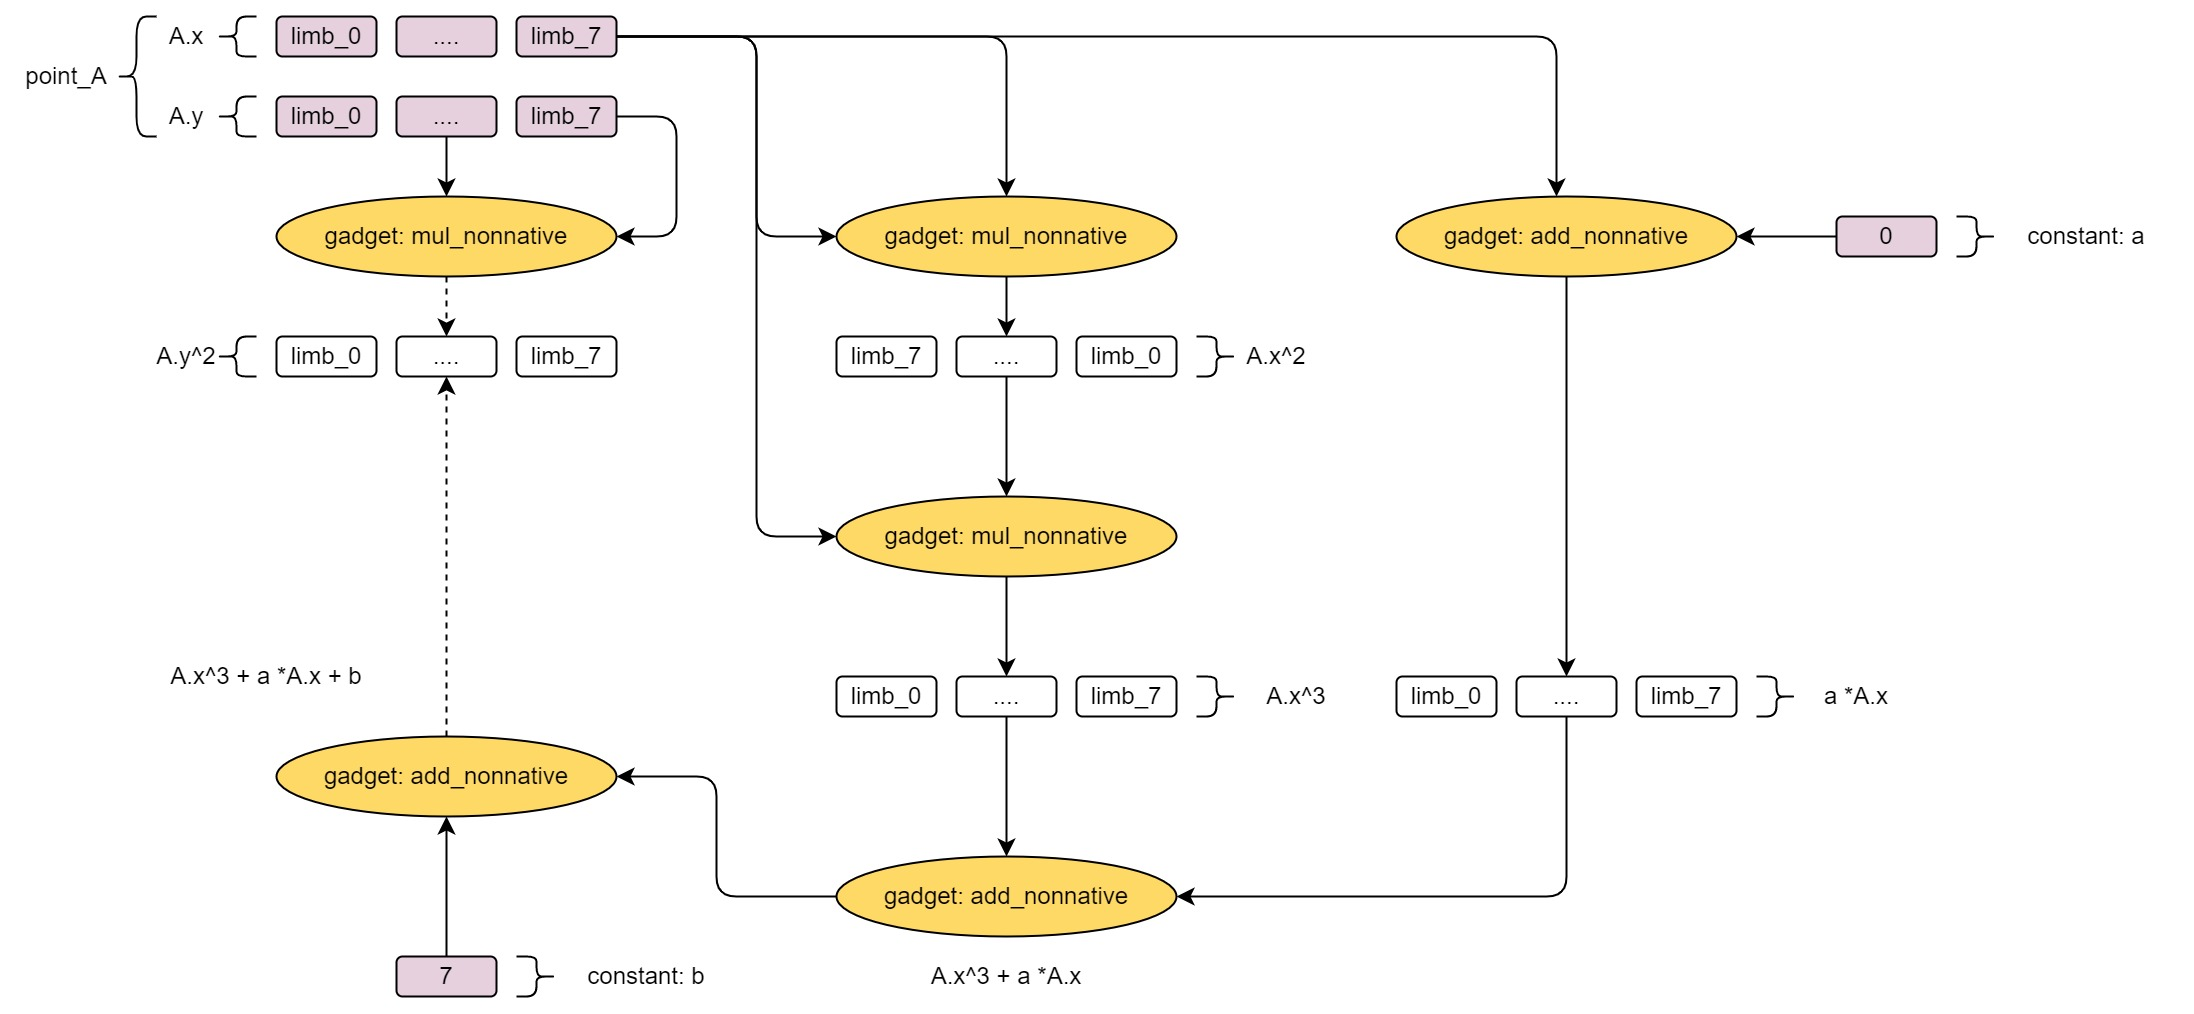
\includegraphics[width=0.8\textwidth]{curve-assert-valid-layout.jpg}
            \caption{curve-assert valid layout}
            \label{fig:curve-assert-valid-layout}
        \end{figure}
    \item constraints-info and costs
        \begin{itemize}
            \item gadget-add-nonnative num: 3
            \item gadget-mul-nonnative num: 3
            \item gate type num: 13
                \begin{itemize}
                    \item 8: U32AddManyGate{2,3,5,7,9,11,13,15}
                    \item 1: ComparisonGate
                    \item 1: ArithmeticGate
                    \item 1: U32ArithmeticGate
                    \item 2: U32RangeCheckGate{0,8}
                \end{itemize}
        \end{itemize}

\end{enumerate}  
    \subsubsection{curve-msm}
\label{curve-msm}

Take curve-secp256k1 as example, the same as other texs.

\begin{enumerate}
    \item target
        implement the multiplication scalar multiplicaiton(msm). 
    \item constraints-logic
        \begin{figure}[!ht]
            \centering
            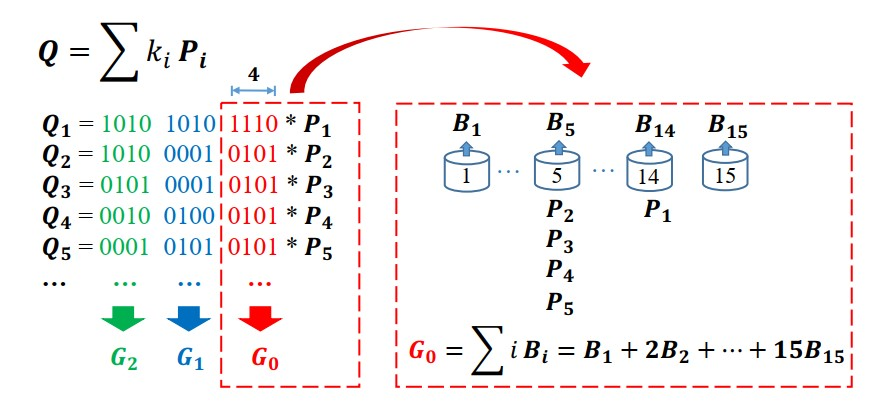
\includegraphics[width=0.8\textwidth]{curve-msm.jpg}
            \caption{curve-msm}
            \label{fig:curve-msm}
        \end{figure}
    
    \item constraints-info and costs
        \begin{itemize}
            \item gate type num: 14
            \item gate instance num: 147553
        \end{itemize}
\end{enumerate}
    \subsubsection{curve-scalar}
\label{curve-scalar}

Take curve-secp256k1 as example, the same as other texs.

\begin{enumerate}
    \item target
        implement the multiplication between scalar and point. 
    \item constraints-logic
        \begin{figure}[!ht]
            \centering
            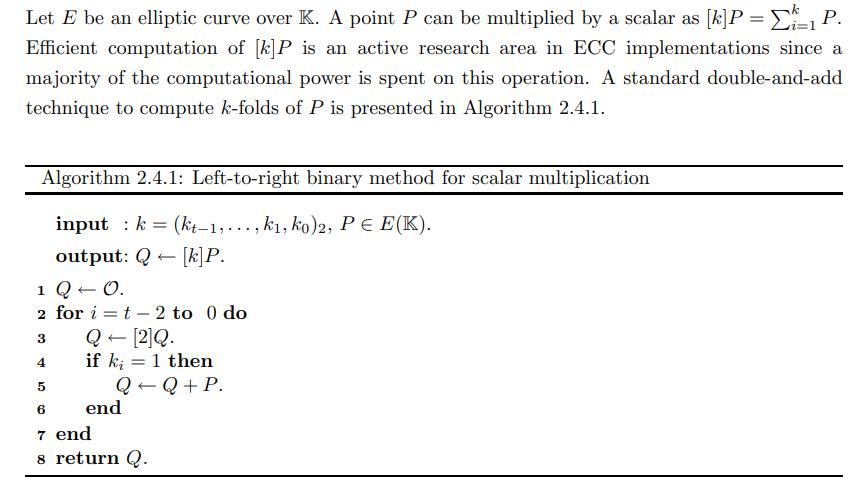
\includegraphics[width=0.8\textwidth]{curve-scalar.jpg}
            \caption{curve-scalar}
            \label{fig:curve-scalar}
        \end{figure}
    
    \item constraints-info and costs
        \begin{itemize}
            \item gate type num: 13 
            \item gate instance num: 180364          
        \end{itemize}
\end{enumerate}
    \subsubsection{ecdsa}
\label{ecdsa}

Take curve-secp256k1 as example, the same as other texs.

\begin{enumerate}
    \item target
        implement ecdsa verify process. 
    \item constraints-logic
        \begin{figure}[!ht]
            \centering
            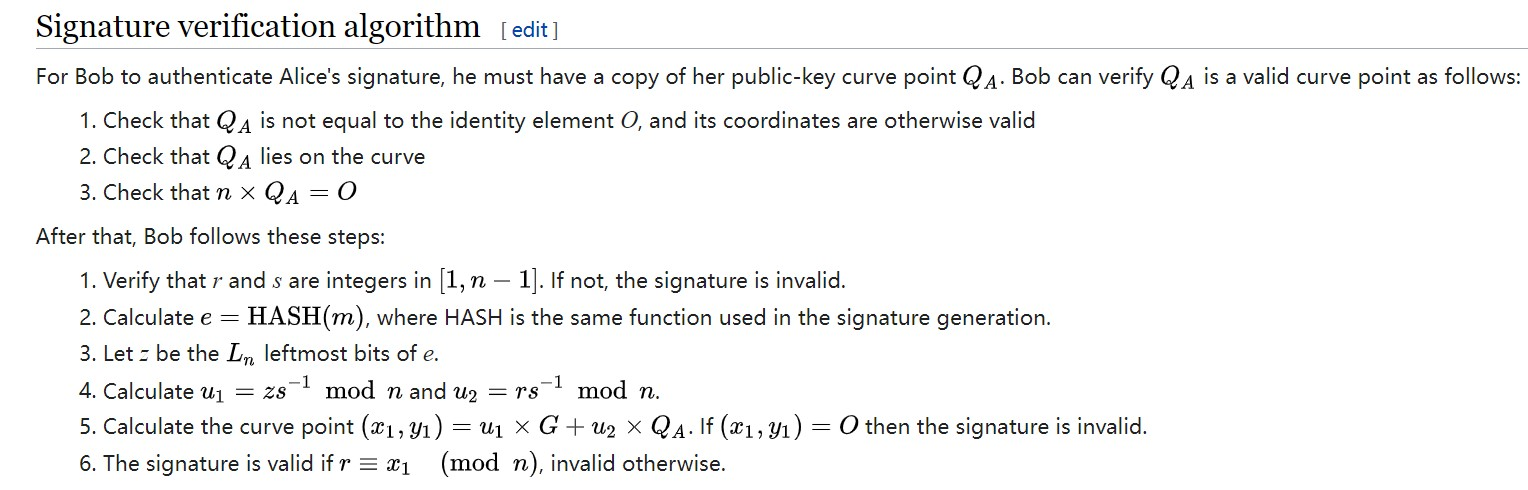
\includegraphics[width=0.8\textwidth]{ecdsa.jpg}
            \caption{ecdsa}
            \label{fig:ecdsa}
        \end{figure}  
    \item constraints-info and costs
        \begin{itemize}
            \item gate type num: 16
            \item gate instance num: 98039
        \end{itemize}
\end{enumerate}
    \subsubsection{circuit-build}

Plonky2 builds a full circuit with both prover and verifier data. The circuit
description in Plonky2 is a data structure that describes the constraint
relationship within the gate and among the gates, which is the same with Plonk.

One of the difference is Plonky2 makes extensive use of custom gates and generates
a trace table with all used custom gates. Each row in the trace table represents
an instance of a type of cutom gates, which can perform a specified operation
designed by developers.

If the config supports enough routed wires, an instance of an arithmetic gate can
support several such operations. When performing an arithmetic operation, Plonky2 
will find an available slot, of the form (row and op) for it and first check if
there is an exist gate instance in the circuit to use, rather than just add a new
one.

For example, U32AddManyGate is a custom gate to perform addition on \verb|num_addends| 
different 32-bit values, plus a small carry. Defaultly, each gate has 80 routed wires
and 135 wires, if \verb|num_addends| is two, then a U32AddManyGate can support five
addition operations.

Suppose we need to perform a new addition of two 32-bit values, and there is an gate
instance of such U32AddManyGate in the circuit, with only three operations used. 
Then we use its fourth op to perform the addition operation.

\begin{figure}[!ht]
    \centering
    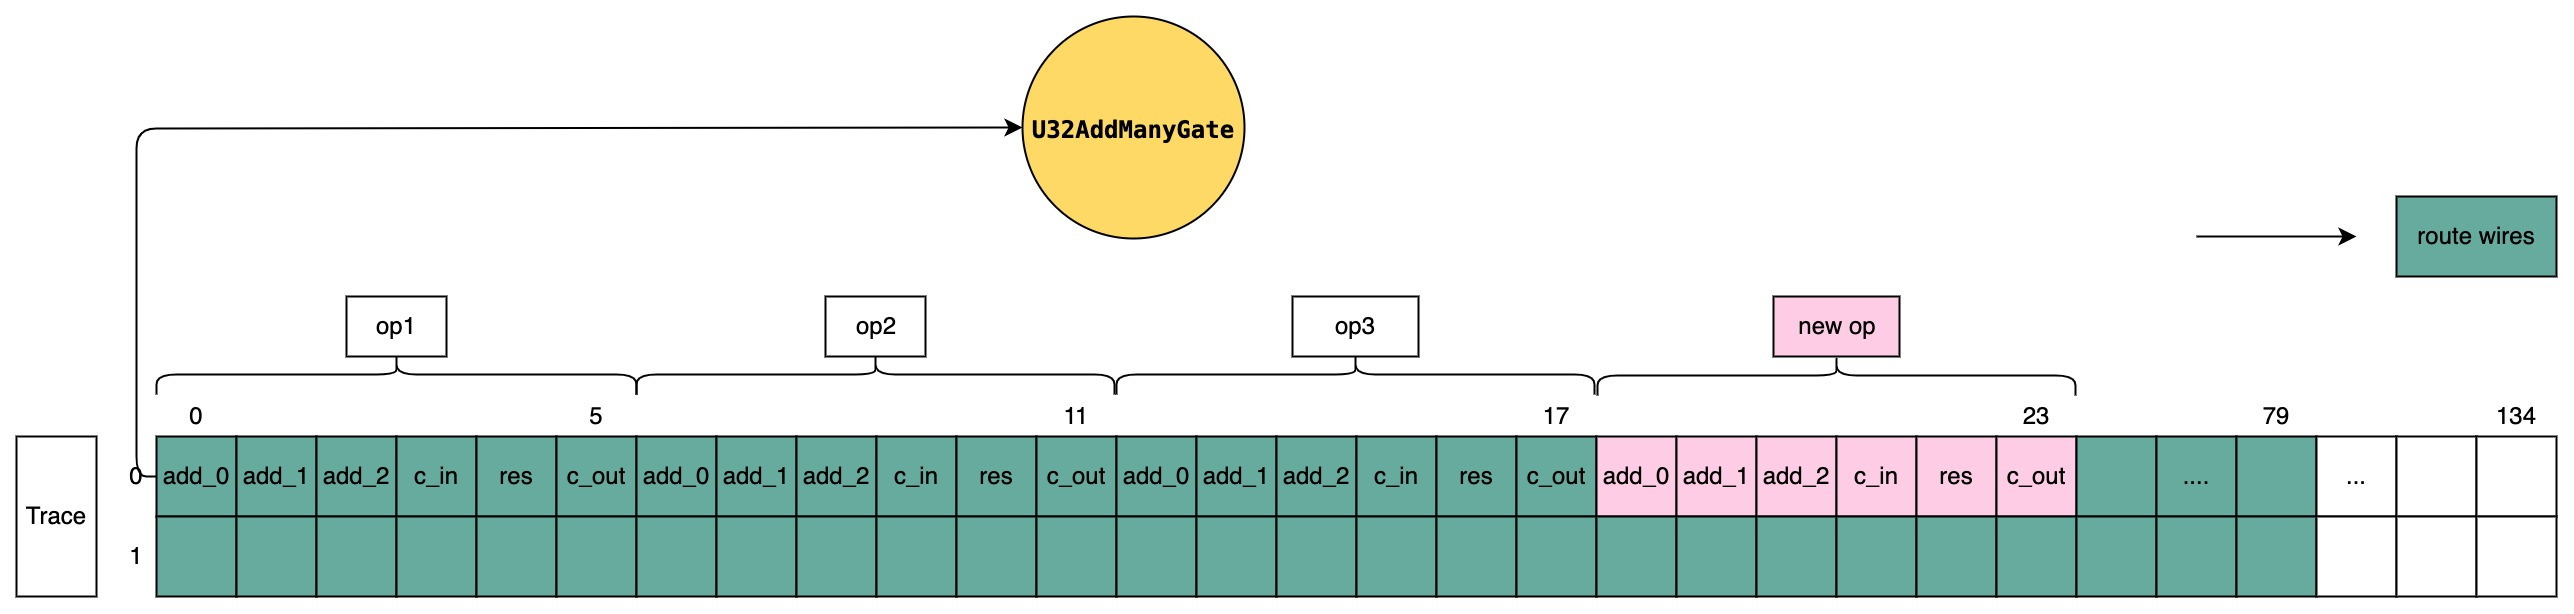
\includegraphics[width=0.8\textwidth]{circuit-build-slot.jpg}
    \label{fig:circuit-build-slot}
\end{figure}

If no instance of such U32AddManyGate in the circuit or all instances of U32AddManyGate are
full, then we need to add a new instance of U32AddManyGate with two addends to the circuit,
which also adds a new row to the trace table.

Once all instances of custom gates are added to the circuit, the constraints of all gates
are also determined in the trace table. To simplify generate filter polynomials in prove
phase, see \href{https://hackmd.io/@sin7y/H10EO2Z5q#Combined-selector}{combined selector},
Plonky2 calculates all selector polynomials and related information in advance.

Before computing the selector polynomials, Plonky2 sorts all gates by their degrees and ID
to make the ordering deterministic. Then partition the gates into several groups. For each
group G, the number of gates in it plus each gate's degree are less than or equal to the 
max degree of configuration:
\[ |G| + \max_{g \in G}\{\text{g.degree()}\} \le \text{max\_degree}. \]

The reason behind it is in prove phase, Plonky2 will calculate the filter polynomials and
multiply them with custom gates' constraint polynomials, the result is a polynomial whose 
degree is equal to $|G| + \text{gate.degree()}$. These groups are constructed greedily from the 
list of gates sorted by degree and ID.

After finishing partitioning groups, Plonky2 builds a selector polynomial for each group. 
For instance, a circuit uses four ordered gates: add, sub, div and mul. The four gates are
partitioned into two groups: g1 \{ add, sub \} and g2 \{ div, mul \}. Each gate has and only has
one instance, that is there are four rows in its trace:

\begin{center}
    \begin{tabular}{ |c|c|c|c|c|c| }
        \hline
        row  & w0 & w1 & w2 & w3 & gate \\
        \hline
        0  & a0 & b0 & c0 & d0 & div \\
        \hline
        1  & a1 & b1 & c1 & d1 & mul \\
        \hline
        2  & a2 & b2 & c2 & d2 & add \\
        \hline
        3  & a3 & b3 & c3 & d3 & sub \\
        \hline
    \end{tabular}
\end{center}

To understand the process of building polynomials from groups, we first add a new column to the
trace table to simulate the polynomial of group g1. For each row in the trace table, the value of the cell is
the gate index if the gate is in g1, otherwise unused, which defined by Plonky2 is u32::MAX:

\begin{center}
    \begin{tabular}{ |c|c|c|c|c|c|c| }
        \hline
        row & g1 & w0 & w1 & w2 & w3 & gate \\
        \hline
        0 & unused & a0 & b0 & c0 & d0 & div \\
        \hline
        1 & unused & a1 & b1 & c1 & d1 & mul \\
        \hline
        2 & 0 & a2 & b2 & c2 & d2 & add \\
        \hline
        3 & 1 & a3 & b3 & c3 & d3 & sub \\
        \hline
    \end{tabular}
\end{center}

Then we add another column of g2 to the trace and fill the values with same rule:

\begin{center}
    \begin{tabular}{ |c|c|c|c|c|c|c|c| }
        \hline
        row & g1 & g2 & w0 & w1 & w2 & w3 & gate \\
        \hline
        0 & unused & 2 & a0 & b0 & c0 & d0 & div \\
        \hline
        1 & unused & 3 & a1 & b1 & c1 & d1 & mul \\
        \hline
        2 & 0 & unused & a2 & b2 & c2 & d2 & add \\
        \hline
        3 & 1 & unused & a3 & b3 & c3 & d3 & sub \\
        \hline
    \end{tabular}
\end{center}

Now we have two new columns with four values, we can construct two selector polynomials from 
them easily.

Apart from selector polynomials, Plonky2 also generates several constant polynomials and sigma
polynomials, then commits these polynomials all together and generates a merkle tree, which is 
used in FRI. The last thing calculated in circuit build phase is generators, which store all 
information of performing operations and generating constants in the circuit. They are used to
generate full witness in prove phase.

At the end of circuit build, Plonky2 returns circuit data incluing three data structures:

Common data:

\begin{lstlisting}[language=rust]
    let common = CommonCircuitData {
        config: self.config, // circuit config
        fri_params, // fri config
        gates, // types of gates used in circuit
        selectors_info, // information of groups and selector polynomials
        quotient_degree_factor, // the degree of the PLONK quotient polynomial
        num_gate_constraints, // the largest number of constraints imposed by any gate
        num_constants, // the number of constant wires
        num_public_inputs, // the number of public inputs
        k_is, // shifts used in lde
        num_partial_products, // number of partial products in generating Z(x)
    }
\end{lstlisting}

Prover data:

\begin{lstlisting}[language=rust]
    let prover_only = ProverOnlyCircuitData {
        generators: self.generators, // store information of all operations and used to generate full witness
        generator_indices_by_watches, // used to perform operations dependent on other operations
        constants_sigmas_commitment, // commitment of selector polynomials, constant polynomials and sigma polynomials
        sigmas: transpose_poly_values(sigma_vecs), // the transpose of the list of sigma polynomials
        subgroup, // subgroup of order `degree`
        public_inputs: self.public_inputs, // targets to be made public
        representative_map: forest.parents, // store information of copy constrains
        fft_root_table: Some(fft_root_table), // intermediate values used in fft
        circuit_digest, // a digest of the circuit, which can be used to seed Fiat-Shamir
    }
\end{lstlisting}

Verifier data:

\begin{lstlisting}[language=rust]
    let verifier_only = VerifierOnlyCircuitData {
        constants_sigmas_cap, // a commitment to each constant polynomial and each permutation polynomial
        circuit_digest, // a digest of the circuit, which can be used to seed Fiat-Shamir
    }
\end{lstlisting}

    %\printbibliography[heading=bibintoc, title=\ebibname]%
\end{document}
